\part{Global methods for sampling rare diffusive events}

\chapter{Ritz methods for Freidlin-Wentzel-Graham actions} \label{ch:Ritz methods for Freidlin-Wentzel-Graham actions}

\section{Introduction}

The theory of Freidlin, Wentzell and Graham \citep{wentzellSmallRandomPerturbations1970, graham1973statistical,graham1987macroscopic}
gives asymptotic probability estimates of rare events in dynamical
systems perturbed by small noise \citep{bolhuisTransitionPathSampling2002a, allen2005sampling, allen2009forward, ebenerInstantonBasedImportance2019b}.
Specifically, Freidlin-Wentzell-Graham (FWG) theory yields estimates of the stationary
distributions and mean first-passage times. Both these quantities
are determined, in turn, by the asymptotic estimate of the probability
of a stochastic trajectory to not deviate from a smooth path by more
than a given amount in a given interval of time. The key result of
FWG is that the limiting form of this probability,
for small noise and small deviations, is given by a non-negative functional
of the smooth path. This functional is known as the \textit{Freidlin-Wentzell action} and its minimum, for fixed initial and terminal states, determines
both the stationary distributions and first-passage times. The smooth
path minimising the action is often called the Freidlin-Wentzell instanton.
The theory is applicable to dynamical systems of both gradient and
non-gradient character and can so be used to study a wide variety
of equilibrium and non-equilibrium systems modelled by Itô diffusions
\citep{paninskiMostLikelyVoltage2006a, huangMolecularMathematicalBasis2012a, bouchet2016generalisation, maier1996scaling, wolynesNavigatingFoldingRoutes1995a, noltingBallsCupsQuasipotentials2016a, mangelBarrierTransitionsDriven1994a, gardnerConstructionGeneticToggle2000a, demarcoPhaseTransitionModel2001a, nelson1987stochastic}.

Determining the minimum of the Freidlin-Wentzell action is a problem
in the calculus of variations. The Euler-Lagrange equations provide
the necessary conditions for extrema of variational problems and,
unsurprisingly, have been the basis of the large literature devoted
to the numerical computation of Freidlin-Wentzell instantons \citep{weinanStringMethodStudy2002, paninskiMostLikelyVoltage2006a, vanden-eijndenGeometricMinimumAction2008b, grafkeLongTermEffects2017}.
There exists, however, an alternative ``direct'' route for the solution
of variational problems in which the functional is reduced, through
finite-dimensional parametrisations of paths, to a multivariate function
and then extremised by appropriate multivariate
optimisation methods \citep{gelfandCalculusVariations2012a, kantorovich1958approximate}.
To the best of our knowledge, the first use of the direct method for
the Freidlin-Wentzell action, discretised by finite-differences, appears
in the work of Weinan, Ren and Vanden-Eijnden \citep{eMinimumActionMethod2004a}. 

Here we combine the direct method with a Ritz discretisation \citep{ritz1909uber, gelfandCalculusVariations2012a, kantorovich1958approximate}
to minimize the Freidlin-Wentzell action. We analyse paths in a spectral
basis of Chebyshev polynomials and use spectral quadrature to express
the action as a multivariate function of the basis coefficients. Nonlinear
optimisation is used to obtain coefficients that give the least action
from which the instanton is synthesised in the spectral basis.\textcolor{black}{{}
For minimisation over paths regardless of their duration, this procedure
is especially effective when applied to a reparametrisation-invariant
on-shell form of the action that follows from the time-translational
invariance of the Lagrangian. This generalises the scalar work functional
of Olender and Elber (for gradient dynamics) and the geometric action
of Heyman and Vanden-Eijnden} \citep{vanden-eijndenGeometricMinimumAction2008b} (for non-gradient
dynamics). Our method is efficient enough to robustly sample the logarithm
of the asymptotic estimate of the stationary distribution, \emph{i.e.
}the quasipotential, avoiding the alternative, but numerically delicate,
route of solving the Hamilton-Jacobi equation \citep{cameron2012finding, yang2019computing, dahiyaOrderedLineIntegral2018a}.
Our method is simple to use, converges rapidly, and is applicable
to both equilibrium and non-equilibrium problems. Its implementation
is freely available on GitHub as the open-source Python library PyRitz. 

The remainder of this chapter is organized as follows. In the next section,
we recall key results of Freidlin-Wentzell theory from dual perspectives
of Itô stochastic differential equations and the corresponding Fokker-Planck
equations.\textcolor{black}{{} Sec.~\ref{sec:Minima-of-the-action}
we present the derivation of the on-shell form of the Freidlin-Wentzell
action in a manner reminiscent of the Routh reduction procedure in
classical mechanics and explain its relation to the scalar work and
the geometric action. }In Sec.~\ref{sec:direct-method} we describe
the direct method for the minimisation of functionals, the Chebyshev
spectral basis in which we construct smooth paths, the spectral quadrature
rule we use to evaluate the action, and the multivariate non-linear
optimisation methods we employ to find the minimum. In Sec.~\ref{sec:pyritz-applications}
we apply the direct method to three well-known diffusion processes
and demonstrate convergence in each case. 

A particular achievement of our approach is its relatively facile
ability to calculate quasipotentials. This can be done with a sufficiently
high density of sample points to construct effectively continuous
maps of the quasipotential, which we do here for the same set of benchmark
problems. We conclude with a discussion on extending the method to
degenerate diffusion processes, systems with inertia and to the stochastic
dynamics of fields. 

\section{Large deviation theory} \label{sec:fwtheory}

We consider the autonomous dynamics of a $d$-dimensional coordinate
$X=(X^{1},\ldots,X^{d})$ in $\mathbb{R}^{d}$ perturbed by configuration-dependent
noise of intensity $\sqrt{\varepsilon}$ described by the Itô diffusion
equation \citep{oksendalStochasticDifferentialEquations2003, shreveStochasticCalculusFinance2005}
\begin{equation}
dX^{\mu}=a^{\mu}(X)dt+\sqrt{\varepsilon}\sigma_{\nu}^{\mu}(X)dW^{\nu}\label{general ito diffusion}
\end{equation}
governing the stochastic trajectory $X(t)$, where $a^{\mu}(X)$ is
the drift vector, $\sqrt{\varepsilon}\sigma_{\nu}^{\mu}(X)$ is the
volatility, $W^{\nu}(t)$ is a $d$-dimensional Wiener process and
repeated indices are summed over.  Eq.~\ref{general ito diffusion} is also often referred to as an \textit{overdamped Langevin equation}.

The transition probability density
of the process, $P_{1|1}(x,t|x_{0})=P(X(t)=x|X(0)=x_{0})$, obeys
the Fokker-Planck equation $\partial_{t}P(x|x_{0})=\mathcal{L}P(x|x_{0})$
where the Fokker-Planck operator is

\emph{
\begin{equation}
\begin{aligned}\mathcal{L}(x) & =-\frac{\partial}{\partial x^{\mu}}a^{\mu}(x)+\frac{\varepsilon}{2}\frac{\partial^{2}}{\partial x^{\mu}\partial x^{\nu}}b^{\mu\nu}(x)\end{aligned}
\label{eq:fokker-planck}
\end{equation}
}and \textbf{$b^{\mu\nu}(x)=\sigma_{\lambda}^{\mu}(x)\sigma_{\sigma}^{\nu}(x)\delta^{\lambda\sigma}$}
is the diffusion tensor. We assume it to be non-degenerate, positive-definite
and invertible. The inverse, $b_{\mu\nu}(x)$, induces a Riemannian
structure in $\mathbb{R}^{d}$ with a norm $|x|_{b}=\sqrt{b_{\mu\nu}x^{\mu}x^{\nu}}$
that is distinct from the Euclidean norm $|x|=\sqrt{(x^{1})^{2}+\ldots(x^{d})^{2}}.$
We use the subscript $b$ to indicate this second ``diffusion''
norm. The stationary density satisfies the time-independent Fokker-Planck
equation $\mathcal{L}P_{1}(x)=0$ and, when it exists, is reached
asymptotically in time for arbitrary initial distributions, $\lim_{t\rightarrow\infty}P_{1|1}(x,t|x_{0})=P_{1}(x)$.
The stationary distribution is unique for ergodic
systems \citep{pavliotisStochasticProcessesApplications2014a}. 

Associated with the Itô process is the Freidlin-Wentzell ``action''
functional \citep{wentzellSmallRandomPerturbations1970, graham1973statistical, graham1987macroscopic}
\begin{equation}
S[x(t)]=\frac{1}{2}\int_{0}^{T}|\dot{x}-a(x)|_{b}^{2}dt\label{eq:Freidlin-Wentzell action}
\end{equation}
which gives an asymptotic estimate for the logarithm of the probability
of trajectories $X(t)$ to remain in the tubular neighbourhood of
a smooth path $x(t)$ over the duration $0\le t\leq T$. We write
this as
\begin{equation}
P_{\text{tube}}[x(t)]\asymp\exp\left(-\frac{1}{\varepsilon}S[x(t)]\right)\label{eq:FW-LDP}
\end{equation}
which, in terms of limits, means

\[
S[x(t)]=\lim_{\delta\to0}\lim_{\varepsilon\to0}-\varepsilon\ln P\left[\sup_{0\leq t\leq T}|X(t)-x(t)|_{b}<\delta\right].
\]
The limits must be taken in the order above as they do not commute.
Eq.~\ref{eq:FW-LDP} is a large deviation principle for trajectories
of Itô processes, due to Wentzell and Freidlin and Graham \citep{touchetteLargeDeviationApproach2009}.

For reasons described below, it is of interest to obtain the mode
of the tube probability over the set of continuous paths
\[
\gamma_{T}=\{x(t)\,|\,x(0)=x_{1},x(T)=x_{2},0\leq t\leq T)\}
\]
which have fixed termini $x_{1}$ and $x_{2}$ and are of duration
$T.$ This is equivalent to the variational problem of minimising
the Freidlin-Wentzell action. The minimum value of the action,

\begin{equation}
V_{T}(x_{2}|x_{1})=\min_{\gamma_{T}}S[x(t)],
\end{equation}
is called the quasipotential. The path attaining the minimum,

\begin{equation}
x_{T}^{*}(t)=\arg\,\min_{\gamma_{T}}\,S[x(t)],
\end{equation}
is called the instanton. We emphasise that this path describes the
smooth centerline of the tube of maximum probability and not a non-differentiable
trajectory of the diffusion process. It is the most probable dynamical
path connecting two points in configuration space. 

The instanton and the quasipotential are central objects in Freidlin-Wentzell-Graham
theory and relate to the eikonal approximation of the Fokker-Planck
equation \citep{ludwig1975persistence}. Assuming the JWKB form of
the transition density,
\[
P_{1|1}(x,t|x_{0})\sim\exp\left[\frac{1}{\varepsilon}\sum_{n=0}^{\infty}\varepsilon^{n}\phi_{n}(x,x_{0};t)\right],
\]
with prefactors suppressed, substituting in the Fokker-Planck equation
and matching terms gives a Hamilton-Jacobi equation for the lowest
order contribution,
\begin{equation}
\partial_{t}\phi_{0}+\frac{1}{2}b^{\mu\nu}\partial_{\mu}\partial_{\nu}\phi_{0}+a^{\mu}\partial_{\mu}\phi_{0}=0.
\end{equation}
This corresponds to the Hamiltonian system
\begin{align}
H(x,p) & =\frac{1}{2}b^{\mu\nu}p_{\mu}p_{\nu}+a^{\mu}p_{\mu}\\
\dot{x}^{\mu} & =+\frac{\partial H}{\partial p_{\mu}}=b^{\mu\nu}p_{\nu}+a^{\mu}\nonumber \\
\dot{p}_{\mu} & =-\frac{\partial H}{\partial x^{\mu}}=-\frac{\partial b^{\nu\lambda}}{\partial x^{\mu}}p_{\nu}p_{\lambda}-\frac{\partial a^{\nu}}{\partial x^{\mu}}p_{\nu}\nonumber 
\end{align}
whose solutions define an equivalent variational problem of extremising
an action with the Lagrangian

\begin{align}
L(x,\dot{x}) & =p_{\mu}\dot{x}^{\mu}-H(x,p)\label{eq:Legendre-form-of-Lagrangian}\\
 & =\frac{1}{2}(\dot{x}^{\mu}-a^{\mu})b_{\mu\nu}(\dot{x}^{\nu}-a^{\nu}).\nonumber \\
 & =\frac{1}{2}|\dot{x}-a(x)|_{b}^{2}\nonumber 
\end{align}
Thus, the rays of the Hamilton-Jacobi equation that determine the
lowest order contribution to the eikonal are local maxima of the tube
probability, or in other words, $\phi_{0}(x,x_{0};T)=V_{T}(x|x_{0})$.
The large-deviation principle of Freidlin and Wentzell and the theory
of the non-equilibrium potential of Graham \citep{graham1973statistical,graham1987macroscopic}
thus appear as elegant reformulations of the JWKB approximation \citep{ludwig1975persistence}. 

The correspondence with the JWKB approximation yields the asymptotic
form of the transition density,
\begin{equation}
P_{1|1}(x,T|x_{0})\asymp\exp\left[-\frac{1}{\varepsilon}V_{T}(x|x_{0})\right],
\end{equation}
and, in the $T\rightarrow\infty$ limit of the above, the asymptotic
form of the stationary distribution,
\begin{equation}
P_{1}(x)\asymp\lim_{T\to\infty}\exp\left[-\frac{1}{\varepsilon}V_{T}(x|x_{0})\right].\label{eq:stationary}
\end{equation}
where $x$ and $x_{0}$ belong to the same basin of attraction of
an attractor $\mathcal{A}$. As is indicated by Eq.~\ref{eq:stationary},
it can be shown that this limit is independent of
the initial coordinate,
\begin{equation}
\lim_{T\to\infty}V_{T}(x|x_{0})=V_{\infty}^{\mathcal{A}}(x),
\end{equation}
swhere $V_{\infty}^{\mathcal{A}}$ is equal, to within a constant,
to the stationary quasipotential $V_{\infty}(x)$ in the basin of
attraction of $\mathcal{A}$. For a system with multiple attractors
$\mathcal{A}_{i}$, the global quasipotential is
\begin{equation}
V_{\infty}(x)=\min_{i}\left(V_{\infty}^{\mathcal{A}_{i}}(x)+C^{\mathcal{A}_{i}}\right)\label{eq:aggregated quasi-potential}
\end{equation}
where $C^{\mathcal{A}_{i}}$ is an additive constant. The constants
are fixed by requiring
\begin{equation}
V_{\infty}^{\mathcal{A}_{i}}(x_{s}^{(i,j)})+C^{\mathcal{A}_{i}}=V_{\infty}^{\mathcal{A}_{j}}(x_{s}^{(i,j)})+C^{\mathcal{A}_{j}}
\end{equation}
for attractors $\mathcal{A}_{i}$ and $\mathcal{A}_{j}$ with adjacent
basins of attraction, where $x_{s}^{(i,j)}$ is the saddle with the
lowest value on the separatrix between the basins \citep{graham1987macroscopic}.
The stationary quasipotential determines the mean persistence time
of a trajectory in a basin of attraction which generalises the Arrhenius
law to systems out of equilibrium. 

The $T\rightarrow\infty$ limit involved in the definition of the
stationary quasipotential presents considerable numerical difficulties
in the minimisation of the Freidlin-Wentzell action. A more numerically
amenable route to determining the stationary quasipotential is by
the minimisation of the action over paths that start at an attractor
and end at a point in its basin, regardless of the duration. We show
in the next section that the solution of this second variational problem
does, indeed, yield the stationary quasipotential and derive an alternative
form of the Freidlin-Wentzell action that is adapted to computing
instantons regardless of their duration. %
\begin{comment}
in the low-noise limit, where $\Delta U$ is the minimal energy required
for the system to escape the well. Freidlin-Wentzell theory generalises
this to non-equilibrium systems: Let $x_{a}$ and $x_{b}$ be two
stable fixed points of a system, then the mean first passage time
from the former to the latter satisfies the large deviation principle
\citet{touchette2009large} 
\begin{equation}
\mathbb{E}[\tau_{x_{a}\to x_{b}}^{\epsilon}]\asymp e^{\frac{1}{\epsilon}V(x_{s}|x_{a})}.\label{eq:mean-first-passage-1-1}
\end{equation}
where $x_{s}$ is an appropriate saddle-point located along the hypersurface
separating the basins of attractions of the two fixed points. In practice
the point $V(x_{s}|x_{a})$ can be replaced by $V(x_{b}|x_{a})$,
as the hetero-clinic segment of the path does not contribute to the
action.

For a system with multiple meta-stable states, we can estimate the
ratios of proabilities of occupancy within the basins of these states.
Given two fixed points $x_{a}$ and $x_{b}$, we estimate the ratio
as \citet{grafke2017long}
\begin{equation}
\frac{P_{a}}{P_{b}}\asymp\frac{\mathbb{E}[\tau_{x_{a}\to x_{b}}]}{\mathbb{E}[\tau_{x_{b}\to x_{a}}]}\asymp\exp\left(\frac{1}{\epsilon}(V_{x_{b}}(x_{a})-V_{x_{a}}(x_{b}))\right)
\end{equation}
where $p_{a}$ and $p_{b}$ are the probabilities of residing in the
basins of attractions of the fixed points $x_{a}$ and $x_{b}$ respectively.
This can be generalised to more complicated attractive structures
like limit cycles.
\end{comment}


\section{On-shell action} \label{sec:Minima-of-the-action}

We consider the variational problem of minimising the Freidlin-Wentzell
action over paths with fixed termini but of arbitrary duration,

\begin{equation}
\min_{T}\min_{\gamma_{T}}S[x(t)]=\min_{T}\min_{\gamma_{T}}\int_{0}^{T}L(x,\dot{x})dt,
\end{equation}
where both the initial and final points are in the basin of the attraction
$\mathcal{A}$ and the Freidlin-Wentzell Lagrangian following from
Eq.~\ref{eq:Legendre-form-of-Lagrangian} is 

\begin{equation}
L(x,\dot{x})=\frac{1}{2}b_{\mu\nu}\dot{x}^{\mu}\dot{x}^{\nu}-b_{\mu\nu}a^{\mu}\dot{x}^{\nu}+\frac{1}{2}b_{\mu\nu}a^{\mu}a^{\nu}.
\end{equation}
This variational problem can be solved by introducing a parametrisation
$u$ for both the coordinate and time,

\[
x=x(u),\,\,x'=dx/du;\quad t=t(u),\,\,t'=dt/du,
\]
that allows the shape of the path, 

\begin{align*}
\sigma & =\{x(u)\,|\,x(u_{1})=x_{1},x(u_{2})=x_{2,}u_{1}\leq u\leq u_{2}\},
\end{align*}
to be varied independently of its duration, 
\[
T=\int_{u_{1}}^{u_{2}}t'du.
\]
Coordinates $x$ and time $t$ are dependent variables in the reparametrised
action,
\begin{equation}
S[x(u)]=\int_{u_{1}}^{u_{2}}L(x,\frac{x'}{t'})t'du,\label{eq:reparametrised-action}
\end{equation}
in which the time-dependence appears only through the derivative $t'$.
Therefore, $t$ is a cyclic (or ignorable) coordinate and Noether's
theorem implies that the corresponding conjugate momentum is conserved
\citep{whittaker1988}:
\begin{equation}
-\frac{\partial(Lt')}{\partial t'}=\frac{1}{2}b_{\mu\nu}\frac{x'^{\mu}x'^{\nu}}{(t')^{2}}-\frac{1}{2}b_{\mu\nu}a^{\mu}a^{\nu}=E.\label{eq:energy first integral}
\end{equation}
This defines submanifolds of the dynamics labelled by the ``energy''
$E$ which we shall call shells. The bound $2E+|a|_{b}^{2}\geq0$
for the energy follows immediately from the positive-definiteness
of the diffusion tensor. 

Solving the first integral for $t'$ gives
\begin{equation}
t'=\frac{dt}{du}=\frac{|x'|_{b}}{\sqrt{2E+|a|_{b}^{2}}},\label{eq:tprime}
\end{equation}
from which the duration of the path is obtained to be 

\begin{equation}
T_{E}=\int_{u_{1}}^{u_{2}}\frac{|x'|_{b}}{\sqrt{2E+|a|_{b}^{2}}}du.\label{eq:path T}
\end{equation}
This shows that paths $\gamma_{T_{E}}$ (of duration $T_{E}$) are
equivalent to shapes $\sigma_{E}$ (of energy $E$), where the latter
is the restriction of shapes in $\sigma$ to the shell of constant
energy. Then, minimisation over paths $\gamma_{T}$ regardless of
their duration is equivalent to minimisation over shapes $\sigma_{E}$
regardless of their energy, or
\[
\min_{T}\min_{\text{\ensuremath{\gamma_{T}}}}S[x(t)]=\min_{E}\min_{\text{\ensuremath{\sigma_{E}}}}S[x(u)].
\]
The action for shapes restricted to $\sigma_{E}$ is obtained by eliminating
$t'$ between Eq.~\ref{eq:reparametrised-action} and Eq.~\ref{eq:tprime}.
This gives the ``on-shell'' form of the Freidlin-Wentzell action,
\[
S_{E}[x(u)]=\int_{u_{1}}^{u_{2}}\left[\frac{E+|a|_{b}^{2}}{\sqrt{2E+|a|_{b}^{2}}}|x'|_{b}-b^{\mu\nu}a_{\mu}x'_{\nu}\right]du,
\]
which is a functional of the shape $x(u)$, a function of the energy
$E$, and allows for independent variations of both. It is straightforward
to see that the integrand and, therefore, the action is minimised
when $E=0$. Therefore, most probable paths, regardless of their duration,
are obtained by minimising

\begin{equation}
S_{0}[x(u)]=\int_{u_{0}}^{u_{1}}\left(|a|_{b}|x'|_{b}-b^{\mu\nu}a_{\mu}x'_{\nu}\right)du
\end{equation}
over shapes restricted to the zero-energy shell. The duration on the
zero-energy shell,
\begin{equation}
T_{0}=\int_{u_{1}}^{u_{2}}\frac{|x'|_{b}}{|a|_{b}}du,
\end{equation}
shows that paths that leave, cross, or terminate at points of vanishing
drift, $a^{\mu}(x)=0$, are necessarily of infinite duration. The
corresponding shapes $\sigma_{0}^{\mathcal{\mathcal{A}}}$ can then
be taken to start at a fixed point and end at another point $x$ in
the basin of attraction. The quasipotential is determined by a minimisation
over such shapes $\sigma_{0}^{\mathcal{A}}$,

\begin{equation}
V_{\infty}^{\mathcal{A}}(x)=\min_{\sigma_{0}^{\mathcal{A}}}S_{0}[x(u)],
\end{equation}
and the shape attaining the minimum,
\begin{equation}
x_{\infty}^{\ast}(u)=\arg\min_{\sigma_{0}^{\mathcal{A}}}S_{0}[x(u)],
\end{equation}
is the stationary instanton. The time on the instanton path can be
obtained by integrating $t'=|x'|_{b}/|a|_{b}$. The utility of the
on-shell form of the action is that it provides the shape of the path
independently of its duration. The latitude of obtaining the shape
from a parametrisation over a finite interval, even for paths of infinite
duration, is extremely useful in numerical work. 

The on-shell action is related to, but distinct from, the Jacobi action
in mechanics \citep{landau1959classical, gantmachner}, which, following
a Routh reduction \citep{whittaker1988}, would in this case be
\[
\hat{S}[x(u)]=\int_{u_{1}}^{u_{2}}\left[\sqrt{2E+|a|_{b}^{2}}\,|x'|_{b}-a^{\mu}x'_{\mu}\right]du.
\]
\textcolor{black}{Though both the on-shell and Jacobi action agree
on the zero-energy shell, only the former supports the interpretation
as least action for non-zero energies. Furthermore, variations of
the on-shell action have to respect the on-shell condition Eq.~\ref{eq:tprime}
(in other words, the solutions of its Euler-Lagrange equations does
not coincide with its extrema). On the other hand, the Jacobi action
can be varied using the standard Euler-Lagrange approach.}

\textcolor{black}{For gradient dynamics, that is $a^{\mu}=b^{\mu\nu}\partial U/\partial x^{\nu}$,
the on-shell action generalises the ``scalar work'' functional of
Olender and Elber \citep{olender1997yet} to non-zero energies and
configuration-dependent diffusion tensors. For non-gradient dynamics,
where the drift cannot be so expressed, the on-shell action generalises
the geometric action of Heyman and Vanden-Eijnden \citep{heymannGeometricMinimumAction2008a}
to non-zero energies. The non-zero energy shell $|\dot{x}|_{b}^{2}=|a|_{b}^{2}+E$
admits the most general path consistent with time-translation invariance,
in contrast to the zero-energy shell where the magnitude of the velocity
is always equal to that of the drift, $|\dot{x}|_{b}^{2}=|a|_{b}^{2}$.
Such general paths determine the quasipotential and the asymptotic
form of the transition density for finite times and will be examined
in detail in future work. Accordingly, we set $E=0$ below. The derivation
of the on-shell action only requires time-translation invariance of
the Lagrangian and not, as in \citep{olender1997yet, heymannGeometricMinimumAction2008a},
their positive-definiteness. Thus, it can be applied to stochastic
actions whose Lagrangians are not necessarily positive-definite, as
for example the Onsager-Machlup action \citep{onsagerFluctuationsIrreversibleProcesses1953a, stratonovichMarkovMethodsTheory1989a}.
We now describe the Ritz method by which we minimise actions. }

\section{Ritz method} \label{sec:direct-method}

The direct method in the calculus of variations consists of constructing
a sequence of extremisation problems for a function of a finite number
of variables that, in the passage to the limit of an infinite number
of variables, yields the solution to the variational problem. The
two main families of direct methods are finite differences and Ritz
methods \citep{ritz1909uber,kantorovich1958approximate,elsgolts1973differential,gelfandCalculusVariations2012a}.
In the latter, the solution of the variational problem is sought in
a sequence of functions
\[
\varphi_{1}(t),\,\varphi_{2}(t)\,,\ldots\varphi_{n}(t),\ldots
\]
each of which satisfies end point conditions. The path is expressed
as a linear combination of these functions
\begin{equation}
x_{n}(t)=\alpha_{1}\varphi_{1}(t)+\ldots+\alpha_{n}\varphi_{n}(t)
\end{equation}
which transforms the action from a functional of the path into a function
of the expansion coefficients,
\begin{align}
S(\alpha_{1},\ldots,\alpha_{n}) & =\int_{0}^{T}L(x_{n},\dot{x}_{n})dt\label{general action}\\
 & =\int_{0}^{T}L\left(\sum_{i=1}^{n}\alpha_{i}\varphi_{i},\sum_{i=1}^{n}\alpha_{i}\dot{\varphi_{i}}\right)dt.\nonumber 
\end{align}
Action minimisation now becomes a search for a set of coefficients,
$\alpha_{i}^{\ast}$ such that $S(\alpha_{1}^{\ast},\ldots,\alpha_{n}^{\ast})<S(\alpha_{1},\ldots,\alpha_{n})$.
The necessary condition for this is the vanishing of the gradient,
\begin{equation}
\frac{\partial S}{\partial\alpha_{i}}=0\quad(i=1,2,\ldots n),
\end{equation}
which is the Ritz system of non-linear equations. Coefficients satisfying
these conditions can be obtained by non-linear optimisation. The $n$-th
approximation to the minimum action path, $x_{T}^{\ast}(t)$, and
the minimum value of the action, $S[x_{T}^{\ast}(t)]$, are obtained
from these values of the coefficients. It is generally the case that
this sequence of approximations converges to the minimum of the variational
problem as $n\rightarrow\infty$ \citep{gelfandCalculusVariations2012a, kantorovich1958approximate}. 

The method, then, has three parts: first, the choice of basis functions
$\varphi_{i}(t)$; second, the quadrature rule that integrates the
Lagrangian to obtain the action as a function of the expansion coefficients;
and third, the optimisation that yields the coefficients at the minimum.
Since each part is only loosely dependent on the others, Ritz methods
come in many varieties \citep{gander2012euler}. Our choices are centered
around Chebyshev polynomials as described below. Approximation by
Chebyshev polynomials and their optimality for the purpose are described
in \citep{trefethen2000spectral, boyd2001chebyshev, trefethen2013approximation}. 

\emph{Basis functions: }We consider a path $x(u)$ that is a Lipschitz
continuous function of the parameter $u$ in the interval $[-1,1].$
Then, it is has an absolutely and uniformly convergent Chebyshev expansion,
\[
x(u)=\sum_{k=0}^{\infty}a_{k}T_{k}(u),\,\,\,\,a_{k}=\frac{2}{\pi}\int_{-1}^{1}\frac{x(u)T_{k}(u)}{\sqrt{1-u^{2}}}du
\]
where $T_{k}(u)$ are Chebyshev polynomials of the first kind and
the integral must be halved for $k=0$. A suitable sequence of paths
can be constructed from the first $n$ terms of this infinite series.
However, it is computationally more convenient, for reasons that will
be clear below, to construct the sequence from $n$-th degree polynomials
that interpolate the path at the $n+1$ Chebyshev points

\begin{equation}
u_{j}=-\cos(j\pi/n),\quad(j=0,1,\ldots n).
\end{equation}
The $n$-th degree interpolant can be expressed in standard form as
a sum of Lagrange cardinal polynomials $\ell_{j}(u)$ or as a linear
combination of Chebyshev polynomials,

\begin{equation}
x_{n}(u)=\sum_{j=0}^{n}\alpha_{j}\ell_{j}(u)=\sum_{k=0}^{n}c_{k}T_{k}(u).\label{eq:path-interpolation-expansion}
\end{equation}
The coefficients $c_{k}$ are aliased versions of the coefficients
$a_{k}$. Since the cardinal polynomials have the property

\[
\ell_{j}(u_{k})=\begin{cases}
1, & j=k\\
0, & \text{otherwise,}
\end{cases}\quad(j,k=0,\ldots,n),
\]
 $x_{n}(u_{k})=\alpha_{k}$, that is, the expansion coefficients $\alpha_{k}$
are path coordinates at the Chebyshev points. Expressing the entire
path in terms its discrete coordinates has the advantage that end
point conditions can be imposed by setting
\begin{equation}
\alpha_{0}=x(u_{0})=x_{0},\quad\alpha_{n}=x(u_{n})=x_{1}.
\end{equation}
Admissible paths of degree $n$ are, then, parametrised by the $n-1$
independent coefficients $\alpha_{1},\ldots,\alpha_{n-1}$. In contrast,
imposing end point conditions in series form leads to a numerically
inconvenient linear dependence between the coefficients $c_{k}$.
The derivative of the path is a polynomial of degree $n-1$ that can
be expressed in terms of the interpolant as
\begin{equation}
x_{n}'(u)=\sum_{j=0}^{n}\alpha_{j}\ell'_{j}(u)=\sum_{j=0}^{n}\beta_{j}\ell_{j}(u)
\end{equation}
with the two sets of expansion coefficients related by the Chebyshev
spectral differentiation matrix
\begin{equation}
\beta_{j}=D_{jk}\alpha_{k},\quad D_{jk}=\ell'_{k}(u_{j}).
\end{equation}
We use the barycentric form of the Lagrange polynomials \citep{hamming2012numerical}
\begin{equation}
\ell_{j}(u)=\frac{w_{j}}{u-u_{j}}\bigg/\sum_{k=0}^{n}\frac{w_{k}}{u-u_{k}}.
\end{equation}
with weights \citep{salzer1972lagrangian}
\[
w_{j}=\begin{cases}
\frac{1}{2}, & j=0\\
(-1)^{j}, & j=1,\ldots n-1\\
\frac{1}{2}\cdot(-1)^{n}, & j=n.
\end{cases}
\]
This form is both numerically stable and, costing no more than $O(n)$
operations, efficient to evaluate. \citep{berrutBarycentricLagrangeInterpolation2004}. 

Chebyshev interpolants converge exponentially for analytic functions
and algebraically for functions with a finite number of derivatives.
More precisely, for an analytic path, $||x-x_{n}||=O(\rho^{-n})$
for some $\rho>1$ as $n\rightarrow\infty$. For a path with $\nu$
derivatives and $\nu$-th derivative of bounded variation $K$, $||x-x_{n}||=O(Kn^{-\nu})$
as $n\rightarrow\infty$. These estimates are in the supremum norm
$||a||$, that is, the maximum of the absolute value of $a$ in the
interval $[-1,1].$ In contrast, finite-difference methods can only
achieve polynomial, but never exponential, rates of convergence, even
for analytic paths \citep{trefethen2000spectral,boyd2001chebyshev}.

\emph{Quadrature}: To reduce the action to a multivariate function
of the coefficients it is necessary to evaluate the integral
\begin{equation}
S(\alpha_{1},\ldots,\alpha_{n})=\int_{-1}^{1}L(x_{n}(u),x'_{n}(u))du
\end{equation}
using a quadrature rule. \textcolor{black}{For instance, quadrature
at the Chebyshev points $u_{j}$ gives
\begin{align*}
S(\alpha_{1},\ldots,\alpha_{n}) & =\sum_{j=0}^{n}\omega_{j}L(x_{n}(u_{j}),x'_{n}(u_{j}))\\
 & =\sum_{j=0}^{n}\omega_{j}L(\alpha_{j},\beta_{j})\\
 & =\sum_{j=0}^{n}\omega_{j}L(\alpha_{j},D_{jk}\alpha_{k})
\end{align*}
where $\omega_{j}$ are the quadrature weights. However, standard
quadrature rules at this set of $n$ Chebyshev points, which integrate
a polynomial of degree less than or equal to $n$ exactly, will generally
be inaccurate. The reason is that the Lagrangian has polynomial degree
different from, and usually greater than, the polynomial degree of
the path. For instance, when $b_{ij}$ is a constant, the term quadratic
in the velocities has twice the polynomial degree of the path. Therefore,
if the Lagrangian is to be integrated accurately, the order of the
quadrature must be different from, and in general greater than, the
polynomial degree of the path.}

Therefore, we define a second set of $n_{q}>n$ Chebyshev points
\begin{equation}
v_{j}=-\cos(j\pi/n_{q}),\quad(j=0,1,\ldots n_{q})
\end{equation}
and interpolate the path at these points. This is done efficiently
by matrix multiplication with a $(n_{q}+1)\times(n+1)$ matrix

\begin{align}
x_{n}(v_{j}) & =\sum_{k=0}^{n_{q}}B_{jk}\alpha_{k},\\
x'_{n}(v_{j}) & =\sum_{k=0}^{n_{q}}B_{jk}\beta_{k},
\end{align}
whose elements are derived from the barycentric interpolant
\begin{equation}
B_{jk}=\frac{w_{k}}{v_{j}-u_{k}}\bigg/\sum_{l=0}^{n_{q}}\frac{w_{l}}{v_{l}-u_{l}}.
\end{equation}
The Lagrangian is evaluated at these second set of points after which
Clenshaw-Curtis quadrature \citep{trefethen2000spectral,boyd2001chebyshev}
is used to evalute the action,
\begin{align}
S(\alpha_{1},\ldots,\alpha_{n}) & =\sum_{j=0}^{n_{q}}\omega_{j}L(x_{n}(v_{j}),x'_{n}(v_{j}))\label{eq:quadrature-formula}\\
 & =\sum_{j=0}^{n_{q}}\omega_{j}L(B_{jk}\alpha_{k},B_{jk}\beta_{k})\nonumber \\
 & =\sum_{j=0}^{n_{q}}\omega_{j}L(B_{jk}\alpha_{k},B_{jk}D_{kl}\alpha_{l})\nonumber \\
 & \equiv\sum_{j=0}^{n_{q}}\omega_{j}L(B_{jk}\alpha_{k},C_{jk}\alpha_{k}).\nonumber 
\end{align}
As with interpolation, Clenshaw-Curtis quadrature converges exponentially
for Lagrangians that are analytic in $u$ and algebraically for Lagrangians
with a finite number $u$ derivatives. Precise estimates are given
in \citep{trefethen2013approximation}. For fixed values of $n$ and
$n_{q}$, the matrices $B_{ij}$ and $C_{ij}$ in the above expression
are constant and can be precomputed and stored. The multiplications
require $O(nn_{q})$ operations, \textcolor{black}{and so there is
a linear cost, for fixed $n$, to increase the order of the quadrature.}
For Lagrangians of polynomial order $n_{L}$, the number of quadrature
points must be $n_{q}>(n+1)n_{L}.$ For nonpolynomial Lagrangians,
$n_{q}$ has to be chosen to ensure that the $n_{q}$-th Chebyshev
coefficient is suitably small. Well-defined procedures exist for the
adaptive truncation of Chebyshev series \citep{aurentz2017chopping}
but here we use a simple rule of thumb and set $n_{q}=10n$ leaving
the implementation of more efficient truncations to future work. \textcolor{black}{We
note that in the direct finite-difference method, introduced in \citep{eMinimumActionMethod2004a},
the path is interpolated at uniformly spaced points by a quadratic
polynomial and the Lagrangian is integrated using the trapezoidal
rule. This combination can exactly evaluate the action for Lagrangians
that are at most quadratic polynomials.} %
\begin{comment}
The success of the spectral Ritz method is highly dependent on an
appropriately large choice of the quadrature parameter $N_{q}$. Quadratures
are based on exact integrations of polynomial interpolations of the
integrand. In the case of Clenshaw-Curtis, the order of this interpolation
is $N_{q}$. Now consider the case where the Lagrangian $L=L(x,y,z)$
is a polynomial of order $N_{L}$ in its arguments. Then $L(t,\Phi_{N},\dot{\Phi}_{N})$
is a polynomial of order $N_{L}\times(N+1)$. This in turn implies
that, \emph{at the very least}, we must have 
\begin{equation}
N_{q}\geq N_{L}\times(N+1)\label{Nq rule}
\end{equation}
for the quadrature to be accurate. The situation is further complicated
when the Lagrangian is not a polynomial, in which case $N_{q}$ has
to be fine-tuned based on the specific system. There are no costs
besides computational intensity for increasing $N_{q}$, but a low
$N_{q}$ causes the algorithm to find false minima. As a rule of thumb,
we have used $N_{q}=10\times N$ throughout this chapter.

We denote the instanton of (\ref{general action}) as $x^{*}(t)$,
defined by 
\begin{equation}
x^{*}(t)=\text{arg}\ \inf_{x(t)\in C_{x_{a}\to x_{b}}^{0}}S[x(t)].
\end{equation}
The instanton is typically found by solving an Euler-Lagrange equation,
and although the topic of numerically solving PDEs is rich and there
is an abundance of code packages to aid in solving them, they are
often unwieldy to use and requires significant computational power.
Ritz \citet{ritz1909uber} proposed an alternate method for finding
approximate extrema of functionals like (\ref{general action}). Ritz
proposed to minimise the action \emph{directly}, by converting the
variational problem into an optimisation problem.

Following \citep[Chapter~2.3]{kantorovich1958approximate} a brief
introduction to the Ritz method will be given. Consider a family of
functions 
\begin{equation}
\Psi_{N}=\Psi_{N}(t;a_{0},a_{1},\dots,a_{N})\label{eq:functional family}
\end{equation}
depending on a set of parameters $\{a_{i}\}_{i=0}^{N}$, and where
$\Psi_{N}(\cdot;a_{0},a_{1},\dots,a_{N}):[0,T]\to\mathbb{R}^{d}$
and satisfies (\ref{general action action constraint}). We have that
$\{a_{i}\}_{i=0}^{N}$ parameterises a subspace of the space of continuous
functions defined over $[0,T]$ 
\begin{equation}
\begin{aligned}B(\Psi_{N})\coloneqq & \{\Psi_{N}\ |\forall a_{i}\in\mathbb{R},\\
 & i=0,1,\dots N\}\subset C^{0}([0,T]).
\end{aligned}
\end{equation}
The central idea of the Ritz method is to minimize (\ref{general action})
over the subspace $B(\Psi_{N})$, which can be explored by varying
the finite set of parameters $\{a_{i}\}_{i=0}^{N}$. Thus the variational
problem has been converted into an optimisation problem 
\begin{equation}
\begin{aligned}x^{*}(t) & \approx\psi_{N}^{*}(t)\\
 & \coloneqq\arg\ \inf_{\{a_{i}\}_{i=1}^{N}}S[\Psi_{N}(t;a_{0},a_{1},\dots,a_{N})].
\end{aligned}
\label{Direct method for finding phi*}
\end{equation}
The potential benefits of this method is clear from the outset, as
the approximation of $x^{*}(t)$ is to be found in $\mathbb{R}^{N}$,
rather than the significantly larger space $C^{0}(D)$. Writing $S=S(a_{0},a_{1},\dots,a_{N})$,
we have that (\ref{Direct method for finding phi*}) is equivalent
to solving the system of equations 
\begin{equation}
\frac{\partial S}{\partial a_{k}}=0,\quad k=0,1,\dots,N
\end{equation}

The efficacy of the method relies on finding a family $\Psi_{N}$
of functions such that $B(\Psi_{N})$ equals an appropriate subspace
of $C^{0}([0,T])$ for reasonably low $N$. Specifically, we should
to select a sequence $\{\Psi_{N}\}_{N=0,1,\dots}$ such that we have
a uniform convergence onto the true minimum 
\begin{equation}
\lim_{N\to\infty}S[\psi_{N}^{*}]=S[\phi^{*}].\label{Convergence of Ritz method}
\end{equation}
such that we can approximate $S[\phi^{*}]$ with arbitrary precision.
See \citet{kantorovich1958approximate} for detailed results on the
conditions on $\{\Psi_{N}\}_{N=0,1,\dots}$ for (\ref{Convergence of Ritz method})
to apply. Note that the uniform convergence of $S[\psi_{N}^{*}]$
onto $S[\phi^{*}]$ does not necessitate $\lim_{N\to\infty}B(\Psi_{N})=C^{0}(D)$.

For standard Euler-Lagrange problems, constraints on the solution
can be implemented using Lagrange multipliers added to the action.
The corresponding technique in direct methods is to apply the constraints
on the functional family itself. For example, if it is required that
the velocity vanishes at the end-points of the path, then a functional
family that satisfies $\dot{\Psi}_{N}(0)=\dot{\Psi}_{N}(T)=0$ should
be chosen.

We will now construct a functional family $\Psi_{N}$ using a \textit{Chebyshev-Legendre
}path parameterisation. Let the time-domain of the system be $[-1,1]$,
and let the \emph{collocation points} $\{t_{i}\}_{i=0}^{N}$ be some
discretisation of time, with $t_{0}=-1$ and $t_{N}=1$ Define the
\emph{Lagrange polynomials} $\ell_{i}:[-1,1]\to\mathbb{R}$ 
\begin{equation}
\end{equation}
which satisfies 
\begin{equation}
\ell_{i}(t_{j})=\delta_{ij}.
\end{equation}
Now consider a path $x(t)$ that satisfies $x(t_{i})=a_{i},\ \forall i$.
There exists a unique \citet{trefethen2000spectral} $(N+1)$-th polynomial
$\Psi_{N}(t)$ that interpolates this path $x(t)$, and we can construct
this using the Lagrange polynomials as 
\begin{equation}
\Psi_{N}(t;a_{0},a_{1},\dots,a_{N})=\sum_{i=0}^{N}a_{i}\ell_{i}(t)\label{lagrange interpolation}
\end{equation}
which satisfies $\Psi_{N}(t_{i})=x(t_{i}),\ \forall i$. The interpolation
(\ref{lagrange interpolation}) can be expressed in the alternate
form known as the \emph{barycentric formula} \citet{berrutBarycentricLagrangeInterpolation2004},
where 
\begin{equation}
w_{i}=\frac{1}{\prod_{i\neq j}(t_{i}-t_{j})},\quad i=0,1,\dots,N
\end{equation}
are the \emph{barycentric weights} (not to be confused with the quadrature
weights $\omega_{i}$), which are dependent on the choice of $\{t_{i}\}_{i=1}^{N}$.

We will choose the collocation points to be the \emph{Chebyshev nodes
of the second kind} 
\begin{equation}
t_{i}=-\cos\frac{i\pi}{N},\quad i=0,\dots,N,\label{Chebyshev nodes of the second kind}
\end{equation}
for which the weights can be found to be 
\begin{equation}
w_{i}=\begin{cases}
\frac{1}{2}(-1)^{i}, & j=0\text{ or }j=N\\
(-1)^{i}, & \text{otherwise}.
\end{cases}
\end{equation}

Now consider using $\Psi_{N}(t;a_{0},a_{1},\dots,a_{N})$ to minimise
an action of the form (\ref{general action}) with the Ritz method.
Since general Lagrangians contains derivatives of the path, we must
find an expression for $\dot{\Psi}_{N}$. A useful result from \emph{spectral
methods} is that $b_{i}\coloneqq\dot{\Psi}_{N}(t_{i})$ are related
to $a_{i}$ via a linear transformation 
\begin{equation}
b_{i}=\sum_{j=0}^{N}D_{ij}a_{j},
\end{equation}
where $D$ is the \emph{Chebyshev differentiaton matrix} (see \citet{trefethen2000spectral}
for an explicit expression). By the uniqueness properties of the barycentric
formula, we must then have that 
\begin{equation}
\dot{\Psi}_{N}(t_{i};a_{0},a_{1},\dots,a_{N})=\Psi_{N}(t_{i};b_{0},b_{1},\dots,b_{N})
\end{equation}
for $i=0,1,\dots N$.

It is often the case that the integral $S[\Psi_{N}(t,a_{0},a_{1},\dots,a_{N})]$
cannot be computed analytically, so it will instead be approximated
using Gaussian quadrature. Let the \emph{quadrature nodes} $\{\tau_{i}\}_{i=0}^{N_{q}}$
be a discretisation of time, satisfying $\tau_{i}>\tau_{i+1},\ \forall i$,
$\tau_{0}=-1$ and $\tau_{N_{q}}=1$. Then a set of weights $\{\omega_{i}\}_{i=0}^{N_{q}}$
can be computed (see \citet{brass2011quadrature}) such that 
\begin{equation}
\begin{aligned}S[\Psi_{N}(t, & a_{0},a_{1},\dots,a_{N})]\\
 & =\int_{-1}^{1}L(\Psi_{N},\dot{\Psi}_{N})\ \mathrm{d}t\\
 & \approx\sum_{i=0}^{N_{q}}L(\Psi_{N},\dot{\Psi}_{N})\vert_{t=\tau_{i}}.
\end{aligned}
\label{quadrature approxmation of the action}
\end{equation}
In general the rate of convergence of the approximation depends on
an appropriate choice of the quadrature scheme. Note that the weights
$\{\omega_{i}\}_{i=0}^{N_{q}}$ can be computed prior to any numerics.
We have used Clenshaw-Curtis quadrature throughout the examples discussed
in this chapter, another common choice is Gaussian quadrature.
\end{comment}

\emph{Optimisation}: To minimise the action over the expansion coefficients
$\alpha_{1},\ldots,\alpha_{n-1}$ we use both gradient-free and gradient-based
algorithms. For gradient-free algorithms we provide Eq.~\ref{eq:quadrature-formula}
directly. For algorithms that require the gradient, the chain rule
gives
\begin{align}
\nabla_{\alpha_{i}}S & =\frac{\partial}{\partial\alpha_{i}}\left[\sum_{j=1}^{n_{q}}\omega_{j}L(B_{jk}\alpha_{k},C_{jk}\alpha_{k})\right]\\
 & =\sum_{j=1}^{n_{q}}\left[\frac{\partial L}{\partial x_{n}(v_{j})}B_{ji}^{\star}+\frac{\partial L}{\partial x'_{n}(v_{j})}C_{ji}^{\star}\right]\nonumber 
\end{align}
where $B_{ij}^{\star}=\omega_{i}B_{ij}$ and $C_{ij}^{\star}=\omega_{i}C_{ij}$.
These matrices, too, can be precomputed and stored and only the partial
derivatives of the Lagrangian need to be computed for given values
of the coefficients. For the examples presented below, we use \emph{NEWUOA}
\citep{powell2006newuoa} for gradient-free optimisation and \emph{SLSQP}
algorithm \citep{kraft1994} for gradient-based optimisation,
both of which are implemented in the \emph{NLOPT} numerical optimisation
package \citep{johnson2014nlopt}. For non-equilibrium systems, instantons
lose smoothness when passing through fixed points. For such paths,
convergence is still achieved but at less than spectral rates. Spectral
convergence can be recovered if paths are evaluated piecewise, taking
care to isolate the points of derivative discontinuities. This is
feasible because fixed points are the only locations where Freidlin-Wentzell
instantons can lose smoothness \citep{graham1987macroscopic}. %
\begin{comment}
Consider some generic system of the form (\ref{general ito diffusion}),
and let $x_{a},x_{b},x_{1},x_{2},\dots,x_{n}$ be fixed points of
the system. Now consider using the spectral Ritz method to find the
instanton moving from $x_{a}$ to $x_{b}$. The instanton could either
pass through none, or some, or all of the rest of the fixed points,
in any given order. In total there are $\sum_{l=0}^{n}\frac{n!}{l!}$
of such combinations. For any such configuration, we can split the
path between the fixed points, and minmise each part separately. Since
the discontinuities only lie at the fixed points, the individual parts
of the path all enjoy spectral convergence. Furthermore, since there
are only a finite number of sequences of fixed points, all the different
candidate paths can be compared, and the true and final instanton
can be found.

In practice, it would rarely be need to go through all $\sum_{l=0}^{n}\frac{n!}{l!}$
combinations. Since rates of convergence tend to be fast regardless
of caustics, the ``naive'' choice of candidate path that goes between
$x_{a}$ and $x_{b}$ without passing any other fixed poins inbetween,
often passes through them regardless.
\end{comment}


\section{Numerical results} \label{sec:pyritz-applications}

In this section, we apply the Ritz method to three diffusion processes
that are widely used to benchmark rare event algorithms. The first
is overdamped Brownian motion in a complex energy landscape, the second
is overdamped Brownian motion under the influence of a circulatory
force, and the third is a model of the weather. All three models have
configuration-independent diffusion tensors for which it is not necessary
to distinguish between covariant and contravariant indices. Python
codes for each of these examples are freely available on GitHub. 
\begin{figure*}[t]
\begin{centering}
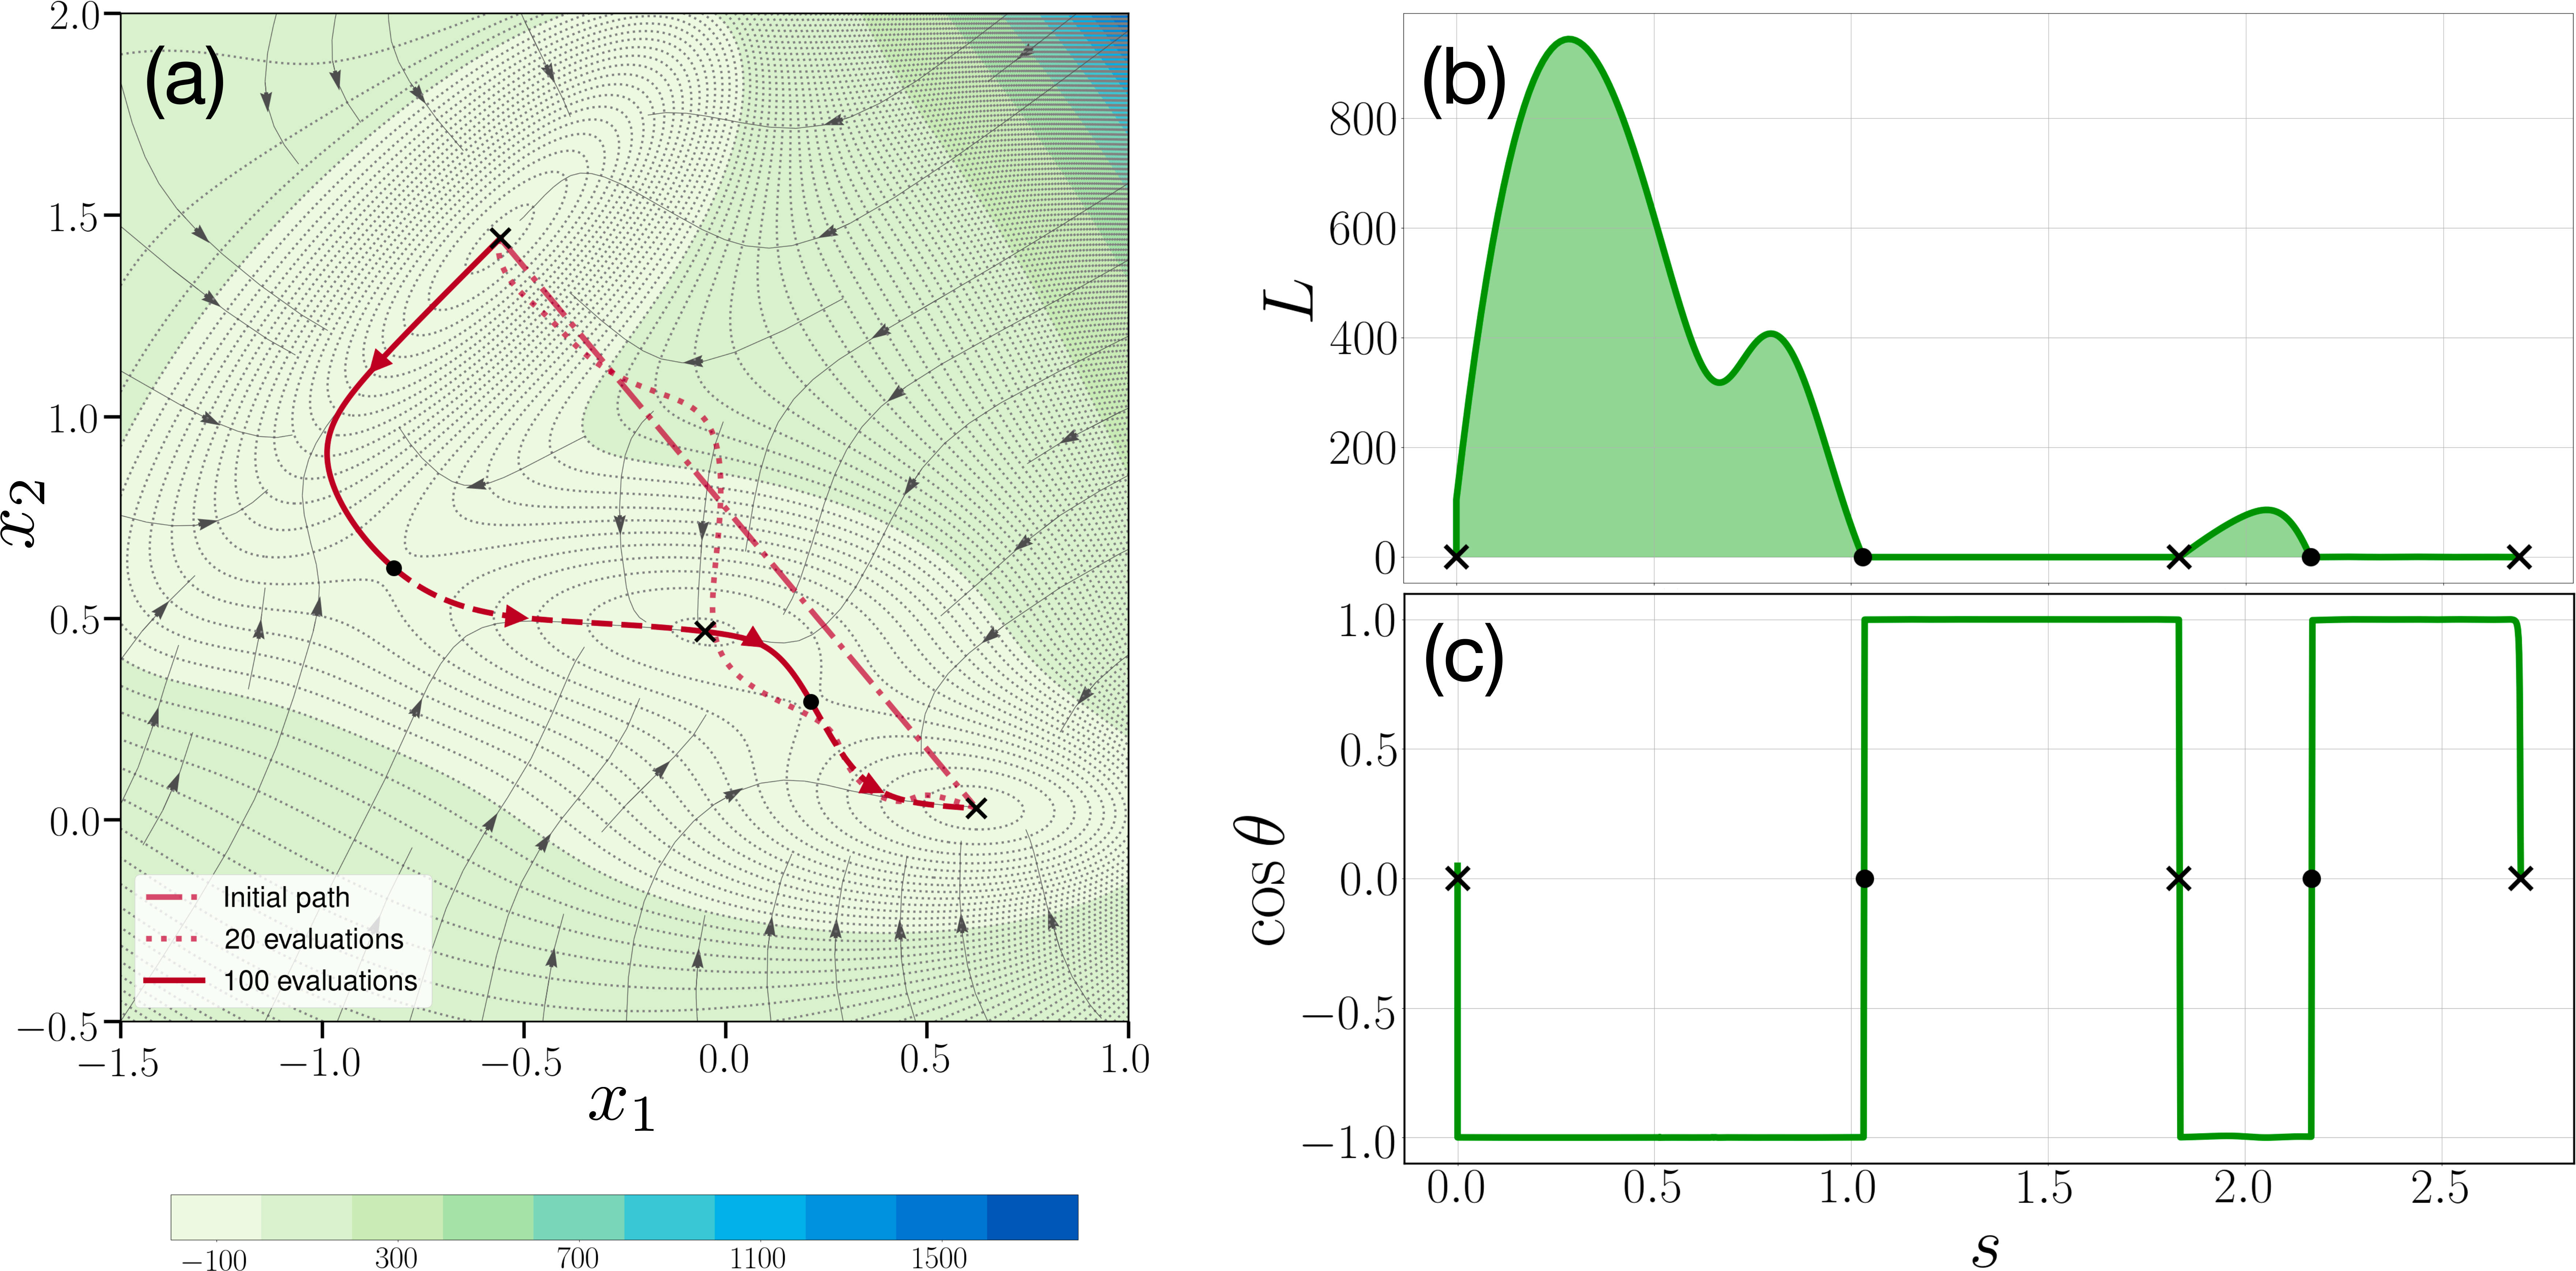
\includegraphics[width=0.94\linewidth]{figs_part1/pyritz/fig1.jpeg}
\par\end{centering}
\caption{Ritz method for overdamped motion in the Müller-Brown potential, which
has three minima (crosses) and two saddle points (dots). The initial
path is the straight line connecting two minima and the instanton
is the solid line, with broken segments showing motion along the force.
The instanton automatically locates and passes through both saddles.
A typical path before convergence to the minimum is shown as a dotted
line. (b) The value of the Lagrangian as a function of Euclidean arc-length
of the instanton. The action vanishes to machine precision on segments
of the path where motion is along the force. (c) The cosine of the
angle $\theta$ between the tangent and the force is always $\pm1$,
i.e. the instanton is a minimum energy path. The instanton is represented
by a polynomial of degree $n=10$. }

\label{fig:muller-brown-instanton}
\end{figure*}


\subsection{Brownian dynamics in a complex potential}

Our first example considers the overdamped Brownian motion in a two-dimensional
potential with a constant friction. The usual equations of Brownian
dynamics can be recast into Itô form,

\begin{align*}
dX_{1} & =-\mu\partial_{1}Udt+\sqrt{2\mu\varepsilon}\,dW_{1}\\
dX_{2} & =-\mu\partial_{2}Udt+\sqrt{2\mu\varepsilon}\,dW_{2},
\end{align*}
where $\mu$ is the mobility and $\varepsilon=k_{B}T$ is the temperature.
The Freidlin-Wentzell action for a smooth path with two-dimensional
coordinate $x=(x_{1},x_{2})$ is
\[
S[x]=\frac{1}{2}\int_{0}^{T}\frac{1}{2\mu}|\dot{x}+\mu\nabla U|^{2}dt
\]
where $\nabla U=(\partial_{1}U,\partial_{2}U)$. The minimum of the
zero-energy action, 

\[
S_{0}[x]=\int_{-1}^{1}|\nabla U(x)||x'|du+\left[U(x)\right]_{-1}^{1},
\]
provides the most probable shape and the stationary quasipotential.
\textcolor{black}{The second term does not affect the minimisation
and can be discarded. The resulting reduced action}

\textcolor{black}{
\begin{equation}
\tilde{S}[x]=\int_{-1}^{1}|\nabla U||x'|du\label{eq:fermat}
\end{equation}
is of the same form as Fermat's principle for optical rays, where
$|\nabla U(x)|$ plays the role of the refractive index and $|x'|du=ds$
is the arc-length of the ray. In geometric optics, Fermat's principle
is equivalent to Huygen's principle and its ``wavelet equation''}

\textcolor{black}{
\begin{equation}
\partial_{i}U=|\nabla U|\frac{dx_{i}}{ds}.\label{eq:huygen}
\end{equation}
}This can be easily verified by differentiatiating it with respect
to arc-length, to obtain the eikonal equation

\textcolor{black}{
\[
\partial_{i}|\nabla U|=\frac{d}{ds}\left[|\nabla U|\frac{dx_{i}}{ds}\right],
\]
which is identical to the Euler-Lagrange equation of the zero-energy
action. The wavelet equation implies that the tangent $t=dx/ds$ to
the path is parallel to the gradient of the potential, or equivalently,
that rays are normal to contours of the potential. This is the well-known
condition for a minimum energy path and was first derived variationally
from the scalar work functional by Olender and Elber \citep{olender1997yet}.
It provides a stringent test of the fidelity of the paths }obtained
by minimisation. 
\begin{figure*}
\begin{centering}
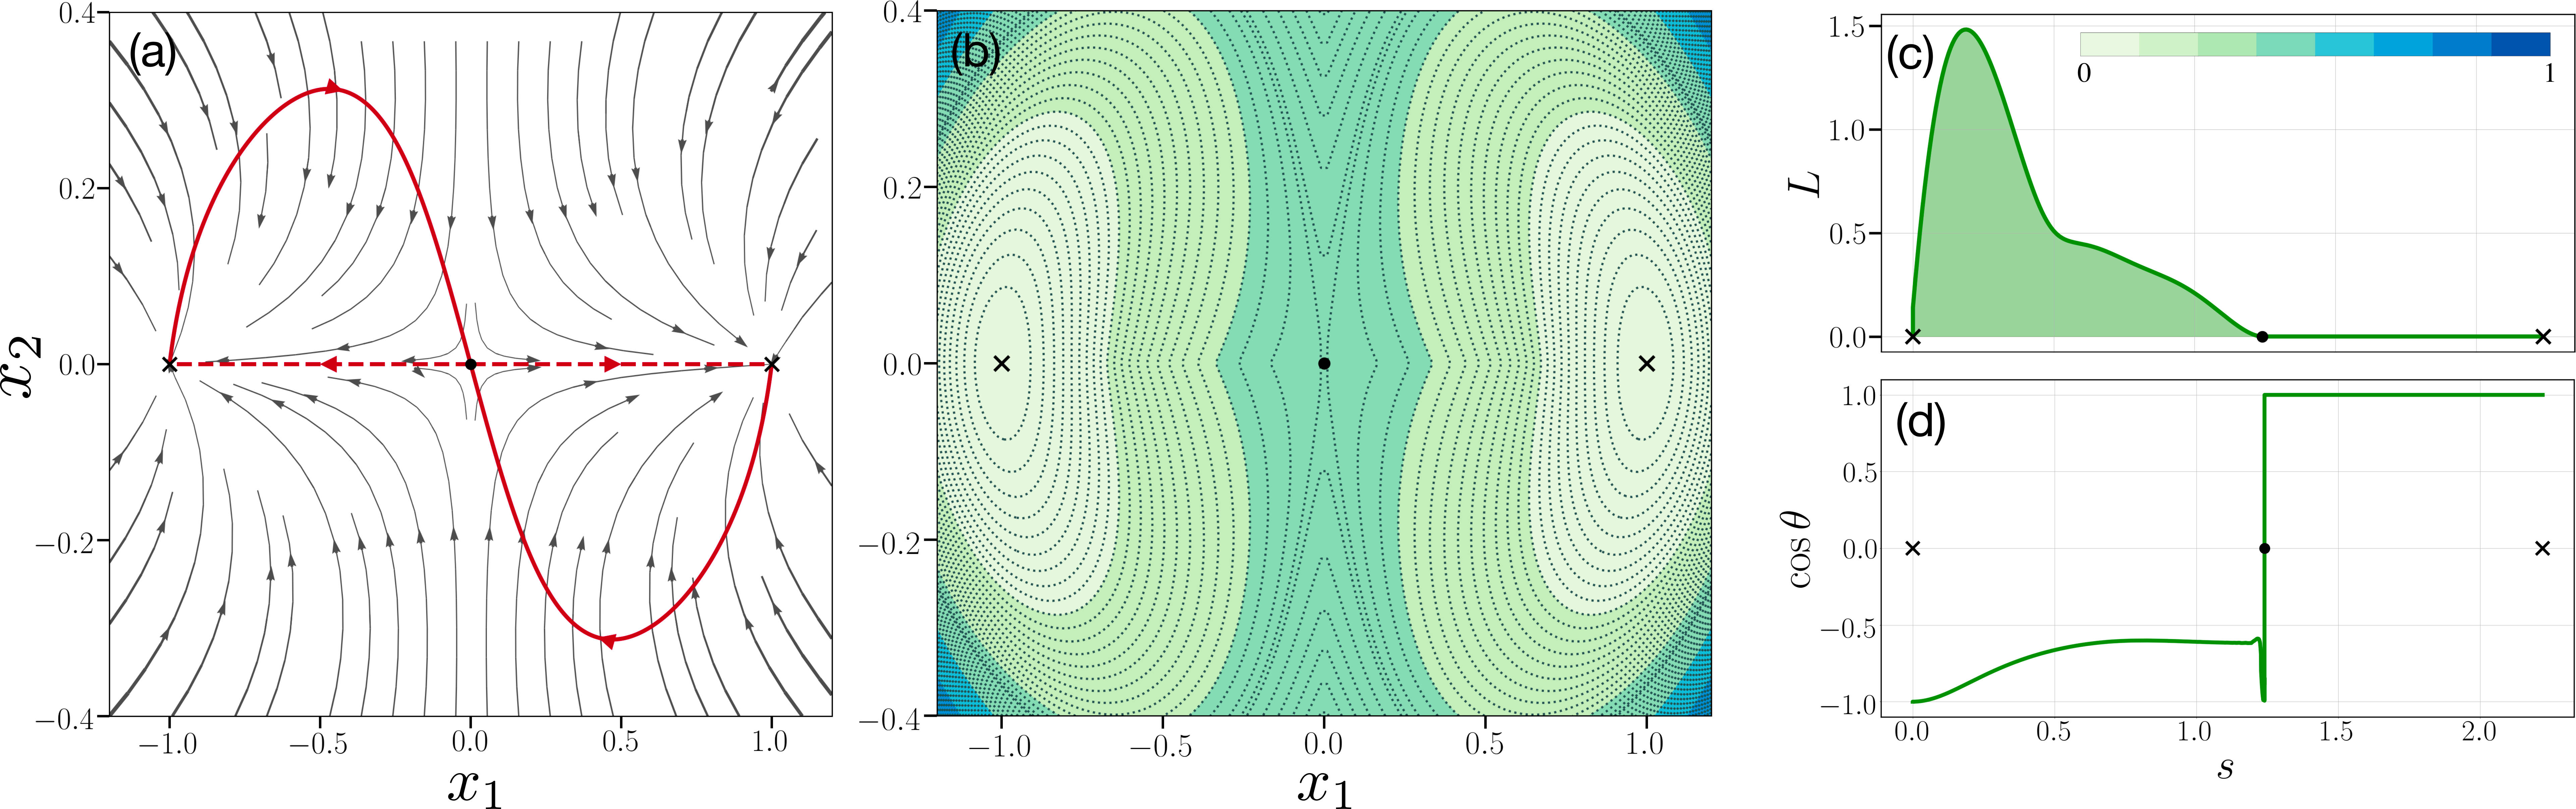
\includegraphics[width=0.99\textwidth]{figs_part1/pyritz/fig2.jpeg}
\par\end{centering}
\caption{Ritz method for overdamped motion in a circulatory (i.e. non-gradient)
force field. The instanton is in red with solid (dashed) segments
showing motion against (along) the force field. The instanton is reflected
about the horizontal axis for motion starting on the right, showing
the inequivalence of fluctuational and relaxational paths for non-gradient
dynamics. (b) The quasipotential, computed using Eq.~\ref{eq:aggregated quasi-potential},
with a caustic at the unstable fixed point. (c) The value of the Lagrangian
as a function of the Euclidean arc-length of the instanton. As in
the potential case, the action vanishes to machine precision on segments
where motion is along the force. (d) The cosine of the angle $\theta$
between the tangent and the force is, unlike in the potential case,
not always $\pm1$. The instanton is represented by a polynomial of
degree $n=8.$ }

\label{fig:maier-stein-quasipotentials}
\end{figure*}

Following \citep{olender1997yet}, we choose the Müller-Brown potential
of \citep{muller1979location} as an example of a complex energy landscape.
The potential and its stationary points are shown in Fig. \ref{fig:muller-brown-instanton}.
The three minima are marked by crosses and two saddle points by dots.
The instanton is computed by requiring the path to start at the minimum
on the top left and terminate at the minimum on the bottom right.
The initial straight line shape, an intermediate shape and the converged
instanton are shown in panel (a). The minimisation automatically locates
the two saddle points and makes the the instanton pass through them.
The action cost along the path is shown in panel (b), where the vanishing
of the action on segments of the path along the force is clearly seen.
The cosine of the angle between the tangent and force is shown in
panel (c) and the condition for a minimum energy path is clearly fulfilled.
We emphasise that the condition is not imposed separately but is satisfied
automatically at the minimum. The Ritz method provides an alternative
to chain-of-states methods for finding minimum energy paths. It does
not need the Hessian of the potential, which makes it suitable for
problems where such evaluations are expensive. Unlike \citep{heymannGeometricMinimumAction2008a},
our parametrisation has no unit-speed constraint and the minimisation,
accordingly, is unconstrained. The method applies without change to
dynamics with configuration-dependent friction. 


\subsection{Brownian dynamics in a circulatory field}

For our second example we consider, in contrast to the first, Brownian motion
in a force field that cannot be derived from a potential and, as such,
necessarily has a non-vanishing curl. Choosing the force field of
Maier and Stein \citep{maier1996scaling} gives

\[
\begin{aligned}dX_{1}= & (X_{1}-X_{1}^{3}-\beta X_{1}X_{2}^{2})dt+\sqrt{\epsilon}dW_{1}\\
dX_{2}= & -(1+X_{1}^{2})X_{2}dt+\sqrt{\epsilon}dW_{2}
\end{aligned}
\]
for the overdamped motion of the two-dimensional coordinate $X=(X_{1},X_{2})$,
where $\beta$ is a parameter. The force field $f(x_{1},x_{2})=(x_{1}-x_{1}^{3}-\beta x_{1}x_{2}^{2},-(1+x_{1}^{2})x_{2})$
is smooth, and $f_{1}$ is odd in $x_{1}$ and even in $x_{2}$, while
for $f_{2}$ the converse holds. There are two stable fixed points
at $x_{a}=(-1,0)$ and $x_{b}=(1,0)$, and a saddle point at $x_{s}=(0,0)$.
The force field admits a potential only for $\beta=1$, when it can
be written as $f=-\nabla U$, with $U(x_{1},x_{2})=-\frac{1}{2}x_{1}^{2}+\frac{1}{4}x_{1}^{4}+\frac{1}{2}(1+x_{1}^{2})x_{2}^{2}$.
The force field is shown in the first panel of Fig. \ref{fig:maier-stein-quasipotentials}
for $\beta=10$ together with the instanton moving from $x_{a}$ to
$x_{b}$. As before, solid (dashed) segments represent motion against
(along) the vector field. The instanton moving from $x_{b}$ to $x_{a}$
is obtained by reflection about the $x_{1}$-axis showing that that
fluctuational and relaxational paths are not identical in a non-gradient
field. 

The middle panels shows the stationary quasipotential $V_{\infty}^{\mathcal{A}_{i}}(x)$
with respect to the attractors at $(-1,0)$ and $(1,0)$ respectively.
The quasipotential is sampled on a $128\times128$ grid by computing
instantons between a point on the grid and the relevant attractor.
The contours of the quasipotential and its heatmap are obtained from
these discrete samples. To the best of our knowledge, all prior estimations
of the quasipotential for this problem (and more generally, for circulatory
forces) have required numerical solutions of the Hamilton-Jacobi equation.
Our method of direct sampling provides an alternative to this route
of computing the quasipotential. The right panel shows the Lagrangian
as a function of arc-length along the instanton. As in the previous
example, the Lagrangian vanishes along segments of the path where
motion is along the force. For motion against the force, the tangent
to the path is no longer parallel to the force, as shown by the variation
of the cosine of the angle $\theta$ between the tangent and the force.
We note that our method is agnostic to the existence, or not, of a
potential for the drift and treats both these cases on equal footing.


\subsection{Multistability in a genetic switch system}

We continue with the dynamics of a two-dimensional coordinate $x=(x^{1},x^{2})$
in a non-gradient field, but now of non-mechanical origin and non-polynomial
form,

\begin{equation}
\begin{aligned}dx^{1} & =\left(\frac{a_{1}}{1+\left(\frac{x^{2}}{K_{2}}\right)^{n}}-\frac{x^{1}}{\tau}\right)dt+\sqrt{\epsilon}dW^{1}\\
dx^{2} & =\left(\frac{a_{2}}{1+\left(\frac{x^{1}}{K_{1}}\right)^{m}}-\frac{x^{2}}{\tau}\right)dt+\sqrt{\epsilon}dW^{2},
\end{aligned}
\label{eq:genetic-switch}
\end{equation}
where $a_{1},$ $a_{2}$, $\tau$, $n$, $m$, $K_{1}$ and $K_{2}$
are constants. This model is due to Roma \emph{et al} \citep{roma2005optimal}
and describes a multistable genetic network. In the region of configuration
space we consider, the vector field has two fixed points one of which
is stable and the other a saddle. The top panel of Fig. \ref{fig:genetic-switch-quasipotential}
shows the instantons moving between these fixed points. Unlike in
the previous examples, here the instantons move either entirely with
(solid line) or entirely against (dashed line) the flow. The bottom
panel shows the quasipotential with respect to the stable fixed point.
The procedure to evaluate and plot it is as described above. The quasipotential
provides a quantification of the dispersion of the coordinate about
the stable fixed point and a measure of the non-equilibrium ``temperature''
on the state-space of this non-mechanical system. 

\begin{figure*} 
    \centering
     
    \begin{subfigure}[b]{0.4\textwidth}  
        \centering 
        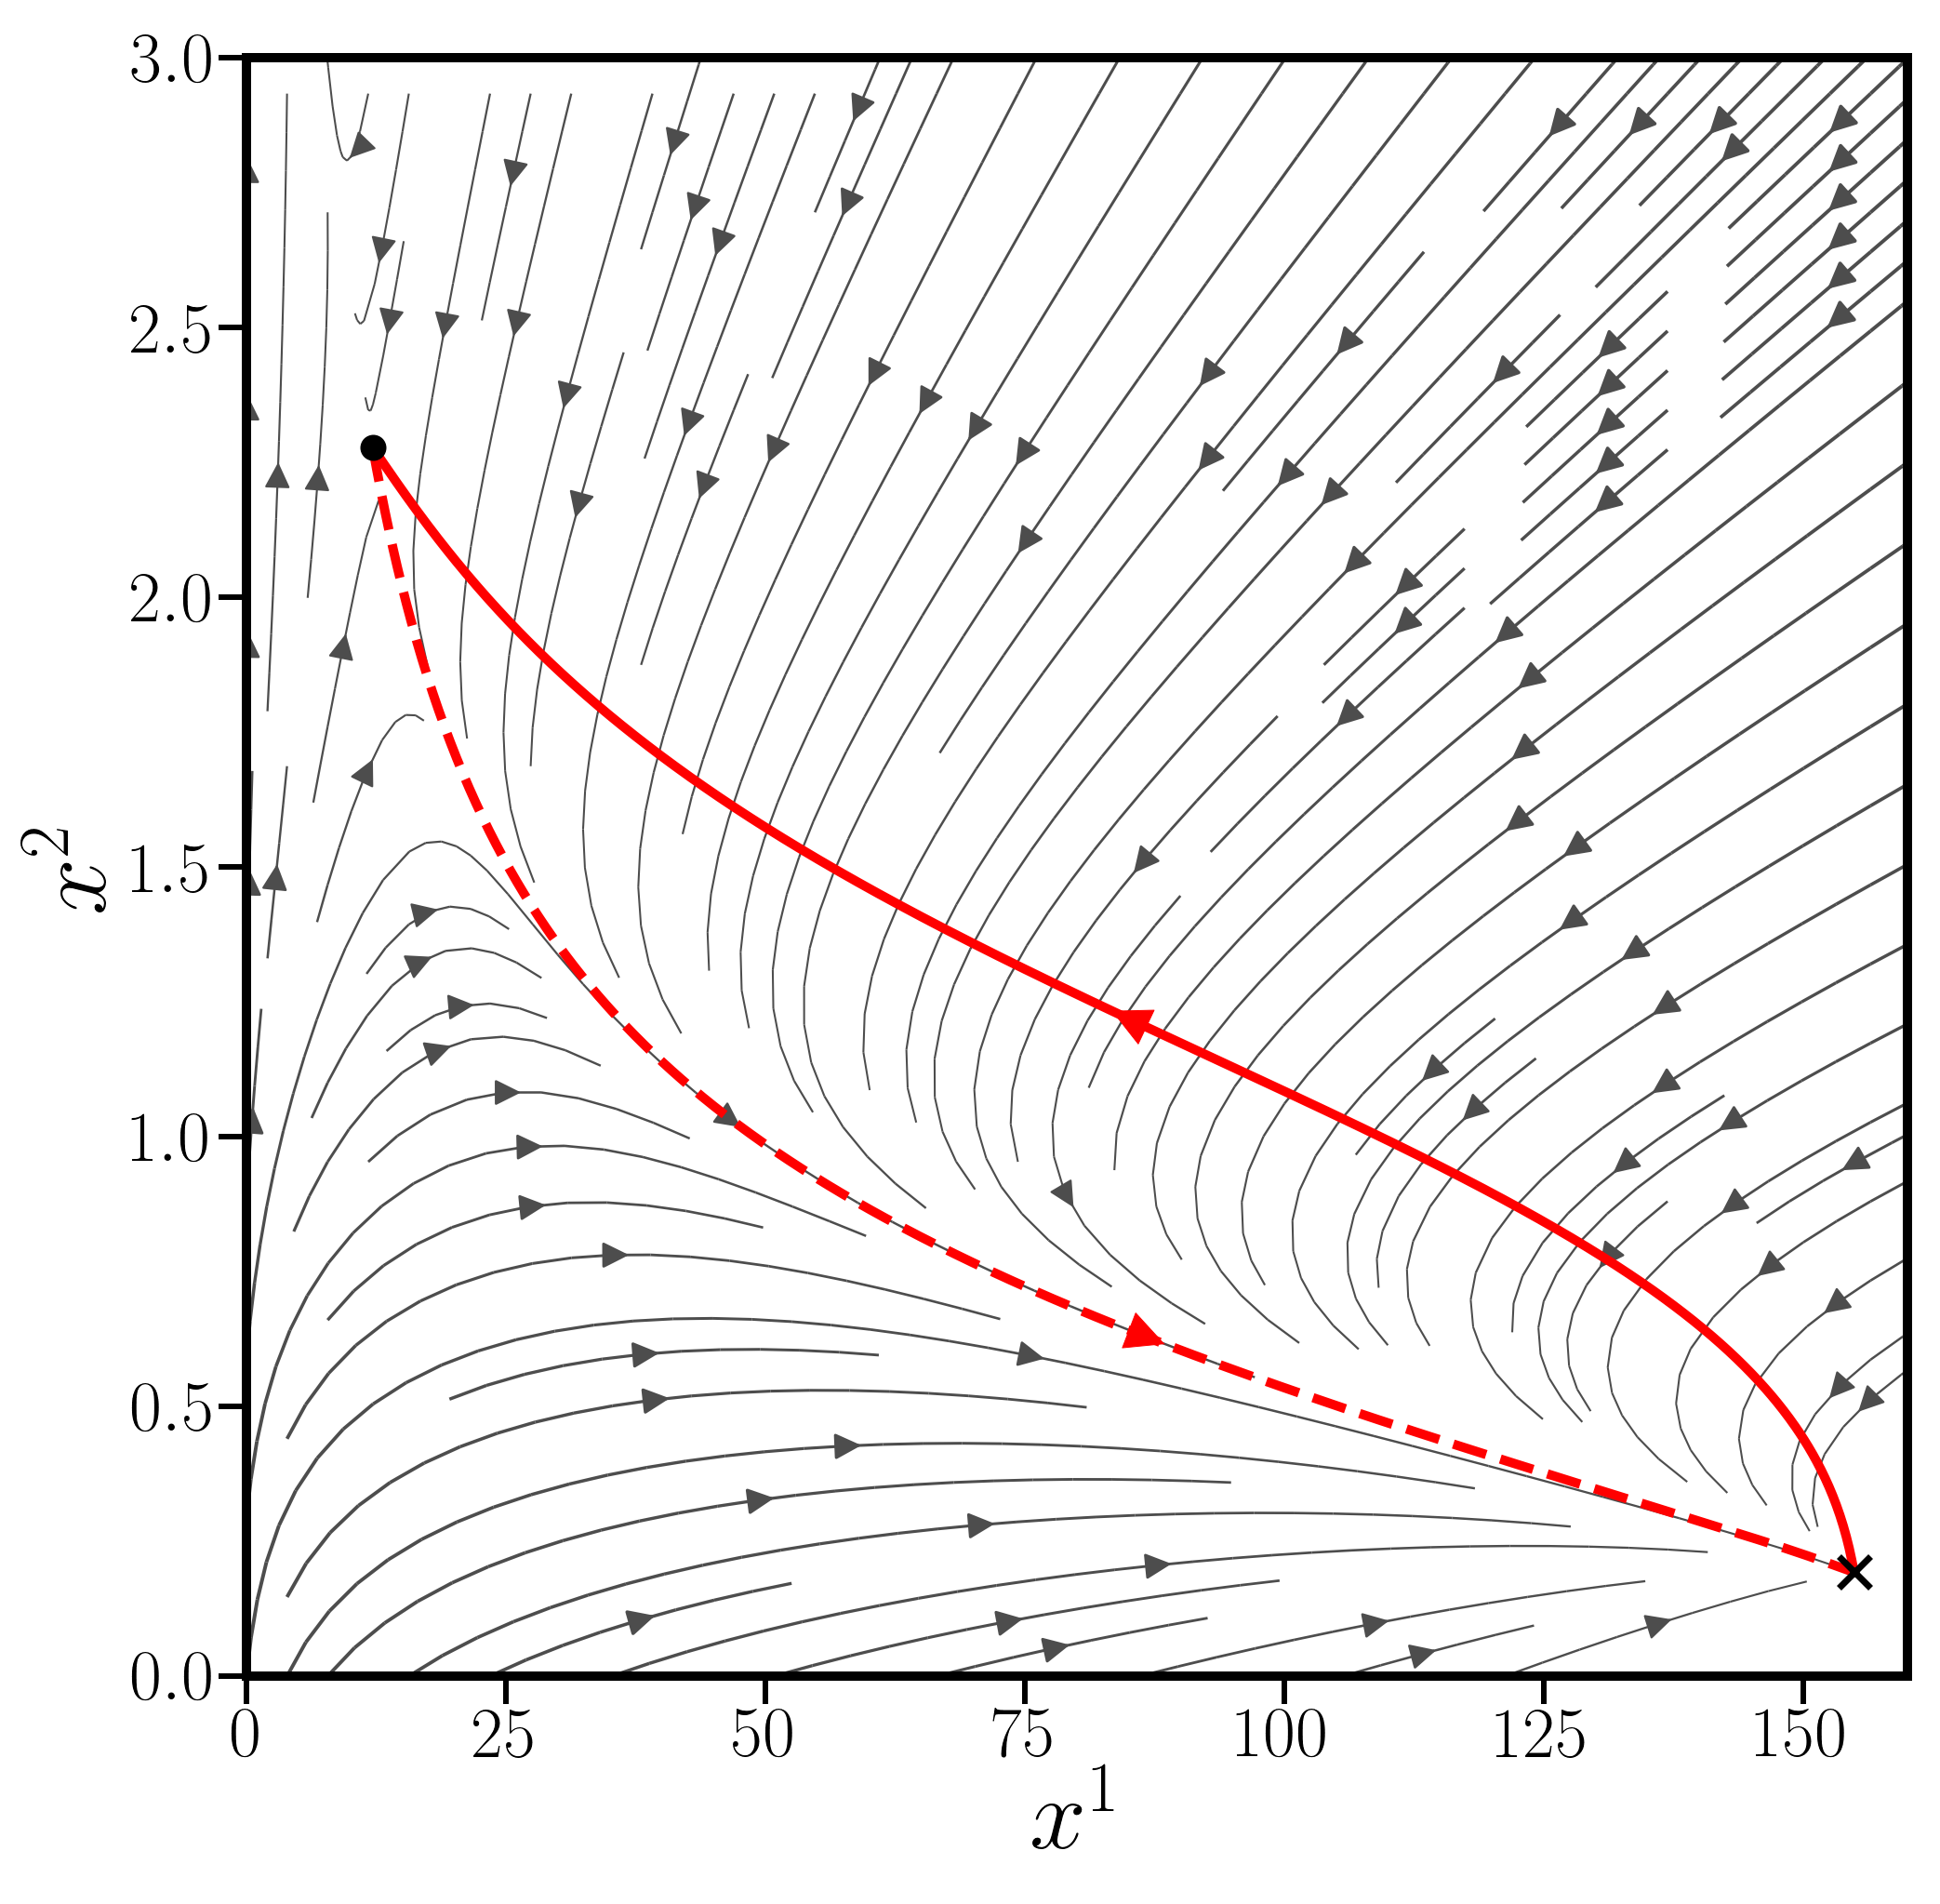
\includegraphics[width=\textwidth]{figs_part1/pyritz/genetic_switch_instanton.png}
        \caption[]%
        {}    
        \label{fig:genetic switch inst}
    \end{subfigure}
    \hspace{0.4cm}
    \begin{subfigure}[b]{0.4\textwidth}
        \centering
        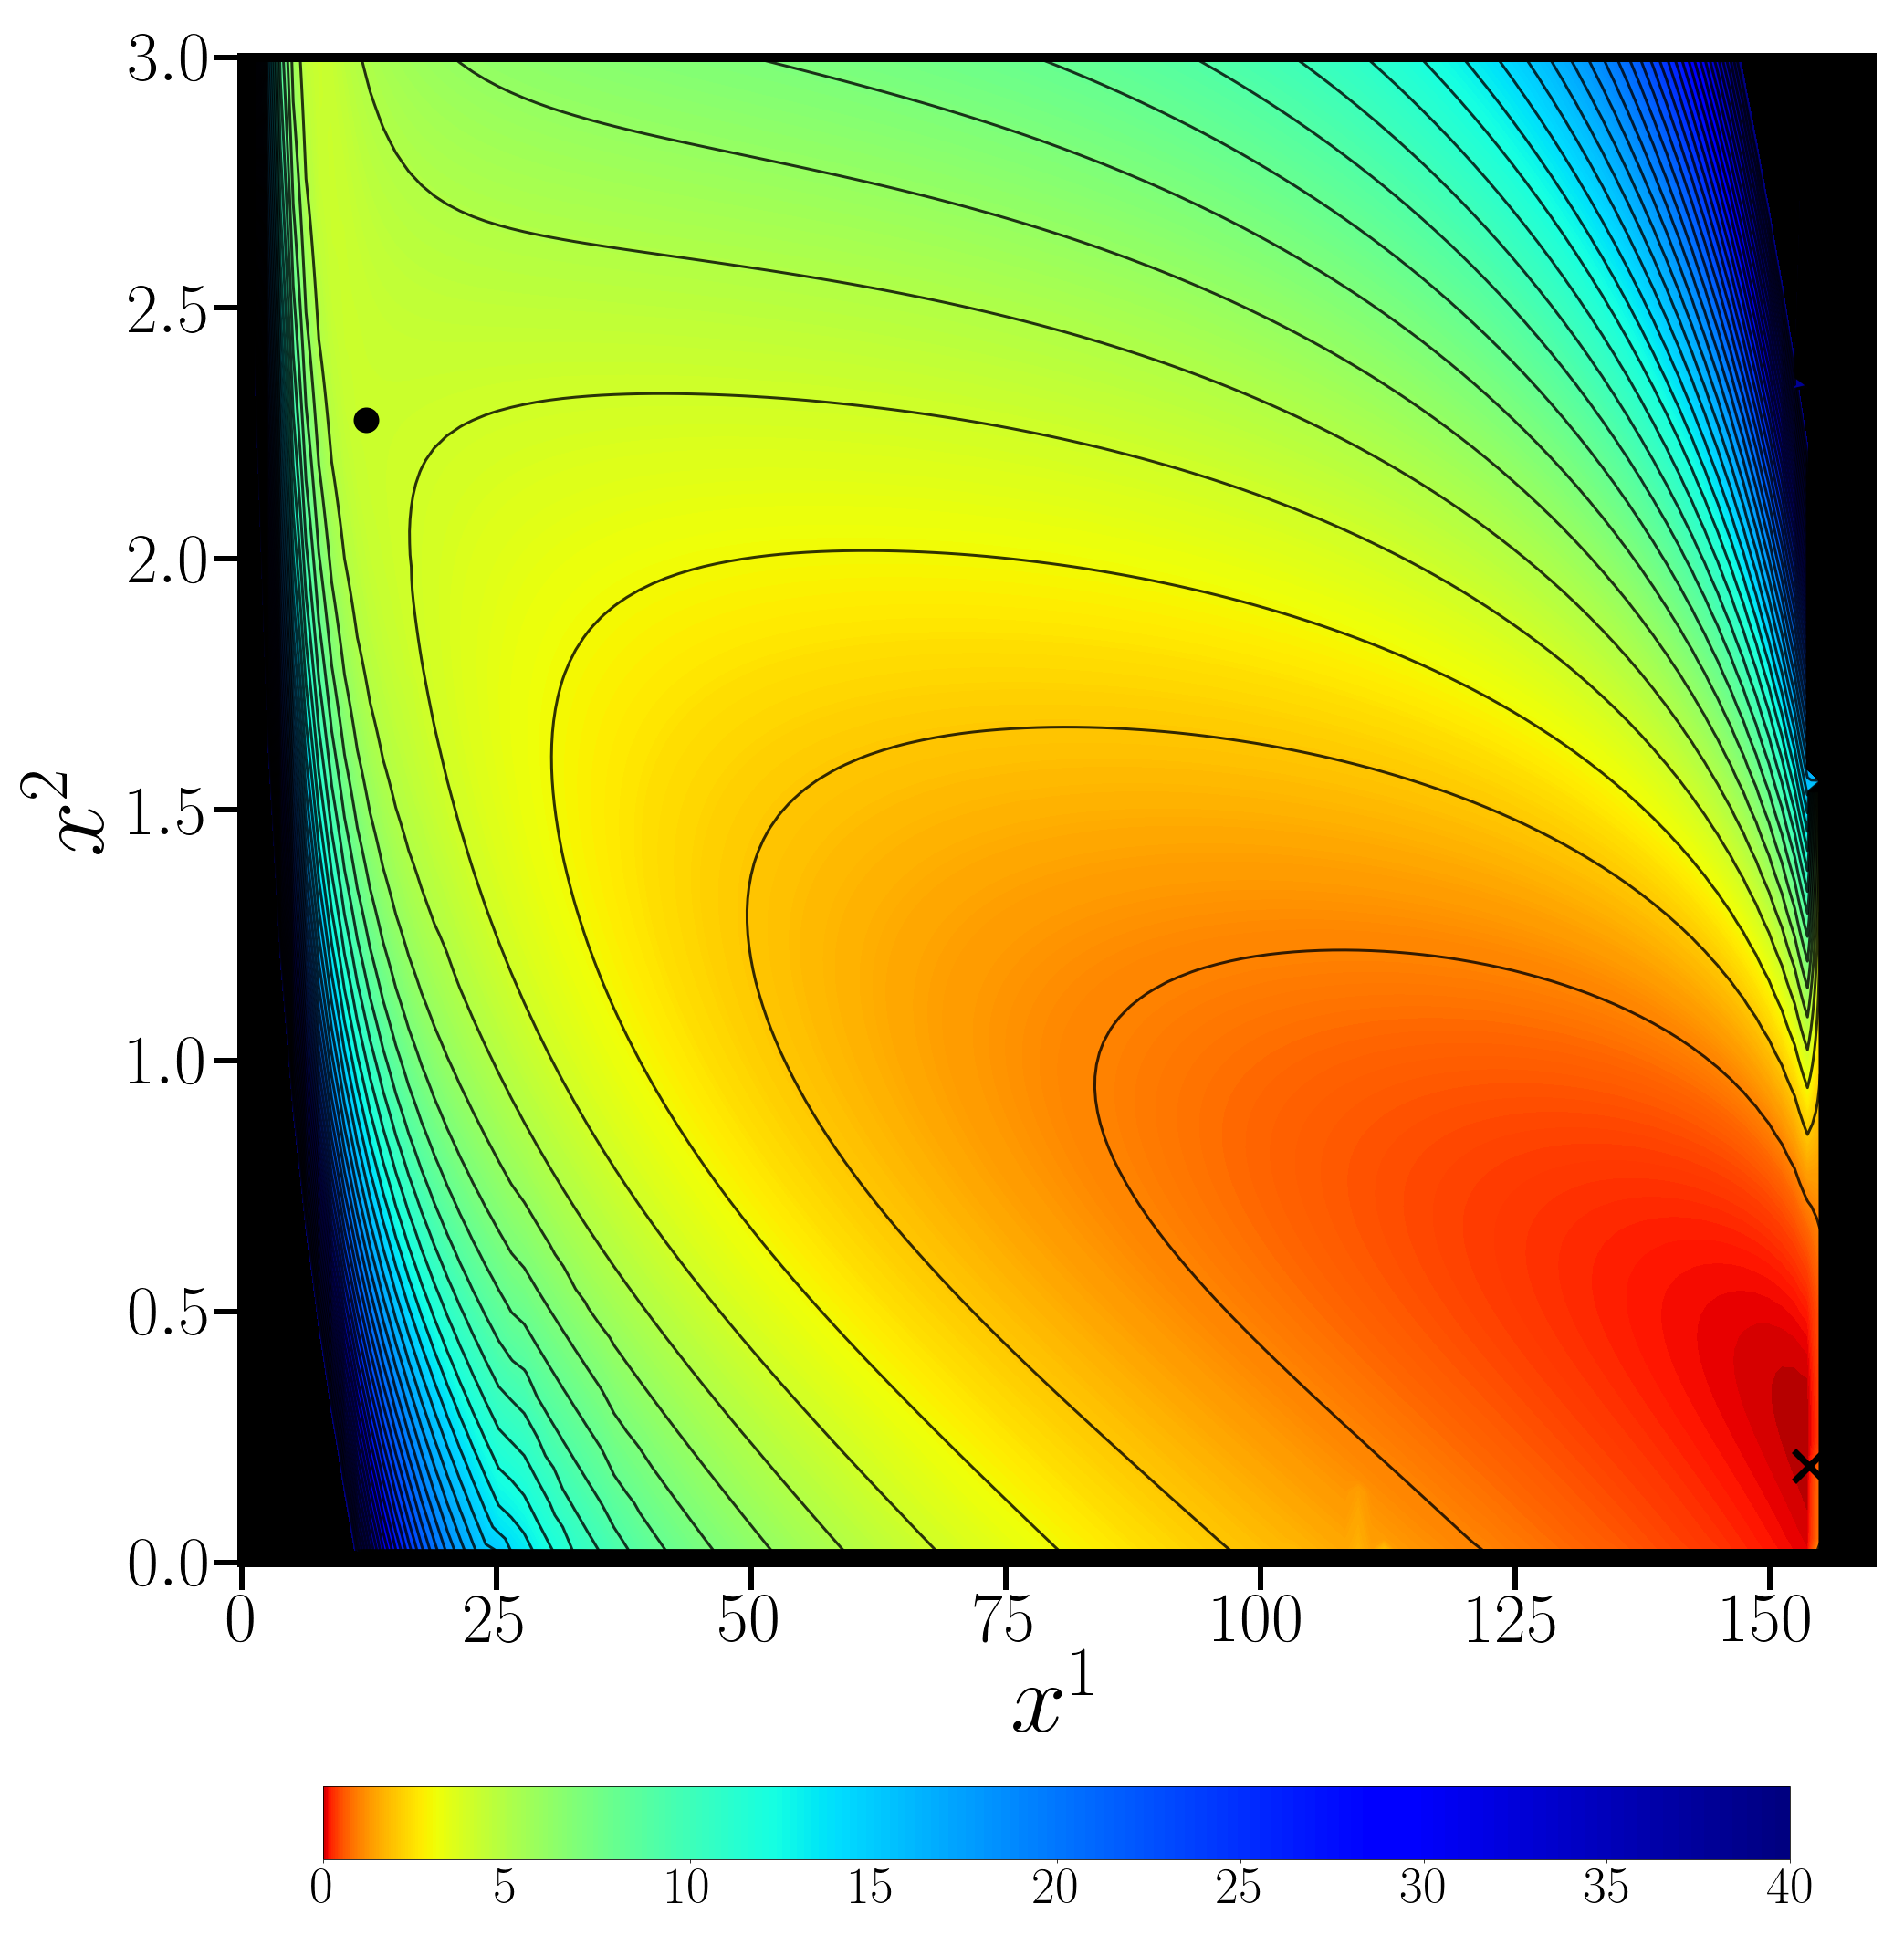
\includegraphics[width=\textwidth]{figs_part1/pyritz/genetic_switch_quasipotential_from_xb_to_xa.png}
        \caption[Extending Cosserat rod]%
        {}    
        \label{fig:genetic switch quasi}
    \end{subfigure}    
    \caption[ ]
    {\small Instantons for the genetic switch. (a) shows the instantons
in red with solid (dashed) lines representing motion against (along)
the vector field. (b) shows the quasipotential with respect
to the stable fixed point (cross). Parameter values are $a_{1}=156$, $a_{2}=30$,
$\tau=1$, $n=3$, $m=1$ and $K_{1}=K_{2}=1$. A polynomial of degree $n=10$ was used to parametrise the path.} 
    \label{fig:genetic-switch-quasipotential}
\end{figure*} 



\subsection{Transitions between limit cycles}

To demonstrate that our method is not limited to fixed points, we
constructed a simple but non-trivial system:

\begin{equation}
\begin{aligned}dr & =(1+\cos^{2}\theta)f(r)dt+dW^{r}\\
d\theta & =r(1+\sin^{2}\theta)dt+dW^{\theta}
\end{aligned}
\label{eq:limit-cycle system}
\end{equation}
where $f(r)=-\frac{1}{4}r(r-s_{1})(r-s_{2})(r-s_{3})$, and $s^{(i)}=[1,3,5]$.
We have an unstable fixed point at $r=0$, stable limit cycles at
$r=s_{1}$ and $r=s_{3}$, and an unstable limit cycle at $r=s_{2}$.
The trigonometric factors in the drift breaks the circular symmetry
of the system, but preserves the concentric circular limit cycles.
We consider instantons moving from the inner stable limit cycle $r=s_{1}$
to the outer limit cycle $r=s_{3}$. Let $\Gamma_{i}=\{(r,\theta)\,|\,r=s_{i}\}$
for $i=1,2,3$, be the set of points comprising the three limit cycles.
For a given path $x(t)$, let $x_{i}\in\Gamma_{i}$ be the points
along the path located along the respective limit cycles. Since $a_{r}(x_{i})=0$
and $a_{\theta}(x)$ is positive definite, the system can move to
any point within a limit cycle without incurring any action cost.
Therefore the starting, intermediate and end points $x_{1}$, $x_{2}$
and $x_{3}$ should be varied freely within their respective limit
cycles during the minimisation. We can split the instanton $x^{*}(t)$
into an ``uphill'' path $x_{\uparrow}^{*}(t)$, moving between $\Gamma_{1}$
and $\Gamma_{2}$, and a ``downhill'' path $x_{\downarrow}^{*}(t)$,
moving between $\Gamma_{2}$ and $\Gamma_{3}$. The downhill path
follows deterministic relaxational dynamics, and does not contribute
to the action, and therefore the only non-trivial part of the problem
is the uphill path $x_{\uparrow}^{*}(t)$. One issue with limit cycle
problems is that instantons in general have infinite arc-lengths.
In the case of the relaxational path $x_{\downarrow}^{*}(t)$, this
can be verified to be the case using an ODE solver. The system will
not only relax to the attractor in infinite time, but the system will
also undergo an infinite number of cycles before reaching the stable
limit cycle $\Gamma_{3}$. We would expect similar behaviour for diffusive
paths leaving stable limit cycles. Paths of infinite Euclidean arc-length
are not possible to parametrise exactly in the Chebyshev basis, so
only an approximate finite-length instanton can be found, as shown
in Fig. \ref{fig:concentric}. As we increased the arc-length the action of the candidate instanton converged to a value of $S\approx3.65053$.
\begin{figure}[t]
\begin{centering}
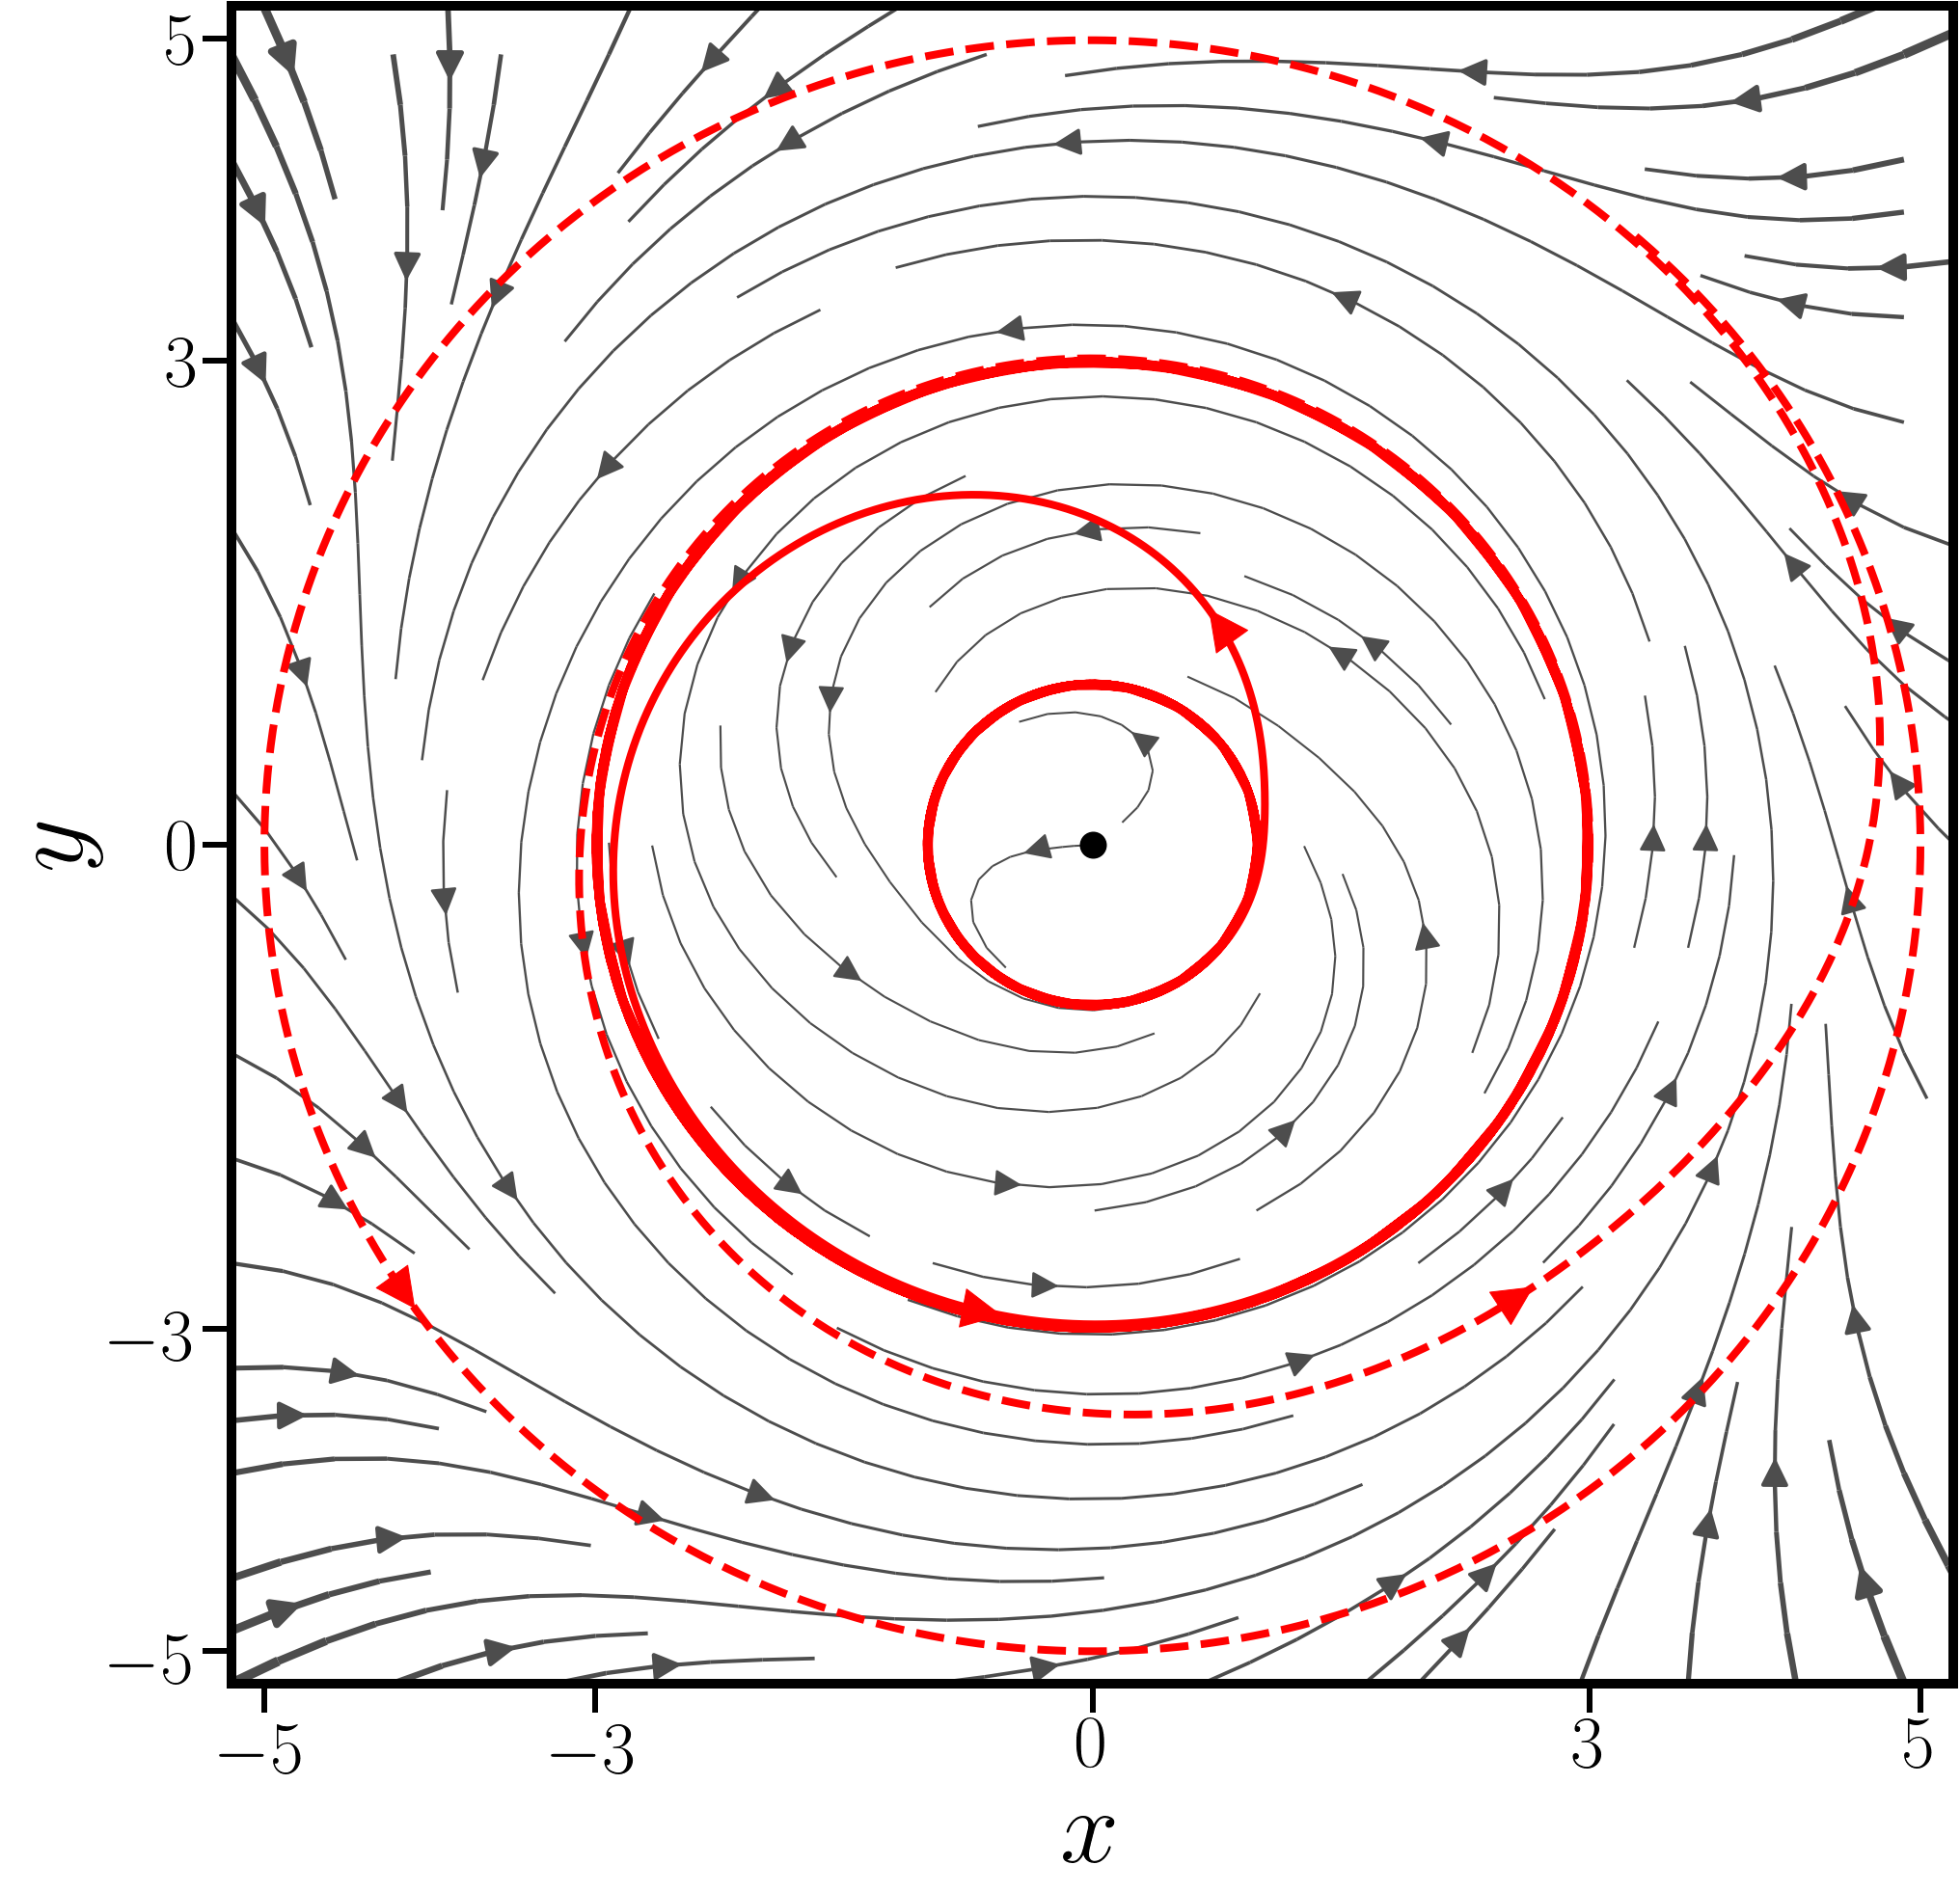
\includegraphics[width=0.7\columnwidth]{figs_part1/pyritz/concentric_limit_cycle_instanton.png}
\par\end{centering}
\caption{An approximate instanton of the concentric limit cycle system with $S\approx3.65053$.
The instanton moves from the inner stable limit cycle at $r=1$ to the unstable limit cycle at $r=3$, and then moves hetero-clinically along the drift to the outer stable limit cycle at $r=4$.}
\label{fig:concentric}
\end{figure}

\subsection{Egger model of weather}

\begin{figure*}
\begin{centering}
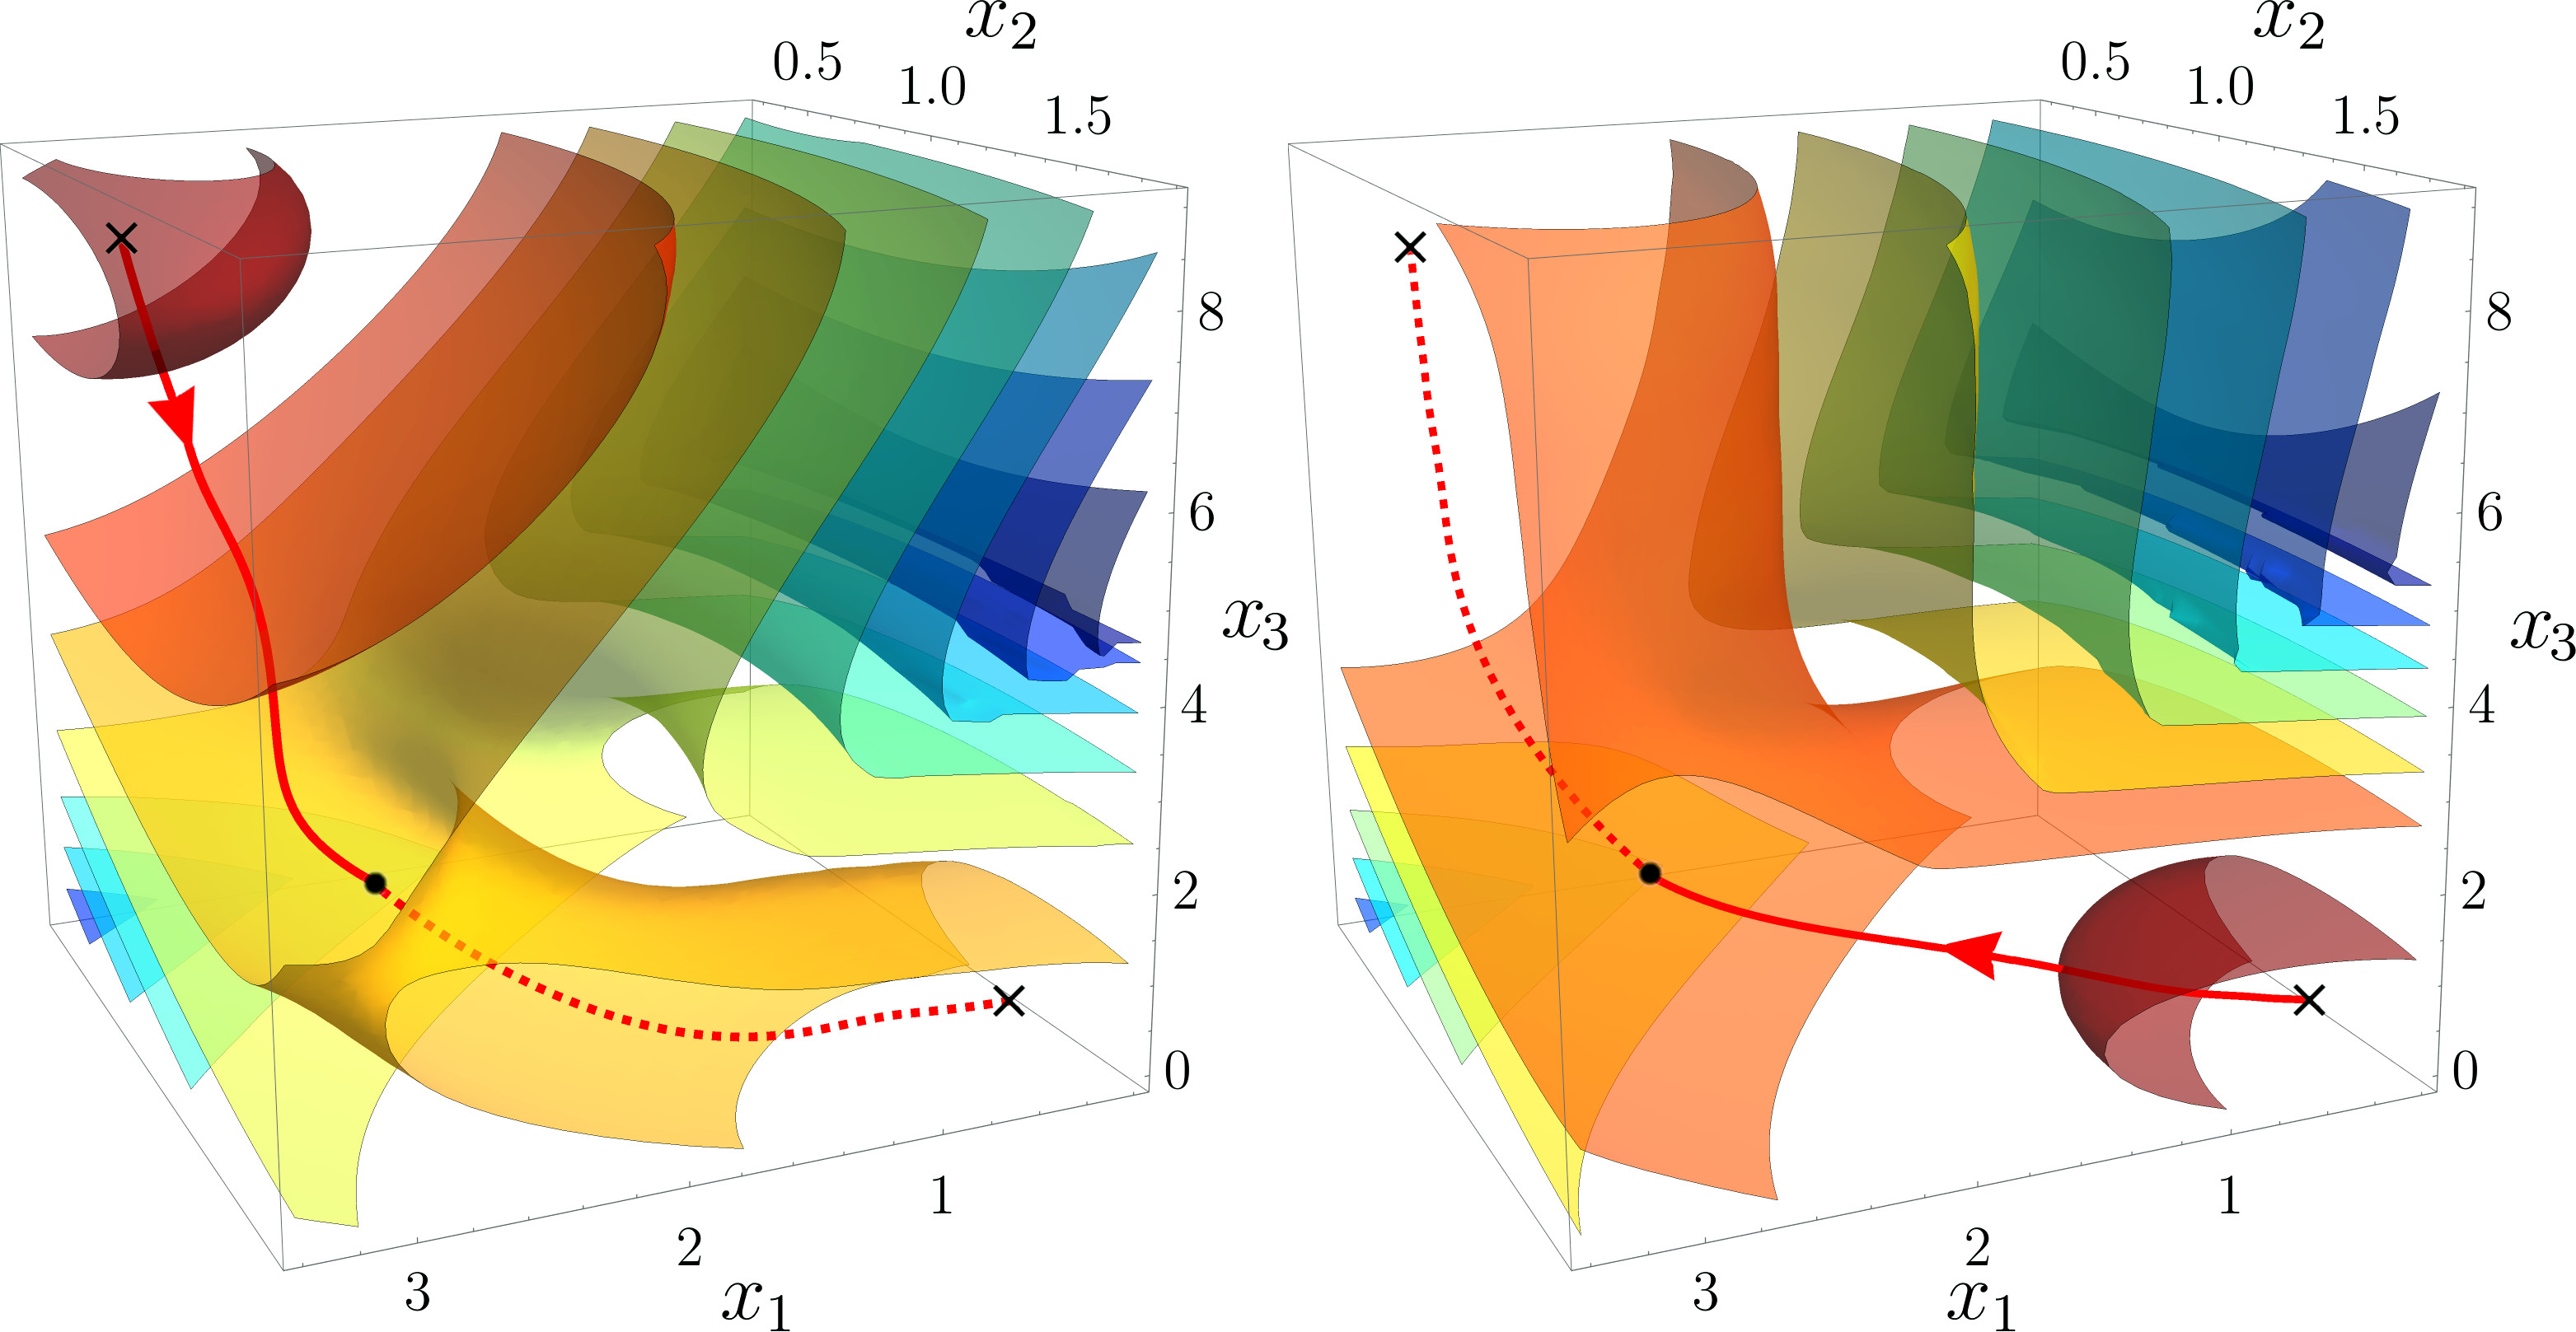
\includegraphics[width=0.9\textwidth]{figs_part1/pyritz/fig3.jpeg}
\par\end{centering}
\caption{Instantons and quasi-potentials of the Egger model. The instantons
are shown in red with solid (dashed) lines representing motion against
(along) the vector field. The left and right panels are forward and
reverse instantons. Isosurfaces of the quasipotential with respect
to each attractor is shown in the respective panels. Isovalues increase
from light red to blue in the range $\left\{ 1,7,11,16,21,26,31,36\right\} $.
Parameter values are $k=2$, $\beta=1.25$, $\gamma=2$, $U_{0}=10.5$
and $H=12$. The instanton is represented by a polynomial of degree
$n=10.$}
\centering{}\label{fig:eggers}
\end{figure*}

Our final example is a reduced model of the weather for a a three-dimensional
coordinate $X=(X_{1},X_{2},X_{3})$ that has a circulatory drift,
\begin{alignat}{1}
dX_{1}= & \left[kX_{2}\left(X_{3}-\frac{\beta}{k^{2}}\right)-\gamma X_{1}\right]dt+\sqrt{\epsilon}dW_{1}\nonumber \\
dX_{2}= & \left[kX_{1}\left(\frac{\beta}{k^{2}}-X_{3}\right)-\gamma X_{2}+\frac{HX_{3}}{k}\right]dt+\sqrt{\epsilon}dW_{2}\nonumber \\
dX_{3}= & \left[-\tfrac{1}{2}HkX_{2}-\gamma(X_{3}-U_{0})\right]dt+\sqrt{\epsilon}dW_{3}\label{eq:egger}
\end{alignat}
where $k$, $\beta$, $\gamma$, $U_{0}$ and $H$ are constants.
This model is due to Egger \citep{egger1981stochastically}. It is
not particularly illuminating to visualise the three-dimensional vector
field describing this dynamics but we note that it has two stable
fixed points, marked by crosses in Fig. \ref{fig:eggers}, and a saddle
fixed point marked by a dot. The instanton moving between these points
is shown as before in the left and right panels of the figure. Also
shown are isosurfaces of the quasipotential with respect to the stable
fixed points, with isovalues increasing from red to blue. To the best
of our knowledge, this is the first computation of the quasipotential
for this model. We provide this example primarily to demonstrate the
feasibility of sampling quasipotentials in dimensions greater than
two with our method. 

\setlength{\tabcolsep}{2.5pt}

\begin{table}
\begin{centering}

\begin{tabular}{|c|c|c|c|c|c|}
\hline 
Model & $S_{1}-S_{2}$ & $S_{3}-S_{4}$ & $S_{7}-S_{8}$ & $S_{15}-S_{16}$ & $S_{31}-S_{32}$\tabularnewline
\hline 
\hline 
M-B & $2$ & $3\times10^{-4}$ & $1\times10^{-7}$ & $5\times10^{-14}$ & $1\times10^{-13}$\tabularnewline
\hline 
M-S & $2\times10^{-3}$ & $3\times10^{-7}$ & $2\times10^{-12}$ & $1\times10^{-16}$ & $5\times10^{-16}$\tabularnewline
\hline 
Egger & $8\times10^{-3}$ & $1\times10^{-3}$ & $6\times10^{-7}$ & $4\times10^{-9}$ & $8\times10^{-13}$\tabularnewline
\hline 
\end{tabular}%

\vspace{0.2cm}

\begin{tabular}{|c|c|c|c|c|c|}
\hline 
Model & $S_{2}-S_{50}$ & $S_{4}-S_{50}$ & $S_{8}-S_{50}$ & $S_{16}-S_{50}$ & $S_{32}-S_{50}$\tabularnewline
\hline 
\hline 
M-B & $4\times10^{-2}$ & $4\times10^{-5}$ & $8\times10^{-8}$ & $1\times10^{-12}$ & $3\times10^{-13}$\tabularnewline
\hline 
M-S & $2\times10^{-4}$ & $7\times10^{-11}$ & $2\times10^{-13}$ & $1\times10^{-16}$ & $2\times10^{-16}$\tabularnewline
\hline 
Egger & $5\times10^{-3}$ & $1\times10^{-4}$ & $1\times10^{-6}$ & $1\times10^{-8}$ & $2\times10^{-10}$\tabularnewline
\hline 
\end{tabular}

\par\end{centering}
\caption{Convergence of the action $S_{n}$ for a path of polynomial order
$n$. The abbreviations M-B and M-S refer to Brownian dynamics in
the Müller-Brown potential and the Maier-Stein force field respectively.
The first table shows the difference $S_{n}-S_{n+1}$ while
the second table shows the difference $S_{n}-S_{50}$. A tenth-order polynomial
typically gives at least six digits of accuracy. {\label{tab:Convergence}}}
\end{table}

\section{Numerical convergence}

We briefly recall the convergence properties of the Ritz method, comprising
that of the basis functions, the quadrature, and the optimisation.
The Chebyshev interpolant converges to the most probable
path, assuming that it is Lipschitz continuous, at a rate that increases
with the number of derivatives the path admits and is exponential
for a smooth path. Likewise, the Clenshaw-Curtis quadrature is guaranteed
to converge to the minimum of the action, assuming that the Lagrangian
is Lipschitz continuous. The optimal number of quadrature points for
accuracy to machine precision can be obtained by following the decay
of the Chebyshev coefficients of the Lagrangian and truncating at
that value beyond which the coefficients vanish to machine precision.
The optimisation has lesser theoretical guarantees than the interpolation
and quadrature, as is generally the case with search in high-dimensional
spaces. However, the residual of the Ritz system provides an empirical
measure for how closely the minimum has been located. In all three
examples (and in others not presented here) we have found both gradient-free
and gradient-based optimization to robustly locate the minima, and
gradient-based methods to yield faster convergence. We note that for
equilibrium problems, the gradient-free method does not require the
Hessian of the energy function, which can be of significant computational
advantage. In Table \ref{tab:Convergence} we show the spectral convergence
of the action with increasing polynomial order of the path for each
of our examples. 

\section{Conclusion}

We have presented an efficient and accurate numerical method for computing
most probable transitions paths and quasipotentials of rare diffusive
events. The method directly minimises the Freidlin-Wentzell action
and thus provides a unified approach for transition
paths in both equilibrium and non-equilibrium systems. Our reparametrisation-invariant
form of the action, derived using a Noether symmetry, is well-suited
for numerical work and is a generalisation of the geometric action.
This frees us from the constraints of the commonly used arc-length
path parametrisation and offers the maximum flexibility in choosing
the space of polynomials in which action is minimised. Thus our method
is not limited to the Chebyshev polynomials in $[-1,1]$ used here
but easily admits trigonometric polynomials and, more generally, any
global basis. Numerical quadrature reduces the action to a multivariate
function of coefficients of the path polynomial whose minimum is obtained
by both gradient-free and gradient-based optimisation. This gives,
simultaneously, both the minimum value of the action and the most
probable path. This efficiency of the method allows us to repeatedly
compute minimum action paths between an attractor and a point in its
basin of attraction and, thereby, map out the quasipotential. The
quasipotential in a non-equilibrium steady state has the same significance
as the Gibbs distribution in equilibrium and our method provides a
robust way of obtaining it without the need to numerically solve the
Hamilton-Jacobi partial differential equation. 
\begin{figure}
\begin{center}
\begin{tikzcd}[column sep=small, row sep=small]      
& S[x] \arrow{ddl}[swap]{\delta} \arrow{ddr}{\mathcal{P}} &
\\     &  &
\\[2ex]     
\delta S[x]=0  & & S(\alpha) \hspace{0.5cm}
\end{tikzcd}
\end{center}  
\begin{center}
\vspace{-0.6cm}
\begin{tikzcd} 
\arrow{d}[swap]{\mathcal{P}} &     \arrow{d}{\nabla} 
\\[2ex]     
\text{Discrete E-L} & \text{Ritz system} 
\end{tikzcd} 
\end{center}  

%\begin{center}
%\begin{tikzcd} [column sep=small, row sep=small]
%\delta,\nabla,\pi \rightarrow \text{variation, extremization, %projection}
%\end{tikzcd} 
%\end{center}  

\caption{Inequivalence of the direct and Euler-Lagrange routes to numerical
action minimization. Here, $\delta$ $\rightarrow$ functional variation,
$\mathcal{P}\rightarrow$ finite-dimensional projection, and $\nabla\rightarrow$
function minimisation. On the left branch, the action is first varied
to obtain the Euler-Lagrange equation and then projected onto a finite-dimensional
basis for numerical solution. On the right branch, the action is first
projected onto a finite-dimensional basis and then minimised to obtain
the Ritz system. The finite-dimensional projection of the Euler-Lagrange
equations is, in general, not identical to the Ritz system.}

\centering{}\label{fig:discrete-el-versus-ritz}
\end{figure}

The direct method used here consists of a discretisation of the action
followed by a search for the minimum in the resulting finite-dimensional
space, expressed schematically in Fig. (\ref{fig:discrete-el-versus-ritz}).
In contrast, the majority of methods impose the vanishing variation
of the action and then search for the solution of the Euler-Lagrange
equation in a finite-dimensional space. The resulting discretised
Euler-Lagrange equations is, in general, not identical to the Ritz
system; in other words, these two methods of reducing an infinite-dimensional
problem to a finite-dimensional one are not equivalent. In contra st
to mechanics, where Newton's equations of motion are considered primary
and the action derived, here it is the tube probability and hence
the Freidlin-Wentzell action that is primary and the Euler-Lagrange
equation for the most probable path that is derived. It appears more
natural to us to discretise the primary, rather than the derived,
object directly. Our approach is algorithmically simple and the only
adjustable parameters are the polynomial order $n$ and the quadrature
order $n_{q}.$ This simplicity does not compromise accuracy or efficiency,
as confirmed by our examples.  

In subsequent chapters we will move beyond the Freidlin-Wentzell regime, which corresponds to the limit of zero diffusivity and infinite duration, to study transition paths in systems at finite temperatures and of varying durations. In this setting, the Ritz methods developed here can be applied to find finite-temperature instantons of the \textit{Onsager-Machlup action}. Although in this regime the action does not admit a on-shell form, as was the case for the Freidlin-Wentzell action.

%The rapid convergence of the method holds promise for its application
%to problems involving the stochastic dynamics of fields, with both
%scalar and Lie group-valued order parameters. We also expect the method
%to apply to stochastic dynamics with degenerate diffusion tensors
%and to stochastic systems with inertia. 



\chapter{Monte Carlo methods on path spaces} \label{ch:Monte Carlo methods in Path Spaces}

\section{Introduction}

In a large deviation limit, the dominant transition pathway of an Itô diffusion equation between fixed points of its drift field is given by the minimiser of the associated Freidlin-Wentzell action, which is known as the instanton of the system. Physically, we found the instanton in a limit of vanishing temperature. Although useful for many applications (as discussed in the introduction of the previous chapter), in any real system the zero-temperature limit is un-physical. There may be multiple locally most-probable paths - \textit{local instantons} - and at finite temperatures the fluctuations around these become increasingly relevant \citep{gelfandIntegrationFunctionalSpaces1960a, nickelsenNoiseCorrectionLarge2022, corazzaNormalizedGaussianPath2020b, luGaussianApproximationsTransition2017a}. Furthermore, in some noise-regimes the sample realisations of the system will follow stochastic trajectories that do not necessarily concentrate around nor coincide with the instantons. There may be multiple competing transition channels (as will be a major topic in Ch.~\ref{ch:Diffusivity dependence of transition paths}), or no clearly defined transition channels whatsoever. Therefore at finite temperatures, it is of relevance to consider the \textit{transition path ensemble} (TPE), the set of all transition paths of a system given fixed end-points.

Due to the fixed end-points, it is often inefficient to use stochastic ODE solvers (like the Euler-Maruyama integrator \citep{kloedenNumericalSolutionStochastic2011}) to sample the transition path ensemble. Furthermore, in low-diffusivity regimes, sampling using such methods is intractable. In this chapter we will apply some recent mathematical developments in the field of infinite-dimensional \textit{Markov-Chain Monte Carlo} (MCMC) methods \citep{cotterMCMCMethodsFunctions2013a, beskosMCMCMETHODSDIFFUSION2008a, hairerAnalysisSPDEsArising2005a, hairerAnalysisSPDEsArising2007a, hairerSpectralGapsMetropolis2014a}, to sample the \textit{transition path ensemble} (TPE) of Itô diffusion equations. The resulting algorithm, known as the \textit{pCN} algorithm, is an MCMC procedure which can evaluate probabilistic path-integrals over the space of stochastic paths. Using Kosambi-Karhunen-Lo\`eve (KKL) theory \citep{kosambiParallelismPathspaces2016, karhunenUeberLineareMethoden1947, loeveProbabilityTheory1977a}, we develop a fast implementation of the pCN using Fast-Fourier Transforms. In Sec.~\ref{sec:Mode-space band structure} we investigate the band structure of stochastic paths in the KKL expansion. We provide both analytical and numerical evidence that general It\^{o} diffusions with additive noise undergo a band separation in KKL mode-space, and that only the statistics of the lower band is non-trivial, whilst the higher band is indistinguishable from that of free diffusion. In Sec.~\ref{sec:Mode-dependent step-sizes} we exploit the band structure of It\^{o} diffusions to construct adapted step-sizes in the pCN method, using which we improved autocorrelation times. In Sec.~\ref{sec:Generalised end-point conditions} we provide a proof-of-concept of how to sample transition path ensembles of trajectories with generalised end-point conditions.

Further developing the algorithm, in Sec.~\ref{sec:Teleporter MCMC} we present the \textit{teleporter MCMC} (TMC), an extension of the pCN geared towards effectively sampling TPEs with multiple competing transition channels. We use semi-classical expansions \citep{chaichianPathIntegralsPhysics2001, schulmanTechniquesApplicationsPath1996, smirnovEstimationPathIntegral2010, moretteDefinitionApproximationFeynman1951, marinovPathIntegralsQuantum1980, sakuraiModernQuantumMechanics2017} of the path-probability measure to approximate the distribution over the transition path ensemble around local instantons, and combine these local Gaussian distributions with the pCN algorithm to allow for the Markov chain to `teleport' between segregated regions of high probability in path-space. Similar schemes have been proposed previously in \citep{sminchisescuModeHoppingMCMCSamplera}, where the chain can teleport between local uniform distributions around the the maxima of the target measure, and in \citep{lindseyEnsembleMarkovChain2021} where a sequence Markov chains are run simultaneously. Our main innovation is that our algorithm is our use of the semi-classical Gaussian approximations, and that the algorithm is defined directly on the infinite-dimensional space of stochastic trajectories.

Other well-known techniques of sampling the TPE are the \textit{transition path sampling} (TPS) \citep{dellagoTransitionPathSampling1998a, dellagoCalculationReactionRate1999a, dellagoEfficientTransitionPath1998, bolhuisTransitionPathSamplinga, bolhuisTransitionPathSampling2002a} and \textit{forward flux sampling} (FFS) \citep{escobedoTransitionPathSampling2009, allenForwardFluxSamplingtype2006, hussainStudyingRareEvents2020}. One of the main
 differences in our proposed method is that it is defined for general It\^{o} diffusions with additive noise, whilst established methods like the TPE and FFS tend to require that the system drift and noise satisfy the detailed balance condition, such that the dynamics is reversible. As our method is defined for arbitrary drift-fields, it can sample the TPEs of both equilibrium and non-equilibrium systems. Another point of difference is that we parametrise stochastic paths in a global basis, where the TPE and FFS use a uniform discretisation of stochastic paths. Specifically, we expand the stochastic paths of It\^{o} diffusions in the Kosambi-Karhunen-Lo\`eve basis of Brownian bridge processes. As will be discussed in Sec.~\ref{sec:Path-space MCMC}, we find that the statistics of the TPE separates into distinct low- and high-frequency bands in the KKL basis, where the higher band is completely decorrelated and behave is near that of a Brownian process. We find that the non-trivial statistics of the TPE is wholly contained in the lower band. Furthermore, our choice of basis also allows great freedom in the choice of initial- and final-conditions of the TPE. As for the TPS and FFS, we can choose paths to start and end in open regions in state-space. However, the pCN and TMC also admits fixed start- and end-point configurations. Perhaps one of the main differences. The TMC, which will be discussed in Sec.~\ref{sec:Teleporter MCMC}, also allows for the simultaneous sampling of multiple transition channels in the TPE simultaneously. Without recourse to techniques such as \citep{earlParallelTemperingTheory2005, fujisakiOnsagerMachlupActionbased2010a}, which requires a costly hierarchical sequence of MCMC algorithms running at different temperatures, established methods and traditional MCMC methods will often fail to sample all transition channels. This is referred to as the \textit{slow mixing} \citep{holdenMixingMCMCAlgorithms2019} of the modes of target probability distribution. Finally, another point of difference is that the the pCN and TMC algorithms are mathematically formulated directly on the infinite-dimensional space of stochastic paths, whilst the TPE and FFS are defined on discretised path-spaces that approximate the true system under refinement of the discretisation-mesh.

In the next section, we will offer a brief review of the necessary mathematical theory for path-space MCMC methods. This will simultaneously also serve as an introduction to, and discussion of, the transition path ensemble and path-integral approaches to study this infinite-dimensional space of stochastic paths. In particular we aim to show that path-integrals, which are often described as the `formal limit' of a finite-dimensional discretisation \citep{mossNoiseNonlinearDynamical1989, stratonovichMarkovMethodsTheory1989a, moretteDefinitionApproximationFeynman1951}, can be understood without recourse to discretisation. Furthermore, in Sec.~\ref{sec:Path-space MCMC} we will see that this mathematical rigour is the necessary theoretical understanding that enables the construction of path-space MCMC methods. We will also discuss the distinctions between two common expressions for the path-integral approach: the Freidlin-Wentzell and the \textit{Onsager-Machlup} path-probability densities, of which the former was discussed in Ch.~\ref{ch:Ritz methods for Freidlin-Wentzel-Graham actions}. The main purpose of the treatment below is to explain the relevant mathematical concepts, as well as to recontextualise concepts familiar to the mathematical community to a physics audience. We will therefore eschew rigour whenever it facilitates more pedagogic explanations. The reader can see the references for more details.

\section{Path-measures and densities for stochastic processes} 

Physically, the broad class of systems we consider are described by \textit{overdamped Langevin equations}, which are often written as \citep{kampenStochasticProcessesPhysics2011a, riskenFokkerPlanckEquationMethods2012a}
\begin{equation} \label{eq:langevin equation physics form}
\dot{\mathbf{X}} = \mu \mathbf{F}(\mathbf{X}) + \sqrt{2D} \boldsymbol{\xi}
\end{equation}
where $\mathbf{X}(t)$ is a vector in $\mathbb{R}^d$ representing the state of the system at time $t$, $d$ is the dimension of the system, $\mathbf{F} : \mathbb{R}^d \to \mathbb{R}$ is a force-field on the system, $\mu \in \mathbb{R}^{d \times d}$ is the mobility, $\xi(t) \in \mathbb{R}^d$  is a white-noise realisation with correlation function
\begin{equation}
\langle \xi_i(t) \xi_j(t') \rangle = 2 D \delta_{ij} \delta(t - t')
\end{equation}
and where $D$ is the \textit{diffusion matrix}. The diffusion constant is often written as $D = \mu \theta$, where $\theta$ is the temperature, in which case the prefactor of $\xi$ in Eq.~\ref{eq:langevin equation physics form} is a matrix square-root. In general the diffusion matrix can be state-dependent $D(\mathbf{X})$, in which case we call the noise \textit{multiplicative}, and if it is not state-dependent we call the noise \textit{additive}. In the following we will focus on systems with additive noise. We will also assume $D$ is diagonal with constant entries, as this can always be achieved with coordinate transformations. This is equivalent to assuming that the mobility $\mu$ is a scalar constant.

The notation in Eq.~\ref{eq:langevin equation physics form} is highly formal, as the time-derivative of a stochastic process $\mathbf{X}$ is not well-defined, and realisations of a white-noise process $\xi$ are not functions, but distributions. However, the Langevin equation is equivalent to the It\^{o} diffusion equation with additive noise
\begin{equation} \label{eq:ito diffusion equation}
d \mathbf{X} = \mathbf{b}(\mathbf{X}) dt + \sqrt{2D} d \mathbf{W}
\end{equation}
which represents the stochastic displacement $d\mathbf{X}$ in a time
interval $dt$, subject to a drift-field $\mathbf{b}$ and Brownian displacements $\sigma d\mathbf{W}$, where $\mathbf{W}$ is the Wiener process and $\sigma \in \mathbb{R}^{d \times d}$ is the \textit{volatility matrix}. Equation \ref{eq:ito diffusion equation} and Eq.~\ref{eq:langevin equation physics form} can be related by setting $\mathbf{b} = \mu \mathbf{F}$ and $\sigma = \sqrt{2 D}$. Formally, we may relate $\mathbf{W}$ and $\boldsymbol{\xi}$ as $\dot{\mathbf{W}} = \boldsymbol{\xi}$. Equation \ref{eq:ito diffusion equation} can be understood as a short-hand for an alternative integral representation of the It\^{o} diffusion equation  
\begin{equation} \label{eq:integral ito equation}
\mathbf{X}(t) = \int_0^t \mathbf{b}(\mathbf{X}(t')) dt' + \sqrt{2D} \int_0^{t} d \mathbf{W}(t')
\end{equation}
where the second term is an \textit{It\^{o} stochastic integral} \citep{oksendalStochasticDifferentialEquations2003, shreveStochasticCalculusFinance2005} with respect to the stochastic increment $d \mathbf{W}$.

Let $C^0([0,T])$ be the set of continuous paths $\mathbf{x} : [0, T] \to \mathbb{R}^d$, and furthermore let $C_{\mathbf{x}_0}^0([0,T]) \subset C^0([0,T])$ be the subset of paths that satisfy $\mathbf{x}(0) = \mathbf{x}_0$, where $\mathbf{x}_0 \in \mathbb{R}^d$ is the star-point of the path. The \textit{transition path ensemble} $E_{\mathbf{x}_0}^{\mathbf{x}_T}([0,T]) \subset C_{\mathbf{x}_0}^0([0,T])$ of Eq.~\ref{eq:ito diffusion equation} is the subset of paths that satisfy $\mathbf{x}(0) = \mathbf{x}_0$ and $\mathbf{x}(T) = \mathbf{x}_T$, where $\mathbf{x}_T \in \mathbb{R}^d$ is the end-point of the path. Realisations of Eq.~\ref{eq:ito diffusion equation} are elements $\mathbf{X} \in C_{\mathbf{x}_0}^0([0,T])$, and we will often refer to these as \textit{stochastic paths}. Given an end-point $\mathbf{x}_T$, a \textit{transition path} is a stochastic path that is an element $\mathbf{X} \in E_{\mathbf{x}_0}^{\mathbf{x}_T}([0,T])$. Transition paths can thus be considered realisations of a \textit{pinned} It\^{o} diffusion, where we condition on the end-point $\mathbf{X}(T) = \mathbf{x}_T$.

Consider some measurable subset of stochastic paths $U \subset C_{\mathbf{x}_0}^0([0,T])$. The \textit{law} $\mathbb{P}_\mathbf{X}$ of a stochastic differential equation like Eq.~\ref{eq:ito diffusion equation} is a \textit{probability measure} over $C_{\mathbf{x}_0}^0([0,T])$. The probability of observing a stochastic trajectory in a measurable subset $U \subset C_{\mathbf{x}_0}^0([0,T])$ is then $\mathbb{P}_\mathbf{X}(U)$. We will refer to $\mathbb{P}_\mathbf{X}$ as both a \textit{law} and a \textit{path measure} interchangeably. In the physics literature $\mathbb{P}_\mathbf{X}(U)$ is often written in a path-integral formulation as \citep{huntPathIntegralSolutions1981, adibStochasticActionsDiffusive2008a, chaichianPathIntegralsPhysics2001}
\begin{equation} \label{eq:path-probability meausure in terms of path-integral}
\mathbb{P}_\mathbf{X}(U) = \int_U P_\mathbf{X}[\mathbf{x}] \mathcal{D} \mathbf{x}
\end{equation}
where
\begin{equation} \label{eq:path-probability density}
P_\mathbf{X}[\mathbf{x}] \propto \exp(-S[\mathbf{x}])
\end{equation}
represents a \textit{path-space probability density} over $C_{\mathbf{x}_0}^0([0,T])$, and the exponential scaling-factor of the density $S[\mathbf{x}]$ is called the \textit{stochastic action}. In Eq.~\ref{eq:path-probability meausure in terms of path-integral} we expressed the law $\mathbb{P}_\mathbf{X}$ in terms of the \textit{path-probability density} $P_\mathbf{X}$. $\mathcal{D} \mathbf{x}$ represents what would be a volume measure over the infinite-dimensional space of stochastic paths. Mathematically, one would call $\mathcal{D} \mathbf{x}$ an infinite-dimensional analogue of a \textit{Lebesgue measure} (although as we will discuss below, such an analogue does not exist). Equation \ref{eq:path-probability meausure in terms of path-integral} applies equivalently to subsets $A \subset E_{\mathbf{x}_0}^{\mathbf{x}_T}([0,T])$, by simply conditioning Eq.~\ref{eq:path-probability density} on the end-point. Accordingly, we can compute the expectations of observables as
\begin{equation} \label{eq:expectation of observable}
	\langle \mathcal{O}[\mathbf{X}] \rangle = \int_{C_{\mathbf{x}_0}^0} \mathcal{O}[\mathbf{x}] P_\mathbf{X}[\mathbf{x}] \mathcal{D} \mathbf{x}
\end{equation}
where $\mathcal{O}[\mathbf{x}]$ is a functional of stochastic paths $\mathbf{x} \in C_{\mathbf{x}_0}^0$ representing an observable. Equivalently, we can compute the expectations of observables in TPE by computing the integral over $E_{\mathbf{x}_0}^{\mathbf{x}_T}([0,T])$.

There are two well-known expressions for the action. The \textit{Freidlin-Wentzell} (FW) action functional is \citep{adibStochasticActionsDiffusive2008a, wentzellSmallRandomPerturbations1970, touchetteLargeDeviationApproach2009, grafke_numerical_2019}
\begin{equation} \label{eq:FW action functional}
S_\text{FW}[\mathbf{x}] = \int_0^T \frac{1}{2 D} |\dot{\mathbf{x}} - \mathbf{b}(\mathbf{x})|^2 dt
\end{equation}
and the \textit{Onsager-Machlup} (OM) action functional is \citep{adibStochasticActionsDiffusive2008a, durrOnsagerMachlupFunctionLagrangian1978, stratonovichProbabilityFunctionalDiffusion1971, fujitaOnsagerMachlupFunctionDiffusion1982a, onsagerFluctuationsIrreversibleProcesses1953a, bachFunctionalsPathsDiffusion1977a, horsthemkeOnsagerMachlupFunctionOne1975}
\begin{equation} \label{eq:OM action functional}
S_\text{OM}[\mathbf{x}] = \int_0^T \left\{ \frac{1}{2 D} |\dot{\mathbf{x}} - \mathbf{b}(\mathbf{x})|^2 + \frac{1}{2} \nabla \cdot \mathbf{b}(\mathbf{x}) \right\} dt.
\end{equation}
Note that Eq.~\ref{eq:FW action functional} is not interpreted here as a large deviation principle in a zero-temperature limit, but rather defines a path-probability density via Eq.~\ref{eq:path-probability density} for arbitrary temperatures. This seeming contradiction, along with the fact that there are two stochastic actions, yielding ostensibly two different path-probability densities, has been a point of confusion \citep{adibStochasticActionsDiffusive2008a, gladrowExperimentalMeasurementRelative2021a}.  In \citep{adibStochasticActionsDiffusive2008a} it is shown that the actions are equivalent for the purposes of sampling the path-probability distribution. In other words, formally Eq.~\ref{eq:path-probability meausure in terms of path-integral} yields the same value for the probability $\mathbb{P}_\mathbf{X}(A)$ regardless of what action is used. However, in \citep{gladrowExperimentalMeasurementRelative2021a} it is shown that if one considers the subset $C^1_{\mathbf{x}_0}([0,T]) \subset C^0_{\mathbf{x}_0}([0,T])$ of paths with at-least one derivative, then the appropriate action functional is the Onsager-Machlup action. Therefore if one wants to consider \textit{most-probable paths}, which are always piece-wise smooth, the Onsager-Machlup action is to be preferred over the Freidlin-Wentzell action. Note that in the limit of vanishing noise, which is the regime in which we worked in Ch.~\ref{ch:Ritz methods for Freidlin-Wentzel-Graham actions}, the Onsager-Machlup action converges to the Freidlin-Wentzell action. 
 
In terms of path-probability densities, there is in fact an infinite family of equally valid stochastic actions \citep{gladrowExperimentalMeasurementRelative2021a}. This is due to the right-hand side of Eq.~\ref{eq:path-probability meausure in terms of path-integral} being ill-defined unless an explicit discretisation scheme is prescribed
\begin{equation}
\mathbf{x} \longrightarrow \mathbf{x}_i = \mathbf{x}(i \Delta t),
\end{equation}
such that
\begin{equation}
\dot{\mathbf{x}} \longrightarrow \frac{\mathbf{x}_{i+1} - \mathbf{x}_i}{\Delta t},
\end{equation}
where $i=0, 1, \dots, N_T$ and $\delta t$ is the time-step of the discretisation. Under such a discretisation the path-space volume density is replaced with
\begin{equation} \label{eq:mathcal D to d}
\mathcal{D}\mathbf{x} \longrightarrow \prod_{i=0}^{N_T} d \mathbf{x}_i.
\end{equation}
We thus replace the path-space probability density $P_\mathbf{X}[\mathbf{X}]$ with a finite-dimensional probability density $p(\mathbf{x}_1, \mathbf{x}_2, \dots, \mathbf{x}_{N_T})$. The discretised probability distribution approximates the statistics of the true process $\mathbf{X}$, and this approximation is improved with increasing $N_T$. However, we should note that the limit $N_T \to \infty$ \textit{does not exist}. That Eq.~\ref{eq:path-probability meausure in terms of path-integral} is not well-defined on the space continuous paths can be seen by evaluating any of the actions on an un-differentiable stochastic path, which then diverge due to the $\frac{1}{2 D} |\dot{\mathbf{x}}|^2$ term. Eq.~\ref{eq:path-probability meausure in terms of path-integral} should therefore only be interpreted as a formal expression for the path-probability.

Mathematically, the root of the problem stems from the non-existence of the `path-space volume measure' $\mathcal{D} \mathbf{x}$. Consider some probability measure $\mu$ with density $p$ over a finite-dimensional space $\mathbb{R}^n$. Probabilities can then be computed using integrals $\mu(U) = \int_U p(\mathbf{z}) d \mathbf{z}$ for a measurable subset  $U \subset \mathbb{R}^n$. Here, $d \mathbf{z}$ is a volume measure on the space $\mathbb{R}^d$, and is known in the mathematical literature as a \textit{Lebesgue measure}. In particular, Lebesgue measures have the desirable property of translation-invariance.\footnote{For example, the measure $d \mathbf{z}$ is translation-invariant under uniform coordinate transformations $\mathbf{z} \to \mathbf{z} + \mathbf{v}$, where $\mathbf{v} \in \mathbb{R}^d$ is some constant vector.} Intuitively we can see that $\mathcal{D} \mathbf{x}$ formally plays the role of an infinite-dimensional Lebesgue measure from Eq.~\ref{eq:mathcal D to d}. However, it is a theorem that there exists no infinite-dimensional analogue of a Lebesgue measure \citep{durrOnsagerMachlupFunctionLagrangian1978, MeasureIntegrationTheory1972}. 

%Although the measure $\mathbb{P}^{[\alpha]}$
%is defined over the space of $C^{0}$ continuous paths, the distribution
%can be characterised via a density on the Hilbert space of $C^{2}$
%paths as $\rho^{[\alpha]}[\mathbf{x}]\propto\exp(-\langle\mathbf{x}-\mathbf{x}^{[\alpha]},\mathcal{H}^{[\alpha]}(\mathbf{x}-\mathbf{x}^{[\alpha]})\rangle)$
%}}\citep{grossAbstractWienerSpaces1967a,FunctionalIntegrationBasics}

Although not a Lebesgue measure, there is a measure that is well-defined on general infinite dimensional spaces, known as the \textit{abstract Wiener space construction} \citep{grossAbstractWienerSpaces1967a, MeasureIntegrationTheory1972}. If the sample space is $C_{\mathbf{x}_0}^0([0,T])$, then the corresponding probability measure $\mathbb{P}_\mathbf{W}$ is called the \textit{classical Wiener measure} \citep{cameronTransformationsWeinerIntegrals1944b, cameronTransformationsWienerIntegrals1945a}. As its name suggests, $\mathbb{P}_\mathbf{W}$ is the law of the Wiener process. If we consider the Wiener process as an It\^{o} diffusion with the drift-field set to zero $\mathbf{b} = 0$, we can write the Wiener measure using Eqs.~\ref{eq:path-probability meausure in terms of path-integral}, \ref{eq:path-probability density} and \ref{eq:FW action functional} (or Eq.~\ref{eq:OM action functional}) as
\begin{equation} \label{eq:path-integral prob of W}
\mathbb{P}_\mathbf{W}(U) = \int_U P_\mathbf{W}[\mathbf{x}] \mathcal{D} \mathbf{x}
\end{equation}
where $A \subset C_{\mathbf{x}_0}^0([0,T])$ and
\begin{subequations}
\begin{align}
P_\mathbf{W}[\mathbf{x}] & \propto \exp( - S_0[\mathbf{x}] ) \\
S_0[\mathbf{x}] & = \int_0^T \frac{1}{2D} |\dot{\mathbf{x}}|^2 dt
\end{align}
\end{subequations}
with the understanding that Eq.~\ref{eq:path-integral prob of W} is to be interpreted formally in the sense described above. Under any finite-dimensional discretisation, the resulting probability density because a multi-variate Gaussian. We thus call $\mathbb{P}_\mathbf{W}$ a \textit{Gaussian measure}, and indeed $\mathbf{W}$ is an example of a Gaussian process.

Formally, we can now decompose the path-space probability density Eq.~\ref{eq:path-probability density} as
\begin{equation}
\begin{aligned}
P_\mathbf{X}[\mathbf{x}] & = (P_\mathbf{X} / P_\mathbf{W}) P_\mathbf{W}   \\
 & = \frac{d \mathbb{P}_\mathbf{X}}{d \mathbb{P}_\mathbf{W}}[\mathbf{x}] P_\mathbf{W}[\mathbf{x}]
\end{aligned}
\end{equation}
where we have identified $P_\mathbf{X} / P_\mathbf{W}$ as the \textit{Radon-Nikodym derivative} of $\mathbb{P}_\mathbf{X}$ with respect to $\mathbb{P}_\mathbf{W}$. We find
\begin{equation} \label{eq:radon-nikodym derivative of Px}
\frac{d \mathbb{P}_\mathbf{X}}{d \mathbb{P}_\mathbf{W}}[\mathbf{x}] \propto \exp ( -\Phi[\mathbf{x}] )
\end{equation}
and $\Phi[\mathbf{x}] = S_\text{FW}[\mathbf{x}] - S_0[\mathbf{x}]$ is the \textit{relative action}, which is equivalently $\Phi[\mathbf{x}] = S_\text{OM}[\mathbf{x}] - S_0[\mathbf{x}]$. Intuitively, we can understand $\frac{d \mathbb{P}_\mathbf{X}}{d \mathbb{P}_\mathbf{W}}$ as the probability density of $\mathbb{P}_\mathbf{X}$ with respect to the Wiener measure $\mathbb{P}_\mathbf{W}$. Compare this with $P_\mathbf{X}$, which we formally understand to be a probability density with respect to the fictitious path-space volume measure $\mathcal{D} \mathbf{x}$. In other words, $\frac{d \mathbb{P}_\mathbf{X}}{d \mathbb{P}_\mathbf{W}}$ can be seen as a re-weighting of the probability distribution over stochastic Wiener realisations $\mathbf{W}$ to the realisations $\mathbf{X}$ of the It\^{o} equation, whilst $P_\mathbf{X}$ re-weights the `uniform distribution' over the space of continuous paths.

We now introduce some notation which will be of use in the subsequent section. For any two probability measures $\mathbb{P}$ and $\mathbb{P}_0$ defined on a sample space $C$, if the Radon-Nikodym derivative $\frac{d \mathbb{P}}{d \mathbb{P}_0}$ exists, we say that \textit{$\mathbb{P}$ has a density with respect to $\mathbb{P}_0$}. Furthermore, the existence of $\frac{d \mathbb{P}}{d \mathbb{P}_0}$ implies that $\mathbb{P}$ is \textit{absolutely continuous} with respect to $\mathbb{P}_0$, which means that
\begin{equation} \label{eq:absolute continuity}
	\mathbb{P}_0(A) = 0 \Rightarrow \mathbb{P}(A) = 0
\end{equation}
for all measurable subsets $A \subset C$, where $\Rightarrow$ signifies implication. We write this as $\mathbb{P} \ll \mathbb{P}_0$.

As opposed to $P_\mathbf{X}$, the density $\frac{d \mathbb{P}_\mathbf{X}}{d \mathbb{P}_\mathbf{W}}$ can be evaluated on un-differentiable stochastic paths. To see this, consider
\begin{equation} \label{eq:Phi relative action}
\begin{aligned}
\Phi[\mathbf{x}] & = S_\text{FW}[\mathbf{x}] - S_0[\mathbf{x}] \\
& = \int_0^T \left\{ \frac{1}{2D} |\mathbf{b}(\mathbf{x})|^2 - \frac{1}{D} \mathbf{b}(\mathbf{x}) \cdot \dot{\mathbf{x}} +  \right\} dt \\
& = \int_0^T  \frac{1}{2D} |\mathbf{b}(\mathbf{x})|^2 dt - \int_{\mathbf{x}_0}^{\mathbf{x}_T} \frac{1}{D} \mathbf{b}(\mathbf{x}) \cdot d \mathbf{x}.
\end{aligned}
\end{equation}
The integrals in the third line are well-defined for un-differentiable paths. Therefore, the second term of the relative action becomes a stochastic integral if we evaluate it on a realisation of the It\^{o} process
\begin{equation} \label{eq:Phi evaluated on X}
\Phi[\mathbf{X}] = \int_0^T  \frac{1}{2D} |\mathbf{b}(\mathbf{X})|^2 dt - \int_{\mathbf{x}_0}^{\mathbf{x}_T} \frac{1}{D} \mathbf{b}(\mathbf{X}) \cdot d \mathbf{X}.
\end{equation}
Like any integral Eq.~\ref{eq:Phi evaluated on X} has to be discretised in order to be evaluated numerically. However, in contrast to the finite-dimensional approximation $p(\mathbf{x}_1, \dots, \mathbf{x}_{N_T})$ of the path-probability density $P[\mathbf{x}]$, the discretisation of Eq.~\ref{eq:Phi evaluated on X} has a well-defined limit at $N_T \to \infty$. As before, both the Freidlin-Wentzell and Onsager-Machlup forms of $\Phi$ are statistically equivalent. Furthermore, as showed in \citep{gladrowExperimentalMeasurementRelative2021a}, an infinite family of expressions of equivalent $\Phi$, which include the OM and FW forms, can be derived from Eq.~\ref{eq:Phi evaluated on X} depending on the discretisation scheme.

We can now rewrite Eq.~\ref{eq:path-probability meausure in terms of path-integral} in terms of well-defined quantities. Since
\begin{equation}
\begin{aligned}
\mathbb{P}_\mathbf{X}(U)  =  \int_A P_\mathbf{X}[\mathbf{x}] \mathcal{D} \mathbf{x} 
 = \int_U \frac{d \mathbb{P}_\mathbf{X}}{d \mathbb{P}_\mathbf{W}}[\mathbf{x}] P_\mathbf{W}[\mathbf{x}] \mathcal{D} \mathbf{x} 
\end{aligned}
\end{equation}
we get
\begin{equation} \label{eq:true path-space probability}
\mathbb{P}_\mathbf{X}(U) = \int_U \frac{d \mathbb{P}_\mathbf{X}}{d \mathbb{P}_\mathbf{W}}[\mathbf{x}] d \mathbb{P}_\mathbf{W}[\mathbf{x}]
\end{equation}
where we have identified $P_\mathbf{W}[\mathbf{x}] \mathcal{D} \mathbf{x} = d \mathbb{P}_\mathbf{W}[\mathbf{x}]$. Although Eq.~\ref{eq:true path-space probability} was derived via our ill-defined formal path-integral expressions, the resulting expression we have arrived at is nevertheless correct \citep{beskosMCMCMETHODSDIFFUSION2008a, hairerAnalysisSPDEsArising2005a, hairerAnalysisSPDEsArising2007a}.

Just as $\mathbb{P}_\mathbf{W}$ serves as a measure over the space $C_{\mathbf{x}_0}([0,T])$ of stochastic paths, we can similarly find a well-defined measure over the transition path ensemble $E_{\mathbf{x}_0}^{\mathbf{x}_T}([0,T])$. Let $\mathbf{B}$ be the \textit{Brownian bridge process}, which can be defined as a Wiener process conditioned as $\mathbf{B}(0) = \mathbf{x}_0$ and $\mathbf{B}(T) = \mathbf{x}_T$. In other words, we can write it as
\begin{equation}
	\mathbf{B} = \left(1 - \frac{t}{T}\right) \mathbf{W} + \frac{t}{T} (\mathbf{x}_T - \mathbf{x}_0)
\end{equation}
if we let $\mathbf{W}(0) = \mathbf{x}_0$. Then the law $\mathbb{P}_\mathbf{B}$ is defined over $E_{\mathbf{x}_0}^{\mathbf{x}_T}([0,T])$, and we have that \citep{beskosMCMCMETHODSDIFFUSION2008a}
\begin{equation} \label{eq:true path-space probability of TPE}
\mathbb{P}_\mathbf{X}(U) = \int_U \frac{d \mathbb{P}_\mathbf{X}}{d \mathbb{P}_\mathbf{B}}[\mathbf{x}] d \mathbb{P}_\mathbf{B}[\mathbf{x}]
\end{equation}
where $\mathbb{P}_\mathbf{X}$ is here to be understood as the law of the pinned It\^{o} diffusion, where realisations $\mathbf{X}$ are conditioned as $\mathbf{X}(0) = \mathbf{x}_0$ and $\mathbf{X}(T) = \mathbf{x}_T$. Note that we have used the same symbol $\mathbb{P}_\mathbf{X}$ for the law of both the unpinned and pinned processes. Henceforth, $\mathbb{P}_\mathbf{X}$ will denote to law of latter, unless explicitly stated otherwise.

Despite the fact that densities over path-spaces are ill-defined, we will continue making use of the path-integrals with respect to the fictitious infinite-dimensional Lebesgue measure. This is primarily due to the ubiquity of the path-integral in the physics, and because it is often intuitively easier to understand densities with respect to a uniform volume density. Mathematically, this will not cause any issues as long as we understand that ill-defined path-integrals correspond to well-defined integrals with respect to the Wiener measure, as in Eq.~\ref{eq:true path-space probability} and Eq.~\ref{eq:true path-space probability of TPE}.

This concludes our mathematical review of path measures and densities. The above discussion can be seen as an interpolation between the physicist's and the mathematician's understanding of probability. The former is familiar with the notion of a probability \textit{density} $p(\mathbf{x})$, defined on a sample space $C$, where $\mathbf{x} \in C$ represents a possible outcome. On the other hand, in the mathematics literature probabilities are as frequently described in terms o probability \textit{measure}; functions between measurable subsets of $C$ into $[0,1]$. It is a theorem that in the infinite-dimensional setting, there is no well-defined notion of probability density analogous to that of the finite-dimensional setting. Despite this fact, path-space densities are ubiquitous in physics. We showed how the notion of a path-space density can be understood, and how they can be related to well-defined infinite-dimensional measures. The above discussion thus has some utility beyond outlining the necessary mathematical exposition for the results of the subsequent sections. Namely, our aim was to show that formal path-integral expressions can be used with impunity, as long as they can be rooted in terms of well-defined path measures.

\section{Path-space MCMC methods} \label{sec:Path-space MCMC}

In this section we will discuss and apply the \textit{preconditioned Nicolson-Crank} (pCN) algorithm to sample the transition path ensemble of It\^{o} diffusions with additive noise. In Sec.~\ref{sec:The preconditioned Crank-Nicolson algorithm} we begin with an overview of Markov chain Monte Carlo methods, and proceed to reproduce the derivation of the general pCN algorithm in \citep{cotterMCMCMethodsFunctions2013a, beskosMCMCMETHODSDIFFUSION2008a, hairerAnalysisSPDEsArising2005a, hairerAnalysisSPDEsArising2007a, hairerSpectralGapsMetropolis2014a}. We will frequently express probabilities in terms of fictitious path-space probability densities with respect to Lebesgue measures, as this is the predominant mathematical language used in the physics literature. The reader may refer to the references for a more rigorous approach. In Sec.~\ref{sec:Kosambi-Karhunen-Loeve expansions of stochastic trajectories} we expand stochastic paths in the Kosambi-Karhunen-Lo\`eve (KKL) basis of the Brownian bridge process, and develop a sampling algorithm using Fast-Fourier Transforms. In Sec.~\ref{sec:Mode-space band structure} we analyse the band structure of It\^{o} diffusions through the lens of the KKL basis, and in Sec.~\ref{sec:Mode-dependent step-sizes} we exploit the band-structure to improve the autocorrelation times of the MCMC algorithm. The results of this section will lead up to and be further developed in Sec.~\ref{sec:Teleporter MCMC}, where we extend the pCN algorithm to simultaneously sample multiple transition channels. 

\subsection{The preconditioned Crank-Nicolson algorithm} \label{sec:The preconditioned Crank-Nicolson algorithm}
 
Markov chain Monte Carlo (MCMC) methods refers to a general class of methods of sampling a target probability measure $\mathbb{P}$, wherein one constructs a Markov chain that has $\mathbb{P}$ as its steady-state measure. $\mathbb{P}$ is equivalently called the \textit{target measure} of the MCMC protocol, and the \textit{invariant measure} of the Markov chain. The key idea is that as the Markov chain is simulated, each state in the chain will asymptotically sample $\mathbb{P}$ as we simulate for sufficiently many steps.

Here will consider MCMC methods to sample a general target measure $\mathbb{P}$ with sample space $C$. We will begin by first discussing general MCMC procedures, and then proceed to define the precondition Crank-Nicolson algorithm. Let $P$ be the probability density of $\mathbb{P}$ with respect to the Lebesgue measure, and we write this relation as $P \sim \mathbb{P}$. We will in general consider $C$ to be an infinite-dimensional functional space, in which case $P$ is a fictitious density in the sense discussed in the introduction of this chapter. We also assume that $\mathbb{P}$ is absolutely continuous with respect to a measure $\mathbb{P}_0$, such that we can write
\begin{equation} 
	\mathbb{P}(U) = \int_U \frac{d \mathbb{P}}{d \mathbb{P}_0}[\mathbf{x}] d \mathbb{P}_0[\mathbf{x}]
\end{equation}
for any measurable subset $A \subset C$. We furthermore assume that $\mathbb{P}_0$ is a Gaussian measure, and we refer to it as the Gaussian \textit{reference measure} of $\mathbb{P}$. We express the densities $P_0 \sim \mathbb{P}_0$ and $P \sim \mathbb{P}$ as
\begin{subequations}
\begin{align}
	P_0[\mathbf{x}] & \propto \exp ( -S_0[\mathbf{x}] ) \\
	P[\mathbf{x}] & \propto \exp (  -S_0[\mathbf{x}] - \Phi[\mathbf{x}] ) = P_0[\mathbf{x}] \exp ( - \Phi[\mathbf{x}] )
\end{align}
\end{subequations}
where $S_0[\mathbf{x}]$ is the Gaussian action of $P_0[\mathbf{x}]$ and $\Phi[\mathbf{x}]$ is the relative action, which satisfies $\frac{d \mathbb{P}}{d \mathbb{P}_0} \propto \exp( - \Phi[\mathbf{x}] )$. In subsequent subsections we will apply the MCMC method to sample the probability measure $\mathbb{P}_\mathbf{X}$ over the sample space $E_{\mathbf{x}_0}^{\mathbf{x}_T}([0,T])$, which has a density with respect to the Gaussian measure $\mathbb{P}_\mathbf{B}$.

The aim of the MCMC is to generate samples from the target measure $\mathbb{P}$. In applications, this is often for the purpose of estimating expectations like Eq.~\ref{eq:expectation of observable}. Let $\mathbf{x}^{(n)},\ n=1,\dots,M$ be $M$ samples from the target measure $\mathbb{P}$. Then expectations can be approximated as
\begin{equation} \label{eq:MCMC expectation}
	\langle \mathcal{O}[\mathbf{x}] \rangle = \int_C \mathcal{O}[\mathbf{x}] \frac{d \mathbb{P}}{d \mathbb{P}_0}[\mathbf{x}] d \mathbb{P}_0[\mathbf{x}^{(n)}] \approx \frac{1}{M} \sum_{n=1}^{M} \mathcal{O}[\mathbf{x}].
\end{equation}
for any observable $\mathcal{O}[\mathbf{x}]$. In the limit $M \to \infty$, the right-hand side will converge to the true expectation.

Consider a Markov chain with states $\mathbf{x}^{(n)} \in C$, where $C$ is the sample space of a target measure $\mathbb{P}$. If $\mathbf{x}^{(n)} \in E$ is the current state of the Markov chain, its next step $\mathbf{x}^{(n+1)}$ is drawn from the \textit{transition kernel} $T[\mathbf{x}^{(n)} \to \mathbf{x}_{i+1}]$, which is a probability distribution in $\mathbf{x}^{(n+1)} \in C$. If $\mathbb{P}_\mathbf{X}$ is the invariant measure of the Markov chain then the transition kernel satisfies
\begin{equation} \label{eq:P_X invariant measure T}
	\int_C P[\mathbf{x}] T[\mathbf{x} \to \mathbf{y}] \mathcal{D} \mathbf{x} = P[\mathbf{y}].
\end{equation}
For any given target measure $\mathbb{P}$ there is an infinite family of possible Markov chains, defined by a transition kernel $T[\mathbf{x} \to \mathbf{y}]$ that has $\mathbb{P}$ as its invariant measure. The particular prescription by which $T[\mathbf{x} \to \mathbf{y}]$ is constructed given $\mathbb{P}$ is what defines the MCMC.

A popular MCMC variant is the \textit{Metropolis-Hastings scheme}\citep{metropolisEquationStateCalculations1953a, hastingsMonteCarloSampling1970c}, which defines the Markov chain in terms of a a \textit{proposal kernel} $Q[\mathbf{x} \to \mathbf{y}]$ and an \textit{acceptance kernel} $A[\mathbf{x}, \mathbf{y}]$. These are constructed in such a way that the transition kernel satisfies
\begin{equation} \label{eq:MCMC detailed balance}
P[\mathbf{x}] T[\mathbf{x} \to \mathbf{y}]  = P[\mathbf{y}] T[\mathbf{y} \to \mathbf{x}] .
\end{equation}
which in physics is known as a \textit{detailed balance} condition on the Markov chain with respect to $\mathbb{P}$. The transition kernel is written in terms of the proposal and acceptance kernels as
\begin{equation} \label{eq:Metropolis-Hastings transition kernel}
T[\mathbf{x} \to \mathbf{y}]  = Q[\mathbf{x} \to \mathbf{y}] A[\mathbf{x}, \mathbf{y}] 
+ \delta[\mathbf{x} - \mathbf{y}] \int_C (1 - A[\mathbf{x}, \mathbf{z}]) Q[\mathbf{x} \to \mathbf{z}] \mathcal{D}\mathbf{z}.
\end{equation}
where $\delta[\mathbf{x}]$ represents a Dirac-delta distribution on functional space. Formally, we may write
\begin{equation}
	\delta[\mathbf{x}] = \begin{cases}
		\infty, & \text{if } \mathbf{x} = 0 \\
		0, & \text{otherwise}.
	\end{cases}
\end{equation}
By substituting Eq.~\ref{eq:Metropolis-Hastings transition kernel} into Eq.~\ref{eq:MCMC detailed balance} we find the following expression for the acceptance probability
\begin{equation} \label{eq:MCMC acceptance probability (non rigorous)}
	A[\mathbf{x}, \mathbf{y}] = \text{min}\left\{ 1,
\frac{V^T[\mathbf{x}, \mathbf{y}]}{V[\mathbf{x}, \mathbf{y}]}
\right\} \\
\end{equation}
where
\begin{subequations} \label{eq:forward and backward measures}
\begin{align}
V[\mathbf{x}, \mathbf{y}] & = P[\mathbf{x}] Q[\mathbf{x} \to \mathbf{y}]. \\
V^T[\mathbf{x}, \mathbf{y}] & = P[\mathbf{y}] Q[\mathbf{y} \to \mathbf{x}]
\end{align}
\end{subequations}
are probability densities over $(\mathbf{x}, \mathbf{y}) \in C \times C$ with respect to the measures $\mathbb{V} \sim V$ and $\mathbb{V}^T \sim V^T$, and we will refer to them as the forward and backwards kernels respectively. In general Eq.~\ref{eq:MCMC acceptance probability (non rigorous)} is only well-defined if $V^T$ vanishes whenever $V$ vanishes. In other words, we must have that $\mathbb{V}^T \ll \mathbb{V}$, in which case we can rewrite Eq.~\ref{eq:MCMC acceptance probability (non rigorous)} as
\begin{equation} \label{eq:MCMC acceptance probability}
A[\mathbf{x}, \mathbf{y}] = \text{min}\left\{ 1,
\frac{d \mathbb{V}^T}{d \mathbb{V}}[\mathbf{x}, \mathbf{y}]
\right\}.
\end{equation}
We see that the MCMC protocol is only well-defined if the proposal kernel $Q[\mathbf{x} \to \mathbf{y}]$ is such that the forward and backward kernels satisfy the absolute continuity condition $\mathbb{V}^T \ll \mathbb{V}$.

Rather than by trying to parse Eq.~\ref{eq:Metropolis-Hastings transition kernel}, the Metropolis-Hastings algorithm can be more easily understood by summarising it algorithmically as follows:
\begin{enumerate}
\item Choose an initial state $\mathbf{x}^{(0)} \in E$.
\item Draw a proposal state $\mathbf{y}$ from the distribution $Q[\mathbf{x}^{(n)} \to \mathbf{y}]$.	
\item Compute the \textit{acceptance probability} $A[\mathbf{x}^{(n)}, \mathbf{y}]$.
\item Draw a random number $V$ from $\text{Unif}([0,1])$.
	\begin{itemize}
	\item If $V < A[\mathbf{x}^{(n)}, \mathbf{y}]$ then set $\mathbf{x}^{(n+1)} = \mathbf{y}$.
	\item Otherwise set  $\mathbf{x}^{(n+1)} = \mathbf{x}^{(n)}$.
	\end{itemize}
\item Repeat step 2.
\end{enumerate}
where $\text{Unif}([0,1])$ is the uniform distribution over the unit interval. After $M$ steps, we have a chain of states $L_M = \{ \mathbf{x}^{(0)}, \mathbf{x}^{(1)}, \dots, \mathbf{x}^{(M)} \}$. Asymptotically, as $M \to \infty$, the set $L_M$ will converge towards a sample of the target distribution $\mathbb{P}$. The rate of convergence will in general depend on the implementation of the Metropolis-Hasting rule.

The remaining degree of freedom in the Metropolis-Hasting algorithm, which is to choose the proposal kernel $Q[\mathbf{x} \to \mathbf{y}]$. A common choice is the update rule
\begin{equation} \label{eq:RMW update rule}
	\mathbf{y} = \mathbf{x} + \kappa \mathbf{w}
\end{equation}
where $\kappa$ is a step-size parameter, $\mathbf{x}$ is the current state of the Markov chain, $\mathbf{y}$ is the proposal state, and $\mathbf{w}$ is a sample drawn from the Gaussian distribution $\mathbb{P}_0$. The corresponding kernel density can be written in terms of the density $P_0 \sim \mathbb{P}_0$ of the reference measure as
\begin{equation} \label{eq:RMW transition kernel}
	Q_\text{RMW}[\mathbf{x} \to \mathbf{y}] \propto \exp ( - S_0[\mathbf{x} - \mathbf{y}] / \kappa^2 ) 
\end{equation}
Eq.~\ref{eq:RMW update rule} defines the \textit{Gaussian random-walk Metropolis-Hastings scheme} (RWM) \citep{metropolisEquationStateCalculations1953a, hastingsMonteCarloSampling1970c}.

%The corresponding kernel density is
%\begin{equation} \label{eq:RMW transition kernel}
%Q_\text{RMW}[\mathbf{x} \to \mathbf{y}] \propto  \exp \left\{- \frac{1}{2 D \kappa^2} \int_0^T |\dot{\mathbf{x}}-\dot{\mathbf{y}}|^2 dt \right\}.
%\end{equation}


In practice to use the RMW in numerics, or any MCMC, we must prescribe some discretisation procedure on the functional space $C$. In general this will mean parameterising sample space elements as $\mathbf{x} = \mathbf{x}(\mathbf{a}) \in C$, where $\mathbf{a} \in \mathbb{R}^N$ and $N$ is the discretisation order. Effectively, this induces a target measure $\mathbb{P}^N$ on the sample space
\begin{equation}
	C^N = \{ \mathbf{x}(\mathbf{a})\ :\ \mathbf{a} \in \mathbb{R}^N \} \subset C
\end{equation}
which is a finite-dimensional subset. Accordingly, the proposal and acceptance kernels now become densities over finite-dimensional distributions $Q(\mathbf{a} \to \mathbf{b})$ and $A(\mathbf{a}, \mathbf{b})$ respectively. For any finite $N$, the resulting MCMC algorithm is well-defined and will asymptotically sample $\mathbb{P}^N$ when running the Markov chain for sufficiently many steps. Furthermore, the larger the $N$, the better will the discretised target measure $\mathbb{P}^N$ approximate the true target measure $\mathbb{P}$. However, it is well-documented that standard MCMC schemes like the RMW suffer the curse of dimensionality \citep{bellmanAdaptiveControlProcesses1961} for infinite-dimensional systems \citep{cotterMCMCMethodsFunctions2013a, hairerSpectralGapsMetropolis2014a}. That is, as $N$ is increased the algorithm suffers a curse of dimensionality, so that the number of steps required for the Markov chain to converge onto the target $\mathbb{P}^N$ diverges with $N$.

The root cause of the divergence of the convergence-times of the RMW when increasing $N$ is that the protocol is not well-defined in the $N \to \infty$ limit. In other words, the RMW is not a well-defined Markov chain on infinite-dimensional spaces. This can be seen by noting that the backwards kernel measure $\mathbb{V}^T$ is not absolutely continuous with respect to the forward kernel measure $\mathbb{V}$. If $\mathbb{V}^T \ll \mathbb{V}$, then from Eq.~\ref{eq:absolute continuity} we would have that
\begin{equation} \label{eq:absolute cont of forward and backward measures}
	\int_{U \times U'} V[\mathbf{x}, \mathbf{y}] \mathcal{D}\mathbf{x} \mathcal{D}\mathbf{y} = 0 \Rightarrow  \int_{U \times U'} V^T[\mathbf{x}, \mathbf{y}] \mathcal{D}\mathbf{x} \mathcal{D}\mathbf{y} = 0
\end{equation}
where $U \times U' \subset C \times C$. However, if we substitue Eq.~\ref{eq:RMW transition kernel} into Eq.~\ref{eq:absolute cont of forward and backward measures}, using Eq.~\ref{eq:forward and backward measures}, we find that absolute continuity fails. Due to the symmetry of the RMW proposal kernel it is clear that Eq.~\ref{eq:absolute cont of forward and backward measures} does hold for arbitrary $U \times U'$.

Recent work by \citep{beskosMCMCMETHODSDIFFUSION2008a, cotterMCMCMethodsFunctions2013a, hairerAnalysisSPDEsArising2005a, hairerAnalysisSPDEsArising2007a} have developed and formalised the theory of MCMC methods so that protocols can remain well-defined on infinite-dimensional functional sample spaces. One of the main results of this work was the \textit{preconditioned Crank-Nicolson} (pCN) algorithm. In contrast to the RMW, and most other common MCMC protocols, the pCN is defined directly on the space of functions. This guarantees that, upon discretisation, the algorithm remains well-defined under mesh refinement $N \to \infty$.

The pCN algorithm overcomes the degeneracy suffered by the RMW by imposing that its proposal kernel $Q_\text{pCN}[\mathbf{x} \to \mathbf{y}]$ is in detailed balance with a Gaussian reference measure that the target measure is absolutely continuous with respect to. For example, as $\mathbb{P} \ll \mathbb{P}_0$ we may impose
\begin{equation} \label{eq:Q_pCN detailed balance wrt P_0}
	P_0[\mathbf{x}] Q_\text{pCN}[\mathbf{x} \to \mathbf{y}] = P_0[\mathbf{y}] Q_\text{pCN}[\mathbf{y} \to \mathbf{x}]
\end{equation}
which ensures that $\mathbb{V}^T \ll \mathbb{V}$. To see this, define the measures $\mathbb{V}_0 \sim P_0[\mathbf{x}] Q_\text{pCN}[\mathbf{x} \to \mathbf{y}]$ and $\mathbb{V}_0^T \sim P_0[\mathbf{y}] Q_\text{pCN}[\mathbf{y} \to \mathbf{x}]$, which from Eq.~\ref{eq:Q_pCN detailed balance wrt P_0} clearly satisfy mutual absolute continuity. $\mathbb{V}^T \ll \mathbb{V}$ then follows from $\mathbb{P} \ll \mathbb{P}_0$, and using the transitivity of absolute continuity. The pCN proposal kernel is defined by
\begin{equation}
	\mathbf{y} = \sqrt{1 - \kappa^2} \mathbf{x} + \kappa \mathbf{w}
\end{equation}
where $\mathbf{w}$ is drawn from $\mathbb{P}_0$ as before. In terms a density, the proposal kernel is
\begin{equation}  \label{eq:pCN transition kernel}
	Q_\text{pCN}[\mathbf{x} \to \mathbf{y}] \propto \exp ( - S_0[ \sqrt{1 - \kappa^2} \mathbf{x} - \mathbf{y}] / \kappa^2 ) 
\end{equation}
which satisfies Eq.~\ref{eq:Q_pCN detailed balance wrt P_0}. From Eq.~\ref{eq:MCMC acceptance probability (non rigorous)} and Eq.~\ref{eq:forward and backward measures} we find that the resulting acceptance probability has the elegant expression
\begin{equation} \label{eq:pCN acceptance probability}
A_\text{pCN}[\mathbf{x}, \mathbf{y}] = \text{min} \left\{ 1, 
\exp \left( \Phi[\mathbf{x}] - \Phi[\mathbf{y}] \right)
\right\}.
\end{equation}
Now as opposed to $P[\mathbf{x}]$ and $P_0[\mathbf{x}]$, since $\Phi[\mathbf{x}]$ is the exponential factor of the well-defined density $\frac{d \mathbb{P}}{d \mathbb{P}_0}$ it must in-turn also be well-defined for all $\mathbf{x} \in C$. Therefore Eq.~\ref{eq:pCN acceptance probability} is also well-defined.

%\begin{equation} \label{eq:pCN transition kernel}
%Q_\text{pCN}[\mathbf{x} \to \mathbf{y}] \propto  \exp \left\{- \frac{1}{2 D \kappa^2} \int_0^T |\sqrt{1 - \kappa^2} \dot{ \mathbf{x} }-\dot{\mathbf{y}}|^2 dt \right\}.
%\end{equation}

We can now state the pCN algorithm in its entirety:
\begin{enumerate}
\item Choose an initial state $\mathbf{x}^{(0)}$.

\item Generate a proposal state
	\begin{equation} \label{eq:pCN update rule}
		\mathbf{y} = \sqrt{1 - \kappa^2} \mathbf{x}^{(n)} + \kappa \mathbf{w}
	\end{equation}
	where $\mathbf{w}$ is drawn from the reference measure $\mathbb{P}_0$.
	
\item Compute the acceptance probability $A_\text{pCN}[\mathbf{x}^{(n)}, \mathbf{y}]$.
	
\item Draw a random number $V$ from $\text{Unif}([0,1])$.
	\begin{itemize}
		\item If $V < A_\text{pCN}[\mathbf{x}^{(n)}, \mathbf{y}]$ then set $\mathbf{x}^{(n+1)} = \mathbf{y}$.
		\item Otherwise set $\mathbf{x}^{(n+1)} = \mathbf{x}^{(n)}$.
	\end{itemize}
	
\item Repeat step 2.
\end{enumerate}

\subsection{Kosambi-Karhunen-Lo\`eve expansions of stochastic trajectories} \label{sec:Kosambi-Karhunen-Loeve expansions of stochastic trajectories}
 
In the previous subsection we outlined the pCN algorithm, which was defined directly on general infinite-dimensional functional sample spaces. Here we specialise to transition paths of pinned It\^{o} diffusions. The sample space is now $E_{\mathbf{x}_0}^{\mathbf{x}_T}([0,T])$, the transition path ensemble, and the target measure is the law $\mathbb{P}_\mathbf{X}$. Henceforth we will abbreviate the transition path ensemble as $E \equiv E_{\mathbf{x}_0}^{\mathbf{x}_T}([0,T])$. As shown in Eq.~\ref{eq:true path-space probability of TPE}, $\mathbb{P}_\mathbf{X}$ has a density with respect to the Brownian bridge law $\mathbb{P}_\mathbf{B}$, and we will consider the latter the reference Gaussian measure.

In the second step of the pCN algorithm, we must sample the reference Gaussian measure to generate the proposal state. One method by which to sample $\mathbb{P}_\mathbf{B}$ is using the \textit{Kosambi-Karhunen-Lo\`eve} (KKL) therorem \citep{kosambiParallelismPathspaces2016, karhunenUeberLineareMethoden1947, loeveProbabilityTheory1977a}, which is a representation of a stochastic process as an infinite linear combination of orthogonal basis functions $\phi_k(t)$. The KKL representation is found by solving a homogeneous Fredholm integral equation of the second kind
\begin{equation} \label{eq:fredholm eq for KKL}
	\int K_Y(s, t) \phi_i(s) ds = \lambda_i \phi_i(t)
\end{equation}
where $K_Y(s,t)$ is the covariance function of a given, in this case one-dimensional, stochastic process $Y$. If $Y$ is \textit{centered} (in other words, if $\langle Y(t) \rangle = 0$ for all $t \in [0, T]$), then the KKL expansion of $Y$ is
\begin{equation} \label{eq:KKL expansion for 1d process}
	Y(t) = \sum_{k=1}^\infty \sqrt{\lambda_k} Z_k \phi_k(t)
\end{equation}
where $\phi_i(t)$ are pairwise orthonormal functions on $[0, T]$ and $Z_i$ are pairwise uncorrelated random variables with zero mean and unit variance. If $Y$ is a Gaussian process, then the random coefficients $Z_k$ areindependent normal random variables distributed as $Z_k \sim \mathcal{N}(0, 1)$, in which case Eq.~\ref{eq:KKL expansion for 1d process} can be used to sample the process. $\phi_k$ and $\lambda_k$ are respectively the eigenfunctions and eigenvalues of the operator $T_Y$, defined as $T_Y f = \int K_Y(s, t) f(s) ds$. Therefore, as centered Gaussian processes are specified entirely given their covariance functions $K_Y$, we can see the KKL expansion as a \textit{diagonalisation} of $Y$.

The solution to Eq.~\ref{eq:fredholm eq for KKL} for the one-dimensional Brownian bridge process is known. The result, trivially extended to a $d$-dimensional Brownian bridge process with diffusion constant $D$, can be written as
\begin{equation} \label{eq:brownian bridge kkl expansion}
	\mathbf{B}(t) = \mathbf{x}_0 + (\mathbf{x}_T - \mathbf{x}_0) \frac{t}{T} +\sqrt{2 D} \sum_{i=1}^\infty \mathbf{Z}_k \sqrt{\lambda_k} \phi_k(t)
\end{equation}
where $\mathbf{Z}_k \in \mathbb{R}^d,\ k =1,\dots,\infty$ are independent $d$-dimensional normal random variables distributed as $\mathbf{Z}_k \sim \mathcal{N}(0, \mathbbm{1}_d)$, and where
\begin{subequations} \label{eq:KKL basis Brownian bridge}
	\begin{align}
		\phi_k(t) & = \sqrt{\frac{2}{T}} \sin (t / \sqrt{\lambda_k}) \\
		\lambda_k & = \frac{T^2}{\pi^2 k^2},
	\end{align}
\end{subequations}
and where $\phi_k(t)$ satisfy
\begin{equation}
	\int_0^T \phi_k(t) \phi_l(t) dt = \delta_{kl}
\end{equation}
for all $k,l=1,\dots, \infty$. We will write the components of the random coefficients as $Z_{ik} \equiv (\mathbf{Z}_k)_i,\ i=1,\dots,d$, and each component is then distributed as $Z_{ik} \sim \mathcal{N}(0, 1)$. The first two terms in Eq.~\ref{eq:brownian bridge kkl expansion} are a result of the fact that Brownian bridge, as we have defined it, is not centred and has mean $\langle \mathbf{B}(t) \rangle = \mathbf{x}_0 + (\mathbf{x}_T - \mathbf{x}_0) \frac{t}{T}$.

In the numerical algorithm, we will make use of Eq.~\ref{eq:brownian bridge kkl expansion} to generate samples of the Brownian bridge process using, by truncating the sum to $N$ terms and sampling the $d N$ independent random variables $Z_{ik} \sim \mathcal{N}(0, 1)$. The law $\mathbb{P}_\mathbf{B}$ therefore becomes a $d N$-dimensional probability measure $\mathbb{P}^N_\mathbf{B}$. Furthermore, we note that $\phi_k$ also forms an orthonormal basis for the TPE. Therefore we will also expand transition paths $\mathbf{X}^N \in E$ in the same truncated KKL basis of the Brownian bridge process as
\begin{equation} \label{eq:KKL expansion of transition paths}
	\mathbf{X}^N(t;A) = \mathbf{x}_0 + (\mathbf{x}_T - \mathbf{x}_0) \frac{t}{T} +\sqrt{2 D} \sum_{k=1}^N \mathbf{A}_k \sqrt{\lambda_i} \phi_i(t)
\end{equation}
where $A = (\mathbf{A}_1\ \mathbf{A}_2\ \dots \mathbf{A}_N) \in \mathbb{R}^{d \times N}$ is a matrix where the columns $\mathbf{A}_k \in \mathbb{R}^d,\ k=1,\dots,N$ are the coefficients of the expansion. We will refer to $\mathbf{A}_k$ as the \text{modes} of $\mathbf{X}^N(t)$, $A$ as the mode matrix and $N$ the \textit{mode truncation}. We have thus introduced a parameterisation $\mathbf{X}(t ; A)$ of transition paths, which in turn defines the subspace
\begin{equation} \label{eq:finite dimensional TPE}
	E^N = \{ \mathbf{X}(t;A)\ :\ A \in \mathbb{R}^{d \times N} \} \subset E
\end{equation}
of the transition path ensemble. The $d N$-dimensional probability measure $\mathbb{P}^N_\mathbf{X}$ over $E^N$ is found by projecting Eq.~\ref{eq:true path-space probability of TPE} onto $E^N$, and we have
\begin{equation}
	\frac{d \mathbb{P}^N_\mathbf{X}}{d \mathbb{P}^N_\mathbf{B}}(A) \propto \exp( - \Phi[\mathbf{X}(t;A)] ).
\end{equation}
Accordingly, the pCN acceptance probability would then be
\begin{equation} \label{eq:truncated pCN acceptance probability}
A_\text{pCN}[A, A'] = \text{min} \left\{ 1, 
\exp \left( \Phi[\mathbf{X}(t;A)] - \Phi[\mathbf{X}'(t;A')] \right)
\right\}.
\end{equation}
for a given $A, A' \in \mathbb{}R^{d \times N}$. We note that the integral in Eq.~\ref{eq:Phi relative action} of the relative action $\Phi$ must be computed using a quadrature scheme in numerical applications. % We now have all the mathematical ingredients necessary to apply the pCN method on the truncated transition path ensemble $E^N$. The resulting algorithm will be summarised

Finally, the pCN rule defined on the KKL mode-representation of transition paths can now be stated as
		\begin{equation}
			A_{ik}' = \sqrt{1 - \kappa^2} A_{ik}^{(n)} + \kappa_{ik} Z_{ik}
		\end{equation}
for each $i=1,\dots,d$ and $k = 1,\dots,N$, where $Z_{ik}$ is sampled from $\mathcal{N}(0,1)$. In contrast to Eq.~\ref{eq:pCN update rule}, the pCN update rule on functional space, here we have introduced a tuneable step-size matrix $\kappa_{ik}$ for each individual mode coefficient. In Sec.~\ref{sec:Mode-dependent step-sizes} we will discuss how to use the band-structure of the KKL expansion to find a step-size matrices that improve the MCMC correlation time.  % In Sec.~\ref{sec:variable mode coefficients} we will devise an 

There is an analogous expansion to Eq.~\ref{eq:KKL expansion of transition paths}, if we were to instead sample $C_{\mathbf{x}_0}^0([0,T])$, the set of stochastic paths starting at $\mathbf{x}_0$ with open end-point conditions. In that case, the appropriate expansion of stochastic paths would be the KKL basis of the Wiener process. This would in turn induce an $N$-dimensional subspace of paths, analogous to Eq.~\ref{eq:finite dimensional TPE}.

\subsection{Numerical algorithm} \label{sec:pCN Numerical algorithm summary}
We can summarise the pCN sampling algorithm projected onto the truncated Brownian bridge KKL expansion as follows:

\begin{enumerate}
\begin{samepage}
	\item Choose the mode truncation parameter $N$.
	\item Choose an initial state $A^{(0)} \in \mathbb{R}^{d \times N}$.
	\item Generate a proposal state
		\begin{equation} \label{eq:pCN proposal numerical algo}
			A_{ik}' = \sqrt{1 - \kappa^2} A_{ik}^{(n)} + \kappa_{ik} Z_{ik}
		\end{equation}
		for each $i=1,\dots,d$ and $k = 1,\dots,N$, where $Z_{ik}$ is drawn from $\mathcal{N}(0,1)$ and $\kappa_{ik}$ is the step-size matrix.
	\item Draw a random number $U$ from $\text{Unif}([0,1])$.
		\begin{itemize}
			\item If $U < A_\text{pCN}[A^{(n)}, A']$, then set $A^{(n+1)} = A'$.
			\item Otherwise set $A^{(n+1)} = A^{(n)}$.
		\end{itemize}
	\item Repeat step 3.
\end{samepage}
\end{enumerate}
In practice, if the algorithm was run for $M$ iterations, it is often prudent to discard some portion of the first $M_\text{B} < M$ of the samples $\{ A^{(n)} \}_{n=1}^{M}$. This is due to the fact that $A^{(0)}$ is in general not a representative sample from the target distribution $\mathbb{P}_\mathbf{X}$. We thus let the MCMC `\textit{burn in}' for $M_\text{B}$ iterations, and discard $\{ A^{(n)} \}_{n=1}^{M_\text{B}}$. In all numerical experiments in this text, we use a burn-in of $M_\text{B}/M = 0.3$.

Recall that in the definition of the acceptance probability Eq.~\ref{eq:truncated pCN acceptance probability} we must either use the Onsager-Machlup or the Freidlin-Wentzell form of the relative action $\Phi$. As discussed in the introduction, for the purposes of sampling $\mathbb{P}_\mathbf{X}$ there is no difference between the two actions. In all numerical results that follows we have used the Onsager-Machlup action, where we have also verified that the Freidlin-Wentzell action lead to the same result.

The evaluation of the acceptance probability $A_\text{pCN}$ involves the calculation of the integral Eq.~\ref{eq:Phi evaluated on X}, which necessitates that we evaluate the expansion Eq.~\ref{eq:KKL expansion of transition paths} of truncated sample paths $\mathbf{X}^N(t)$ and their derivatives $\dot{\mathbf{X}}^N(t)$. Let $X^N_{ik} \equiv X_i^N( \Delta t k )$ for $k = 0,\dots,N+1$, where $\Delta t = \frac{T}{N+1}$. Similarly, let $\dot{X}^N_{ik} \equiv \dot{X}_i^N( \Delta t k )$ for $k = 0,\dots,N+1$. Then Eq.~\ref{eq:Phi evaluated on X} can be approximated using a trapezoidal rule. If done naively, evaluating all $X^N_{ik}$ is an operation that scales as $O(N^2)$. However, we can exploit the fact that Eq.~\ref{eq:KKL expansion of transition paths} is a similar to a discrete Fourier transform of the mode coefficients $A_{ik}$.

Let $\text{DST}_\text{I}$ and $\text{DCT}_\text{I}$ be the \textit{Discrete Sine Transform of type I} and the \textit{Discrete Cosine Transform of type I} respectively, as defined in \citep{makhoulFastCosineTransform1980, ahmedDiscreteCosineTransform1974}. Let $\mathbf{c} \in \mathbb{R}^{N+2}$ be a vector, and we denote its components as $c_k,\ k=0,\dots, N+1$. The result of the Discrete Sine Transform is then a vector $\text{DST}_\text{I}(\mathbf{c}) \in \mathbb{R}^{N+2}$, and we denote its components as $\text{DST}_\text{I}(\mathbf{c})_k,\ k=0, \dots, N+1$. Let the equivalent hold for $\text{DCT}_\text{I}$. It is then possible to show that
\begin{subequations} \label{eq:KKL expansion FFT}
	\begin{align}
	X_{ik} & = \bar{x}_{ik} + \text{DST}_\text{I} ( \mathbf{c}^i )_{k-1}, & k=1,\dots,N \\
	X_{ik} & = \bar{x}_{ik}, & k=0, N+1 \\
	\dot{X}_{ik} & = \text{DCT}_\text{I} ( \mathbf{d}^i )_k, & k=0,\dots,N+1
	\end{align}
\end{subequations}
where $\bar{x}_{ik} = (x_0)_i + ( (x_T)_i - (x_0)_i) \frac{ k \Delta t}{T}$, and $\mathbf{c}^i$ and $\mathbf{d}^i$ are defined as
\begin{subequations}
	\begin{align}
	c^i_0 & = c^i_{N+1} = 0 \\
	c^i_k & = \sqrt{\frac{T}{2}} \frac{1}{\pi k} A_{i(k-1)}, & k =0,\dots,N-1 \\
	d^i_0 & = \frac{1}{T} ( \bar{x}_{i(N+1)} - \bar{x}_{i0} ), \quad d^i_{N+1} = 0 \\
	d^i_k & = \sqrt{\frac{1}{2 T}} A_{ik}, & k=2,\dots,N 
	\end{align}
\end{subequations}
As the $\text{DST}_\text{I}$ and $\text{DCT}_\text{I}$ can be computed efficiently using Fast-Fourier Transforms, Eq.~\ref{eq:KKL expansion FFT} enables us to reconstruct transition paths from their coefficients with a time-complexity of $O(N \log N)$. 

\begin{figure*} 
    \centering
     
    \begin{subfigure}[b]{0.7\textwidth}  
        \centering 
        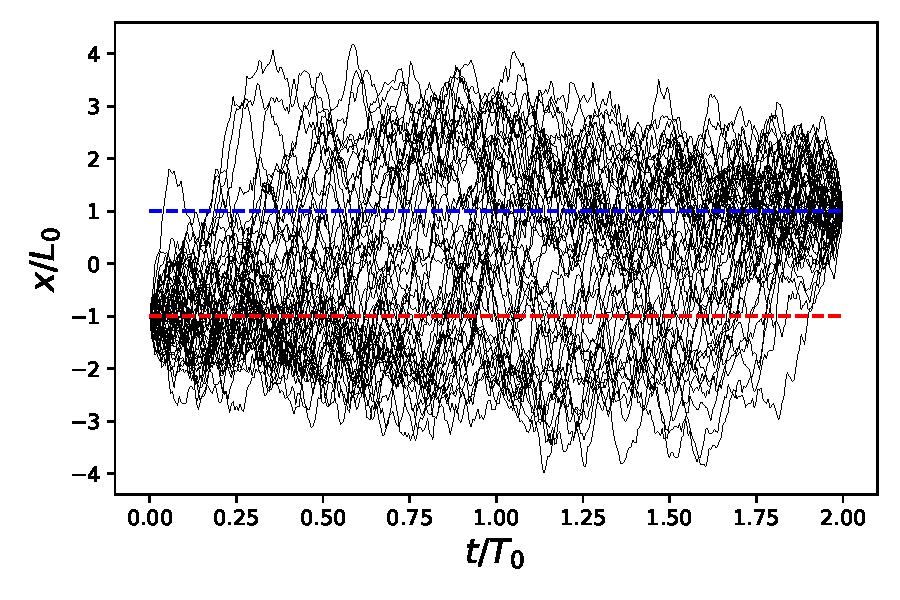
\includegraphics[width=\textwidth]{figs_part1/mcmc/1D_process_trajectories}
        \caption[]%
        {}    
        \label{fig:1D process trajectories hot}
    \end{subfigure}

	\vskip\baselineskip  

    \begin{subfigure}[b]{0.7\textwidth}
        \centering
        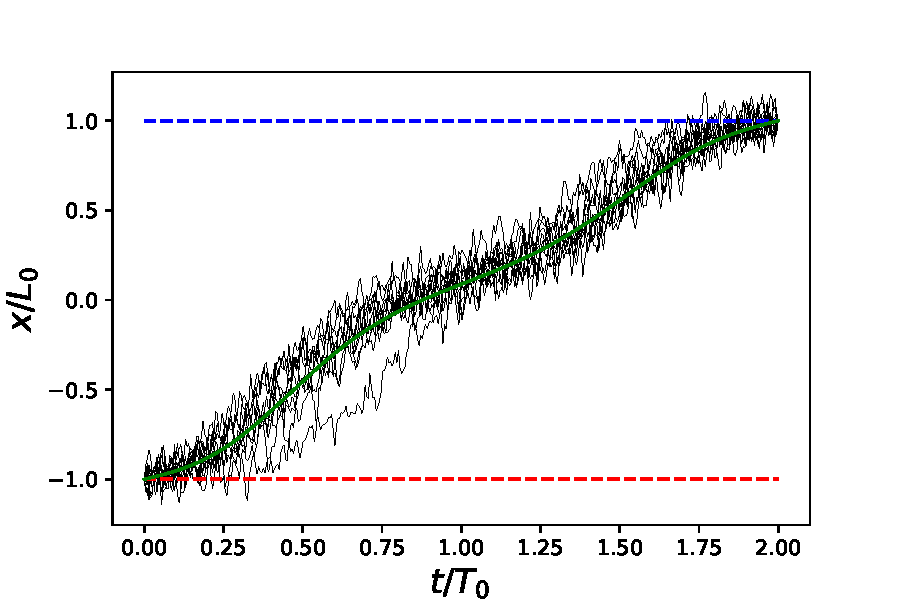
\includegraphics[width=\textwidth]{figs_part1/mcmc/1D_process_cold_trajectories}
        \caption[]%
        {}    
        \label{fig:1D process trajectories cold}
    \end{subfigure}     

    
    \caption[ ]
    {\small Simulation of the $1$-dimensional asymmetric double-well system (defined in Appendix \ref{app:The asymmetric double-well system}) using $M=10^8$ iterations of the pCN algorithm with burn-in $M_\text{B}/M = 0.3$. We sampled transition paths of duration $T/T_0 = 2$ between the minima at $x_0/L_0 = -1$ (red dashed lines) to the minima at $x_0/L_0 = 1$ (blue dashed lines), and with mode truncation $N = 200(T/T_0)$. (a) Shows $50$ transition paths at temperature $\theta / \theta_0 = 2$. (b) Shows $10$ transition paths at temperature $\theta / \theta_0$, and the instanton (green line).}
    \label{fig:1D process trajectories}
\end{figure*} 

Fig.~\ref{fig:1D process trajectories} shows the result of $M=10^8$ iterations of the pCN algorithm to a benchmark problem, with burn-in $M_\text{B}/M = 0.3$. We sample the TPE of a $1$-dimensional overdamped Langevin dynamics of a particle moving between the minima of an asymmetric double-well potential. See Appendix \ref{app:The asymmetric double-well system} for a figure of the potential and a detailed specification of the model. Fig.~\ref{fig:1D process trajectories hot} shows a sample of $50$ trajectories from the TPE, simulated at temperature $\theta/\theta_0 = 2$, where $\theta_0$ is a reference temperature. The reference temperature $\theta_0$ is defined such that at $\theta = \theta_0$ the thermal fluctuations equal the characteristic energy scale of the confining potential energy (See Appendix \ref{app:MCMC benchmark models} for details on the non-dimensionalisation of the model system). In Fig.~\ref{fig:1D process trajectories} Fig.~\ref{fig:1D process trajectories cold} we show the maximiser of the path-probability density functional Eq.~\ref{eq:path-probability meausure in terms of path-integral} (which we call the \textit{instanton}), as well as a sample of $10$ trajectories from the TPE simulated at a temperature $\theta/\theta_0 = 0.01$. The duration of the transition paths were $T /T_0 = 2$, where $T_0$ is a reference time-scale. We computed the instanton by minimising the Onsager-Machlup action of the model system, using a Ritz method as described in Ch.~\ref{ch:Ritz methods for Freidlin-Wentzel-Graham actions}. Note that, as mentioned in the introduction, at finite temperatures the instanton must be computed using Onsager-Machlup action, as opposed to the Freidlin-Wentzell action \citep{gladrowExperimentalMeasurementRelative2021a, adibStochasticActionsDiffusive2008a}. At temperatures $\theta > \theta_0$, where thermal fluctuations (represented by the noise term in the Langevin equation) dominate over the potential, and we see in Fig.~\ref{fig:1D process trajectories} (a) that the sample paths transition between the two minima several times. On the other hand, at temperatures $\theta \ll \theta_0$, where we would expect that transition events are rare, the TPE is concentrated around the instanton.


\begin{figure}[t]
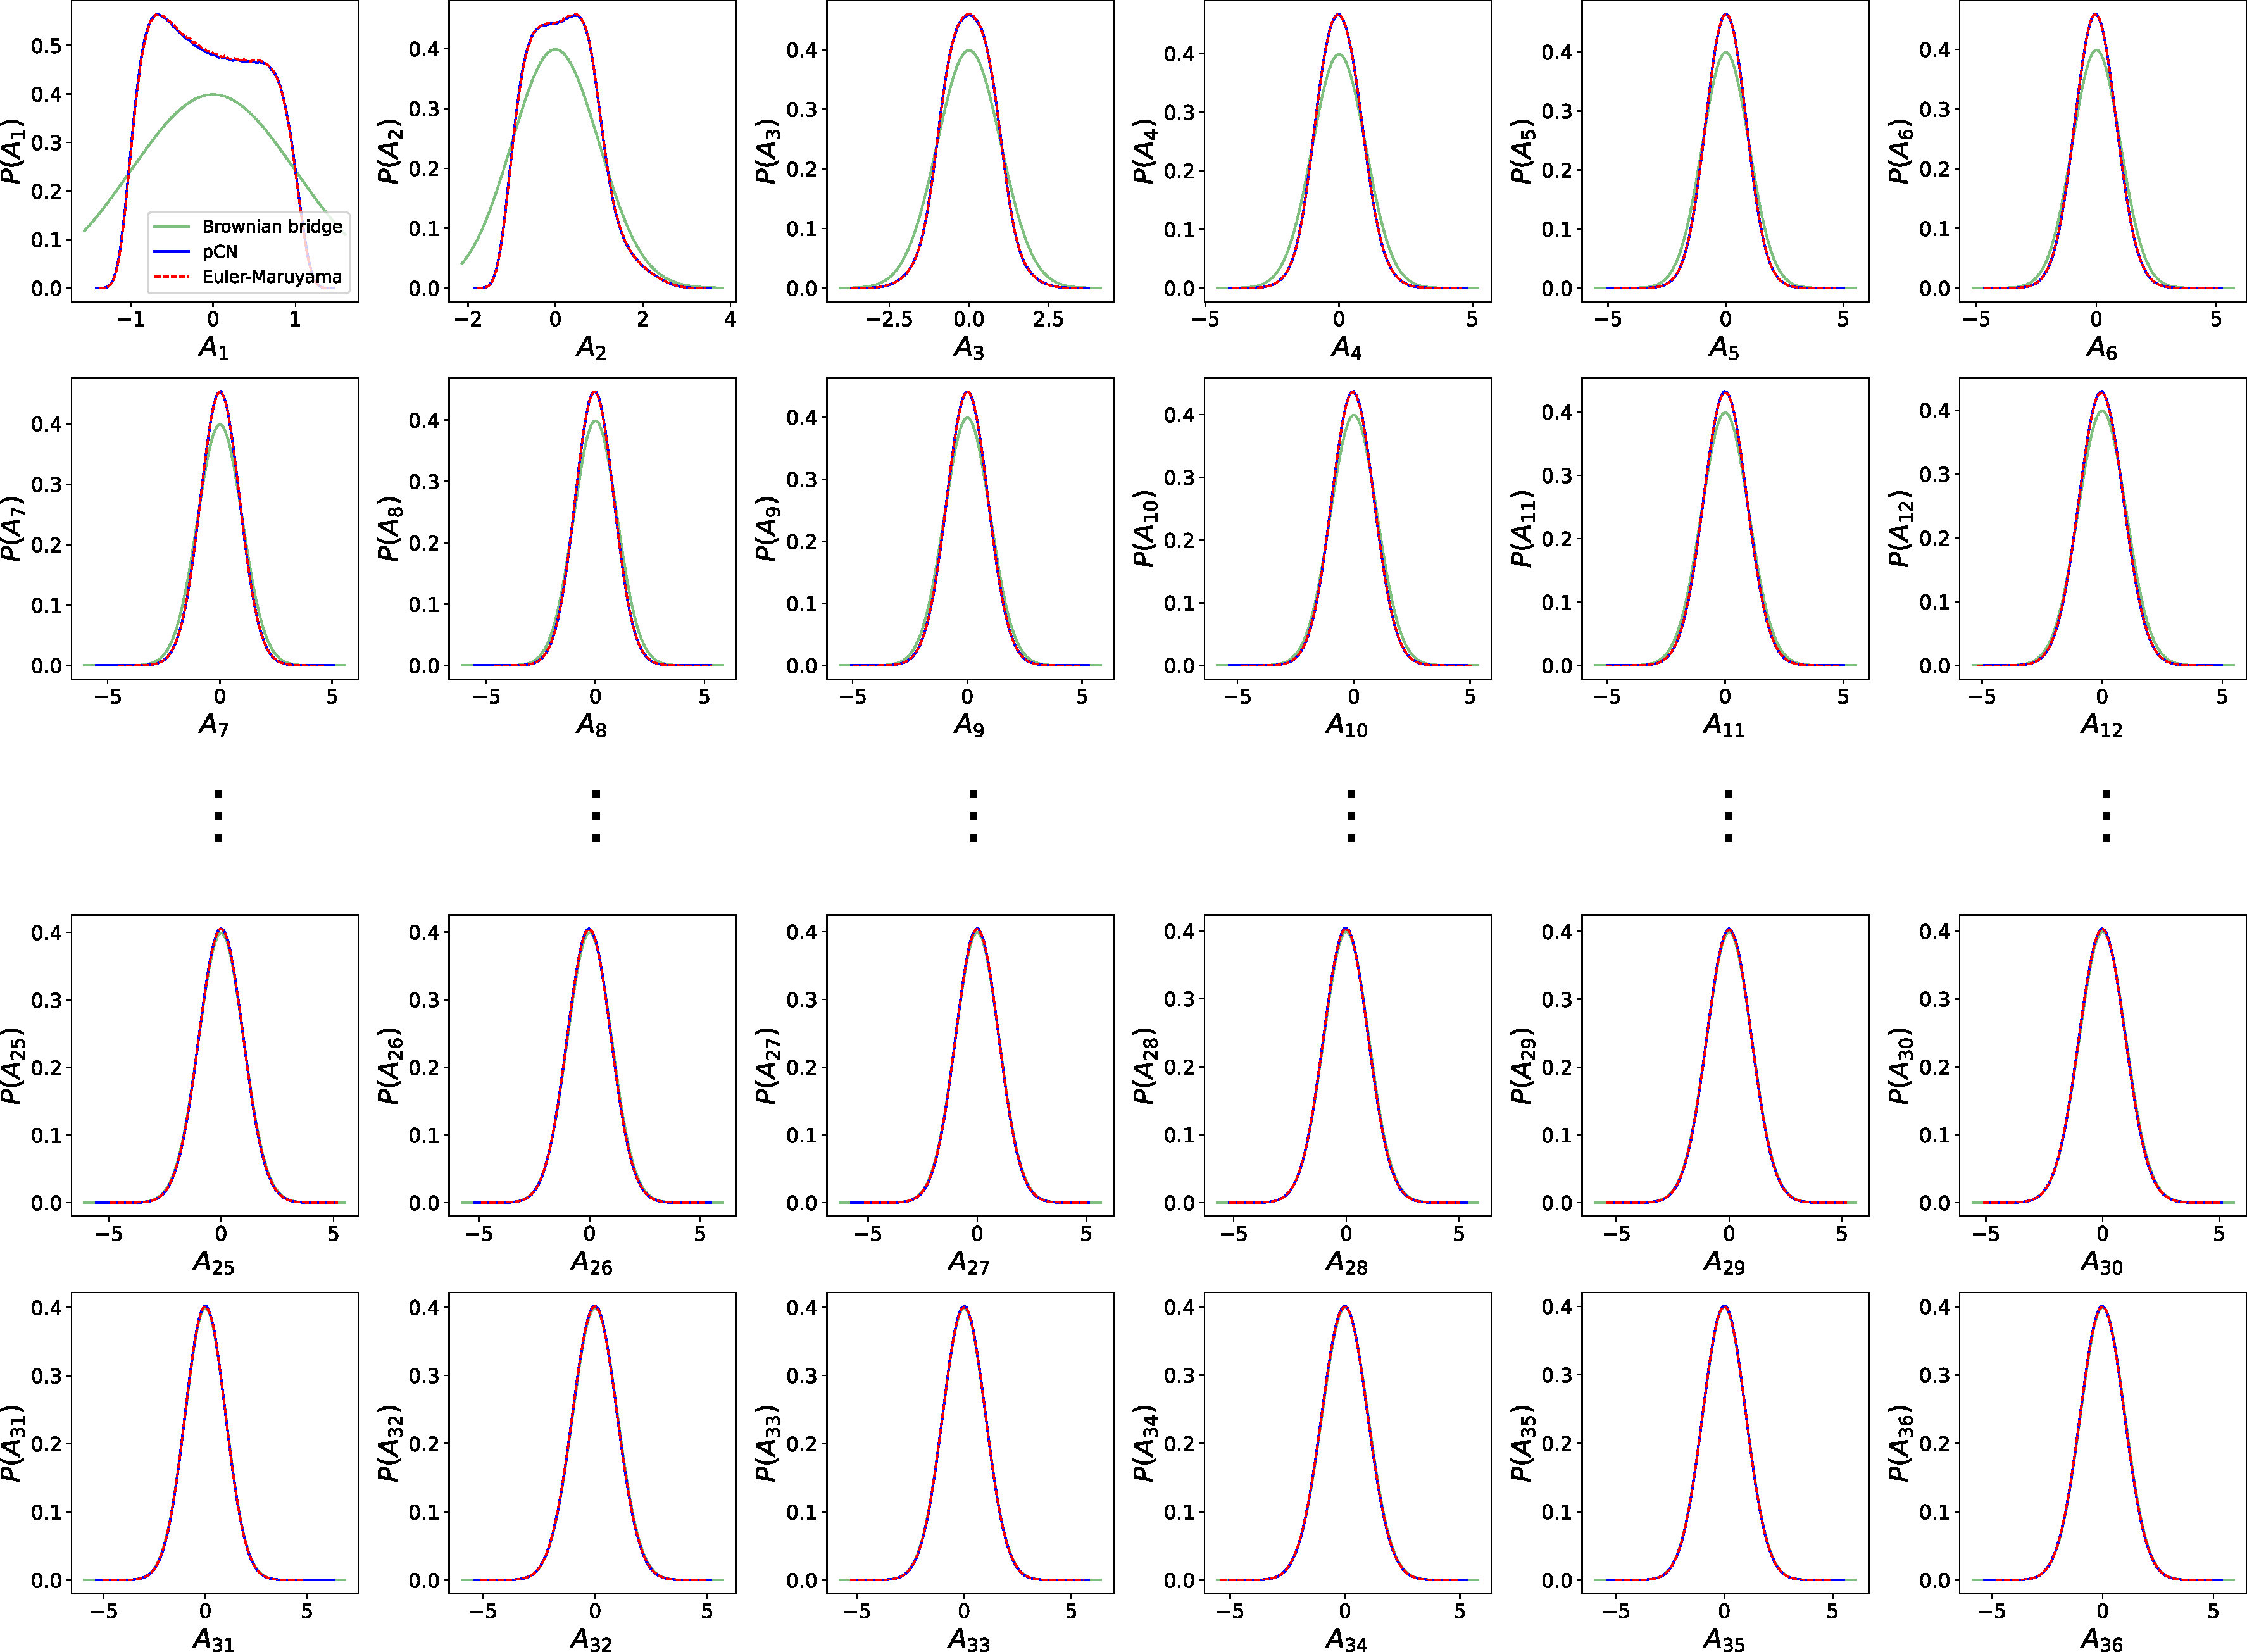
\includegraphics[width=0.98\textwidth]{figs_part1/mcmc/1D_process_MCMC_vs_Langevin}
\centering \caption{Simulation of the $1$-dimensional asymmetric double-well system using both the pCN and the Euler-Maruyama methods. The resulting samples of the latter were projected onto the KKL basis of the Brownian bridge process, and the figure shows the marginalised distribution over the coefficients $A_k$ of the sampled TPE. In each sub-plot, the green line are the distributions of a centred normal with unit-variance $Z_k \sim \mathcal{N}(0,1)$, which corresponds to the modes of the Brownian bridge process. The parameters of the simulation are the same as those of Fig.~\ref{fig:1D process trajectories} (a).}
\label{fig:1D process MCMC vs Euler-Maruyama} 
\end{figure}

To verify that our implementation of the algorithm correctly sampled the TPE, we verified our results using a standard Euler-Maruyama integrator \citep{kloedenNumericalSolutionStochastic2011}. Using the latter, we generated samples $10^6$ of the TPE by collecting trajectories
with end-points within a small interval $\tilde{x}(T)\in[1-\epsilon,1+\epsilon]$
around the right minima, where $\epsilon=10^{-2}$. We used a temperature $\theta / \theta_0$ as in Fig.~\ref{fig:1D process trajectories hot}, as it is unfeasible to use the Euler-Maruyama algorithm to sample the TPE for temperature regimes where transition events are rare. We projected the resulting sample paths onto the KKL basis of the Brownian bridge process, and compared the sample with the result of the pCN method. The results are showed in Fig.~\ref{fig:1D process MCMC vs Euler-Maruyama}, where we plot the marginalised histograms of the mode distributions against each other.

\subsection{Mode-space band structure} \label{sec:Mode-space band structure}

\begin{figure}[t]
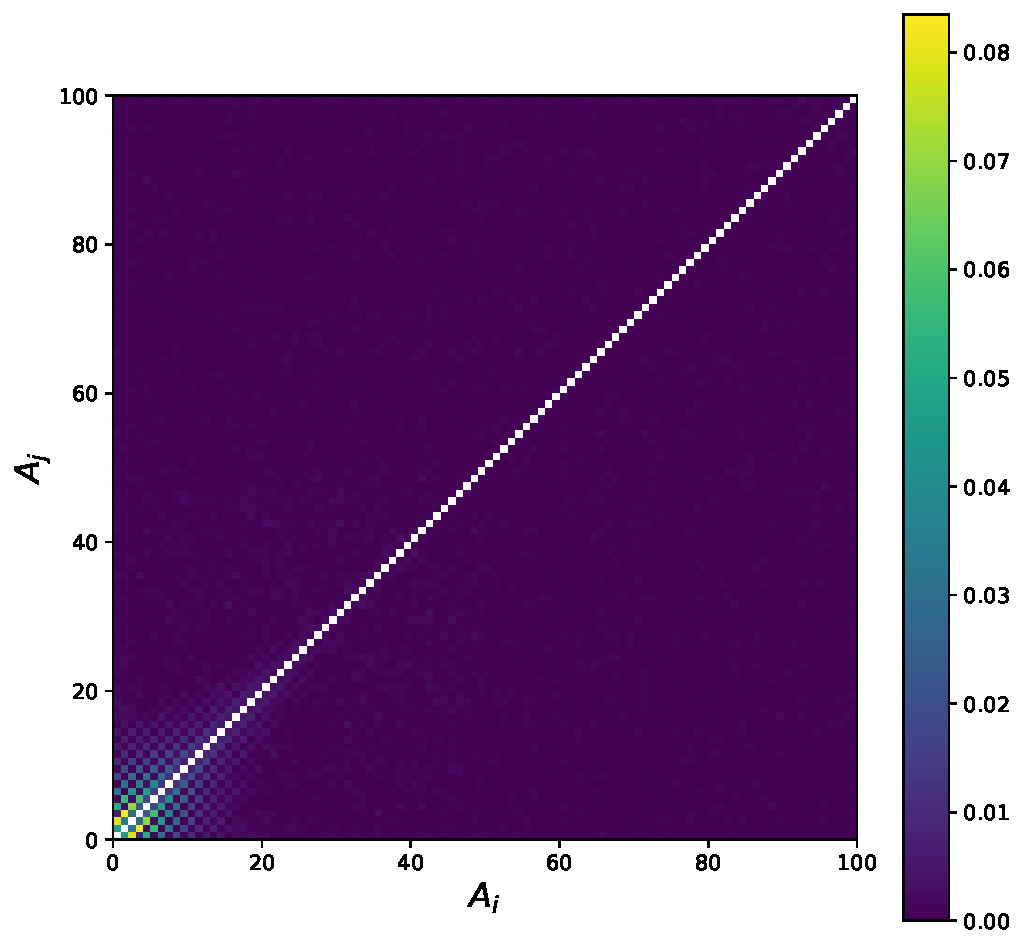
\includegraphics[width=0.7\textwidth]{figs_part1/mcmc/1D_process_covariances}
\centering \caption{The absolute normalised covariances $\rho_{kl} = \langle A_k A_l \rangle / \sqrt{ \langle A_k^2 \rangle \langle A_k^2 \rangle }$ of the first $100$ modes of the transition paths of the $1$-dimensional asymmetric double-well system. As $\rho_{kk} = 1,\ k=1,\dots,N$ by definition, we have excluded the diagonal from the plot. We sampled the TPE using the pCN algorithm, with parameters $T/T_0 = 2$, $\theta/\theta_0 = 2$ and $N = 200(T/T_0)$ with $M=10^8$ iterations. We see that there is a band separation between the low and high mode-numbers, where modes beyond the the $k \in [0, 40]$ quadrant are largely uncorrelated.}
\label{fig:1D process covariance} 
\end{figure}

In Fig.~\ref{fig:1D process MCMC vs Euler-Maruyama} we see that the marginalised distributions of the modes of stochastic trajectories in the TPE (blue lines) increasingly coincide with normal distributions of unit variance (green lines) at higher mode orders. The latter corresponds to the modes of the Brownian bridge process, as was established in Sec.~\ref{sec:Kosambi-Karhunen-Loeve expansions of stochastic trajectories}. Fig.~\ref{fig:1D process covariance} shows the absolute normalised covariances $\rho_{kl} = \langle A_k A_l \rangle / \sqrt{ \langle A_k^2 \rangle \langle A_k^2 \rangle }$ of the modes. Here we see the modes also rapidly decorrelate, and are numerically negligible beyond the first $30$ modes. Fig.~\ref{fig:1D process MCMC vs Euler-Maruyama} and Fig.~\ref{fig:1D process covariance} are a first indication that modes of transition paths are approximately distributed like a Brownian bridge process for large mode orders $k$. As we discuss and show below, this holds for \textit{any} It\^{o} diffusion with additive noise, regardless of the drift-field $\mathbf{b}$.

\begin{figure}[t]
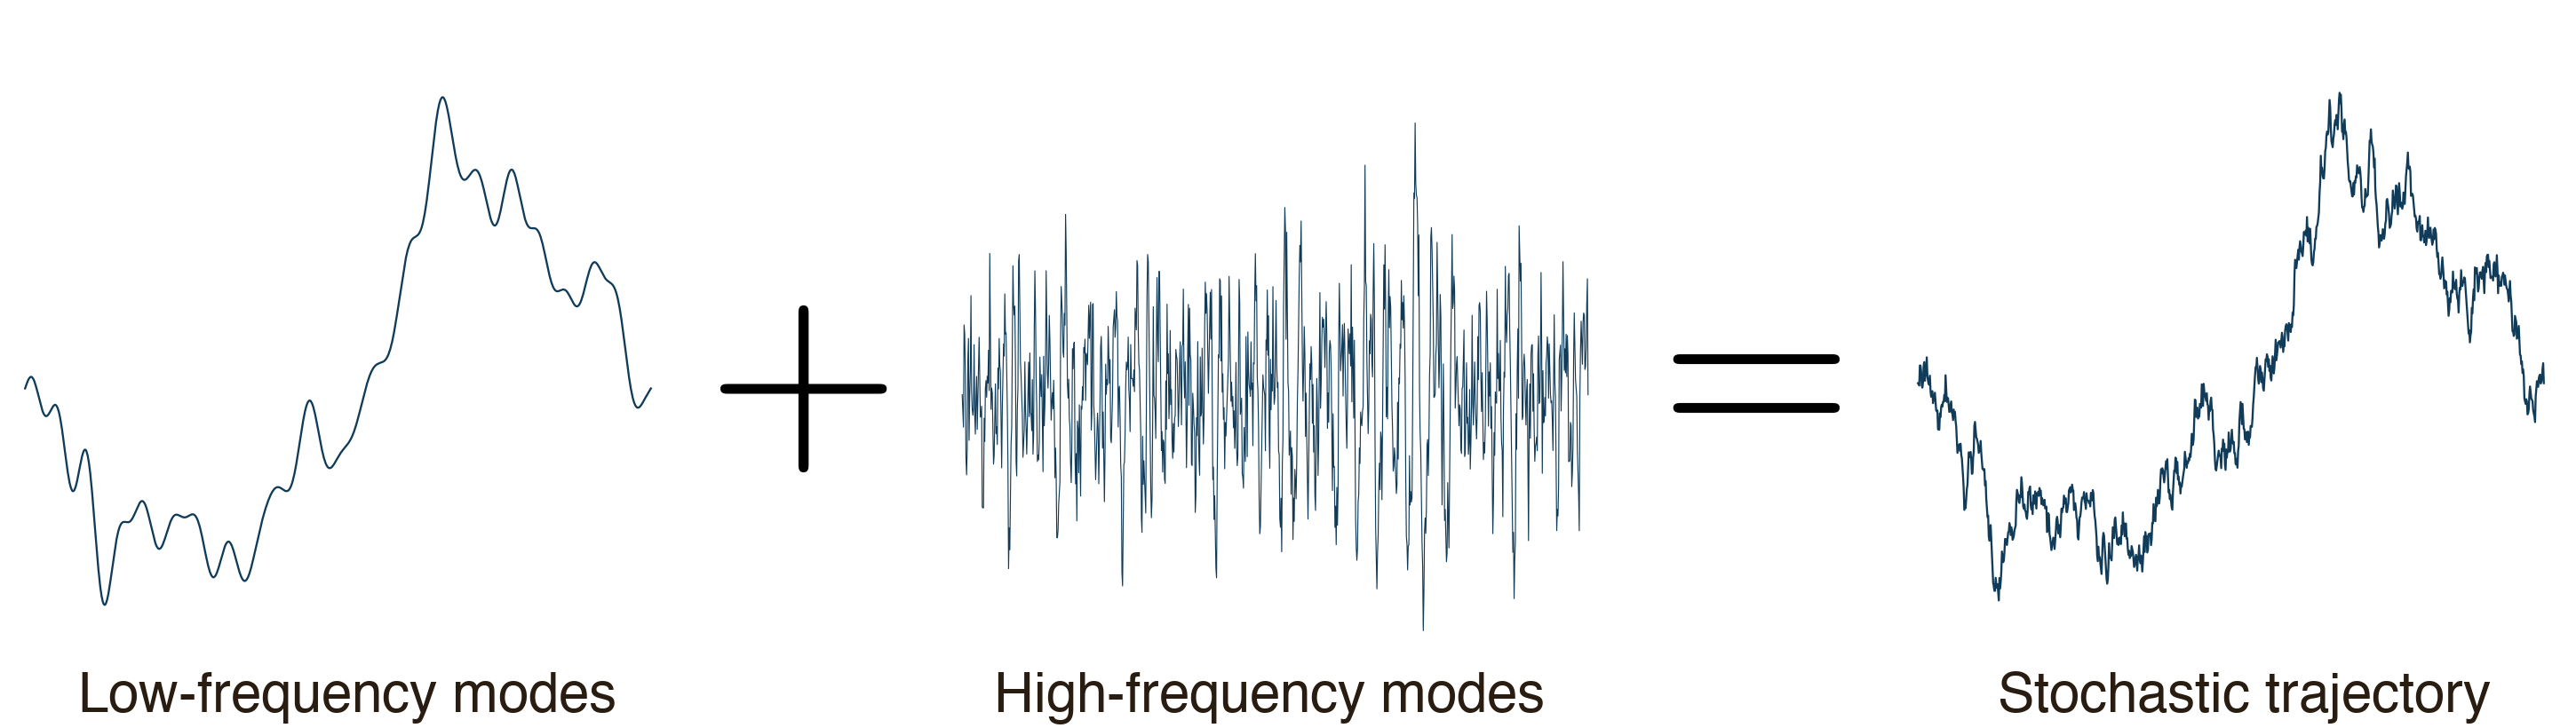
\includegraphics[width=0.95\textwidth]{figs_part1/mcmc/rough_path_decomposition}
\centering \caption{Illustration of the spectral decomposition of stochastic transition paths, in the Kosambi-Karhunen-Lo\`eve basis of the Brownian bridge process. Stochastic paths can be seen as the superposition of low-frequency modes, which resemble smooth trajectories, and zero-mean high-frequency noise. The general shape of the path is thus encapsulated in the former, whilst the latter adds roughness to the path. These same arguments can be made for a stochastic trajectory open end-point conditions, where the underlying Gaussian reference measure is then the Wiener process.}
\label{fig:rough path decomposition} 
\end{figure}

The law $\mathbb{P}_\mathbf{X}$ over the TPE of an It\^{o} diffusion can be seen as a non-linear transformation of $\mathbb{P}_\mathbf{B}$, the law of the Brownian bridge process. They are related via Eq.~\ref{eq:true path-space probability of TPE} in terms of the density Eq.~\ref{eq:radon-nikodym derivative of Px}, where the latter is an expression entirely in terms of the drift-field. Therefore, the difference in statistical `information' contained in $\mathbb{P}_\mathbf{X}$ relative to $\mathbb{P}_\mathbf{B}$ is exactly the drift-field $\mathbf{b}$. 

Furthermore, the difference in distribution between $\mathbb{P}_\mathbf{X}$ and $\mathbb{P}_\mathbf{B}$ is located in the lower-end of the mode-spectrum. For the $1$-dimensional benchmark problem, in Fig.~\ref{fig:1D process covariance} we can see a division in mode space between a low-frequency and high-frequency band, where the division between the two bands can be conservatively assigned to around $k_| = 40$. The low-frequency band thus correspond to the first $k_|$ modes in the expansion Eq.~\ref{eq:KKL expansion of transition paths}, and the high-frequency band correspond to all modes $k > k_|$. We can consider the low-frequency modes the `smooth' and the high-frequency modes the `rough' parts of a stochastic trajectory, as visualised in Fig.~\ref{fig:rough path decomposition}. The high-frequency noise is also centred, such that it does not effect the overall trajectory. The underlying shape of the path is thus only encoded in the low-frequency modes. In the dynamics of an It\^{o} diffusion Eq.~\ref{eq:ito diffusion equation}, the stochastic term $\sigma d\mathbf{W}$ dominates over deterministic drift-field $\mathbf{b}$ at short-time scales. In other words, $\mathbf{b}$ only affects the system on long time-scales. Therefore we would intuit that stochastic realisations $\mathbf{X}$, of the It\^{o} diffusion equation, look like they are undergoing drift-less free diffusion as we `zoom in' on the trajectory. Therefore, if $\mathbf{b}$ is smooth, we would expect that $\mathbb{P}_\mathbf{X}$ and $\mathbb{P}_\mathbf{B}$ only behave differently in the `smooth' low-frequency band, and behave identically in `rough' high-frequency band. Further numerical evidence of the band separation is provided indirectly in Sec.~\ref{sec:Mode-dependent step-sizes} and in later sections in Fig. \ref{fig:switch modes covariance} and Fig. \ref{fig:switch modes marginalised}, in addition to the results already discussed for the $1$-dimensional asymmetric double-well system above.

The band separation of the sampling method serves as an explanation for why the pCN method does not suffer from a curse of dimensionality as $N \to \infty$. As modes $k$ beyond some cutoff $k_|$ are approximately independently distributed normal random variables, the effective dimension of the target sampling space is $d k_|$, regardless of any choice of mode truncations $N > k_|$.

Statements analogous to the above would apply if we instead considered the spectrum of the law of an unpinned It\^{o} diffusion, with sample space $C_{\mathbf{x}_0}^0([0,T])$, the set of stochastic paths starting at $\mathbf{x}_0$ with open end-point conditions at $t=T$. In that case, using identical arguments, we would find that the spectrum of the $\mathbb{P}_\mathbf{X}$ would resemble $\mathbb{P}_\mathbf{W}$ in the high-frequency band, where the latter is the law of the Wiener process. Below we will provide an analytical argument for the case of an unpinned It\^{o} diffusion.

In the following we expand a unpinned Langevin processes of the form Eq. \ref{eq:ito diffusion equation} in the KKL basis of the Wiener process $\mathbf{W}$. For simplicity we only consider the $1$-dimensional case, but the results below readily generalises to higher dimensional processes. The KKL expansion of the $1$-dimensional Wiener process is
\begin{equation} \label{eq:wiener kkl expansion}
	W(t) = \mathbf{x}_0 +\sqrt{2 D} \sum_{k=1}^\infty Z_k \sqrt{\nu_k} \chi_k(t)
\end{equation}
where $Z_k,\ k =1,\dots,\infty$ are independent $d$-dimensional normal random variables distributed as $\mathbf{Z}_k \sim \mathcal{N}(0, \mathbbm{1}_d)$, and where
\begin{subequations}
	\begin{align}
		\chi_k(t) & = \sqrt{\frac{2}{T}} \sin (t / \sqrt{\nu_k}) \\
		\nu_k & = \frac{T^2}{\pi^2 \left(k - \frac{1}{2} \right)^2},
	\end{align}
\end{subequations}
and where $\chi_k(t)$ satisfy $\langle \chi_k, \chi_l \rangle = \delta_{kl}$, where we have defined
\begin{equation}
	\langle f, g \rangle = \int_0^T f(t) g(t) dt.
\end{equation}
for any two functions $f, g : [0,T] \to \mathbb{R}$. We begin with the integral form of the It\^{o} diffusion equation Eq.~\ref{eq:integral ito equation}
\begin{equation} \label{eq:integral ito equation 2}
X(t) = \int_0^t b(X(t')) dt' + \sqrt{2D} \int_0^{t} d W(t')
\end{equation}
where $b : \mathbb{R} \to \mathbb{R}$ is the drift-field, $t \in [0, T]$ and the second term of Eq.~\ref{eq:integral ito equation 2} is an It\^{o} integral. We assume, without loss of generality, that $X(0) = 0$. We now expand the Wiener process in its KKL expansion, and truncate the sum up to order $N$ to approximate Eq.~\ref{eq:integral ito equation 2} as
\begin{equation} \label{eq:Approximate ito integral solution}
X^N(t) = \int_0^t b(X^N(t')) dt' + \int_0^t dW^N(t')
\end{equation}
where $W^N$ is the truncation of Eq.~\ref{eq:wiener kkl expansion}, $X^N$ is the truncated stochastic process, and where the second term in Eq.~\ref{eq:Approximate ito integral solution} is now a Riemann-Stieltjes integral. It is a theorem (known as the \textit{Wong-Zakai theorem}) \citep{wongConvergenceOrdinaryIntegrals1965a, twardowskaWongZakaiApproximationsStochastic1996a, frizMultidimensionalStochasticProcesses2010a} that as $N\to\infty$ the sequence of solutions to Eq.~\ref{eq:Approximate ito integral solution} converges uniformly in probability to the solution of Eq.~\ref{eq:integral ito equation 2}\footnote{Note that the Wong-Zakai theorem holds for the Stratonovich formulation of Eq.~\ref{eq:integral ito equation 2}. However, for additive noise the It\^{o} and Stratonovich formulations are equivalent.}.


We we will expand $X^N$ as
\begin{equation}
	X^N(t) = \sqrt{2D} \sum_{k=1}^N A_k \sqrt{\nu_k} \chi_k(t).
\end{equation}
As $X^N(t)$ and $W^N(t)$ are smooth for finite $N$, we can take the derivative of Eq.~\ref{eq:Approximate ito integral solution} to find
\begin{equation} \label{eq:approximate ito equation}
	\dot{X}^N(t) = b(X^N(t)) + \dot{W}^N(t).
\end{equation}
We can expand the $\dot{X}^N(t)$ and $\dot{W}^N(t)$ as
\begin{subequations}
	\begin{align}
		\dot{X}^N(t) & = \sqrt{2 D} \sum_{k=1}^N A_k \psi_k(t) \\
		\dot{W}^N(t) & = \sqrt{2 D} \sum_{k=1}^N Z_k \psi_k(t)
	\end{align}
\end{subequations}
where
\begin{equation}
	\psi_k(t) = \sqrt{\nu_k} \dot{\chi}_k(t) = \sqrt{\frac{2}{T}} \cos(t / \sqrt{\nu_k}).
\end{equation}
As $\langle \psi_k, \psi_l \rangle = \delta_{kl}$, we have that $\psi_k$ forms an orthonormal basis over the space of paths. We can therefore expand the drift-field as
\begin{equation}
	b(X^N(t)) = \sqrt{2 D} \sum_{k=1}^N b_k \psi_k(t)
\end{equation}
where
\begin{equation} \label{eq:b_k}
	b_k = \frac{1}{\sqrt{2D}} \langle \psi_k, b(X^N) \rangle =  \int_0^T \psi_k(t) b(X^N(t)) dt.
\end{equation}
From Eq.~\ref{eq:approximate ito equation}, and the orthonormality of $\psi_k$, we get
\begin{equation} \label{eq:mode langevin}
	A_k = b_k + Z_k,
\end{equation}
where $k = 1,\dots, N$. This is a spectral version of the It\^{o} diffusion equation, where we have projected Eq.~\ref{eq:integral ito equation 2} onto the truncated KKL spectrum of the Wiener process. Here the mode coefficients $A_k$ are random variables expressed in terms of the drift modes $b_k$ and the modes of the Wiener process $Z_k$. From Eq.~\ref{eq:b_k} we see that $b_k = b_k(A)$ is in general a non-linear equation in terms of the mode coefficients $A = (A_1, \dots, A_N)$. We note that Eq.~\ref{eq:mode langevin} can in principle be used to sample the It\^{o} diffusion equation, by drawing $N$ random numbers $Z_k \sim \mathcal{N}(0,1)$ and then solving Eq.~\ref{eq:mode langevin} for $A$.

Any finite choice of the number of modes $N$ will lead to truncation errors, but for increasing $N$ Eq.~\ref{eq:mode langevin} will probabilistically convergence to the true infinite-dimensional distribution. For a given $X^N$, $b_k$ can be seen as the Fourier coefficients of $b$. Now, using the known convergence properties of Fourier expansions, we have that
\begin{equation}
	|b_k| \leq \frac{C(D, T)}{k}
\end{equation}
where $C(D, T)$ is some function of the system parameters. As $Z_k$ is always of order $1$, Eq.~\ref{eq:mode langevin} tells us that
\begin{equation}
	A_k \approx Z_k
\end{equation}
for $k > k_|$ for some value of $k_|$, and sufficiently large $N > k_|$. We thus see that for a given system, there are always only a finite number of physically relevant modes distinct from free diffusion dynamics. Therefore, the effective dimensionality of the target sample space is $dk_|$, for a general $d$-dimensional It\^{o} diffusion. In general $k_|$ be dependent on the drift-field $b$, and from Eq.\ref{eq:b_k} we see that it will be an increasing function of the duration $T$ and the diffusivity $D$. This latter fact is intuitive, as the influence of the drift-field in the dynamics increasingly dominates over the noise as the noise-amplitude $\sqrt{2 D}$ is lowered and $T$ is increased.

\subsection{Mode-dependent step-sizes} \label{sec:Mode-dependent step-sizes}

\begin{figure}[t]
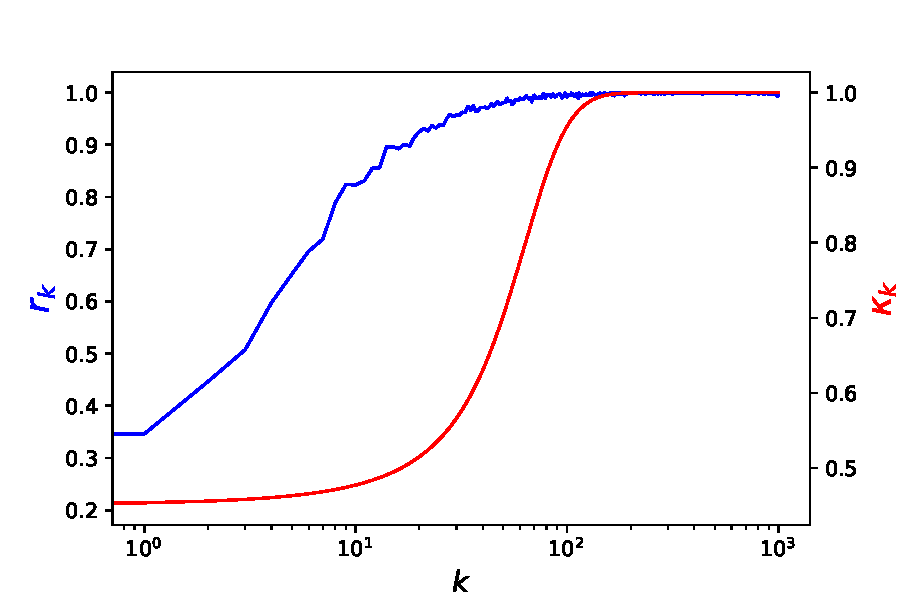
\includegraphics[width=0.9\textwidth]{figs_part1/mcmc/1D_process_acceptance_rate}
\centering \caption{ (Red line) The modal acceptance rates $r^\text{acc}_k$  for the $1$-dimensional asymmetric double-well system, with system parameters identical to those in Fig.~\ref{fig:1D process trajectories hot}. (Blue line) A sigmoidal step-size profile $\kappa_k$.}
\label{fig:1D process acceptance rate} 
\end{figure}

The band-structure of the mode-spectrum of It\^{o} processes can potentially be exploited to improve the sampling algorithm. Here, as a simple first attempt, we will use the band-structure to adapt the step-sizes in the pCN algorithm for each individual mode. To construct an adapted step-size matrix $\kappa_{ik}$, we need to first have a method by which to estimate the extent to which each mode is distributed like a Gaussian. Note that if $\kappa_{ik} = 1$ for a given $i,k$, then the proposal Eq.~\ref{eq:pCN proposal numerical algo} at each iteration is an independent random sample from $\mathcal{N}(0,1)$.

Consider a modified pCN algorithm that, at each iteration step $n$, only updates a single mode $A_{ik}$ at a time. The algorithm updates the mode in sequence, such that after $d N$ iterations all of the modes $A_{ik},\ i=1,\dots,d,\ k=1,\dots,N$ will have been updated once. Let $r_{ik}$ be the \textit{modal acceptance rate} of the iterations of the mode $A_{ik}$, which is the ratio of accepted proposals to the number of iterations $M/(dN)$, where $M$ is the number of iterations of the whole algorithm. Similarly, let $r$ be the acceptance rate of all modes in the regular pCN algorithm. Figure ~\ref{fig:1D process acceptance rate} plots the modal acceptance rates (blue line) for the $1$-dimensional asymmetric double-well system, with system parameters identical to those in Fig.~\ref{fig:1D process trajectories hot}, mode truncation $N = 1000$ and iterations $M = 1000N$. We see that $r_k \approx 1$ for modes $k \geq 50$. Therefore we may consider a sigmoidal step-size profile
\begin{equation} \label{eq:kappa profile}
	\kappa_k = \kappa_\text{min} + \frac{\kappa_\text{max} - \kappa_\text{min}}{1 + \exp\left( - \sigma_\kappa ( k - k_|) \right)}
\end{equation}
with $\kappa_\text{min} = 0.4$, $\kappa_\text{max}=1$, $k_| = 50$ and $\sigma_\kappa = 0.05$, which is plotted in Fig.~\ref{fig:1D process acceptance rate} (blue line). The base-line step-size $\kappa_\text{min}$ was computed by finding an approximate constant $\kappa_{k} = \bar{\kappa}$ that yielded an acceptance rate $r \approx 0.3$ in the regular pCN algorithm.

\begin{figure}[t]
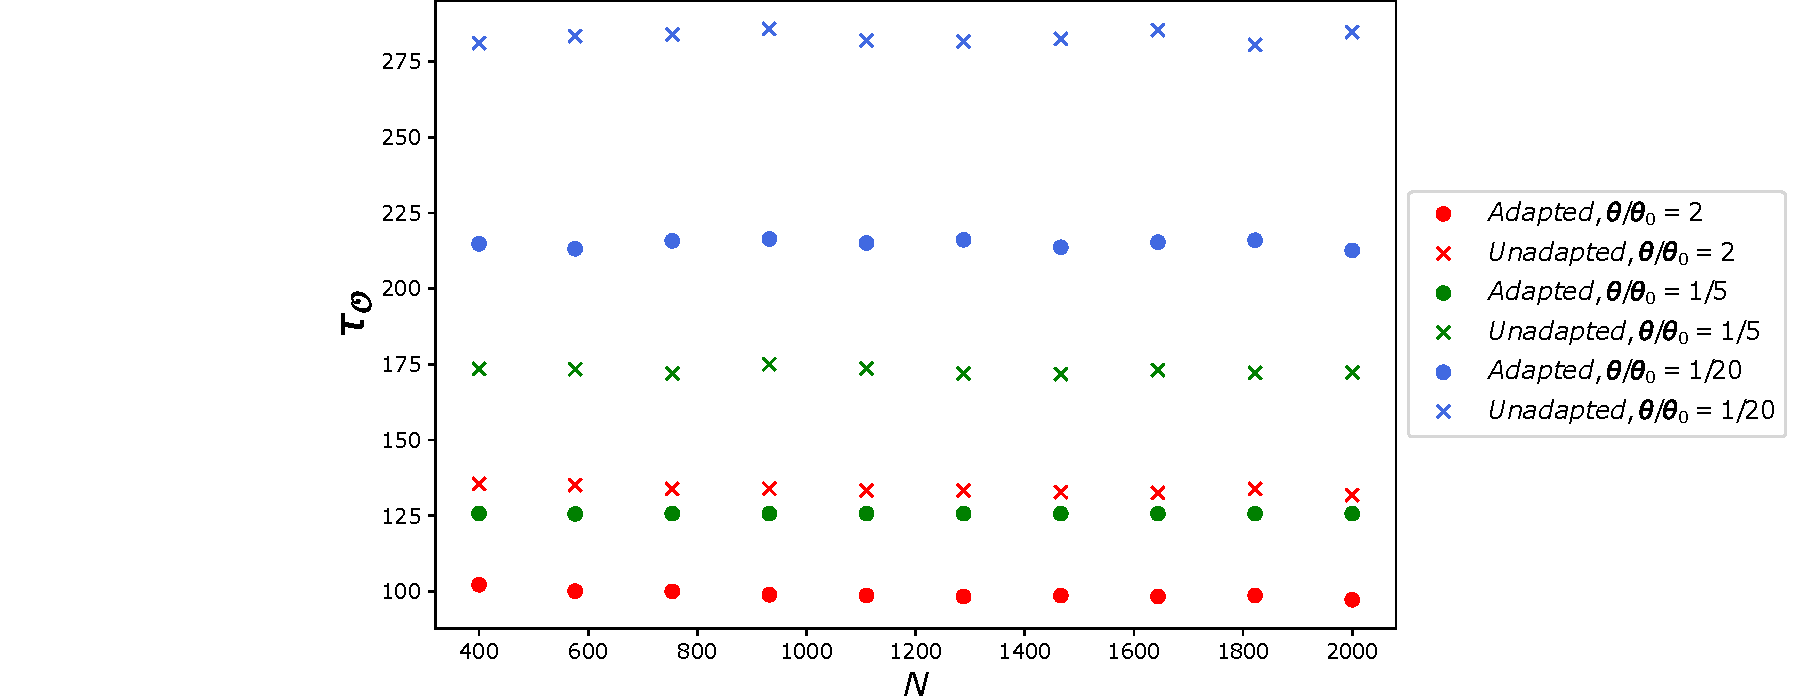
\includegraphics[width=0.98\textwidth]{figs_part1/mcmc/autocorrelation_benchmarks}
\centering \caption{ The auto-correlation times $\tau_{\mathcal{O}}$ of MCMC runs of the asymmetric double-well system at temperatures $\theta/\theta_0 = 2, 1/5,1/20$ with adapted and unadapted modal step-sizes $\kappa_i$, for varying mode truncations $N$.}
\label{fig:1D autocorrelation benchmarks} 
\end{figure}

We benchmarked MCMC runs with adapted step-size profiles against runs with constant steps-sizes by considering their relative \textit{auto-correlation times}. Let $\mathcal{O}[\mathbf{X}]$ be some observable, and $X^{(n)},\ n=1,\dots,M$ the result of an MCMC run. Then the expectation $\langle \mathcal{O}[\mathbf{X}] \rangle$ can be estimated using Eq.~\ref{eq:MCMC expectation}, and the variance as
\begin{equation} 
	\text{Var}(\mathcal{O}[\mathbf{X}]) = \langle (\mathcal{O}[\mathbf{X}] - \langle \mathcal{O}[\mathbf{X}] \rangle)^2 \rangle = \frac{\tau_\mathcal{O}}{M} \sum_{n=1}^M (\mathcal{O}[\mathbf{X}^{(n)}] - \langle \mathcal{O}[\mathbf{X}] \rangle)^2,
\end{equation}
where $\tau_\mathcal{O}$ is the \textit{integrated autocorrelation time} for the chain $\mathcal{O}[\mathbf{X}^{(n)}],\ n=1,\dots,M$. It carries the interpretation of the amount of iterations required for the MCMC to `forget' where it began, such that the effective number of samples is $M/\tau_\mathcal{O}$. See \citep{sokalMonteCarloMethods1997, goodmanEnsembleSamplersAffine2010} for detailed definitions and how to estimate $\tau_\mathcal{O}$. In Fig.~\ref{fig:1D autocorrelation benchmarks} we show the results of the benchmark runs. For mode truncations varying between $N=400$ and $N=2000$, we computed the auto-correlation times for MCMC runs with an adapted step-size $\kappa_k$ as in Eq.~\ref{eq:kappa profile}, as well as an unadapted step-size $\kappa_k = \kappa_\text{min}$. We ran simulations at temperatures $\theta/\theta_0 = 2, 1/5,1/20$, with $\kappa_\text{min} = 0.4, 0.35, 0.3$ respectively, and $\kappa_\text{max}=1$, $k_| = 50$ and $\sigma_\kappa = 0.05$ for all temperatures. We see that the adapted step-size runs enjoy lower autocorrelation times.

The above is a modest attempt at utilising the band-structure to improve autocorrelation times. A more promising avenue would be to apply a multi-level MCMC algorithm \citep{gilesMultilevelMonteCarlo2008, dodwellHierarchicalMultilevelMarkov2015, jansenMultilevelMonteCarlo2020, rohrbachMultilevelSimulationHardsphere2022}, which consists of a series of $M_\text{multi}$ chains with a hierarchy of mode truncations $N_{i},i=1,\dots,M_\text{multi}$ such that $N_{i} < N_{i+1}$. The MCMC can be efficently run on the lowest-dimensional chain, and then be \textit{upsampled} via the multi-level scheme, such that we generate samples of the highest $N_{M_\text{multi}}$-dimensional system.





\subsection{Generalised end-point conditions} \label{sec:Generalised end-point conditions}

So far we have considered transition path ensembles with fixed end-point conditions. We may consider a TPE of a more a general form
\begin{equation}
	E_{R_0}^{R_T}([0,T]) = \{ \mathbf{X}\ :\ \mathbf{X} \in C_{\mathbf{x}_0}([0,T]) \text{ and } \mathbf{X}(T) = \mathbf{x}_T \text{ where } \mathbf{x}_0 \in R_0,\ \mathbf{x}_T \in R_T \}.
\end{equation}
In other words, $E_{R_0}^{R_T}([0,T])$ is the set of stochastic paths that start in $R_0 \subset \mathbb{R}^d$ and end in $R_T \subset \mathbb{R}^d$. In applications, $R_0$ and $R_T$ may, for example, be chosen to lie within the basins of attraction of fixed points of the drift-field $\mathbf{b}$.

A probability measure over $E_{R_0}^{R_T}([0,T])$ can be constructed by simply grafting a probability distribution over the initial condition onto the path-probability measure $\mathbb{P}_\mathbf{X}$. Let $\pi_0$ be a probability measure over $R_0$, with density $p_0 \sim \pi_0$. Let $\tilde{P}_\mathbf{X}$ be a probability measure over $E_{R_0}^{R_T}([0,T])$, defined in terms of the density $\tilde{P}_\mathbf{X} \sim \tilde{\mathbb{P}}$
\begin{equation}
	\tilde{P}_\mathbf{X}[\mathbf{x}] \propto p_0(\mathbf{x}(0)) P_\mathbf{X}[\mathbf{x}]
\end{equation}
where we have restricted the domain of $\tilde{P}_\mathbf{X}[\mathbf{x}]$ to paths that satisfy $\mathbf{x}(0) \in R_0$ and $\mathbf{x}(T) \in R_T$.

We can modify the pCN algorithm to sample $\tilde{P}_\mathbf{X}$. In addition to the coefficient matrix $A = ( \mathbf{a}_1\ \mathbf{a}_2 \dots \mathbf{a}_N )$, the MCMC state will now also be specified by the starting- and end-points of the transition path $\mathbf{x}_0$ and $\mathbf{x}_T$ respectively. We define the new update rule
\begin{subequations} \label{eq:open endpoints pCN}
	\begin{align}
		\mathbf{a}'_i & = \sqrt{1 - \kappa^2} \mathbf{a}^{(n)} + \kappa \mathbf{Z}_i \\
		& \text{Draw } \mathbf{x}'_0 \text{ from } \pi_0 \label{eq:open endpoints pCN x0} \\
		& \text{Draw } \mathbf{x}'_T \text{ from } \pi_T \label{eq:open endpoints pCN xT}
	\end{align}
\end{subequations}
where $\pi_T$ is a distribution over $R_T$ that must be specified. Let $p_T \sim \pi_T$, then the transition kernel density is
\begin{equation}
	\tilde{Q}[\mathbf{X} \to \mathbf{Y}] = p_0(\mathbf{Y}(0)) p_T(\mathbf{Y}(T)) Q_\text{pCN}[\mathbf{X} \to \mathbf{Y}].
\end{equation}
From Eq.~\ref{eq:MCMC acceptance probability (non rigorous)} we find the acceptance probability
\begin{equation}
	\tilde{A}[\mathbf{X}, \mathbf{Y}] = \text{min} \left\{
		1,
		e^{\Phi[\mathbf{X}] - \Phi[\mathbf{Y}]} \frac{p_T(\mathbf{X}(T))}{p_T(\mathbf{Y}(T))}
	\right\},
\end{equation}
where transition paths are expanded as
\begin{equation} \label{eq:KKL expansion of transition paths 2}
	\mathbf{X}^N(t;A,\mathbf{x}_0, \mathbf{x}_T) = \mathbf{x}_0 + (\mathbf{x}_T - \mathbf{x}_0) \frac{t}{T} +\sqrt{2 D} \sum_{i=1}^N \mathbf{a}_i \sqrt{\lambda_i} \phi_i(t).
\end{equation}


The update rule Eq.~\ref{eq:open endpoints pCN} has not been numerically tested, but is rather offered here as a proof-of-concept to show that it is possible to implement generalised initial- and final end-point configurations using the pCN method. Equation ~\ref{eq:open endpoints pCN x0} and Eq.~\ref{eq:open endpoints pCN xT} are here independent samplers, and in practice implementing random-walk procedures in $R_0$ and $R_T$ might lead to better convergence.

Finally, some applications may require that we let $r$ of the $d$ degrees of freedom have open end-point conditions (In other words, $R_T = \mathbb{R}^d$). Let $X_i$ be the components of the stochastic process $\mathbf{X}$, and we consider transition paths where we let $X_i,\ i=1,\dots,r$ have open end-point configurations. We may then adapt the pCN algorithm of Sec.~\ref{sec:pCN Numerical algorithm summary} by expanding $X_j,\ j=r+1,\dots,d$ in the KKL basis of the Brownian bridge process as before, and expanding $X_i,\ i=1,\dots,r$ in the KKL basis of the \textit{Wiener process}.

% In applications we could, for example, let the initial configuration-space extend to all of state-space $R_0 = \mathbb{R}^d$, and let $\pi_0$ be the steady-state distribution of the It\^{o} diffusion. That is, $\pi_0$ is the distribution $\mathbf{X}(T)$ as $T \to \infty$ (this distribution is independent of the initial state $\mathbf{X}(0)$). For most It\^{o} diffusions the steady state distribution is not known analytically, however it can be approximated by simulating 


\section{Sampling multi-modal transition path ensembles} \label{sec:Teleporter MCMC}

Many applications of MCMC methods involve state-spaces that consist of large or very complicated probability landscapes. In particular, the target probability measure may be concentrated around several local maxima that are far-removed from each other in state-space. In such cases, one of the major difficulties that MCMC methods face is either the slow or complete failure of the chain to mix between the local maxima of the target measure. Inherently, the issue stems from the fact that the samples generated by the MCMC are not independent, but correlated. That is, a future state $X^{(n+1)}$ will often lie within the general vicinity of the current state $X^{(n)}$ in the chain. If $X^{(n)}$ is in a region of locally high probability in state-space, then the likelihood of the chain to traverse to another local maximum is low if the two regions are separated by regions of low probability. In this section, we will develop an algorithm which allows for simultaneously sampling multiple local maxima. We will begin by first defining the algorithm for finite dimensional spaces, and then in subsequent subsections we will develop the necessary theory to define the method on the transition path ensembles of It\^{o} diffusions.

\begin{figure*} 
    \centering
    \begin{subfigure}[b]{0.47\textwidth}  
        \centering 
        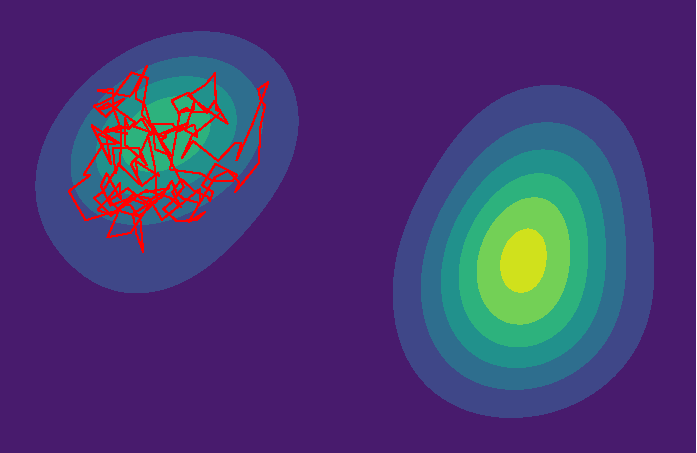
\includegraphics[width=\textwidth]{figs_part1/mcmc/example_2D_dist_with_RMW}
        \caption[]%
        {}    
        \label{fig:example_2D_dist_with_RMW}
    \end{subfigure}
    \hfill
    \begin{subfigure}[b]{0.47\textwidth}
        \centering
        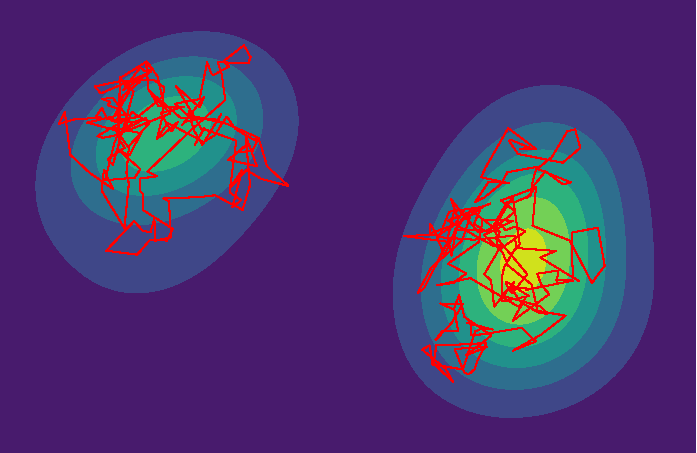
\includegraphics[width=\textwidth]{figs_part1/mcmc/example_2D_dist_with_TMC}
        \caption[]%
        {}    
        \label{fig:example_2D_dist_with_TMC}
    \end{subfigure}
    \caption[ ]
    {\small MCMC samples of a $2$-dimensional distribution with two segregated regions of high probability. (a) An illustration of an RMW scheme that fails to mix between the two regions. (b) An illustration of the TMC scheme, that teleports between the two regions to sample both simultaneously. }
\end{figure*} 

%consisting of a weighted mixture of two multi-variate Gaussians. If the means of the two Gaussians are sufficiently displaced from each other, and if their variances are such that they have negligible overlap, then we expect slow mixing to be likely during sampling. Fig.~\ref{fig:example_2D_dist_with_RMW} illustrates an example of an RMW sampling a mixture of two $2$-dimensional multi-variate Gaussians. Whilst the chain will thoroughly sample the local vicinity of its current state, it might only rarely traverse between the Gaussians. The resulting sample might not be representative of the target measure, as it is incorrectly skewed towards one of the two Gaussians. 

As a motivating example, consider a target measure with a $2$-dimensional state space with two local maxima. If the support of the measure is heavily concentrated around the two maxima, and if the two regions are sufficiently segregated from each other, then we expect slow mixing to be likely during sampling. Fig.~\ref{fig:example_2D_dist_with_RMW} illustrates an example of an RMW sampling such a distribution. Whilst the chain will thoroughly sample the locally connected region, it might only rarely traverse between the two regions. The resulting sample will not be representative of the target measure, as it is incorrectly skewed towards one maximum at the expense of the other.

The issue of slow mixing can be mitigated via a simple modification of the MCMC proposal rule. Consider a general target measure $\mathbb{P}$ with density $P \sim \mathbb{P}$ over $\mathbb{R}^d$, and an MCMC scheme defined by the transition kernel $T(\mathbf{x} \to \mathbf{y})$, which has $\mathbb{P}$ as its invariant measure. Furthermore, let $p_\text{T} \in [0,1]$ and let $T_\text{T}(\mathbf{x} \to \mathbf{y})$ be an additional MCMC scheme with the same target measure we will define below. We define the superposition of the two schemes as
\begin{equation} \label{eq:TMC transition kernel}
	T_\text{TMC} (\mathbf{x} \to \mathbf{y}) = (1 - p_\text{teleport}) T(\mathbf{x} \to \mathbf{y}) + p_\text{T} T_\text{T}(\mathbf{x} \to \mathbf{y}).
\end{equation}
Equation \ref{eq:TMC transition kernel} defines a Markov chain with $\mathbb{P}$ as its invariant measure, that, with probability $p_\text{teleport}$ transitions using $T_\text{T}(\mathbf{x} \to \mathbf{y})$, and with probability $1-p_\text{teleport}$ transitions using $T(\mathbf{x} \to \mathbf{y})$. The key idea behind the algorithm is to fashion $T_\text{T}(\mathbf{x} \to \mathbf{y})$ such that the MCMC can `teleport' between segregated local regions of high probability, will therefore call $T_\text{T}(\mathbf{x} \to \mathbf{y})$ the \textit{teleportation kernel}. Let $\mathbb{P}_\text{T}$ be a probability measure we call the \textit{teleportation measure}, with density $P_\text{T} \sim \mathbb{P}_\text{T}$, that we can efficiently draw independent samples from. We now construct $T_\text{T}(\mathbf{x} \to \mathbf{y})$ using the Metropolis-Hastings scheme Eq.~\ref{eq:Metropolis-Hastings transition kernel}, with proposal kernel
\begin{equation} \label{eq:teleportation proposal}
	Q_\text{T}(\mathbf{x} \to \mathbf{y}) = P_\text{T}(\mathbf{y}),
\end{equation}
and from Eq.~\ref{eq:MCMC acceptance probability (non rigorous)} we find the acceptance kernel
\begin{equation} \label{eq:teleportation acceptance}
	A_\text{T}(\mathbf{x}, \mathbf{y}) = \text{min} \left\{
		1, \frac{P[\mathbf{y}] P_\text{T}(\mathbf{x}) }{P[\mathbf{x}] P_\text{T}(\mathbf{y}) }.
	\right\}
\end{equation}
The second term of Eq.~\ref{eq:TMC transition kernel} thus draws proposal states independently from $\mathbb{P}_\text{T}$. Now if $\mathbb{P}_\text{T}$ is some suitable choice of teleportation measure that concentrates around the local maxima of the target measure $\mathbb{P}$, the resulting MCMC scheme Eq.~\ref{eq:TMC transition kernel} will be able to `teleport' between maxima with some probability at each iteration. We call this the \textit{teleporter MCMC} scheme (TMC). Similar algorithms have been proposed in \citep{sminchisescuModeHoppingMCMCSamplera, lindseyEnsembleMarkovChain2021}. Fig.~\ref{fig:example_2D_dist_with_TMC} shows an illustrative example of a TMC run.

Note that the TMC requires knowledge of the extrema of the distribution. However, as numerical optimisation is in general computationally cheaper than MCMC sampling, finding the maxima of the target measure is often feasible. In the case of paths-spaces, Ritz methods of the kind described in Ch.~\ref{ch:Ritz methods for Freidlin-Wentzel-Graham actions} can be used. Once the maxima have been found, there are in principle many choices for $\mathbb{P}_\text{T}$. However, from Eq.~\ref{eq:teleportation acceptance} we see that care must be taken so that the teleportation measure does not generate proposals that are probabilistically unfavourable.

One way to ensure the suitability of the teleportation measure is by constructing it as a superposition of multi-variate Gaussians, that each locally approximates $\mathbb{P}$ around each maximum. Let $V(\mathbf{x}) = \log P(\mathbf{x})$ be the exponential scaling of the target measure density, and let $\mathbf{x}^[\alpha],\ \alpha=1,\dots,K$ be the $K$ local maxima of $P(\mathbf{x})$. Then we can approximate $P(\mathbf{x})$ around $\mathbf{x}^{[\alpha]}$ by Taylor expanding $V(\mathbf{x})$ to second order. We get
\begin{equation} \label{eq:local expansion of P}
	P_G^{[\alpha]}[\mathbf{x}] = \frac{1}{\mathcal{Z}^{[\alpha]}} \exp \left( - \frac{1}{2}  ( \mathbf{x} - \mathbf{x}^{[\alpha]} )^T H^{[\alpha]} ( \mathbf{x} - \mathbf{x}^{[\alpha]} ) \right)
\end{equation}
where $\mathcal{Z}^{[\alpha]}$ is a normalisation constant and
\begin{equation}
	H^{[\alpha]}_{ij} = (\partial_i \partial_j V) |_{\mathbf{x} = \mathbf{x}^{[\alpha]} }.
\end{equation}
The Hessian matrix $H^{[\alpha]}$ is, in this context, known as the \textit{precision matrix} of the multi-variate Gaussian $\mathbb{P}_G^{[\alpha]}$. Correspondingly, we have that $(H^{[\alpha]})^{-1}$ is the covariance matrix, such that we can write $\mathbb{P}_G^{[\alpha]} \sim \mathcal{N}(\mathbf{x}^{[\alpha]}, (H^{[\alpha]})^{-1})$. Using Eq.~\ref{eq:local expansion of P} we construct the teleportation measure as
\begin{equation} \label{eq:teleportation measures mixed gaussian}
	P_\text{T}(\mathbf{x}) = \sum_\alpha^{K} w_\alpha P_G^{[\alpha]}(\mathbf{x})
\end{equation}
where $w_\alpha$ are tuneable weights that must satisfy $\sum_{\alpha=1}^{K}w_{\alpha}=1$.

In the following subsections, we will be generalising the TMC to infinite-dimensional path-spaces. In this setting, our aim is to effectively sample the TPEs of systems that have multiple competing transition channels. At low diffusivity (low temperature), these channels concentrate around the \textit{local instantons} $\mathbf{x}^{[\alpha]}$ of the Onsager-Machlup action. The majority of the treatment below will revolve around generalising Eq.~\ref{eq:teleportation measures mixed gaussian}.

\subsection{Second-order variational expansions of stochastic action functionals} \label{sec:Second-order variational expansions of stochastic action functionals}

In the finite-dimensional case, we locally approximated the target measure by Taylor expanding its logarithm to second order around a local maximum, which resulted in a Gaussian distribution $\mathcal{N}(\mathbf{x}^{[\alpha]}, (Q^{[\alpha]})^{-1})$ centred around the maximum. Here, we apply the analogous procedure to approximate $\mathbb{P}_\mathbf{X}$, the path-probability measure over the transition path ensemble. This will result in a Gaussian distribution on path-space, i.e. Gaussian processes. Analogously to the finite-dimensional case, Gaussian processes can be expressed as $\mathcal{N}(\bar{\mathbf{x}}, \mathcal{H}^{-1})$, where the path $\bar{\mathbf{x}}$ is the mean of the process, $\mathcal{H}$ is a self-adjoint linear operator known as the \textit{precision operator}, and $\mathcal{H}^{-1}$ is the \textit{covariance operator}. The density of such a Gaussian process, with respect to a fictitious infinite-dimensional Lebesgue measure, can then be written as
\begin{equation} \label{eq:Gaussian path density}
P[\mathbf{x}] \propto \exp \left( - \frac{1}{2} \langle \mathbf{x}-\bar{\mathbf{x}}, \mathcal{H} (\mathbf{x}-\bar{\mathbf{x}}) \rangle \right)	
\end{equation} 
where $\langle \mathbf{f},\mathbf{g}\rangle=\sum_{i}\int_{0}^{T}f_{i}(t)g_{i}(t)dt$. Note that $(\mathbf{x} - \bar{\mathbf{x}})$ is not an argument of $\mathcal{H}$ in Eq.~\ref{eq:Gaussian path density}). Rather $\mathcal{H}$ is acting on $(\mathbf{x} - \bar{\mathbf{x}})$ as a linear operator. We will thus approximate path-probabilities as Gaussian processes using a variational approach. From the path-integral perspective, this is often known as a semi-classical approximation \citep{chaichianPathIntegralsPhysics2001, schulmanTechniquesApplicationsPath1996, smirnovEstimationPathIntegral2010, moretteDefinitionApproximationFeynman1951, marinovPathIntegralsQuantum1980, sakuraiModernQuantumMechanics2017}. A non-variational approach was previously shown in \cite{luGaussianApproximationsTransition2017a}, which approximates non-Gaussian processes by minimising a Kullback-Leibler divergence between the target process and the approximating Gaussian.

Recall that we expressed the path-probability density Eq.~\ref{eq:path-probability density} of an It\^{o} diffusion in terms of its exponential scaling, which had either the Freidlin-Wentzell and Onsager-Machlup forms. For what follows, either of the stochastic actions can be used\footnote{In all numerical results presented in this text we used the OM action.}, for the same reasons discussed in the introduction. However, it is important to note that all local instantons must be computed using the OM action.

We write the action in terms its integrand as
\begin{subequations} \label{eq:action to expand}
\begin{align}
S[\mathbf{x}(t)] & =\int_{0}^{T}L(\mathbf{x}(t),\dot{\mathbf{x}}(t))dt\label{eq:onsager-machlup action}\\
L(\mathbf{x},\dot{\mathbf{x}}) & =\frac{1}{2D}|\dot{{\bf x}}-\mathbf{a}|^{2}+\frac{1}{2}\nabla\cdot\mathbf{a}. \label{eq:OM integrand} 
\end{align}
\end{subequations}
By Taylor-expanding the integrand Eq.~\ref{eq:OM integrand}, we can in turn construct a second-order expansion of the action. Firstly, we introduce the notation that $\frac{\partial L}{\partial\mathbf{x}}(\bar{\mathbf{x}}, \bar{\dot{\mathbf{x}}})$ is the vector-function with components $\left(\frac{\partial L}{\partial\mathbf{x}}\right)_i = \frac{\partial L}{\partial x_i}$ and $\frac{\partial^{2}L}{\partial \mathbf{x}\partial\mathbf{x}}(\bar{\mathbf{x}}, \dot{\bar{\mathbf{x}}})$ is the matrix-function with components $\left( \frac{\partial^{2}L}{\partial\mathbf{x}\partial\mathbf{x}} \right)_{ij} =  \frac{\partial^{2}L}{\partial x_i \partial x_j}$, where $\bar{\mathbf{x}}$ is a given reference path. We will henceforth suppress the arguments of Eq.~\ref{eq:variation of OM}. We can expand the action as
\begin{align}
S[\mathbf{\mathbf{\bar{\mathbf{x}}}}+\delta\mathbf{x}] & =S[\mathbf{\mathbf{\bar{\mathbf{x}}}}]+\mathrm{J}[\delta\mathbf{x}]+\frac{1}{2}\mathrm{H}[\delta\mathbf{x}]+O(\delta\mathbf{x}^{3}). \label{eq:variation of OM}
\end{align}
where
\begin{subequations}
	\begin{align}
		\mathrm{J}[\delta\mathbf{x}] & = \int_0^T \left\{
				\frac{\partial L}{\partial \mathbf{x}} \delta \mathbf{x} + \frac{\partial L}{\partial \dot{\mathbf{x}}} \delta \dot{\mathbf{x}} 
			\right\} dt \\
		\mathrm{H}[\delta\mathbf{x}] & = \int_0^T \left\{
				\delta \mathbf{x}^T \frac{\partial^2 L}{\partial \mathbf{x} \partial \mathbf{x}} \delta \mathbf{x} 
				+ 2 \delta \mathbf{x}^T \frac{\partial^2 L}{\partial \mathbf{x} \partial \dot{\mathbf{x}}} \delta \dot{\mathbf{x}}
				+ \delta \dot{\mathbf{x}}^T \frac{\partial^2 L}{\partial \dot{\mathbf{x}}^T \partial \dot{\mathbf{x}}^T} \delta \dot{\mathbf{x}}
			\right\} dt \label{eq:functional H}
	\end{align} 
\end{subequations}
Equation \ref{eq:variation of OM} is a variational expansion of the action around the reference path $\mathbf{\bar{\mathbf{x}}}(t)$, expressed in terms of a variational test-function $\delta \mathbf{x}$. We will now recast Eq.~\ref{eq:variation of OM}
in terms of self-adjoint operators using integration-by-parts and
$\delta\mathbf{x}(0)=\delta\mathbf{x}(T)=0$. We also note that $\left\langle \mathbf{f},P\frac{d}{dt}\mathbf{g}\right\rangle =-\left\langle \frac{d}{dt}\left(P^{T}\mathbf{f}\right),\mathbf{g}\right\rangle $,
for any matrix function $P(t)\in\mathbb{R}^{d\times d}$
which we use to symmetrise the second term in Eq.~\ref{eq:functional H}. We get
\begin{equation}
S[\bar{\mathbf{x}}+\delta\mathbf{x}]=S[\bar{\mathbf{x}}(t)]+\langle\mathbf{j},\delta\mathbf{x}\rangle+\frac{1}{2}\langle\delta\mathbf{x},\mathcal{H}\delta\mathbf{x}\rangle+O(\delta\mathbf{x}^{3})\label{eq:OM expansion in operator form}
\end{equation}
where
\begin{align}
\mathbf{j}^{[\bar{\mathbf{x}}]}(t) & =\frac{\partial L}{\partial\mathbf{x}}-\frac{d}{dt}\frac{\partial L}{\partial\dot{\mathbf{x}}} \label{eq:euler-lagrange}\\
\mathcal{H}^{[\bar{\mathbf{x}}]} & =-\frac{1}{D} \frac{d}{dt^{2}}+2A\frac{d}{dt}+B \label{eq:H operator}
\end{align}
and $A_{ij}=\frac{\partial^{2}L}{\partial x_{[i}\partial\dot{x}_{j]}}$,
$B_{ij}=\frac{\partial^{2}L}{\partial x_{i}\partial x_{j}}-\frac{d}{dt}\frac{\partial^{2}L}{\partial x_{j}\partial\dot{x}_{i}}$,
where closed brackets indicate an anti-symmetrisation over indices. The matrix-functions $A$ and $B$ are, given the reference path $\bar{\mathbf{x}}$, functions of time. $\mathcal{H}$ can be seen as the infinite-dimensional Hessian operator of the expansion. In this context however, we will refer to it as the precision operator. For brevity we will henceforth omit the superscripts for Eq.~\ref{eq:euler-lagrange} and Eq.~\ref{eq:H operator}.

By completing the square, we can rewrite Eq.~\ref{eq:OM expansion in operator form} as
\begin{equation}
	S[\bar{\mathbf{x}} + \delta \mathbf{x}] = S[\bar{\mathbf{x}}]
		- \langle \mathcal{H}^{-1} \mathbf{j}, \mathcal{H}^{-1} \mathbf{j} \rangle + \frac{1}{2} \langle \delta \mathbf{x}
		+ \mathcal{H}^{-1} \mathbf{j}, \mathcal{H} (\delta \mathbf{x} + \mathcal{H}^{-1} \mathbf{j}) \rangle
\end{equation}
where the first two terms are constants, for a given reference path $\bar{\mathbf{x}}$. From Eq.~\ref{eq:Gaussian path density} we thus see that in this expansion the variations $\delta \mathbf{x}$ is a Gaussian process, which is distributed as $\mathcal{N}(-\mathcal{H}^{-1}\mathbf{j},\mathcal{H}^{-1})$. We write the measure of the process as $\mathbb{P}^{[\alpha]}_G$, with density $P_G^{[\bar{\mathbf{x}}]}[\delta\mathbf{x}]\propto\exp(-\frac{1}{2}\langle\delta\mathbf{x}+\mathcal{H}^{-1}\mathbf{j},\mathcal{H}(\delta\mathbf{x}+\mathcal{H}^{-1}\mathbf{j})\rangle) \sim \mathbb{P}_G^{[\alpha]}$. For systems with gradient dynamics $\mathbf{b}=-\nabla U$, the asymmetric term in Eq.~\ref{eq:H operator} vanishes, and the form of the precision operator simplifies to 
\begin{equation}
\mathcal{\mathcal{H}}=-\frac{1}{D}\frac{d^{2}}{dt^{2}}+B(t). 
\end{equation}
If the reference path is a local instanton of the transition path ensemble, then it is a local minimiser of the Onsager-Machlup action. It therefore solves the Euler-Lagrange equation of Eq.~\ref{eq:action to expand}, and $\mathbf{j}=0$. In this case the Gaussian process simplifies to $P_G^{[\bar{\mathbf{x}}]}[\delta\mathbf{x}]\propto\exp(-\frac{1}{2}\langle\delta\mathbf{x},\mathcal{\mathcal{\mathcal{H}}}\delta\mathbf{x} \rangle)$.

We now reintroduce the superscript for the precision operator. For a purely diffusive process $\mathbf{b}=0$ the precision operator is
\begin{equation} \label{eq:brownian bridge precision}
	\mathcal{H}_0 = -\frac{1}{D} \frac{d}{d t^2}.
\end{equation}
Using integration-by-parts it can be shown that $S_0[\delta \mathbf{x}] = \frac{1}{2} \langle \delta \mathbf{x}, \mathcal{H}_0 \delta \mathbf{x} \rangle$, where $S_0$ is the stochastic action for the Brownian bridge process. Therefore Eq.~\ref{eq:brownian bridge precision} is the precision operator of the Brownian bridge process (or equivalently, of the unpinned diffusions, the Wiener process). Now, as $\mathcal{H}^{[\bar{\mathbf{x}}]} = \mathcal{H}_0 + 2 A \frac{d}{dt} + B$ we can write
\begin{equation} \label{eq:gaussian expansion density in terms of wiener}
	\frac{d \mathbb{P}_G^{[\bar{\mathbf{x}}]} }{d \mathbb{P}_\mathbf{B}}[ \delta \mathbf{x} ] = (\mathcal{Z}^{[\bar{\mathbf{x}}] } / \mathcal{Z}^\mathbf{B} )^{-1}
	\exp\left( - \frac{1}{2} \langle \delta \mathbf{x}, \mathcal{K}^{[\bar{\mathbf{x}}]} \delta \mathbf{x} \rangle  \right)
\end{equation}
where $\bar{\mathbf{x}}$ is a local instanton of the OM action, and where we have defined
\begin{equation} \label{eq:relative gaussian precision}
	\mathcal{K}^{[\bar{\mathbf{x}}]} = \mathcal{H}^{[\bar{\mathbf{x}}]} - \mathcal{H}_0 = 2A\frac{d}{dt} + B
\end{equation}
which can be seen as a relative precision operator with respect to the precision operator $\mathcal{H}_0$ of the Brownian bridge process. In Eq.~\ref{eq:gaussian expansion density in terms of wiener} $\mathcal{Z}^{[\bar{\mathbf{x}}]}$ and $\mathcal{Z}^\mathbf{B}$ are the `normalisation constants' of $P_G^{[\bar{\mathbf{x}}]}$ and $P_\mathbf{B}$ respectively. These are divergent quantities by themselves, but their ratio is well-defined \citep{gelfandIntegrationFunctionalSpaces1960a}. We call $\mathcal{Z}^{[\bar{\mathbf{x}}] } / \mathcal{Z}^\mathbf{B}$ a \textit{regularised normalisation constant}, and in Appendix \ref{app:Calculation of the Gaussian normalisation constants} we derive a method by which to compute them. However this result will not be necessary for the purposes of this chapter.

\subsection{The Teleporter MCMC method}

We will now use the results of the previous subsection to apply the TMC for sampling the transition path ensemble of It\^{o} diffusion equations. Let $\mathbf{x}^{[\alpha]},\ \alpha=1,\dots,K$ be the local instantons of the system, given end-points conditions $\mathbf{X}(0) = \mathbf{x}_0$ and $\mathbf{X}(T) = \mathbf{x}_T$. Let $\mathcal{H}^{[\alpha]}$ be the precision operator of the variational expansion around $\mathbf{x}^{[\alpha]}$, and we define the Gaussian probability measure $\mathbb{P}^{[\alpha]}$ over the TPE with density
\begin{equation} \label{eq:Gaussian expansion around instanton}
	P_G^{[\alpha]}[\mathbf{X}] = \mathcal{Z}^{[\alpha]} \exp\left( -\frac{1}{2} \langle \mathbf{X} - \mathbf{x}^{[\alpha]}, \mathcal{H}^{[\alpha]} (\mathbf{X} - \mathbf{x}^{[\alpha]}) \rangle  \right) \sim \mathbb{P}^{[\alpha]}_G.
\end{equation}
We construct the teleportation measure as
\begin{equation} \label{eq:TMC path-space teleportation measure}
	\mathbb{P}_T = \sum_{\alpha=1}^K w_\alpha \mathbb{P}^{[\alpha]}_G
\end{equation}
where $w_\alpha$ are tuneable weights that must satisfy $\sum_{\alpha=1}^{K}w_{\alpha}=1$. We must now compute the teleporter acceptance kernel Eq.~\ref{eq:teleportation acceptance}. Firstly, we note that as $P_G^{[\alpha]}[\mathbf{X}]$ is an un-centred Gaussian with mean $\mathbf{x}^{[\alpha]}$, and can be factorised in terms of a centred density as
\begin{equation}
\begin{aligned}
	P_G^{[\alpha]}[\mathbf{X}]  = \mathcal{Z}^{[\alpha]}
		& \times \exp \left( \frac{1}{2} \langle \mathbf{X}, \mathcal{H}^{[\alpha]} \mathbf{x}^{[\alpha]} \rangle + \frac{1}{2} \langle \mathbf{x}^{[\alpha]}, \mathcal{H}^{[\alpha]} \mathbf{X} \rangle - \frac{1}{2} \langle \mathbf{x}^{[\alpha]}, \mathcal{H}^{[\alpha]} \mathbf{x}^{[\alpha]} \rangle  \right) \\
		& \times \exp \left( -\frac{1}{2} \langle \mathbf{X}, \mathcal{H}^{[\alpha]} \mathbf{X} \rangle \right)
\end{aligned}
\end{equation} 
where the second factor can thus be seen as a Radon-Nikodym derivative, and is an instance of the Cameron-Martin theorem \citep{cameronTransformationsWeinerIntegrals1944b}, which describes how infinite-dimensional Gaussian measures transform under translation. The density of $\mathbb{P}^{[\alpha]}$ with respect to $\mathbb{P}_\mathbf{B}$ is thus, using Eq.~\ref{eq:relative gaussian precision}
\begin{equation}
	\frac{d \mathbb{P}_G^{[\alpha]}}{d \mathbb{P}_\mathbf{B} } = (\mathcal{Z}^{[\alpha]} / \mathcal{Z}^\mathbf{B} )^{-1} \exp \left(
		- \Psi^{[\alpha]}[\mathbf{X}]
	\right)
\end{equation}
such that $P_G^{[\alpha]}[\mathbf{X}] = \frac{d \mathbb{P}^{[\alpha]}}{d \mathbb{P}_\mathbf{B} }[\mathbf{X}] P_\mathbf{B}[\mathbf{X}]$, and where
\begin{equation} \label{eq:density of gaussian approx wrt brownian bridge}
	\Psi^{[\alpha]} [\mathbf{X}] =
		-\frac{1}{2} \langle \mathbf{X}, \mathcal{H}^{[\alpha]} \mathbf{x}^{[\alpha]} \rangle
		- \frac{1}{2} \langle \mathbf{x}^{[\alpha]}, \mathcal{H}^{[\alpha]} \mathbf{X} \rangle
		+ \frac{1}{2} \langle \mathbf{x}^{[\alpha]}, \mathcal{H}^{[\alpha]} \mathbf{x}^{[\alpha]} \rangle + \frac{1}{2} \langle \mathbf{X}, \mathcal{K}^{[\alpha]} \mathbf{X} \rangle.
\end{equation}
Using integration-by-parts we find
\begin{equation}
	\Psi^{[\alpha]} [\mathbf{X}] = \frac{1}{2} \langle \mathbf{x}^{[\alpha]}, \mathcal{H}^{[\alpha]} \mathbf{x}^{[\alpha]} \rangle + \int_0^T \left\{ \frac{1}{D} \dot{\mathbf{x}}^{[\alpha]T} d \mathbf{X} + \mathbf{X}^T A^{[\alpha]} d \mathbf{X} + \frac{1}{2} \mathbf{X}^T B^{[\alpha]} \mathbf{X} dt \right\} 
\end{equation}
where the first term is a constant dependent on $\mathbf{x}^{[\alpha]}$ and the first and second terms in the integrand are stochastic It\^{o} integrals. Substituting Eq.~\ref{eq:density of gaussian approx wrt brownian bridge} into Eq.~\ref{eq:teleportation acceptance} we find
\begin{equation}
\begin{aligned}
	A_\text{T}[\mathbf{X}^{(n)},\mathbf{X}'] & = \text{min} \left\{
		1,
		\frac{P_\mathbf{X}[\mathbf{Y}] P_T[\mathbf{X}] }{ P_\mathbf{X}[\mathbf{X}] P_T[\mathbf{Y}] } 
	\right\} \\
	& = \text{min} \left\{
		1,
		\frac{P_\mathbf{X}[\mathbf{Y}] P_\mathbf{B}[\mathbf{X}] }{ P_\mathbf{X}[\mathbf{X}] P_\mathbf{B}[\mathbf{Y}] }
		\frac{\sum_{\alpha=1}^K w_\alpha (\mathcal{Z}^{[\alpha]}/\mathcal{Z}^\mathbf{B})^{-1} e^{ - \Psi^{[\alpha]}[\mathbf{X}] } }{ \sum_{\alpha=1}^K w_\alpha (\mathcal{Z}^{[\alpha]}/\mathcal{Z}^\mathbf{B})^{-1} e^{ - \Psi^{[\alpha]}[\mathbf{Y}] } }
	\right\}.
\end{aligned}
\end{equation}
Finally, using $P_\mathbf{X}[\mathbf{X}] \propto e^{- \Phi[\mathbf{X}] } P_\mathbf{B}[\mathbf{X}]$ we find
\begin{equation} \label{eq:teleporter acceptance kernel}
	A_\text{T}[\mathbf{X},\mathbf{Y}] = \text{min} \left\{
		1,
		\exp ( \Phi[\mathbf{X}] - \Phi[\mathbf{Y}] )
		\frac{\sum_{\alpha=1}^K w_\alpha (\mathcal{Z}^{[\alpha]}/\mathcal{Z}^\mathbf{B})^{-1} e^{ - \Psi^{[\alpha]}[\mathbf{X}] } }{ \sum_{\alpha=1}^K w_\alpha (\mathcal{Z}^{[\alpha]}/\mathcal{Z}^\mathbf{B})^{-1} e^{ - \Psi^{[\alpha]}[\mathbf{Y}] } }
	\right\}.
\end{equation}
Equations \ref{eq:teleporter acceptance kernel} and \ref{eq:TMC path-space teleportation measure}, together with Eq.~\ref{eq:TMC transition kernel}, where we use the pCN transition kernel $T_\text{pCN}[\mathbf{X} \to \mathbf{Y}]$ for the first term, completely specified the teleporter MCMC algorithm defined on the TPE. However, we must now discretise the algorithm to make it usable in numerics for the pCN method. As in Sec.~\ref{sec:Kosambi-Karhunen-Loeve expansions of stochastic trajectories}, we expand sample paths in the KKL basis of the Brownian bridge process as Eq.~\ref{eq:KKL expansion of transition paths}. The resulting TMC algorithm will thus be defined on the $dN$-dimensional space of mode coefficients $A$, where $N$ is the mode truncation order. Furthermore, though the distributions $\mathbb{P}^{[\alpha]}$ are Gaussian and it is possible to construct independence samplers for them, in what follows we will instead be using the results of Sec.~\ref{sec:Mode-space band structure} to construct simplified finite-dimensional measures.

For each $\alpha=1,\dots,K$ we approximate the variational Gaussian measure $\mathbb{\mathbb{P}}_G^{[\alpha]}$ as a multivariate Gaussian by expanding its precision operator $\mathcal{H}^{[\alpha]}$ in the KKL basis Eq.~\ref{eq:brownian bridge kkl expansion} of the Brownian bridge process. The resulting $dL$-dimensional multi-variate Gaussian has precision matrix
\begin{equation} \label{eq:dL-dimensional approximation}
	H_{ik,jl}^{[\alpha]} = \langle \mathbf{e}_{i} \phi_{k}, \mathcal{H}^{[\alpha]} \mathbf{e}_{j}\phi_{l} \rangle
\end{equation}
for $i,j=1,\dots,L$, $k,l=1,\dots,d$, where, $\mathbf{e}_{k}$ is a constant vector with one non-zero component $(e_{k})_{l}=\delta_{kl}$ and $\phi_k(t)$ is given in Eq.~\ref{eq:KKL basis Brownian bridge}. Though $H_{ik,jl}^{[\alpha]}$ is written with four indices, it should be seen as a square matrix, with two multi-indices $i,k$ and $j,l$. As we discussed in Sec.~\ref{sec:Mode-space band structure}, we would expect $H_{ik,jl}^{[\alpha]}$ to increasingly resemble the corresponding discretised precision matrix of the Brownian bridge process for high mode numbers $k$ and $l$. That is, for some $k_|$ we have that
\begin{equation} \label{eq:finite-dimensional projection of Gaussian approx}
	H_{ik,jl}^{[\alpha]} \approx \langle \mathbf{e}_{i} \phi_{k}, \mathcal{H}_0 \mathbf{e}_{j}\phi_{l} \rangle =  \frac{1}{2D \lambda_k} \delta_{ij} \delta_{kl}
\end{equation}
where $k,l > k_|$ and $\lambda_k$ is given in Eq.~\ref{eq:KKL basis Brownian bridge}. Using this fact, we construct an approximation of Eq.~\ref{eq:dL-dimensional approximation} up to $dN$ dimensions as
\begin{subequations} \label{eq:discretised precision matrix}
	\begin{align}
	\tilde{H}_{ik,jl}^{[\alpha]} & = 2D \sqrt{\lambda_k} \sqrt{\lambda_l} \langle \mathbf{e}_{i} \phi_{k}, \mathcal{H}^{[\alpha]} \mathbf{e}_{j}\phi_{l} \rangle, & k,l \leq L \\
	\tilde{H}_{ik,jl}^{[\alpha]} & = \delta_{ij} \delta_{kl}, & k,l > L
	\end{align}
\end{subequations}
where we have multiplied each entry of the matrix with a factor of $2D \sqrt{\lambda_k} \sqrt{\lambda_l}$ to normalise the diagonal variances. The approximation is accurate if $L \geq k_|$. This is equivalent to constructing a `grafted' Gaussian process, where modes $k,l < L$ are distributed like the Gaussian process $\mathbb{P}^{[\alpha]}_G$, and modes $k,l > L$ are distributed like $\mathbb{P}_\mathbf{B}$. This defines a $dN$-dimensional measure $\mathbb{P}^{[\alpha],N,L}_G$ on mode-space with density
\begin{equation} \label{eq:discretised teleporter measure}
\begin{aligned}
		P^{[\alpha],N,L}_G[A] =\ & \frac{1}{\sqrt{ (2 \pi)^{dN} \text{det} (\tilde{H}^{[\alpha]}) }}  \\
		& \times \exp \left( -\frac{1}{2} \sum_{i,j=1}^d \sum_{k,l=1}^N (A_{ik} - A^{[\alpha]}_{ik}) \tilde{H}_{ik,jl}^{[\alpha]} (A_{jl} - A^{[\alpha]}_{jl}) \right)
\end{aligned}
\end{equation}
where $A^{[\alpha]}_{ik} = \langle \phi_k, x^{[\alpha]}_i \rangle$ are the mode coefficients of the instantons $\mathbf{x}^{[\alpha]}$. Due to the fact that $\mathcal{H}^{[\alpha]}$ is unit-diagonal for $k,l>L$, the determinant can be computed using only the first $dL \times dL$ sub-matrix. Constructively, we can sample the stochastic paths of this process using the expansion 
\begin{equation} \label{eq:expansion of teleporter paths}
	\mathbf{G}^{[\alpha]}(t) = \mathbf{x}^{[\alpha]}(t) + \sqrt{2D} \sum_{k=1}^{N} \mathbf{Z}_k^{[\alpha]} \sqrt{\lambda_k} \phi_k(t)
\end{equation}
where $(\mathbf{Z}_1^{[\alpha]}, \dots, \mathbf{Z}_N^{[\alpha]})$ are sampled from the $dN$-dimensional multi-variate Gaussian $\mathcal{N}(0, \tilde{H}^{[\alpha]})$. Note however due to $\tilde{H}^{[\alpha]}$ being diagonal for $k>L$, we have that that $Z_{ik}^{[\alpha]},\ k>L$ are independent and are all distributed as $\mathcal{N}(0,1)$. The result of all of the above is that we have now have a finite-dimensional transporter measure
\begin{equation}
	\mathbb{P}_T^{N,L} = \sum_{\alpha=1}^K w_\alpha \mathbb{P}_G^{[\alpha],N,L}.
\end{equation}
The corresponding teleporter acceptance kernel is now
\begin{equation} \label{eq:discretised teleporter acceptance kernel}
	A_\text{T}[A,A'] = \text{min} \left\{
		1,
		e^{\Phi[\mathbf{X}(t;A)] - \Phi[\mathbf{X}(t;A')]}
		\frac{\sum_{\alpha=1}^K w_\alpha (\text{det} (\tilde{H}^{[\alpha]}))^{-1} e^{ - \tilde{\Psi}^{[\alpha]}[A] } }{ \sum_{\alpha=1}^K w_\alpha (\text{det} (\tilde{H}^{[\alpha]}))^{-1} e^{ - \tilde{\Psi}^{[\alpha]}[A'] } }
	\right\}.
\end{equation}
where
\begin{equation} \label{eq:tilde Psi}
	\tilde{\Psi}^{[\alpha]}[A] = C^{[\alpha]} + \sum_{i=1}^{d} \sum_{k=1}^N A^{[\alpha]}_{ik} A_{ik} + \sum_{i,j=1}^d \sum_{k,l=1}^L A_{ik} \tilde{K}^{[\alpha]}_{ik,jl} A_{jl}
\end{equation}
where we have defined
\begin{subequations}
\begin{align}
	C^{[\alpha]} & = \frac{1}{2} \sum_{i,j=1}^d \sum_{k,l=1}^N A^{[\alpha]}_{ik} \tilde{H}^{[\alpha]}_{ik,jl} A^{[\alpha]}_{jl} \\
	\tilde{K}^{[\alpha]}_{ik,jl} & = \tilde{H}^{[\alpha]}_{ik,jl} - \delta_{ij} \delta_{kl} \label{eq:discretise relative precision matrix}.
\end{align}
\end{subequations}
where $\tilde{K}^{[\alpha]}_{ik,jl}$ are discretised relative precision matrices with respect to the precision matrix of the Brownian bridge process. Note that $A^{[\alpha]}$ and $C^{[\alpha]}$ are constant, and only need to be evaluated once given the instantons $\mathbf{x}^{[\alpha]}$. Due to the fact that $\mathbb{P}_G^{[\alpha],N,L}$ are spectrally grafted in the manner described above, the complexity of sampling teleporter paths using Eq.~\ref{eq:discretised teleporter measure} and Eq.~\ref{eq:expansion of teleporter paths} scales as $O(L^2)$ and not $O(N^2)$. Furthermore in practical applications, $L$ is often a fixed value much smaller than $N$. As the value of $L$ does not affect the target measure we sample, we can in general choose $L < k_|$. Numerically, this also means that Eq.~\ref{eq:tilde Psi} will not diverge as $N \to \infty$, and nor will $\text{det} (\tilde{H}^{[\alpha]})$.

This completes the mathematical inventory necessary for the transporter MCMC defined on the transition path ensemble. In the next subsection we will summarise the algorithm and present benchmark results.

\subsection{Numerical algorithm} \label{sec:TMC Numerical algorithm}

We can summarise the teleport MCMC method for sampling the transition path ensemble as follows:
\begin{enumerate}
	\item Choose the mode truncation parameter $N$.

	\item Find the $K$ local instantons of the Onsager-Machlup action Eq.~\ref{eq:OM action functional}
		\begin{equation}
			\mathbf{x}^{[\alpha]} = \text{argmin}_{\mathbf{x}}\ S_\text{OM}[\mathbf{x}]
		\end{equation}
		where $\alpha = 1,\dots,K$, and project them onto the KKL basis of the Brownian bridge process
		\begin{equation}
			A_{ik}^{[\alpha]} = \langle \phi_k, x_i^{[\alpha]} \rangle.
		\end{equation}
	
	\item Choose the truncation parameter $L$ for the teleporter measure, the teleportation probability $p_\text{T}$ and the teleportation weights $w_\alpha,\ \alpha=1,\dots,K$.
	
	\item Compute the discretised precision matrix $\tilde{H}^{[\alpha]}$ using Eq.~\ref{eq:discretised precision matrix} and relative precision matrix $\tilde{K}^{[\alpha]}$ using Eq.~\ref{eq:discretise relative precision matrix} for each $\alpha = 1,\dots,K$, and let
		\begin{equation}
			\tilde{w}_\alpha = (\text{det}( \tilde{H}^{[\alpha]} ))^{-1} w_\alpha 
		\end{equation}
	
	\item Choose an initial state $A^{(0)} \in \mathbb{R}^{d \times N}$.
	
	\item Draw a random number $V \sim \text{Unif}([0,1])$
	
		\begin{itemize}
			\item If $V > p_\text{T}$:
				\begin{enumerate}
					\item Generate a proposal state
						\begin{equation} 
							A_{ik}' = \sqrt{1 - \kappa^2} A_{ik}^{(n)} + \kappa_{ik} Z_{ik}
						\end{equation}
						for each $i=1,\dots,d$ and $k = 1,\dots,N$, where $Z_{ik}$ is sampled from $\mathcal{N}(0,1)$ and $\kappa_{ik}$ is the step-size matrix.
					\item Draw a random number $U$ from $\text{Unif}([0,1])$.
						\begin{itemize}
							\item If $U < A_\text{pCN}[A^{(n)}, A']$, then set $A^{(n+1)} = A'$.
							\item Otherwise set $A^{(n+1)} = A^{(n)}$.
						\end{itemize}
				\end{enumerate}
			\item Otherwise:
				\begin{enumerate}
					\item Draw a random integer $\gamma$ from $\{1, \dots, K \}$, with probabilistic weights $\{ \tilde{w}_1, \dots, \tilde{w}_K \}$.
					\item Generate a proposal teleportation state
						\begin{equation}
							A' = Z^{[\gamma]}
						\end{equation}
						where $Z^{[\gamma]}$ is drawn from the multi-variate Gaussian $\mathcal{N}(0, \tilde{H}^{[\alpha]}$).
					\item Draw a random number $U$ from $\text{Unif}([0,1])$.
						\begin{itemize}
							\item If $U < A_\text{T}[A^{(n)}, A']$, then set $A^{(n+1)} = A'$.
							\item Otherwise set $A^{(n+1)} = A^{(n)}$.
						\end{itemize}
				\end{enumerate}
		\end{itemize}
		
	\item Repeat step 6.
\end{enumerate}

\begin{figure}[t]
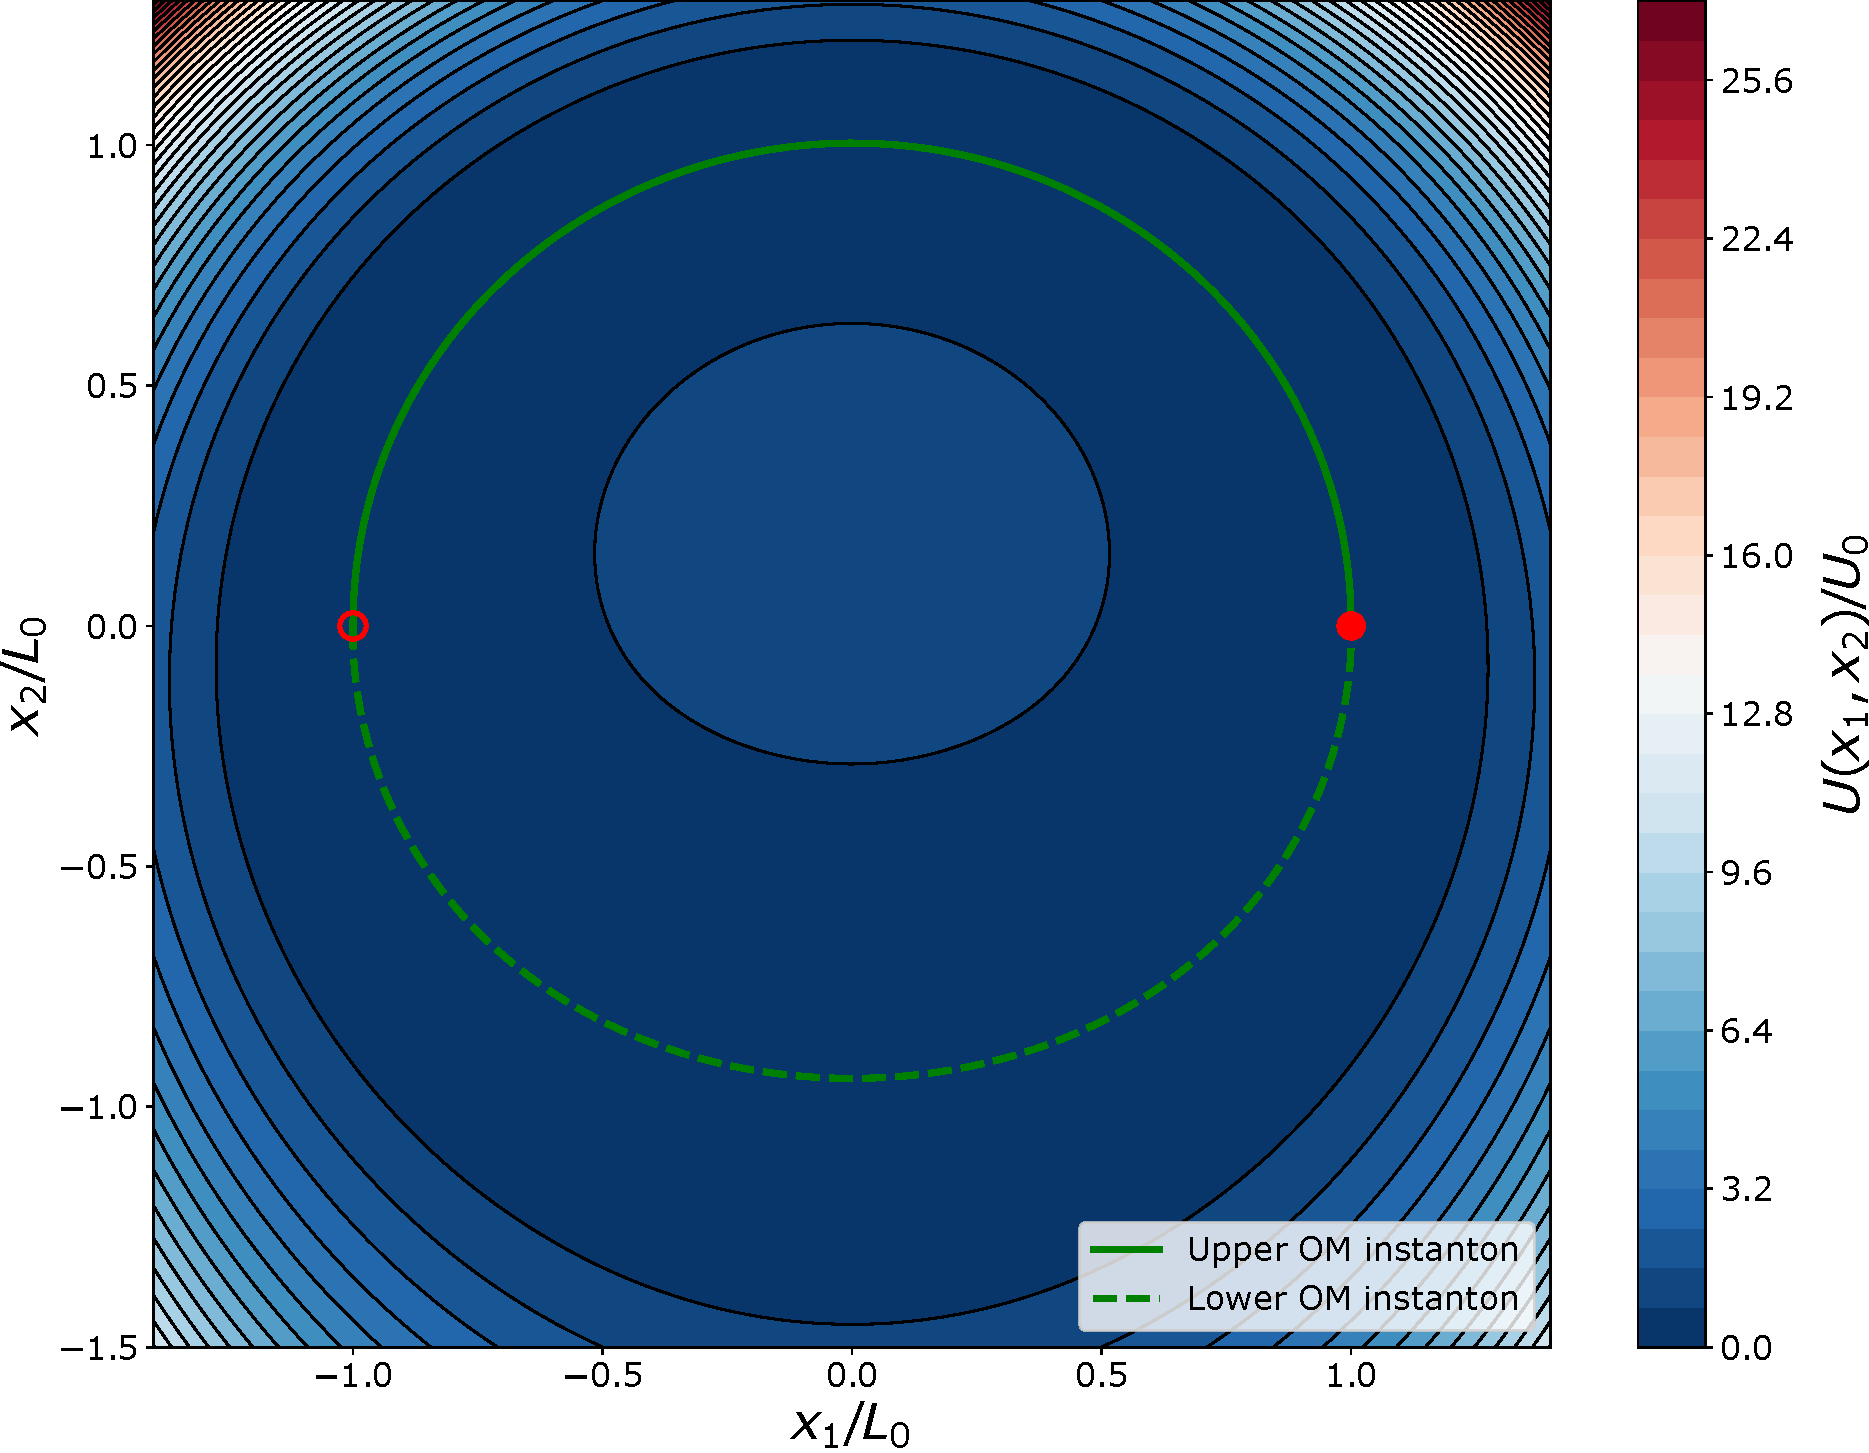
\includegraphics[width=0.6\textwidth]{figs_part1/mcmc/switch_potential}
\centering \caption{The switch potential $U(x_1, x_2)$, defined in Appendix \ref{app:The switch system}. There are two main transition channels between the fixed end-points $\mathbf{x}_0/L_0 = (-1, 0)$ (hollow red circle) and $\mathbf{x}_T/L_0 = (1, 0)$ (filled red circle). The potential has a higher curvature in the upper channel relative to the lower one, which can by seen by the wider contour regions in the lower half of the plot. The upper (green solid line) and lower (green dashed line) local Onsager-Machlup instantons were computed at temperature $\theta/\theta_0 = 0.1$ and duration $T/T_0 = 3$.}
\label{fig:switch potential} 
\end{figure}

As a benchmark problem to test the TMC algorithm on, we have defined a system we call the \textit{switch}. We consider the motion of a particle in a two-dimensional energy landscape given by a potential function. The potential $U(\mathbf{x})$ is a deformed Mexican hat, with a maximum at the origin and a manifold of minima on the circle of radius $L_0$ around the origin. See Fig.~\ref{fig:switch potential} for a plot of $U(\mathbf{x})$, and Appendix \ref{app:The switch system} for a detailed specification of the model. We consider the TPE of paths of duration $T$, which start at $\mathbf{x}_0/L_0 = (-1,0)$ and end at $\mathbf{x}_T/L_0 = (1,0)$. This ensemble features two competing transition channels, namely along the upper and lower semi-circle, which we denote by $\Gamma^{+}$ and $\Gamma^{-}$; by design the potential along $\Gamma^{+}$ is narrower as compared to along $\Gamma^{-}$.

\begin{figure}[t]
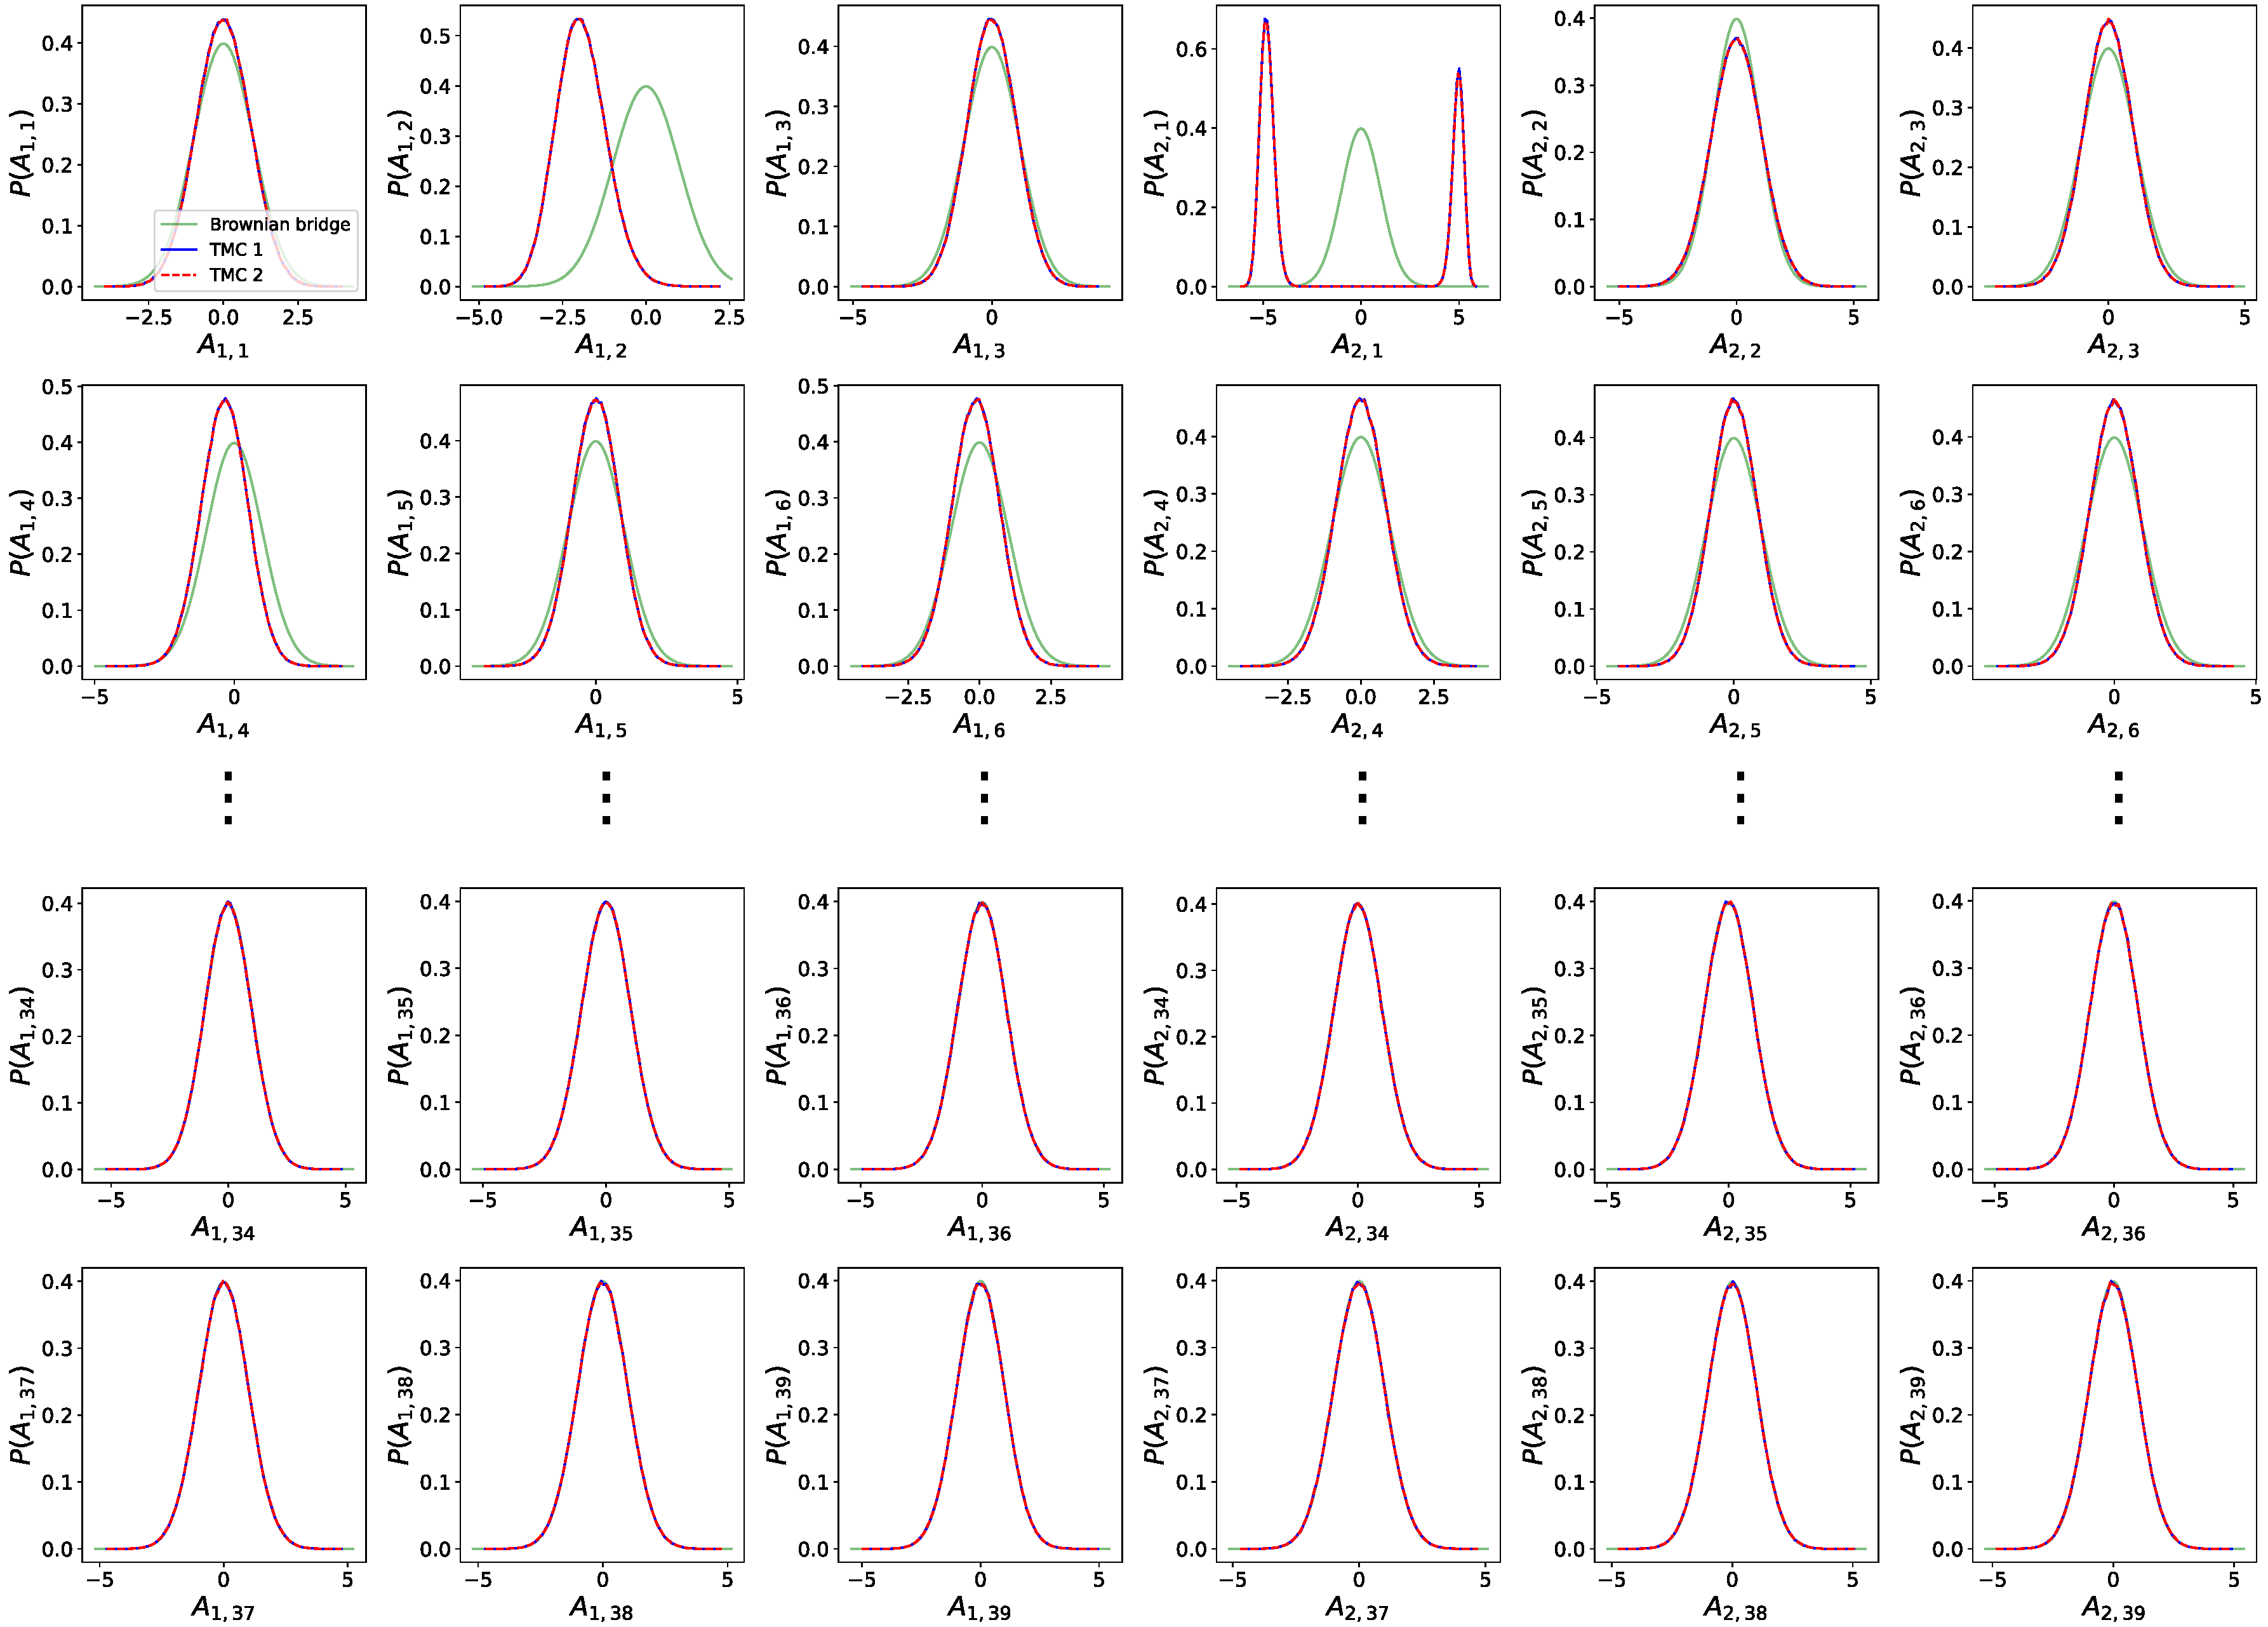
\includegraphics[width=1\textwidth]{figs_part1/mcmc/switch_mode_convergence}
\centering \caption{The marginalised mode distributions of two simulations of the TPE of the switch system using the TMC method with $\theta/\theta_{0}=3.36$ and $T/T_{0}=3$ and $M=10^8$ samples, and the modes of the Brownian bridge process (green solid lines). The first (TMC 1, blue solid lines) was computed using equal teleporter weights $w_+ = w_- = 0.5$ for both channels, and the second (TMC 2, dashed red lines) was biased in favour of the upper channel $w_+ = 0.9, w_- = 0.1$. We see that the mode distributions of the two simulations agree. The mode distribution of $A_{2,1}$ reflects the fact that transition paths concentrate along the upper and lower transition channels.}
\label{fig:switch modes marginalised} 
\end{figure}

\begin{figure}[t]
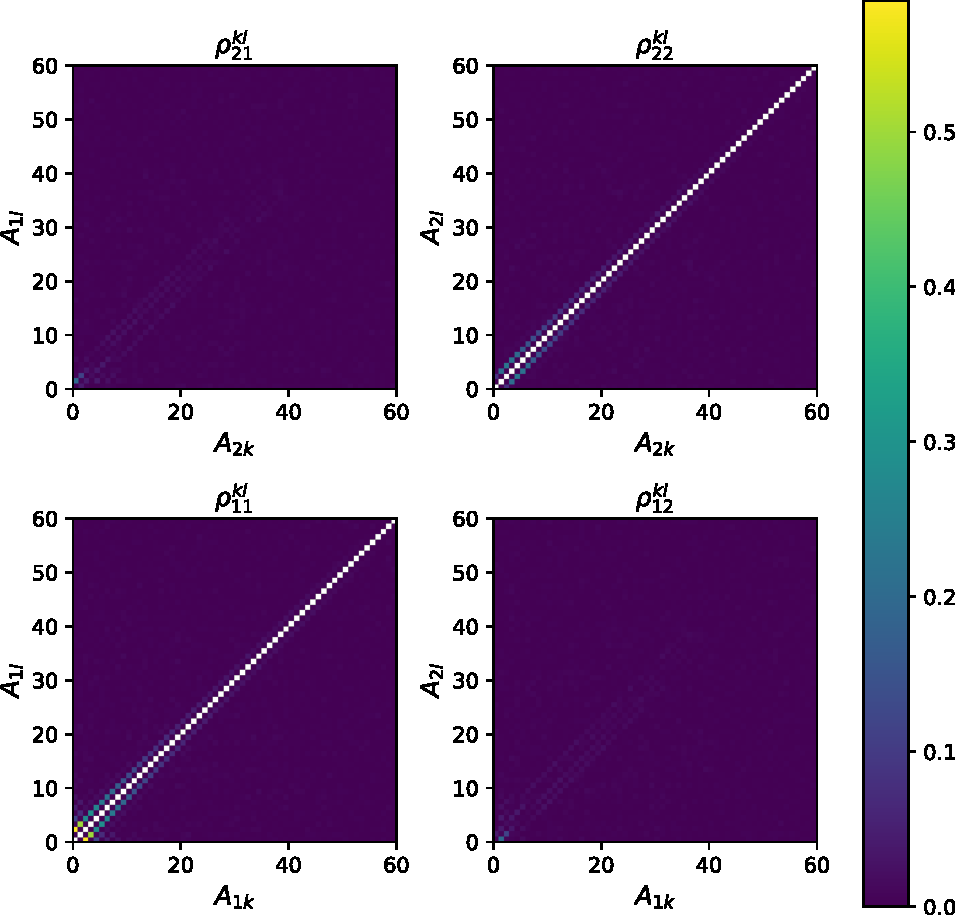
\includegraphics[width=0.8\textwidth]{figs_part1/mcmc/switch_covariance_no_diagonal}
\centering \caption{The absolute normalised covariances $\rho_{ik,jl} = \langle A_{ik} A_{jl} \rangle / \sqrt{ \langle A_{ik}^2 \rangle \langle A_{jl}^2 \rangle }$ of the first $60$ modes of the transition paths of the switch system. As $\rho_{ik,ik} = 1,\ i=1,2,\ k=1,\dots,N$ by definition, we have excluded the diagonals from the plot. We sampled the TPE using the TMC algorithm, with parameters $\theta/\theta_{0}=3.36$, $T/T_{0}=3$ and $N=200(T/T_{0})$ with $M=10^8$ iterations. We see that mode rapidly de-correlate for high mode numberes.}
\label{fig:switch modes covariance} 
\end{figure}

We used the TMC to sample the TPE of the switch system. For temperature $\theta/ \theta_0 = 3.36$ and duration $T/T_0 = 3$, we computed the instantons $\mathbf{x}^{[+]}$ and $\mathbf{x}^{[-]}$ lying in the upper and lower transition channels respectively. We then followed the steps outlined above to implement the TMC. Let $w_+$ and $w_-$ be the teleportation weights of the teleporters of $\mathbf{x}^{[+]}$ and $\mathbf{x}^{[-]}$ respectively. We ran two simulations, with different choice of teleportation weights. In scenario $1$ we used equal weights $w_+ = w_- = 0.5$, and in scenario $2$ we biased in favour of the upper channel $w_+ = 0.9$ and $w_- = 0.1$. The two simulation scenarios lead to the same mode distributions. The results are depicted in Fig.~\ref{fig:switch modes marginalised} and Fig.~\ref{fig:switch modes covariance}. We also see the same spectral band separation we discussed in Sec.~\ref{sec:Mode-space band structure}. Further discussion and analysis of the switch system will be done in Ch.~\ref{ch:Diffusivity dependence of transition paths}, where it will be used to probe the relation between transition channels and diffusivity. The results of Ch.~\ref{ch:Diffusivity dependence of transition paths} will also show that the TMC is robust at low diffusivity regimes, sampling both transition channels, where standard MCMC methods (including the pCN) are intractable.

%As mentioned in the main text, an alternate method to the above would
%be a synthesis of the two sampling approaches in the above algorithm.
%We could replace the reference Wiener measure $\mathbb{P}_{W}$ with
%the mixed Gaussian $\tilde{\mathbb{P}}$, and thus perform the pCN-MCMC
%xwith $\tilde{\mathbb{P}}$ as the invariant measure.

\section{Conclusion}

In this chapter we applied some recent mathematical developments in the field of functional Markov chain Monte Carlo methods to study the transition paths of stochastic processes. We begun with an overview of probability theory over infinite-dimensional sample spaces, and showed that the formal notion of a path-space probability density can be understood rigorously using the classical Wiener measure. Using these mathematical foundations we then described the preconditioned Nicolson-Crank algorithm and used it to sample the transition path ensemble of a general It\^{o} diffusion equation with additive noise.

A suitable reference Gaussian measure of a pinned It\^{o} diffusion is the Brownian bridge process, and we thus expanded transition paths in the Kosambi-Karhunen-Lo\`eve (KKL) basis of the Brownian bridge. We provided numerical and analytical evidence of a band separation in the KKL mode-space of a general It\^{o} diffusion with additive noise. The modes of the KKL expansion decouple in the high-frequency band, and statistically behave indistinguishably from that of Brownian motion. The only non-trivial statistics of an It\^{o} diffusion is thus encapsulated by the joint distributions of the lower-band modes. We used this band separation to construct an adapted step-size for the pCN algorithm, and we demonstrated improved autocorrelation times.

The main result of this chapter was the teleporter MCMC (TMC). In the most general sense, the TMC is a Metropolis-Hastings scheme that interpolates between a given MCMC scheme and an independence sampler, where we called the latter the teleportation measure, and is constructed so that the proposal states concentrate around the maxima of the target measure. Our main innovation was to define such a sampler on the transition path ensembles of It\^{o} processes. Using a semi-classical expansion of the path-probability density, we constructed approximate Gaussian measures around the maxima of the path measure. These formed the basis of the teleportation measure, and the resulting algorithm allowed for sampling TPEs with multiple dominant transition channels.

There are a number of promising future directions. We showed some results that the band separation of It\^{o} processes in KKL mode-space could be exploited to moderately improve autocorrelation times. However, further work can be undertaken to combine the KKL expansion with a multi-level MCMC method \citep{gilesMultilevelMonteCarlo2008, dodwellHierarchicalMultilevelMarkov2015, jansenMultilevelMonteCarlo2020, rohrbachMultilevelSimulationHardsphere2022}. Briefly, we can coarse-grain the system in a series of mode truncations $N_1 < N_2 < \dots N_{M_\text{multi}}$. By running the pCN at the lowest-dimensional chain, we can then upsample via the multi-level scheme to generate samples on the highest-dimensional chain. We would use the band structure of the KKL expansion to engineer upsampling proposals adapted to the system.

Finally, we can consider extending the pCN and TMC to study higher-dimensional settings. The purview of this chapter was the sampling of stochastic transition paths $\mathbf{X}(t)$. Here, $t \in [0, T]$ is an index over a time domain, and the trajectory itself is a map $t \mapsto \mathbf{X}(t)$. In general, we could consider stochastic processes with two or more indices $(t, \mathbf{u}) \mapsto \mathbf{X}(t, \mathbf{u})$, where $\mathbf{u} \in M$ is here a spatial coordinate, that takes values in some $n$-dimensional topological space $M$. Examples of such systems are the stochastic field theories prominent in soft matter physics   \citep{catesTheoriesBinaryFluid2018, tiribocchiActiveModelScalar2015, stenhammarContinuumTheoryPhase2013, wittkowskiScalarF4Field2014, deanLangevinEquationDensity1996}. We will provide a brief sketch of the necessary steps required to sample the transition path ensemble of such systems. As a first example we could consider \textit{Model A} \citep{catesActiveFieldTheories2019}
\begin{equation}
	\partial_t \phi = - \mu \frac{\delta F}{\delta \phi} + \sqrt{2 D} \xi 
\end{equation}
where $\phi = \phi(t, \mathbf{r})$ is a scalar field defined on $M$, $\frac{\delta}{\delta \phi}$ is the functional derivative and $\xi$ is space-time white noise, and $F$ is a free energy functional. A typical choice of $F$ is the $\phi^4$ free energy
\begin{equation}
	F[\phi] = \int_M \left( \frac{a}{2} \phi^2 + \frac{b}{4} \phi^4 + \frac{\kappa}{2} (\nabla \phi)^2 \right) d \mathbf{r}.
\end{equation}
Removing the $\phi^4$ term leads to the \textit{Ohrnstein-Uhlenbeck} (OU) \citep{gardinerHandbookStochasticMethods1990} field equation
\begin{equation} \label{eq:OU process field}
	\partial_t \phi^\text{OU} = - \mu (a \phi^\text{OU} - \nabla^2 \phi^\text{OU}) + \sqrt{2D} \xi.
\end{equation}
Now, if we expand paths in a Fourier basis as $\phi \propto \sum_\mathbf{q} \phi^\text{OU}_\mathbf{q} e^{i \mathbf{q} \cdot \mathbf{r}}$, we get decoupled stochastic equations of motion for each Fourier mode
\begin{equation}
	\partial_t \phi^\text{OU}_\mathbf{q} = - \mu (a + \kappa q^2) \phi^\text{OU}_\mathbf{q} + \sqrt{2D} \xi.
\end{equation}
We see that the Fourier modes of the $\phi^\text{OU}$ process behave like decoupled $1$-dimensional OU processes. Now, it is clear that the OU field is a form of Gaussian process. If we presume that the field-probability measure of a general Model A system has a density with respect the OU field, it would be possible to construct a pCN scheme analogous to the ones describes in this chapter by expanding $\phi$ in the KKL basis of $\phi^\text{OU}$. The latter would require a generalised KKL expansion for fields, which have been discussed in \citep{wangKarhunenLoeveExpansionsTheir2008}, as well as a closed-form expression for the KKL basis of OU bridge processes, which were given here \citep{corlayPropertiesOrnsteinUhlenbeckBridge2014a}.



\chapter{Diffusivity dependence of transition paths} \label{ch:Diffusivity dependence of transition paths}

\section{Introduction}


The fluctuating dynamics of many physical, chemical and biological
systems are commonly modelled by stochastic differential equations
expressed in Langevin or Itô forms \citep{kampenStochasticProcessesPhysics2011a, gardinerStochasticMethodsHandbook2010a, riskenFokkerPlanckEquationMethods2012a, bharucha-reidElementsTheoryMarkov2012a}.
In such systems it is often of great interest to identify the typical
pathways that stochastic paths take to transition from an initial
to a final state, as for example in the nucleation of solids, the
conformational changes in biomolecules, or shifts in ecological balance
\citep{faccioliDominantPathwaysProtein2006a, demarcoPhaseTransitionModel2001a, gardnerConstructionGeneticToggle2000a, mangelBarrierTransitionsDriven1994a, wolynesNavigatingFoldingRoutes1995a, huangMolecularMathematicalBasis2012a, paninskiMostLikelyVoltage2006a, noltingBallsCupsQuasipotentials2016a, leeFindingMultipleReaction2017a}.
Typically, such transition paths cluster around multiple pathways
in the space of configurations and the relative probability of one
or the other of these pathways depends on the drift, the diffusivity,
and the duration allowed for the transition to take place \citep{onsagerFluctuationsIrreversibleProcesses1953a, bachFunctionalsPathsDiffusion1977a, itoProbabilisticConstructionLagrangean1978b, ikedaStochasticDifferentialEquations2014a}.
As transitions are often rare events, direct simulations are not always
practical and other means, analytical or numerical, are required to
study them. Methods that allow for a full exploration of the space
of transition pathways in stochastic dynamical systems, then, are
of substantial theoretical and practical importance.

The theory of large deviations \citep{wentzellSmallRandomPerturbations1970, stratonovichMarkovMethodsTheory1989a, grahamMacroscopicPotentialsBifurcations1989a, arnoldStochasticDifferentialEquations1974a}, the topic of Ch.~\ref{ch:Ritz methods for Freidlin-Wentzel-Graham actions},
provides an analytical method for obtaining transition pathways -
instantons - in regimes dominated by the drift and for very long durations
of path. Experimental systems, however, are typically not in a regime
where the diffusivity is asymptotically low and durations are asymptotically
long \citep{gladrowExperimentalMeasurementRelative2021a}. While the
relevance of including finite-temperature fluctuations around the
instanton \citep{gelfandIntegrationFunctionalSpaces1960a} is increasingly
recognized \citep{nickelsenNoiseCorrectionLarge2022, corazzaNormalizedGaussianPath2020b, luGaussianApproximationsTransition2017a},
the physical implications of these fluctuations are far from being
understood.

In this chapter, we show that the competition between drift and diffusion
in transition pathways can be studied using the semi-classical expansions
of the path measure of the stochastic dynamics introduced in Sec.~\ref{sec:Teleporter MCMC}. We use a mixture of
Gaussian measures to approximate the path measure around its local
instantons. This allows us to demarcate and transcend the boundaries
of the low diffusivity regime, without recourse to sampling the TPE directly using MCMC methods. We demonstrate this explicitly for
a two-dimensional overdamped mechanical system, with both conservative
and non-conservative forces. For this system we uncover a counterintuitive
phenomenon where typical transition paths do not concentrate around
the most probable path, even at low-to-intermediate diffusivities
where the Gaussian approximation is still valid. To validate our results
numerically, and to study the TPE at high-diffusivity regimes, we use the teleporter MCMC (TMC) method developed in Ch.~\ref{ch:Monte Carlo methods in Path Spaces},
that allows for simultaneous exploration of multiple transition pathways. We
find excellent agreement between the semi-classical expansion and
numerical results for a large range of diffusivities and path durations.
We now detail our results.

\section{The transition path ensemble}

The general class of systems in consideration is the $d$-dimensional overdamped Langevin equation with additive noise, which we write here again in Itô form as
\begin{equation} \label{eq:ito equation again}
d\mathbf{X}=\mu\mathbf{F}dt+\sqrt{2D}d\mathbf{W}. 
\end{equation}
This represents the stochastic displacement $d\mathbf{X}$ in a time
interval $dt$ of a particle with coordinate $\mathbf{X}$ subject
to a force field $\mathbf{F}$ and Brownian displacements $\sigma d\mathbf{W}$,
where $\mathbf{W}$ is the Wiener process. The particle mobility is
$\mu$, the diffusion constant is $D=\mu/\beta$, and the temperature
is $\theta$ with $\beta^{-1}=k_{B}\theta$, and $k_{B}$ the Boltzmann
constant. We are interested in realisations $\mathbf{X}(t)$ of Eq.~\ref{eq:ito equation again}
that are of duration $T$ and have fixed terminii $\mathbf{X}(0)=\mathbf{x}_{0}$
and $\mathbf{X}(T)=\mathbf{x}_{T}$. These trajectories form the set
of continuous paths that we have called the transition path ensemble (TPE), and denote as $E_{\mathbf{x}_0}^{\mathbf{x}}([0,T])$. We will study the temperature dependence of the TPE using both the TMC algorithm presented in Ch.~\ref{ch:Monte Carlo methods in Path Spaces}, as well as the semi-classical approximation of the path-probability measure, which are developed in Sec.~\ref{sec:Semi-analytical approximations of stochastic path measures}.

\subsection{Model system}

The methods we will develop in subsequent sections will be applied on the \textit{switch} system, which was previously used in Sec.~\ref{sec:TMC Numerical algorithm}, and is defined in detail in Appendix \ref{app:The switch system}.
The model consists of a particle in $d=2$ dimensions in a potential force field $\mathbf{F}=-\nabla U(\mathbf{x})$, depicted in Fig.~\ref{fig:switch potential} and Fig.~\ref{fig:switch trajectories}.
The potential $U(\mathbf{x})$ has two prominent transition channels, the upper and lower semi-circular channels which we denote as $\Gamma^{+}$ and $\Gamma^{-}$ respectively. The potential has a continuous manifold of minima along $\Gamma^{+}$ and $\Gamma^{-}$, such that the purely energetic cost of traversing either channel is the same. However, by design the potential has a larger curvature along $\Gamma^{+}$ relative to $\Gamma^{-}$. Therefore, the lower channel is wider than the upper channel, as can be seen in Fig.~\ref{fig:switch potential}. As an additional model, we add a non-conservative circular force $\mathbf{F}^{a}$ to the switch system. This force works as a bias in favour of the upper channel, by decreasing the energetic cost of traversing it, and increases the energetic cost of the lower channel. The models have been constructed so as to study the interplay between the deterministic drift and diffusivity.

\section{Semi-analytical approximations of stochastic path measures} \label{sec:Semi-analytical approximations of stochastic path measures}

Here we derive an approximation of the path measure $\mathbb{P}_\mathbf{X}$ of the It\^{o} diffusion process with additive noise. In Sec.~\ref{sec:The Gaussian mixture approximation} we construct a global approximation of $\mathbb{P}_\mathbf{X}$ using a weighted sum of the Gaussian distributions derived in Sec.~\ref{sec:Second-order variational expansions of stochastic action functionals}, where the latter approximated the path measure around given local instantons. We then use this result in Sec.~\ref{sec:Second-order variational expansions of stochastic action functionals} to derive estimates of transition channel probabilities, which serve as a measure for the concentration of the TPE around a given transition channel. Our method is a combination of the semi-classical approach to study path-integrals \citep{chaichianPathIntegralsPhysics2001, schulmanTechniquesApplicationsPath1996, smirnovEstimationPathIntegral2010, moretteDefinitionApproximationFeynman1951, marinovPathIntegralsQuantum1980, sakuraiModernQuantumMechanics2017} and a standard technique in statistical data analysis \citep{gelmanBayesianDataAnalysis, scottMultivariateDensityEstimation2015, goodfellowDeepLearning2016, nguyenApproximationFiniteMixtures2020, carreira-perpinanModefindingMixturesGaussian2000}, wherein a target probability measure is estimated as Gaussian mixture distribution. 

We will begin by first giving some intuition by drawing an analogy in the one-dimensional case. For a one-dimensional probability density $p(x)=\mathcal{Z}^{-1}\exp(-V(x))$,
where $\mathcal{Z}$ is a normalization constant and where the potential
$V(x)$ has well-separated relative minima $x_{\alpha},\ \alpha=1,\dots,K$,
we can approximate $p(x)$ around $x_{\alpha}$ using a Gaussian
approximation
\begin{equation}
p(x)\approx\frac{1}{\mathcal{{Z}}}e^{-V(x_{\alpha})-V''(x_{\alpha})(x-x_{\alpha})^{2}/2}=:\frac{{{\mathcal{Z}}_{\alpha}}}{\mathcal{{Z}}}e^{-V(x_{\alpha})}p^{[\alpha]}(x)\label{eq:local approximation of rho}
\end{equation}
with a normalised Gaussian distribution $p^{[\alpha]}(x):=\mathcal{Z}_{\alpha}^{-1}e^{-V''(x_{\alpha})(x-x_{\alpha})^{2}/2}$
and where $\mathcal{Z}_{\alpha}=\sqrt{2\pi/V''(x_{\alpha})}$. Equation
\ref{eq:local approximation of rho} is a local approximation of $p(x)$
around $x_{\alpha}$. If $p(x)$ is highly peaked around its maxima
(for example if $V(x)$ describes a Boltzmann distribution $V(x)=U(x)/(k_{B}\theta)$
at a low temperature $\theta$), a global approximation of $p(x)$
is the Gaussian mixture
\begin{equation} 
p(x)\approx \sum_{\alpha=1}^{K}\omega_{\alpha}p^{[\alpha]}(x)\label{eq:one_dimensional_sum_of_gaussians}
\end{equation}
where $\omega_{\alpha}=e^{-V(x_{\alpha})}\mathcal{Z}_{\alpha}/ \sum_{\gamma=1}^{K}e^{-V(x_{\gamma})}\mathcal{Z}_{\gamma}$ are constants that weight the local Gaussian distributions. The weight $\omega_\alpha$ is the size of the support of $p^{[\alpha]}$ relative to the other local Gaussian. From Eq.~\ref{eq:one_dimensional_sum_of_gaussians} we see that the support of $p^{[\alpha]}$ is determined by an interplay of the `peak' of the distribution $e^{-V(x_{\alpha})}$, and the `width', which is measured by the normalisation constant $\mathcal{Z}_{\gamma}$.

Equation \ref{eq:one_dimensional_sum_of_gaussians} can be used
to approximately evaluate any expectation value. In particular, the
probability of being in well $\alpha$ (i.e.~around $x_{\alpha}$)
is given by
\begin{align}
\mathbb{P}(x\in\text{{well\,}}\alpha) & = \langle \chi_{\alpha} \rangle =\int_{-\infty}^{\infty}dx\,\chi_{\alpha}(x)p(x)\approx\sum_{\beta=1}^{K}\omega_{\beta}\int_{-\infty}^{\infty}dx\,\chi_{\alpha}(x)p^{[\beta]}(x)\\
 & \approx w_{\alpha}\int_{-\infty}^{\infty}dx\,p^{[\alpha]}(x)=\omega_{\alpha}=\frac{{e^{-V(x_{\alpha})}\mathcal{Z}_{\alpha}}}{\sum_{\gamma=1}^{L}e^{-V(x_{\gamma})}\mathcal{Z}_{\gamma}},\label{eq:one_dimensional_well_probability}
\end{align}
where the indicator function $\chi_{\alpha}(x)$ is 1 if $x$ is in
well $\alpha$ and zero otherwise, and where we assume that the potential
wells of $V(x)$ are well-separated so that $\chi_{\alpha}(x)p^{[\beta]}(x)$
is negligibly small whenever $\alpha\neq\beta$. In the following we apply the same steps as above to the case of the TPE. 

\subsection{The Gaussian mixture approximation} \label{sec:The Gaussian mixture approximation}

We use the quadratic expansion of the stochastic action derived in Sec.~\ref{sec:Second-order variational expansions of stochastic action functionals} to construct an approximate probability measure over the TPE. Let $\mathbf{x}^{[\alpha]},\alpha=1,\dots,K$ be the local instantons of a given Langevin system. For each local instanton we have the Gaussian measures $\mathbb{P}_G^{[\alpha]}$ with mean $\mathbf{x}^{[\alpha]}$ and precision operators $\mathcal{H}^{[\alpha]}$, which locally approximates the path measure around $\mathbf{x}^{[\alpha]}$. We use these local approximants to construct a Gaussian mixture measure with density
\begin{equation} \label{eq:gaussian mixture approx of TPE}
	\tilde{P}_\mathbf{X}[\mathbf{X}] = \sum_{\alpha=1}^K \omega_\alpha \exp \left( - \frac{1}{2} \langle \mathbf{X} - \mathbf{x}^{[\alpha]}, \mathcal{H}^{[\alpha]} (\mathbf{X} - \mathbf{x}^{[\alpha]}) \right)
\end{equation}
with corresponding measure $\tilde{P} \sim \tilde{P}$. We now impose that $\tilde{P}_\mathbf{X}[\mathbf{x}^{[\alpha]}] = P_\mathbf{X}[\mathbf{x}^{[\alpha]}]$ for each $\alpha = 1,\dots,K$. We get
\begin{equation} \label{eq:gaussian mixture approx weights}
	\omega_\alpha = \frac{e^{-S_{\text{OM}}[\mathbf{x}^{[\alpha]}]} (\mathcal{Z}^{[\alpha]} / \mathcal{Z}_\mathbf{B}) }{ \sum_{\gamma=1}^{K}e^{-S_{\text{OM}}[\mathbf{x}^{[\gamma]}]}(\mathcal{Z}^{[\gamma]} / \mathcal{Z}_\mathbf{B}) }
\end{equation}
where $\mathcal{Z}^{[\alpha]}$ and $\mathcal{Z}_\mathbf{B}$ formally represent the normalisation constants for the path-densities for the It\^{o} process and Brownian bridge process respectively. Whilst divergent on their own, their ratio $\mathcal{Z}^{[\alpha]} / \mathcal{Z}_\mathbf{B}$ is finite, and we derive a formula with which to compute them in Appendix \ref{app:Calculation of the Gaussian normalisation constants}. The measure $\tilde{\mathbb{P}}_\mathbf{X}$ serves as an approximation of the true path-measure $\mathbb{P}_\mathbf{X}$. The underlying assumption is that $\mathbb{P}_\mathbf{X}$ concentrates around its local instantons. In sufficiently low diffusivity-regimes, $\tilde{\mathbb{P}}_\mathbf{X}$ will be a good approximation for $\mathbb{P}_\mathbf{X}$.

The sequences of steps taken to construct Eq.~\ref{eq:gaussian mixture approx of TPE} is standard technique from statistical data analysis \citep{gelmanBayesianDataAnalysis, scottMultivariateDensityEstimation2015, goodfellowDeepLearning2016, nguyenApproximationFiniteMixtures2020, carreira-perpinanModefindingMixturesGaussian2000}, where we have applied it here in the infinite-dimensional path-space setting.

\subsection{Approximations of transition channel probabilities} \label{sec:Approximations of transition channel probabilities}

We now derive estimates of transition channel probabilities using the Gaussian mixture approximation of the TPE $E_{\mathbf{x}_0}^{\mathbf{x}}([0,T])$. Let $E^{[\alpha]} \subset E_{\mathbf{x}_0}^{\mathbf{x}}([0,T]),\ \alpha=1,\dots,J$,
which are disjoint open sets in the TPE, be the $J$ transition channels
under consideration. We define
\begin{equation} \label{eq:transition channel prob}
	\rho^{[\alpha]}(\theta,T)=\mathbb{P}_\mathbf{X}[E^{[\alpha]}]
\end{equation}
which is the probability of observing a transition path $\mathbf{X} \in E_{\alpha} \subset E_{\mathbf{x}_0}^{\mathbf{x}}([0,T])$. The quantity $\rho^{[\alpha]}(\theta,T)$ can be seen as an observable, and the expectation on the right-hand side of Eq.~\ref{eq:transition channel prob} will be computed by sampling the TPE using MCMC methods. However, here we will also approximate $\rho^{[\alpha]}(\theta,T)$ using the Gaussian mixture measure as
\begin{equation} \label{eq:transition channel prob approx}
	\rho^{[\alpha]}(\theta,T) \approx \rho_G^{[\alpha]} \equiv \tilde{\mathbb{P}}_\mathbf{X}[E^{[\alpha]}]
\end{equation}
where we have defined the approximate transition channel probability $\rho_G^{[\alpha]}$.

At sufficiently low temperatures we can assume that $\mathbb{P}_\mathbf{X}(\cup_{\alpha} E^{[\alpha]})\approx 1$, i.e. approximately all stochastic paths travel via one of the
transition channels. We also assume that the transition channels concentrate around the local instantons of the path measure. That is, $J = K$, where $K$ is the number of local instantons, and that $\mathbf{x}^{[\alpha]}\in E_{\alpha}$. Furthermore, we assume that each local Gaussian approximate measure $\mathbb{P}_G^{[\alpha]}$ lacks support on transition channels other than $E^{[\alpha]}$, that is $\mathbb{P}_G^{[\alpha]}(U_{\gamma \neq \alpha} E^{[\gamma]}) \approx 0$. Under these assumptions $\rho^{[\alpha]}(\theta,T)$ is well-approximated by $\rho_G^{[\alpha]}$, and we have
\begin{equation} \label{eq:approx transition channel prob}
\rho_G^{[\alpha]}(\theta,T) = w_{\alpha} = \frac{e^{-S_{\text{OM}}[\mathbf{x}^{[\alpha]}]} (\mathcal{Z}^{[\alpha]} / \mathcal{Z}_\mathbf{B}) }{ \sum_{\gamma=1}^{K}e^{-S_{\text{OM}}[\mathbf{x}^{[\gamma]}]}(\mathcal{Z}^{[\gamma]} / \mathcal{Z}_\mathbf{B}) }
\end{equation}
According to Eq.~\ref{eq:approx transition channel prob} the relative channel probabilities are determined by an interplay between the instanton probabilities, as quantified by $e^{-S_{\text{OM}}[\mathbf{x}^{[\alpha]}]}$, and the amplitudes of the Gaussian fluctuations around the local instantons, measured by $\mathcal{Z}^{[\alpha]}/ \mathcal{Z}_\mathbf{B}$. We see that it is possible for a transition channel to be dominant despite its local instanton having a low probability, if the `width' $\mathcal{Z}^{[\alpha]}/ \mathcal{Z}_\mathbf{B}$ compensates for it. It is instructive to compare $\rho_G^{[\alpha]}(\theta,T)$  with another estimator
\begin{equation}
	\rho_{I}^{[\alpha]}(\theta,T)=e^{-S_{\text{OM}}[\mathbf{x}^{[\alpha]}]}/\sum_{\gamma}e^{-S_{\text{OM}}[\mathbf{x}^{[\gamma]}]}
\end{equation}
in which only the instanton probabilities are retained.

To use Eq.~\ref{eq:approx transition channel prob} in practice, we retrieve the instantons
$\mathbf{x}^{[\alpha]}$ using a Ritz variational method as discussed in Ch.~\ref{ch:Ritz methods for Freidlin-Wentzel-Graham actions}. We subsequently evaluate the regularised normalisation constants $\mathcal{Z}^{[\alpha]} / \mathcal{Z}_\mathbf{B}$ using the method described in Appendix \ref{app:Calculation of the Gaussian normalisation constants}. Note that the instantons $\mathbf{x}^{[\alpha]}$ and the regularised normalisations $\mathcal{Z}^{[\alpha]} / \mathcal{Z}_\mathbf{B}$ are both dependent on $\theta$ and $T$.

\begin{comment}
\section{Numerical experiments}

To infer the range of
validity of our semi-analytical approximation it is necessary to compare
Eq.~\ref{eq:r function} with numerical simulations. In parameter
regimes where transitions are very rare, it is not feasible to sample
the TPE using direct simulations. We therefore numerically probe the
TPE using a MCMC algorithm built on the \textit{preconditioned Crank-Nicholson
algorithm }\textit{\emph{(pCN) }}\citep{cotterMCMCMethodsFunctions2013a,beskosMCMCMETHODSDIFFUSION2008a,hairerSpectralGapsMetropolis2014a},
as detailed in the SI \citep{note:SI}. In essence, we approximate
the function space of all transition paths by a finite sum of basis
functions \citep{kosambiStatisticsFunctionSpace1943,karhunenUberLineareMethoden1947,loeveProbabilityTheory1977},
and perform a random walk on the resulting finite-dimensional space
of basis coefficients; the random walk is designed such that the resulting
transition path samples are distributed according to the TPE we seek
to probe.

A general shortcoming of MCMC methods and also other transition path
sampling techniques \citep{bolhuisTransitionPathSampling2002a,bolhuisTransitionPathSampling,dellagoTransitionPathSampling1998a,dellagoEfficientTransitionPath1998a,fujisakiOnsagerMachlupActionbased2010}
is that when the distribution to be sampled is multimodal with regions
of low probability in between the modes, it may take prohibitively
long to obtain converged results. For overdamped Langevin dynamics
Eq.~\ref{eq:ito equation}, this corresponds to medium-to-low temperature
regimes in systems with competing transition pathways, where the TPE
concentrates around the local instantons. One way to overcome this
issue is to use replica exchange \citep{fujisakiOnsagerMachlupActionbased2010},
which requires running several instances of the MCMC algorithm at
varying temperatures. Here we introduce a modification of the pCN-MCMC
that operates only at one temperature, which we call the \emph{Teleporter
MCMC }(TMC), which utilises the Gaussian mixture approximation of
the TPE. At each step of the TMC there is a small probability to jump
between the transition channels, which accelerates mixing between
them. We provide a detailed description of the algorithm in the SI
\citep{note:SI}.
\end{comment}

\section{Results}

\begin{figure*} 
    \centering
     
    \begin{subfigure}[b]{0.7\textwidth}
        \centering
        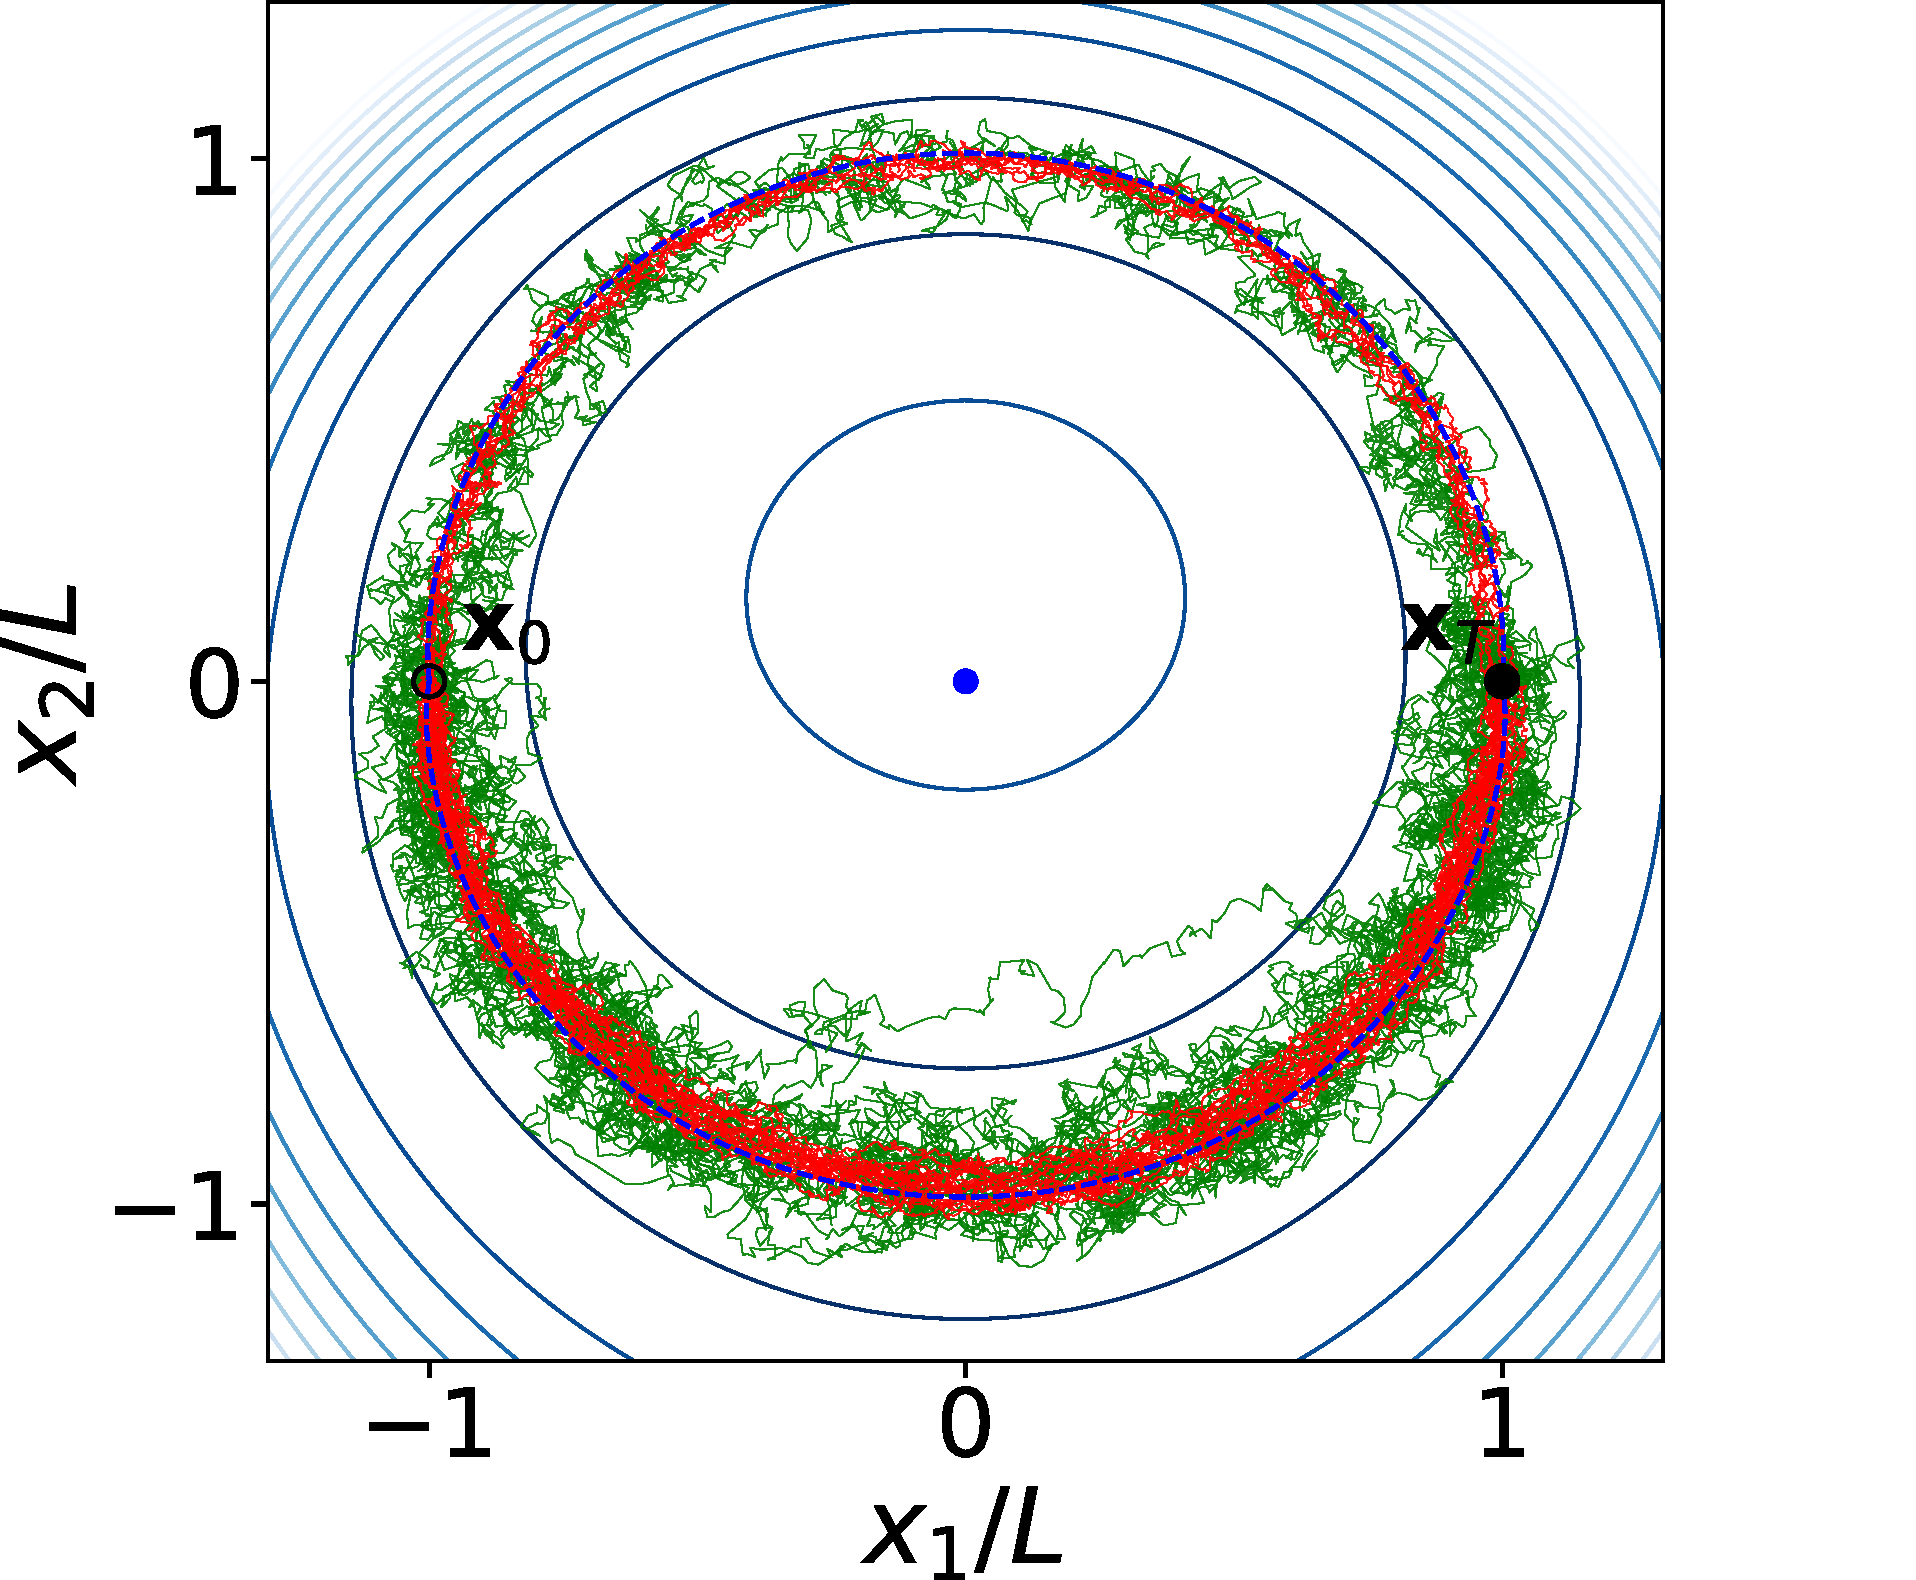
\includegraphics[width=\textwidth]{figs_part1/mcmc/switch_trajectories_without_force}
        \caption[]%
        {}    
        \label{fig:switch trajectories}
    \end{subfigure}
     
     \vskip\baselineskip  
     
    \begin{subfigure}[b]{0.495\textwidth}  
        \centering 
        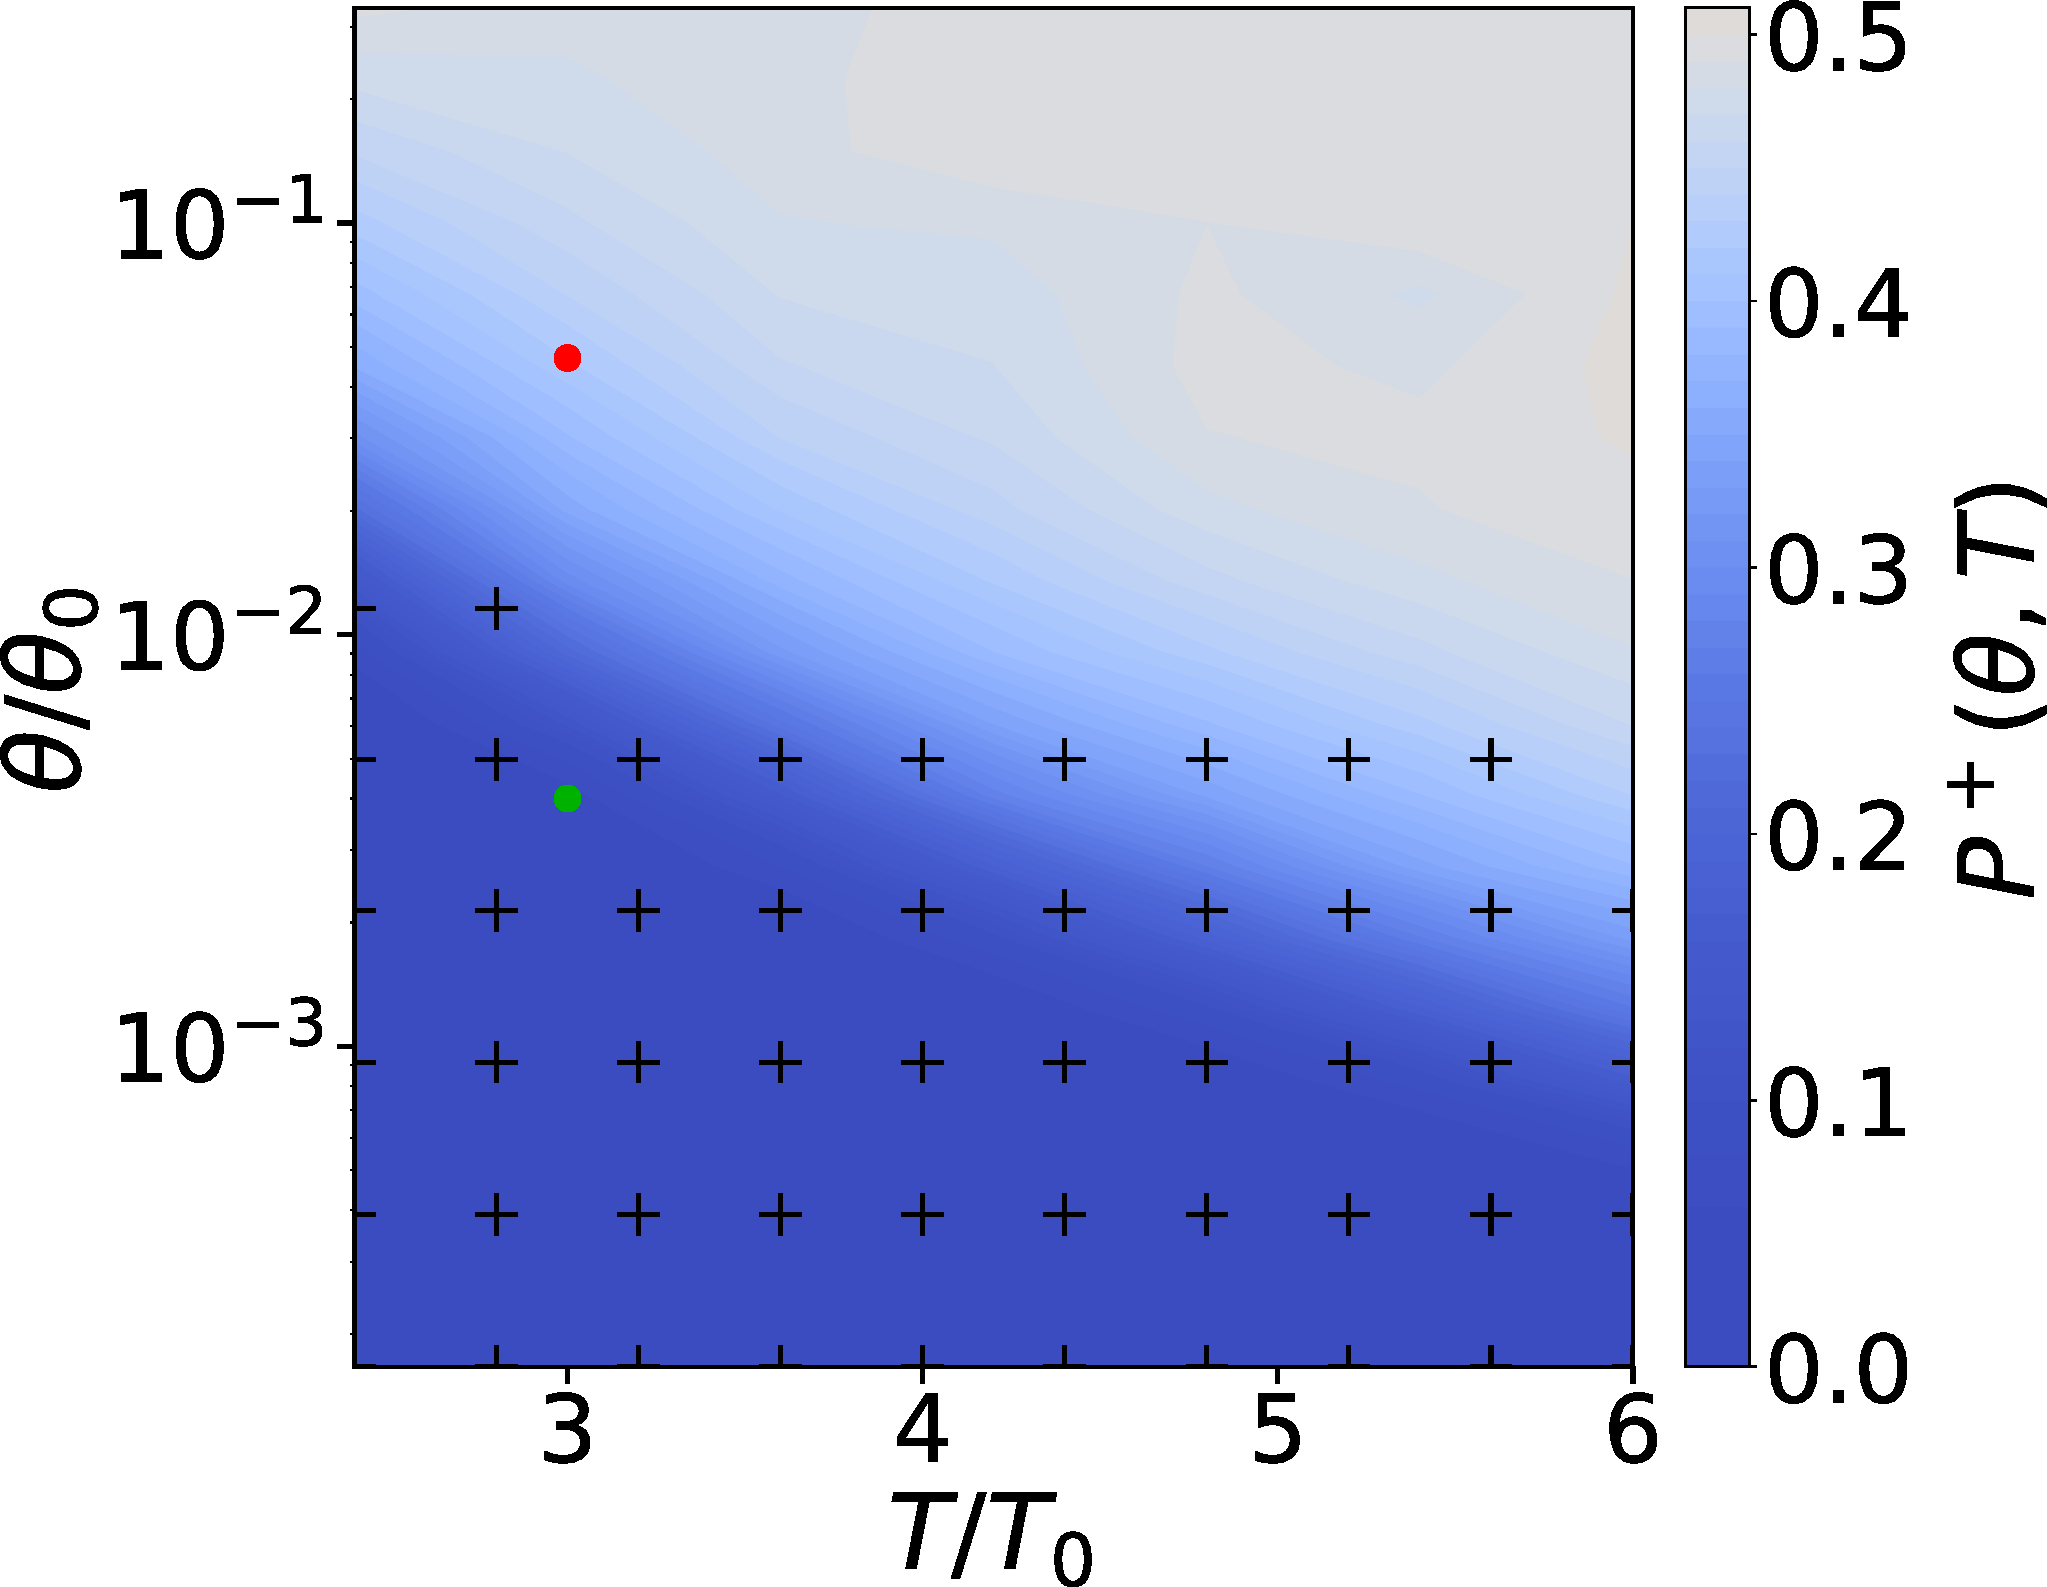
\includegraphics[width=\textwidth]{figs_part1/mcmc/switch_channel_rates}
        \caption[]%
        {}    
        \label{fig:switch channel rates}
    \end{subfigure}
    \hfill
    \begin{subfigure}[b]{0.475\textwidth}
        \centering
        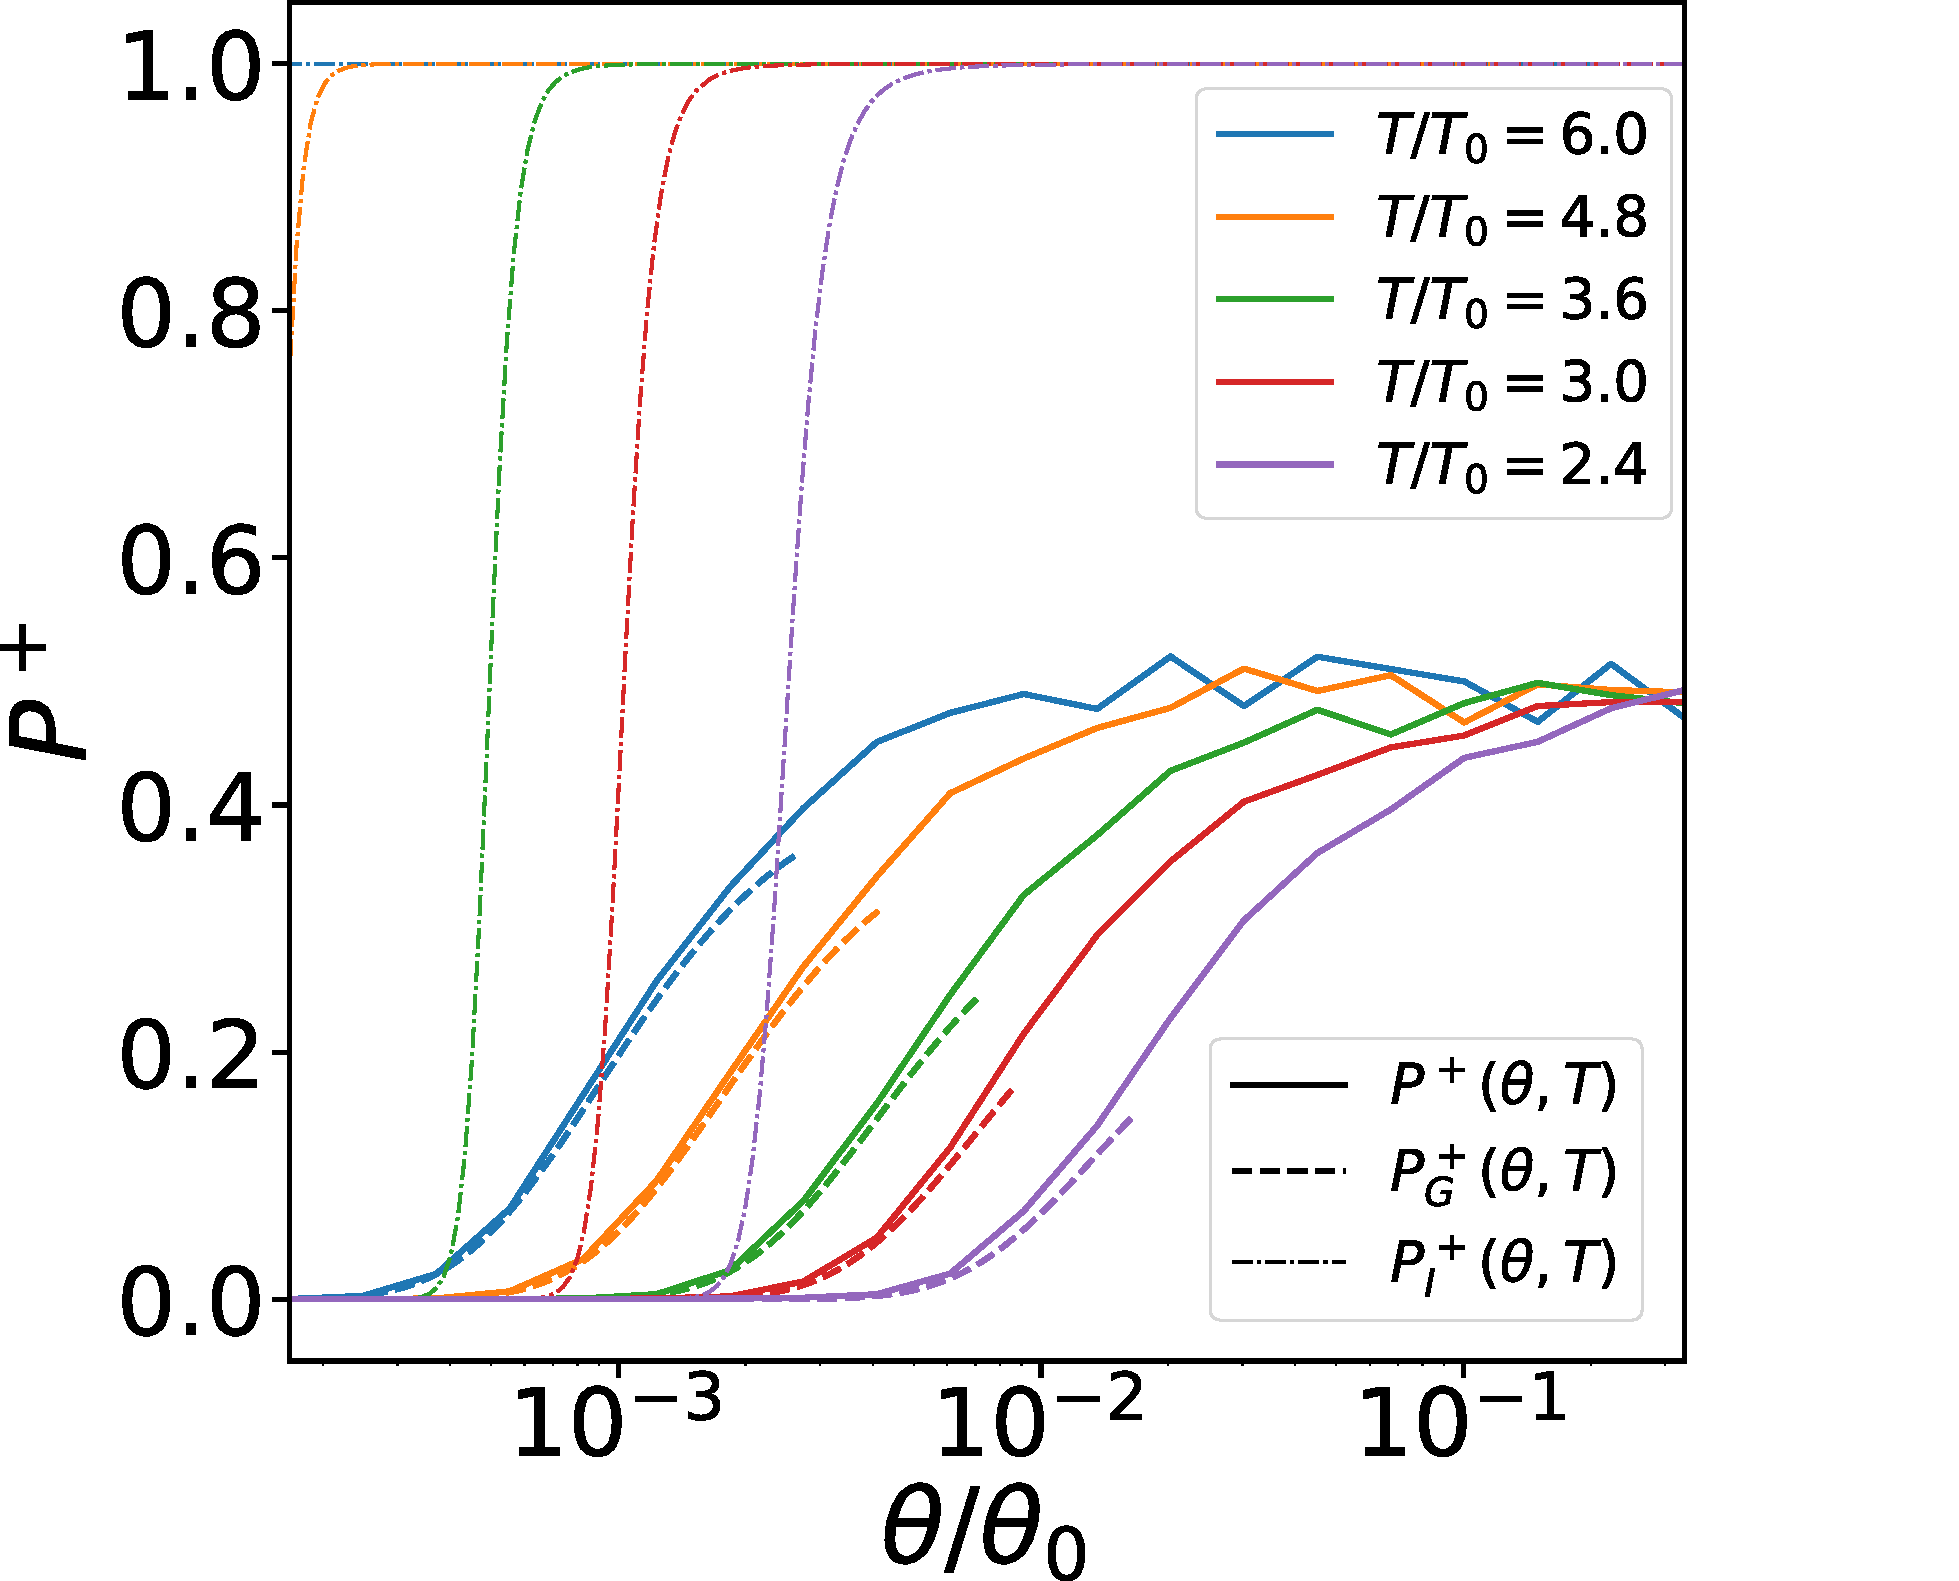
\includegraphics[width=\textwidth]{figs_part1/mcmc/switch_channel_rates_line_plot}
        \caption[]%
        {}    
        \label{fig:switch line plots}
    \end{subfigure}     

    \caption[  ]
    {\small Diffusivity-dependence of the transition path ensemble for the conservative
switch system. Panel (a) shows 50 stochastic trajectories sampled using
the TMC method for overdamped dynamics in the potential
$U(x)$ (see Appendix \ref{app:The switch system}). The dashed blue (green) lines are upper
(lower) instantons between initial (circle, $\mathbf{x}_{0}$) and
final (filled circle, $\mathbf{x}_{T}$) points. Upper and lower channels
are equally populated at temperature $\theta/\theta_{0}=0.047$ (green)
but the lower channel is preferred at the lower temperature $\theta/\theta_{0}=0.004$
(red). Trajectories of duration $T/T_{0}=3$ are sampled with $N=200(T/T_{0})$
modes. Panel (b) is a pseudocolor plot quantifying the variation of
the upper channel probability $\rho_{G}^{+}$ with temperature and duration,
as obtained from TMC. The plus signs show regions where the Gaussian
mixture approximation $\rho_{G}^{+}$, defined in Eq.~\ref{eq:approx transition channel prob}, is within
a $5\%$ margin of error of the simulated value. The red and green
dots correspond to the same color-coded simulations in panel (a).
Panel (c) compares the upper channel probability $\rho^{[\alpha]}(\theta,T)$, computed using the TMC, with the Gaussian mixture and
instanton approximations to the upper channel probability as function
of temperature for a range fixed durations of path $T$.} 
\end{figure*} 

\begin{comment}
\begin{figure*} 
    \centering
  
    \begin{subfigure}[b]{0.31\textwidth} 
        \centering 
        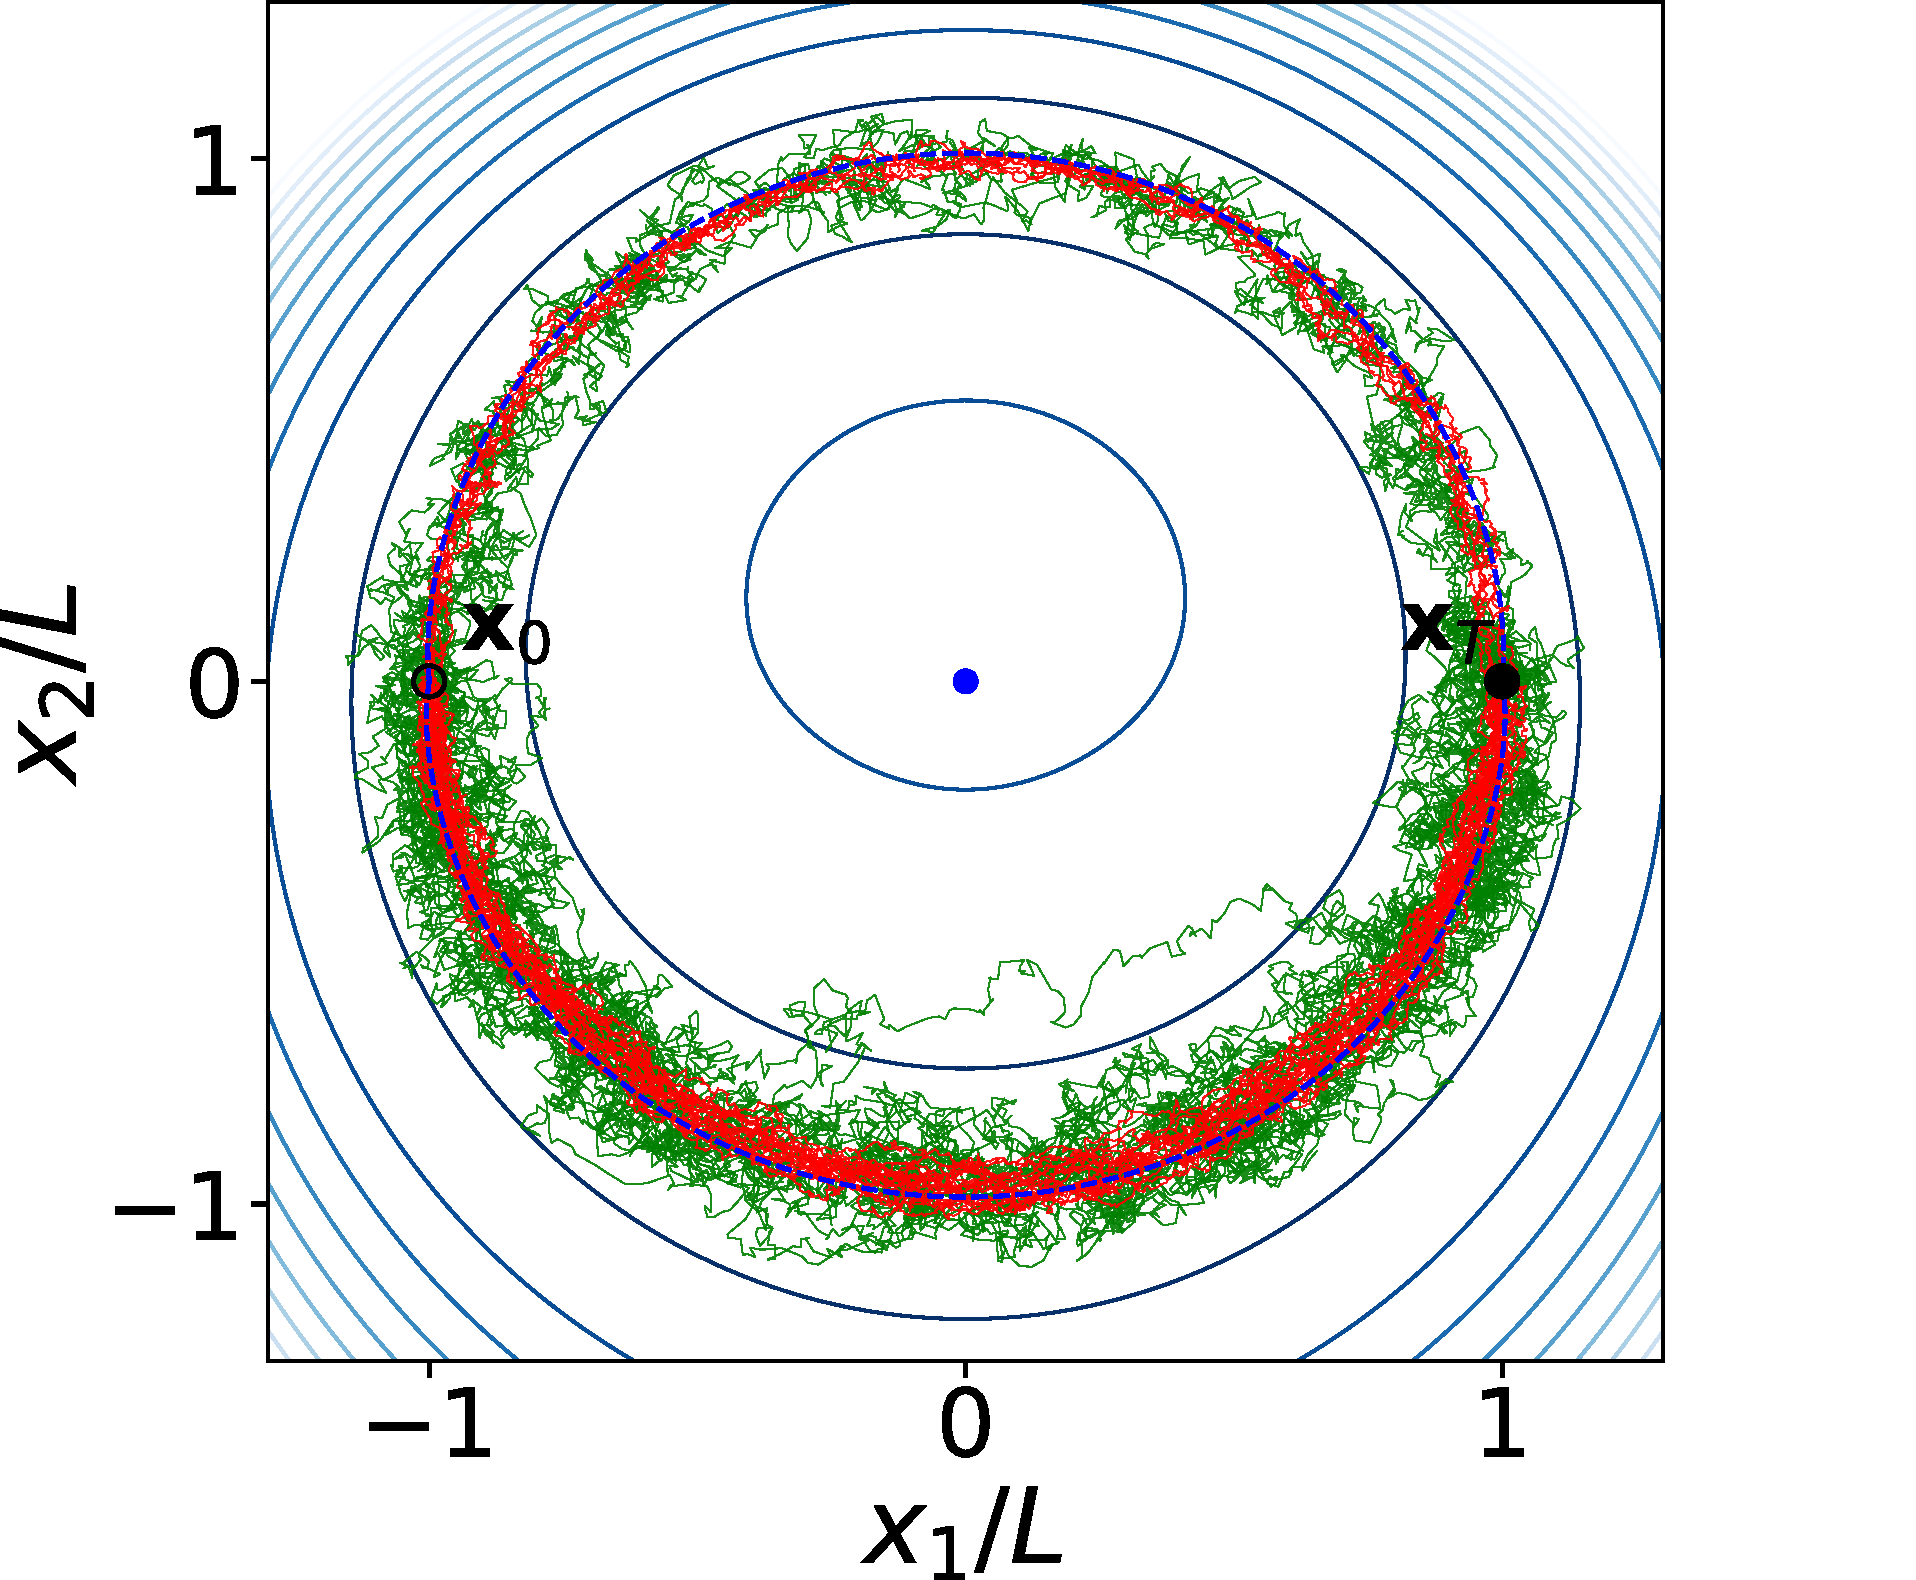
\includegraphics[width=\textwidth]{figs_part1/mcmc/switch_trajectories_without_force}
        \caption[]%
        {}      \label{fig:switch trajectories}
    \end{subfigure}
    \hfill
    \begin{subfigure}[b]{0.33\textwidth}
        \centering
        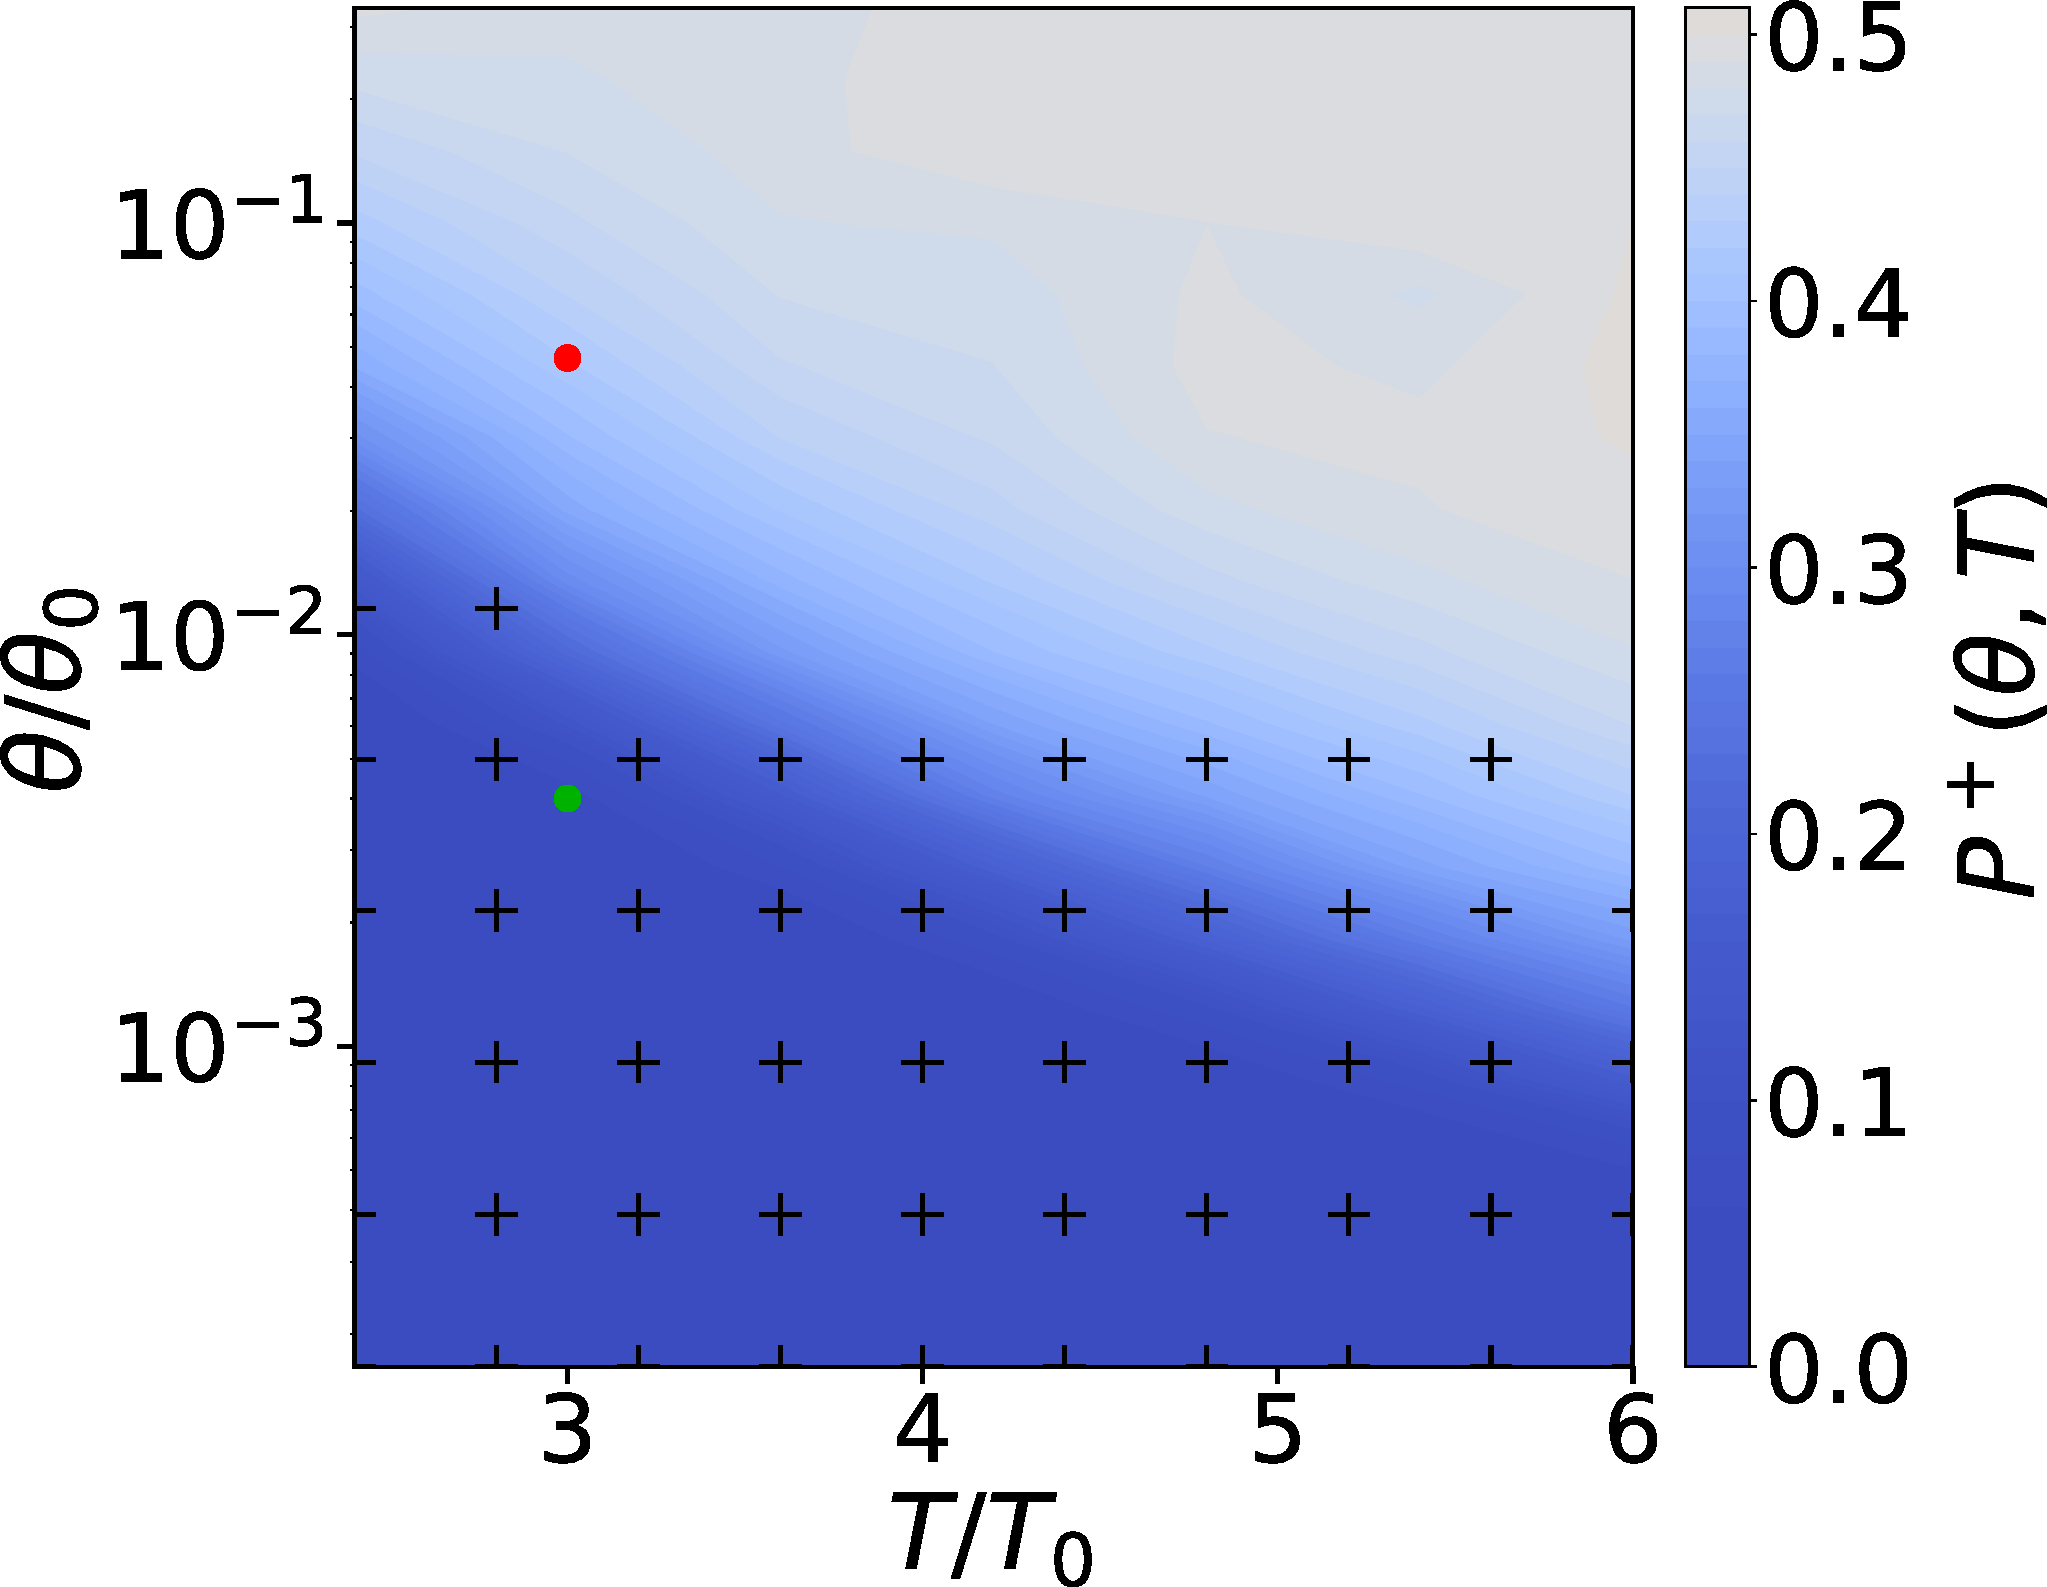
\includegraphics[width=\textwidth]{figs_part1/mcmc/switch_channel_rates}
        \caption[]%
        {}    
    \end{subfigure}    
    \hfill
    \begin{subfigure}[b]{0.314\textwidth}
        \centering
        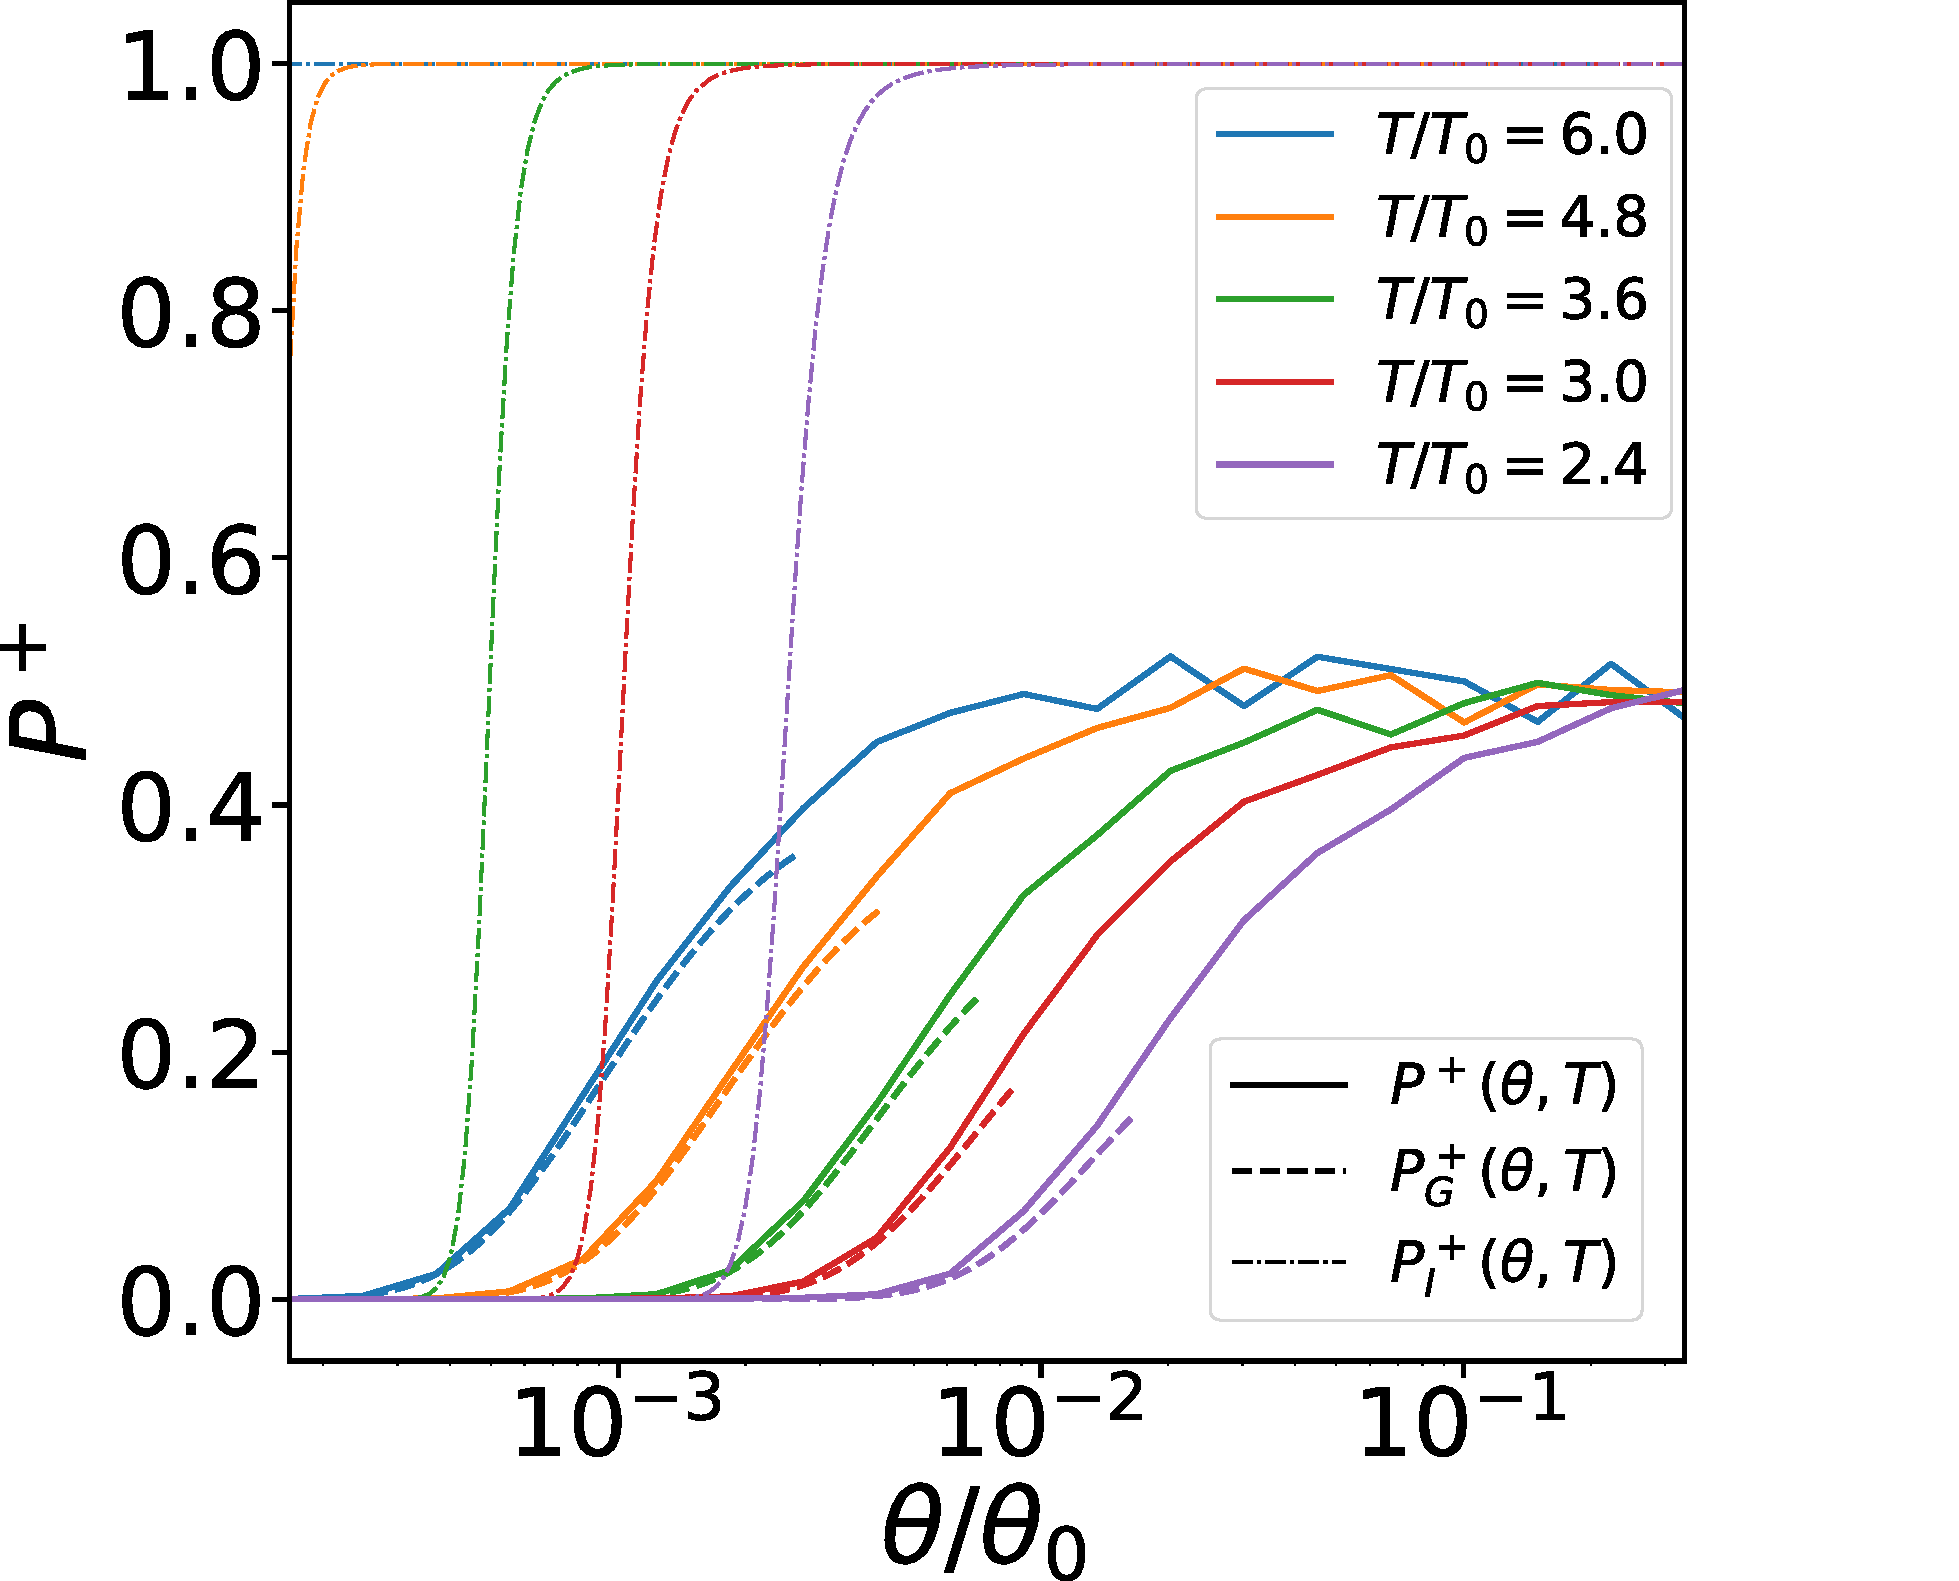
\includegraphics[width=\textwidth]{figs_part1/mcmc/switch_channel_rates_line_plot}
        \caption[]%
        {}    
    \end{subfigure}    
    
    \caption[  ]
    {\small Diffusivity-dependence of the transition path ensemble for the conservative
switch system. Panel (a) shows 50 stochastic trajectories sampled using
the TMC method for overdamped dynamics in the potential
$U(x)$ (see Appendix \ref{app:The switch system}). The dashed blue (green) lines are upper
(lower) instantons between initial (circle, $\mathbf{x}_{0}$) and
final (filled circle, $\mathbf{x}_{T}$) points. Upper and lower channels
are equally populated at temperature $\theta/\theta_{0}=0.047$ (green)
but the lower channel is preferred at the lower temperature $\theta/\theta_{0}=0.004$
(red). Trajectories of duration $T/T_{0}=3$ are sampled with $N=200(T/T_{0})$
modes. Panel (b) is a pseudocolor plot quantifying the variation of
the upper and lower channel probabilites with temperature and duration,
as obtained from TMC. The plus signs show regions where the Gaussian
mixture approximation $P_{G}^{+}$, defined in Eq. (5), is within
a $5\%$ margin of error of the simulated value. The red and green
dots correspond to the same color-coded simulations in panel (a).
Panel (c) shows a comparision between the TMC, Gaussian mixture and
instanton approximations to the upper channel probability as function
of temperature for fixed durations of path.} 
    \label{fig:switch}
\end{figure*} 
\end{comment}

We now consider the transition behavior of the 2D
system depicted in Fig.~\ref{fig:switch trajectories}. For a range of temperatures
$\theta$ and total transition times $T$ we first generate ensembles
of $10^{8}$ sample transition paths per tuple $(\theta,T)$ using
the TMC. Let $\tau_{D}(\theta)=L^{2}/(\mu k_{B}\theta)$, which is
the diffusive time-scale at temperature $\theta$. We also introduce
fixed reference temperature and time-scales $\theta_{0}=U_{0}/k_{B}$
and $T_{0}=\tau_{D}(\theta_{0})$, where $U_{0}$ is the energetic
well-depth of the potential. Our parameter range is such that $T\ll\tau_{D}$,
for each temperature $\theta$ in the range considered. Each sampled
ensemble thus describes a rare transition event. Let $\rho^{+}(\theta,T)$ and  $\rho^{-}(\theta,T)$ be the upper and lower transition channel probabilities respectively, satisfying  $\rho^{+}(\theta,T)= 1 - \rho^{+}(\theta,T)$. Furthermore, let $\mathbf{x}^+(t;\theta, T)$ and $\mathbf{x}^+(t;\theta, T)$ be the upper and lower local Onsager-Machlup instantons respectively at temperature $\theta$ and duration $T$, from which we also compute the approximate channel probability $\rho_G^{+}(\theta,T)$.

For a total transition time $T/T_{0}=3$, and for each of the two temperatures $\theta/\theta_{0}=0.047$
and $\theta/\theta_{0}=0.004$, we show 50 randomly chosen TMC sample
paths in Fig.~\ref{fig:switch trajectories}. We observe that while for the
higher temperature the paths are evenly distributed between the two
channels, for the lower temperature the lower channel is preferred. In Fig.~\ref{fig:switch channel rates} we show the numerical evaluation of $\rho^{+}(\theta,T)$ using the TMC as a function of both $\theta$
and $T$. Consistent with the $\theta/\theta_{0}=0.047$ data from
Fig.~\ref{fig:switch trajectories}, we observe that for large enough temperature
$\rho^{+}(\theta,T)\approx1/2$ (white region), so that upper and lower
channel are equally probable. That at large temperature the asymmetry
in $U$ becomes irrelevant for the TPE is expected, as in this limit
the random force in Eq.~\ref{eq:ito equation again} dominates over the
deterministic force. As $\theta$ is decreased, the channel around
$\Gamma^{-}$ becomes dominant, so that $\rho^{+}(\theta,T) \rightarrow 0$
(blue region in Fig.~\ref{fig:switch channel rates}, c.f.~$\theta/\theta_{0}=0.004$
data in panel (a)). The exact temperature at which the crossover
from the diffusivity-dominated regime to the drift-dominated regime
occurs decreases with increasing $T$; this is clearly seen in Fig.~\ref{fig:switch line plots} where vertical sections of panel (b) are shown for several values
of $T$.

We now compare our numerical TMC results for $\rho^{+}(\theta,T)$ with
the Gaussian mixture approximation $\rho_{G}^{+}$. Figure \ref{fig:switch trajectories} shows that this approximation is valid in the low-temperature regime
(plus signs). This is consistent with the assumptions underlying the
Gaussian approximation, as we expect the probability distribution
in path space to be dominated by the neighborhoods of the local instantons
only for sufficiently low temperature. As Fig.~\ref{fig:switch line plots} shows, $\rho_{G}^{+}(\theta,T)$ quantitatively captures the beginning
of the crossover from drift-dominated to diffusivity-dominated transition
behaviour for all values of $T$ considered.

For capturing this $\theta$-dependent crossover, the prefactors $\mathcal{Z}^{+}=\mathcal{Z}^{[1]}$,
$\mathcal{Z}^{-}=\mathcal{Z}^{[2]}$ in Eq.~\ref{eq:approx transition channel prob}
are essential. This becomes apparent by considering $\rho_{I}^{+}(\theta,T)$,
which only depends on the relative probabilities of the two local
instantons. In Fig.~\ref{fig:switch line plots} we see that for high enough
temperatures $\rho_{I}^{+}(\theta,T)\approx1$, meaning $S_{\text{OM}}[\mathbf{x}^{+}(t; \theta, T)]<S_{\text{OM}}[\mathbf{x}^{-}(t; \theta, T)]$
\citep{adibStochasticActionsDiffusive2008a}. This limit is understood
by comparing the two terms in the action Eq.~\ref{eq:onsager-machlup action}.
While the first term scales as $1/\theta$, the second term is independent
of $\theta$; for fixed $T$ and large enough $\theta$ the second
term thus dominates the action. This second term is smaller for the
channel around $\Gamma^{+}$ than for the channel around $\Gamma^{-}$,
because the former channel is narrower leading to to a smaller value
of $\nabla\cdot\mathbf{F}$. As $\theta$ is decreased for fixed $T$
the first term in Eq.~\ref{eq:onsager-machlup action} becomes
dominant. Figure \ref{fig:switch line plots} shows that this leads to a
crossover to $\rho_{I}^{+}(\theta,T)\approx0$, meaning $\mathbf{x}^{-}(t;\theta,T)$
becomes more probable than $\mathbf{x}^{+}(t;\theta,T)$. While this low-temperature
limit is consistent with the numerical results, the temperature at
which we observe the crossover in $\rho_{I}^{+}(\theta,T)$ is smaller
as compared to $\rho^{+}(\theta,T)$. For example, we see in Fig.~\ref{fig:switch line plots} that for $T/T_{0}=2.4$ the crossover of $\rho_{I}^{+}(\theta,T)$
is at $\theta/\theta_{0}<10^{-2}$, whereas the crossover for $\rho^{+}(\theta,T)$
occurs at $\theta/\theta_{0}>10^{-2}$. In particular this implies
that for $\theta/\theta_{0}=10^{-2}$ the most probable path goes
along $\Gamma^{+}$, while most transition paths go along $\Gamma^{-}$.
This highlights that even at intermediate-to-low temperatures, where
the Gaussian mixture approximation $\rho_G^+(\theta, T)$ is
already valid, the probabilities of the local instantons alone are
insufficient to obtain the actual transition behaviour. Instead it
is the prefactors $\mathcal{Z^{\pm}}$ in Eq.~\ref{eq:approx transition channel prob}
that dominate the crossover behaviour in Fig.~\ref{fig:switch channel rates};
these Gaussian normalisation constants are, in a sense, an entropic
contribution, as they measure the effective volume in path space of
the support around the respective local instanton. Even though for
$T/T_{0}=2.4$, $\theta/\theta_{0}=10^{-2}$ the instanton $\mathbf{x}^{+}(t;\theta,T)$
is more probable than $\mathbf{x}^{-}(t;\theta,T)$, this is more than offset
by the larger number of paths that behave similar to $\mathbf{x}^{-}(t;\theta,T)$.

\begin{comment}
\begin{figure}[t]
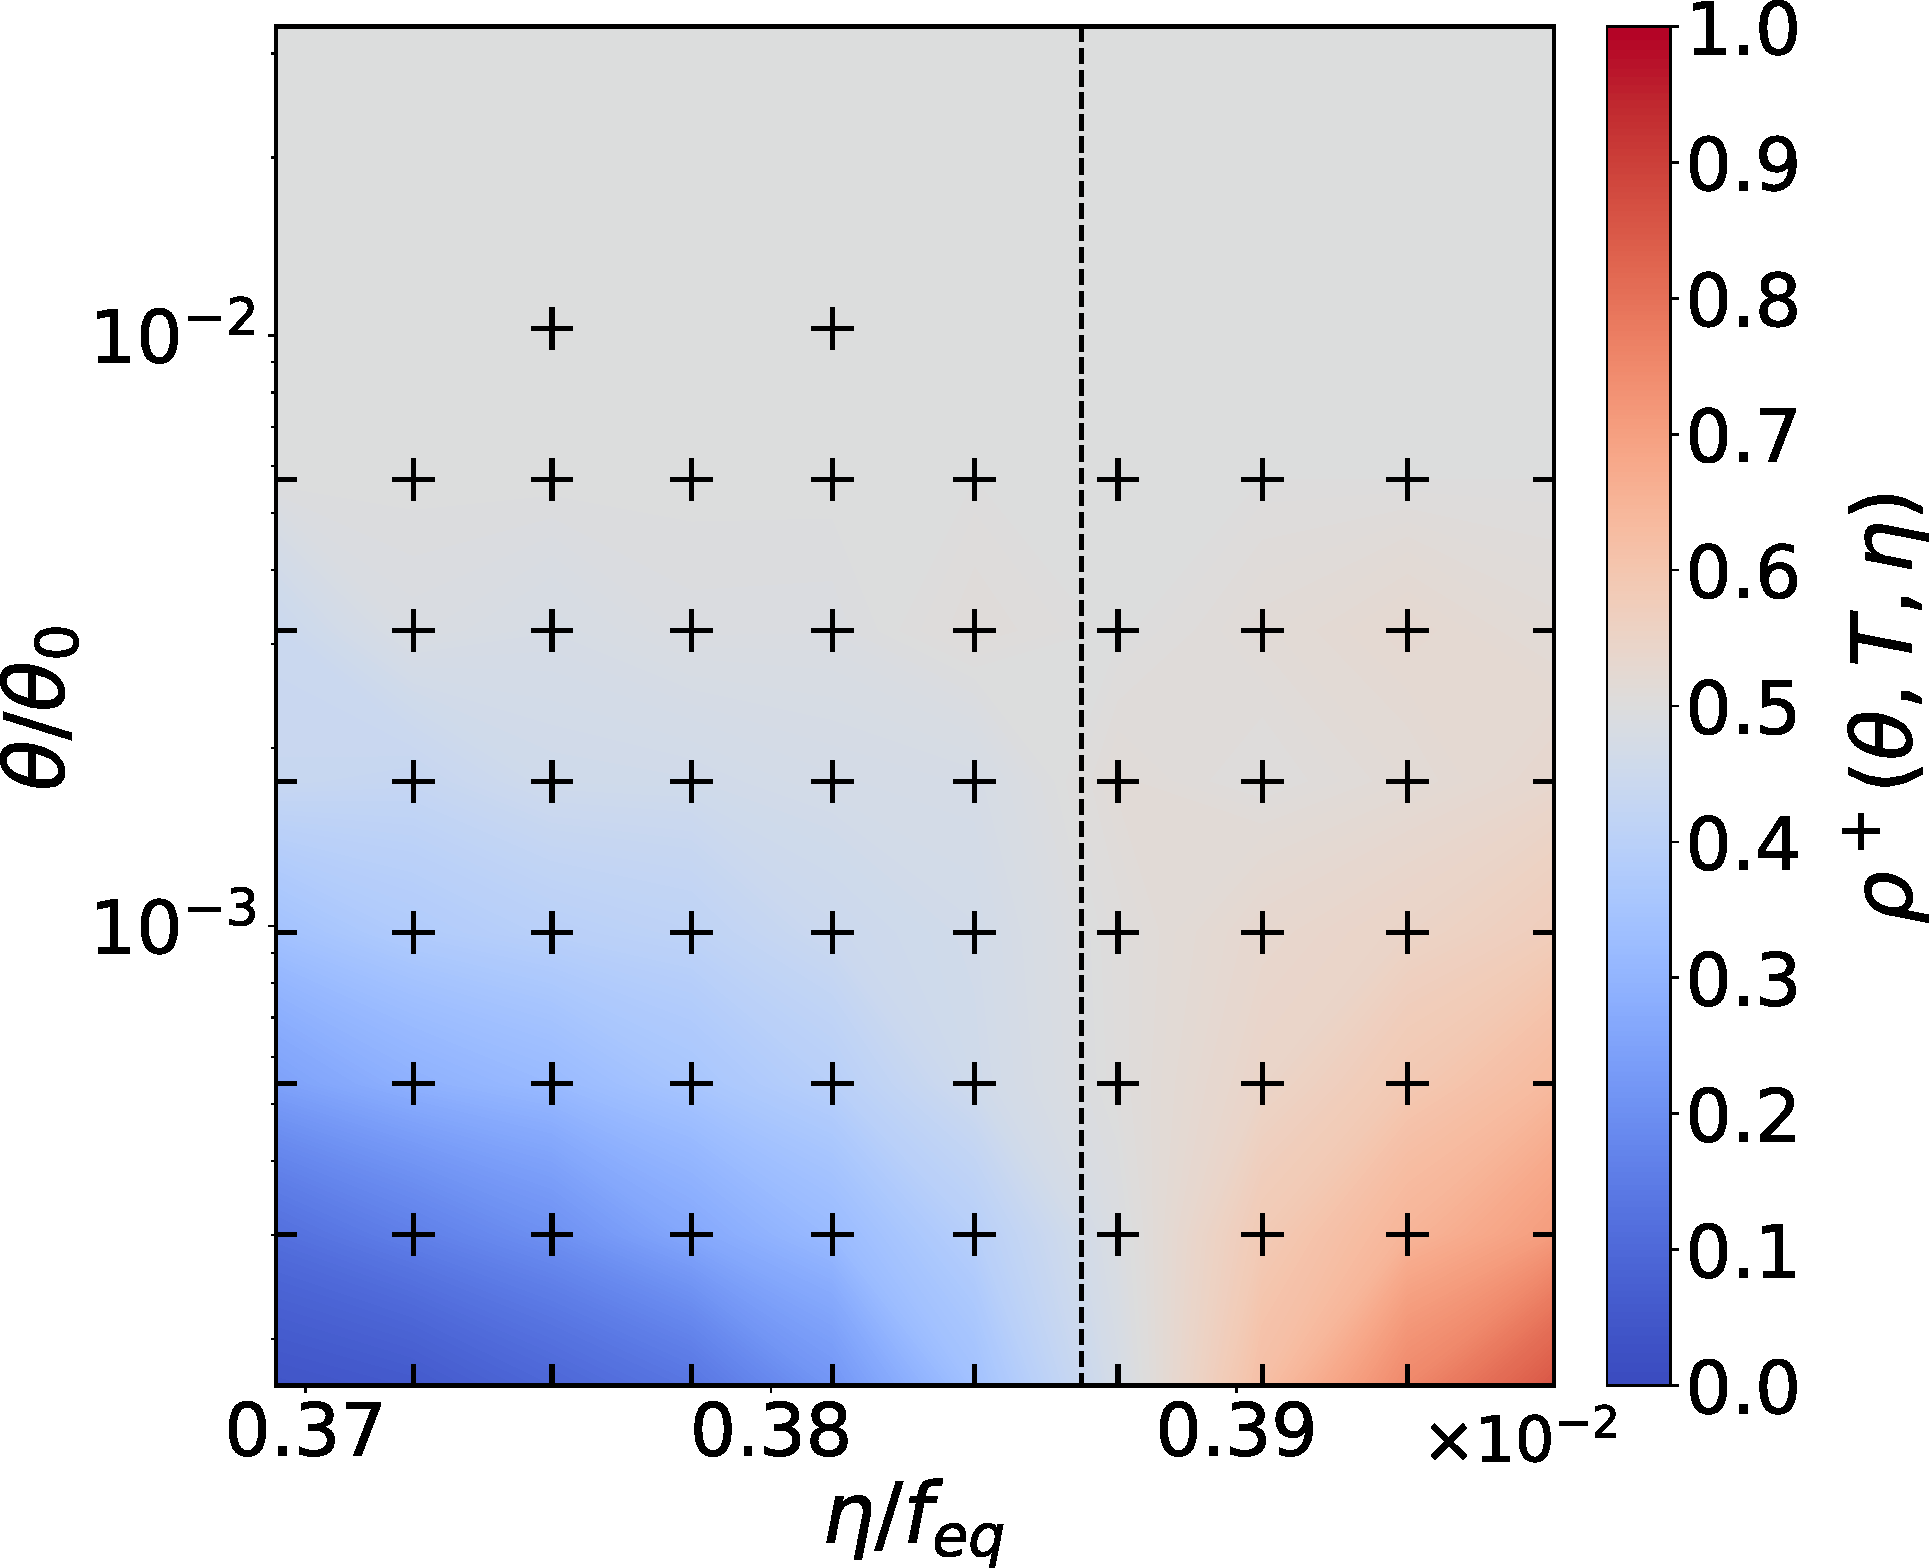
\includegraphics[width=0.36\textwidth]{figs_part1/mcmc/switch_noneq_channel_rates}
\centering \caption{Diffusivity-dependence of the transition path ensemble for the non-conservative
model system. Pseudocolour plot of the probability of the upper channel,
$P^{+}(\theta,T,\eta)$, for the non-gradient system with $T/T_{0}=3$,
as a function of the temperature $\theta$ and the circular force-strength
$\eta$. The black plus signs show regions where the variational approximation
$P_{G}^{+}(\theta,T,\eta)$, defined in Eq. \ref{eq:r function},
is within a 5\% margin of error of the simulated value. The dashed
line shows the crossover force strength $\eta_{c}/f_{\text{eq}}\approx0.00387$,
where $f_{\text{eq}}$ is the characteristic strength of the gradient
force \citep{note:SI}.}
\label{fig:switch noneq}
\end{figure}
\end{comment}

\begin{figure*} 
    \centering
     
    \begin{subfigure}[b]{0.49\textwidth}  
        \centering 
        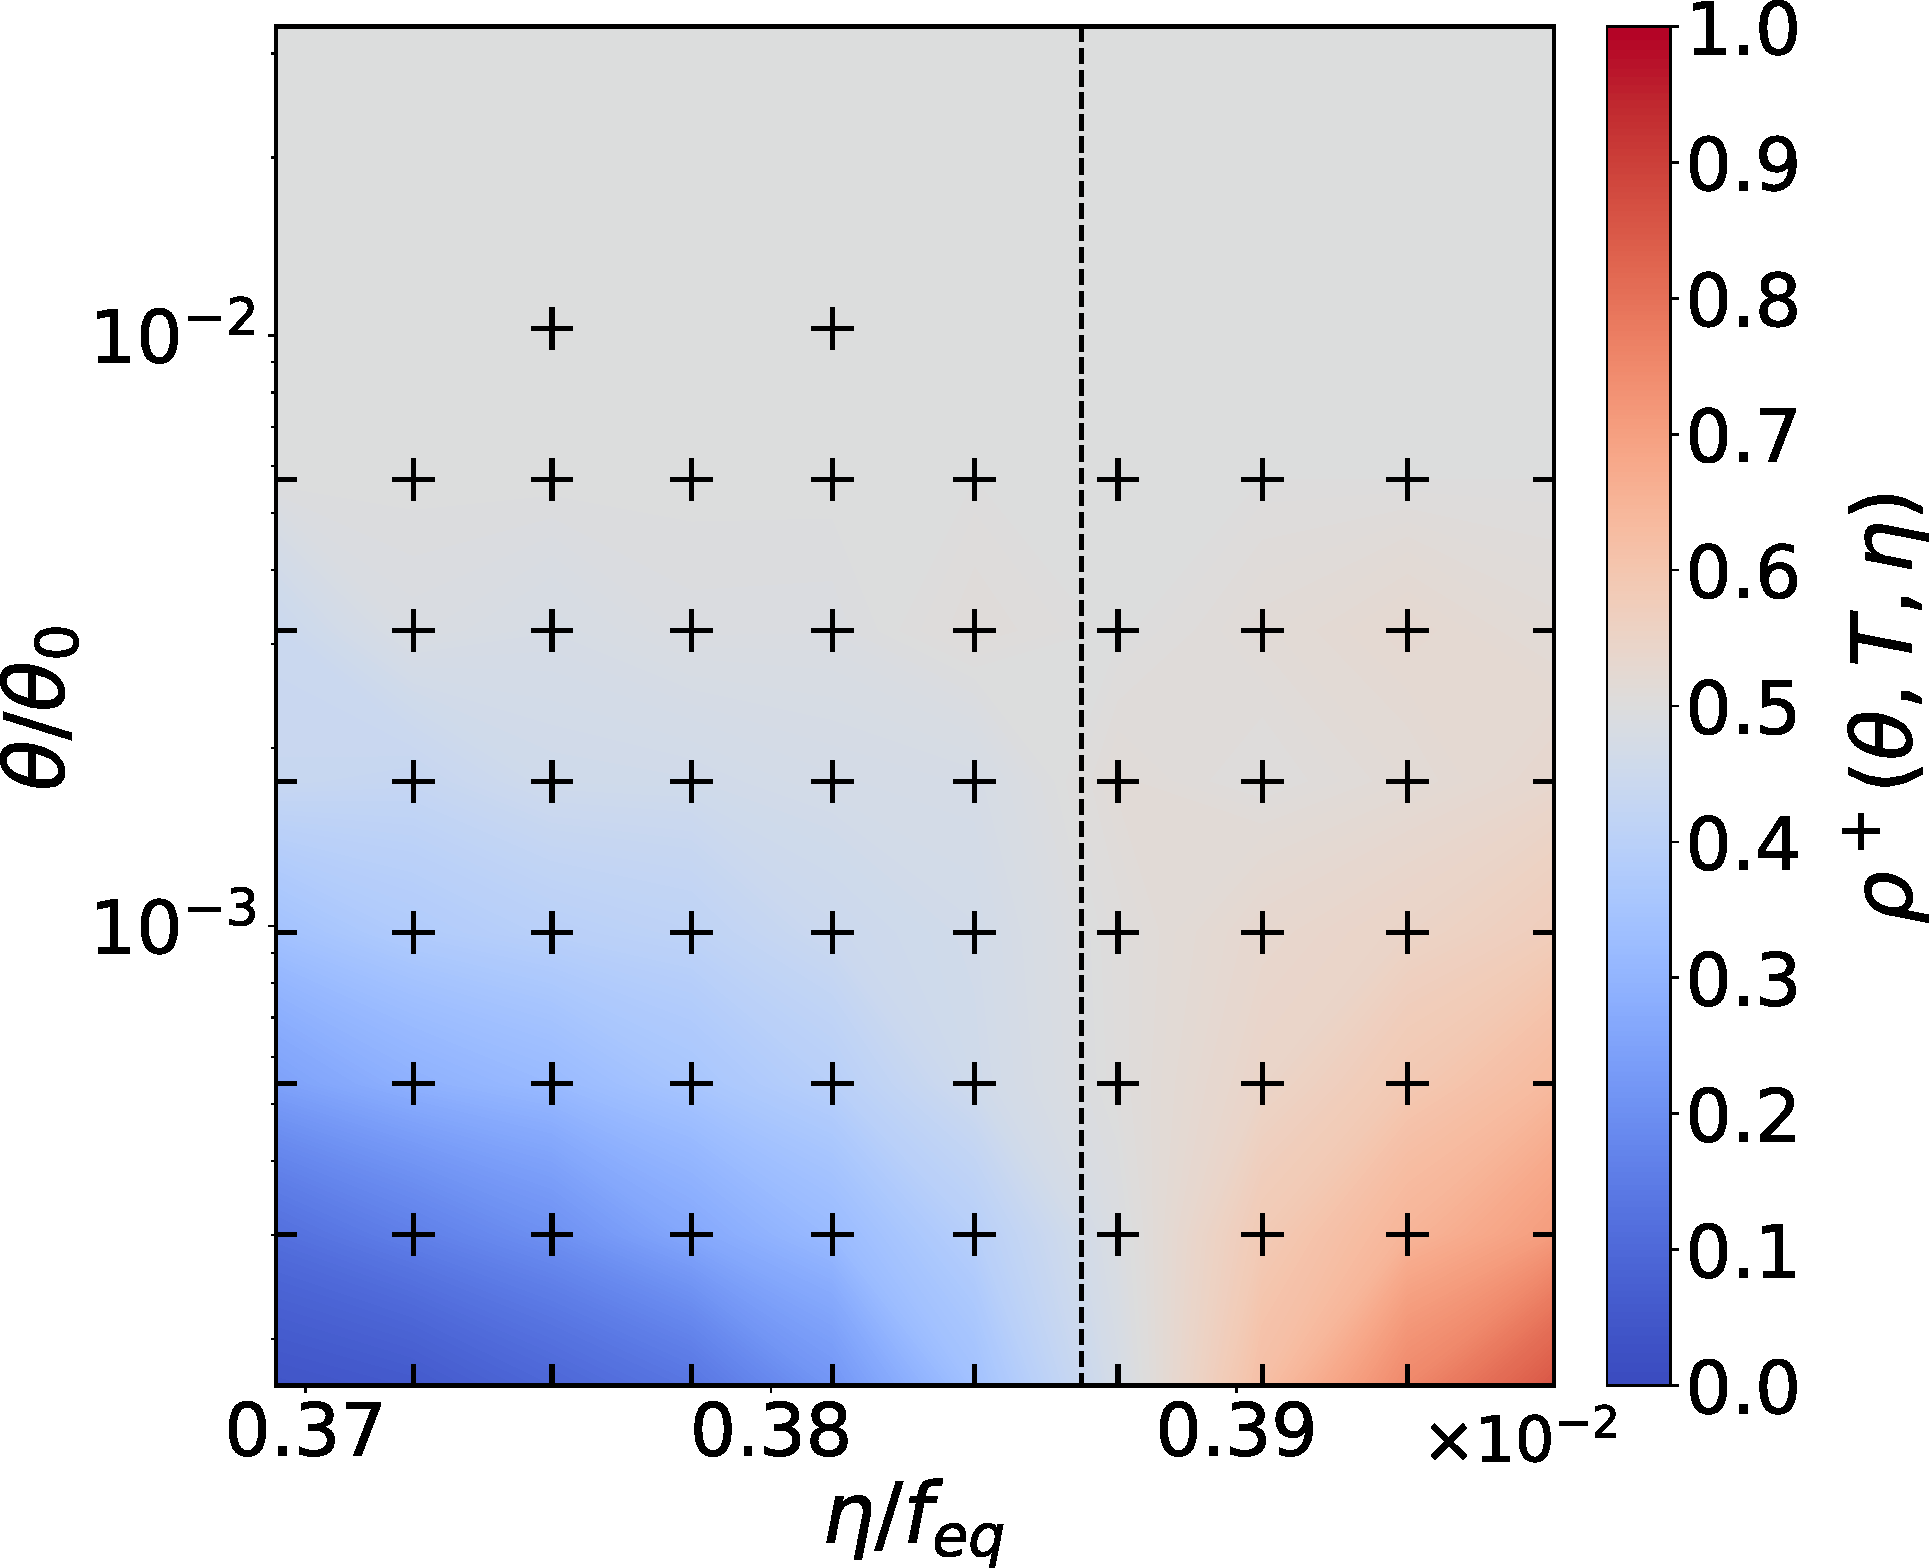
\includegraphics[width=\textwidth]{figs_part1/mcmc/switch_noneq_channel_rates}
        \caption[]%
        {}    
        \label{fig:noneq switch channel rates}
    \end{subfigure}
    \hfill
    \begin{subfigure}[b]{0.495\textwidth}
        \centering
        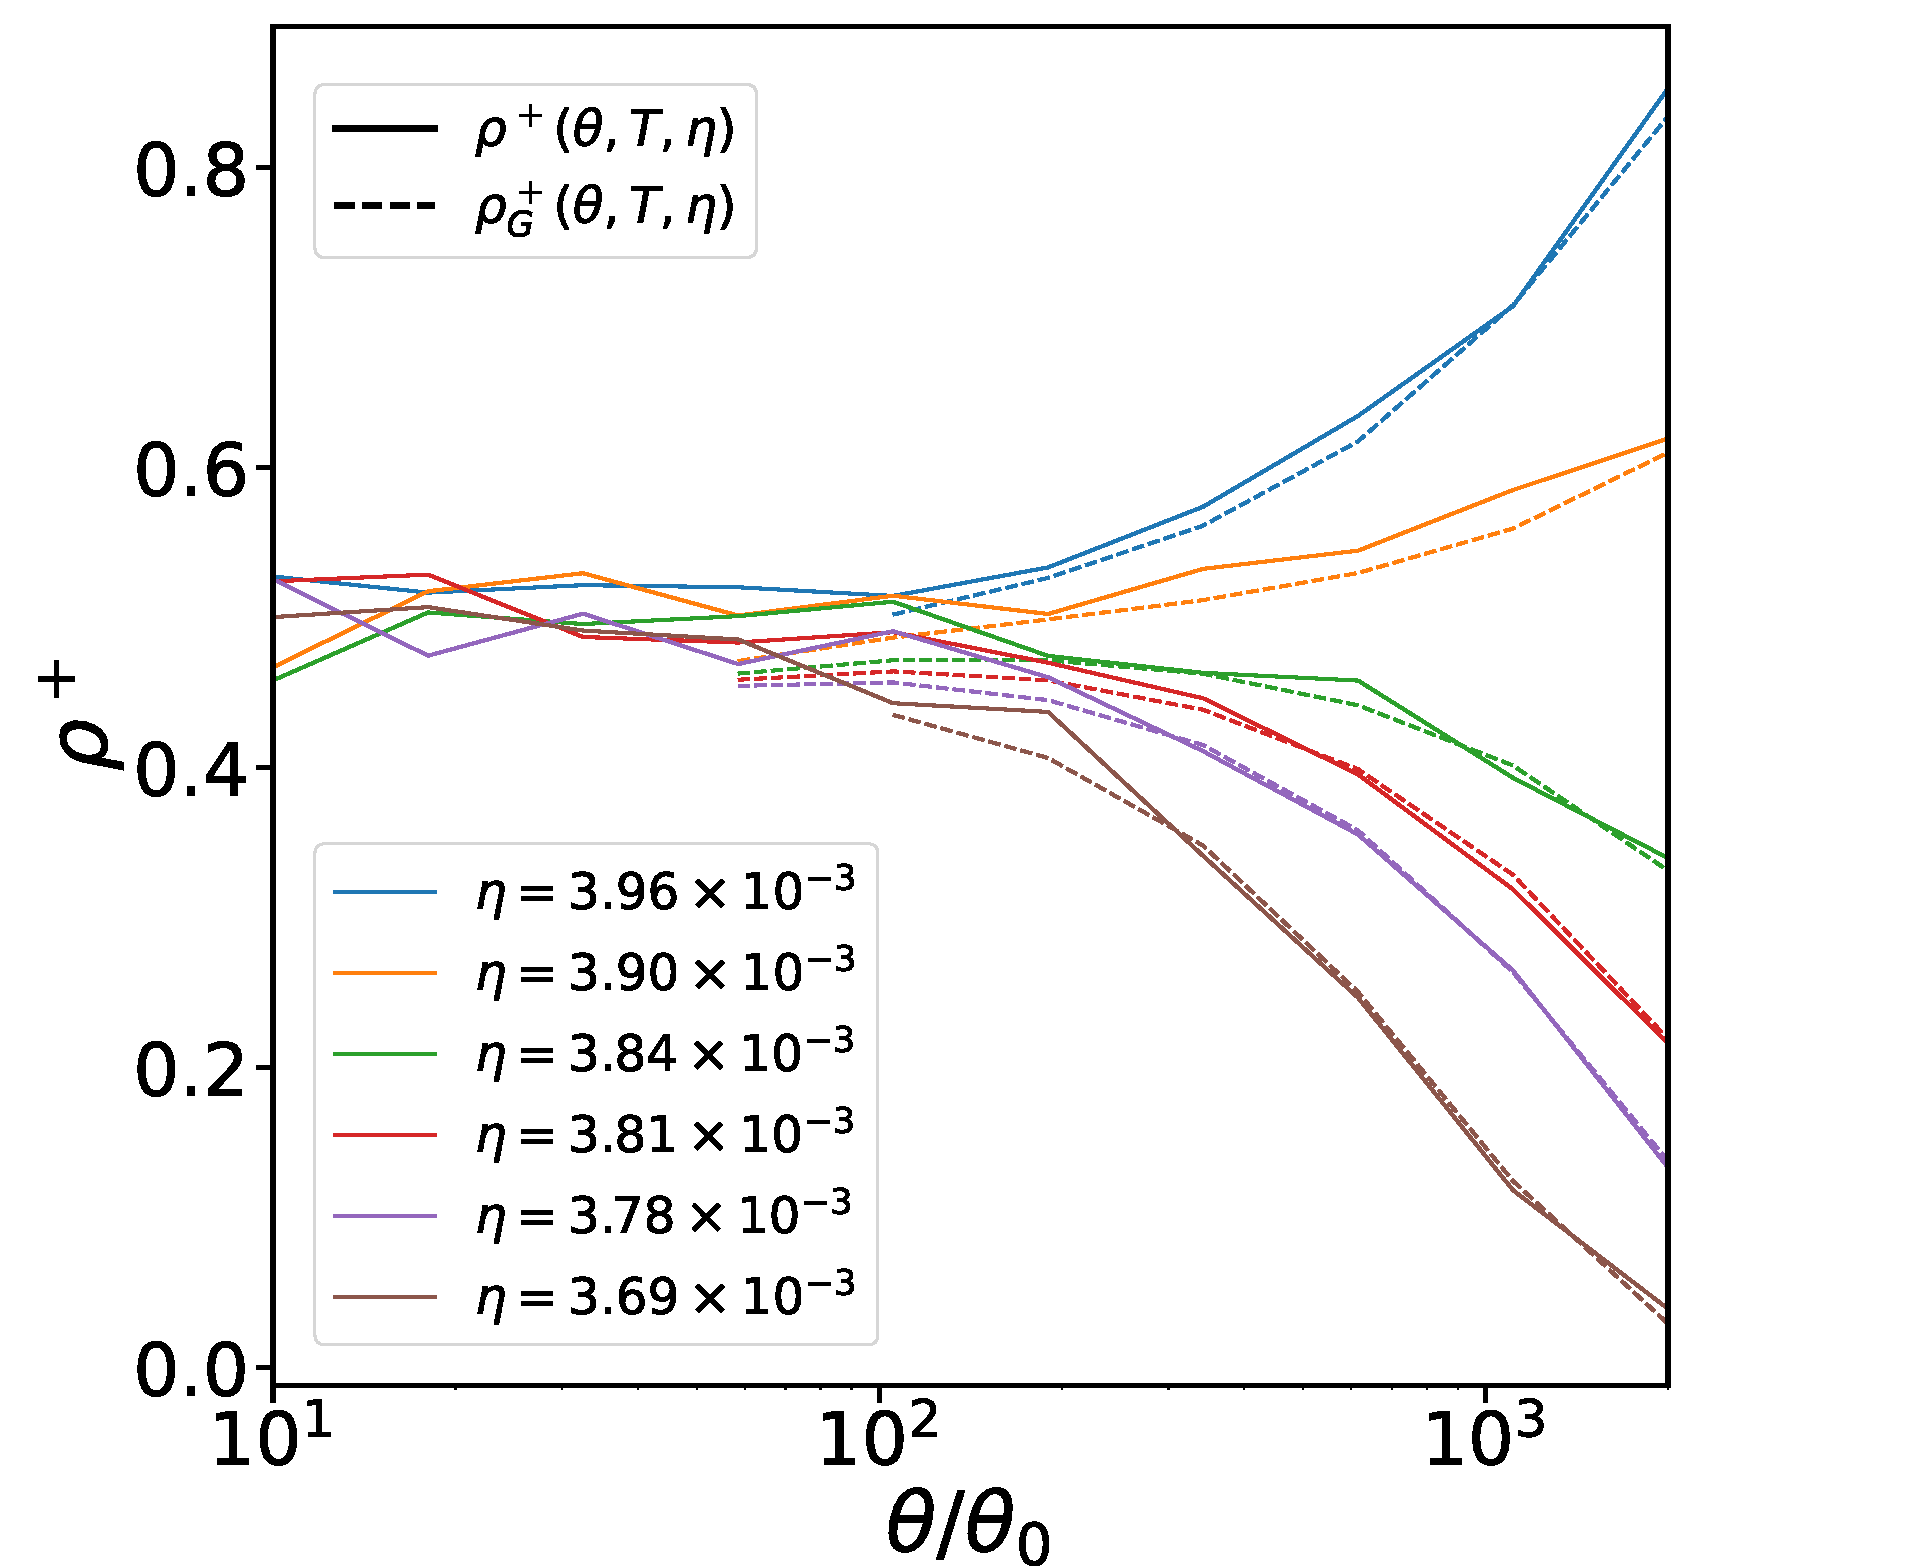
\includegraphics[width=\textwidth]{figs_part1/mcmc/switch_noneq_channel_rates_line_plot}
        \caption[]%
        {}    
        \label{fig:noneq switch line plots}
    \end{subfigure}     

    \caption[  ]
    {\small Diffusivity-dependence of the transition path ensemble for the non-conservative
model system. Panel (a) is a pseudocolour plot of the probability of the upper channel
$\rho^{+}(\theta,T,\eta)$, computed using the TMC, for the non-gradient system with $T/T_{0}=3$,
as a function of the temperature $\theta$ and the circular force-strength
$\eta$. The black plus signs show regions where the variational approximation
$\rho_{G}^{+}(\theta,T,\eta)$, defined in Eq.~\ref{eq:approx transition channel prob},
is within a 5\% margin of error of the simulated value. The dashed
line shows the crossover force strength $\eta_{c}/f_{\text{eq}}\approx0.00387$,
where $f_{\text{eq}}$ is the characteristic strength of the gradient
force. Panel (b) Compares the upper channel probability $\rho^{[\alpha]}(\theta,T)$ with the Gaussian mixture and
instanton approximations to the upper channel probability as function
of temperature for $T/T_{0}=3$ and a range of values for $\eta_c$.} \label{eq:switch noneq}
\end{figure*} 



\begin{comment}
As we discuss in the \citep{note:SI}, in the Freidlin-Wentzell-Graham
limit \citep{wentzellSmallRandomPerturbations1970,grahamMacroscopicPotentialsBifurcations1989}
of vanishing temperature and infinite path duration both instantons
become equally probable, $\lim_{T\to\infty}\lim_{\theta\to0}r_{S}(\theta,T)=1/2$.
Nonetheless, also in this limit we expect the TPE to still be entirely
concentrated around $\Gamma^{<}$ because of the unequal normalisation
constants $\mathcal{Z}$ along the two channels \citep{note:SI}.
\end{comment}

For the non-gradient forms of the drift, the prefactors $\mathcal{Z^{\pm}}$
can also drive the crossover behaviour of the system, as we show now
by adding a force of strength $\eta$ that acts perpendicular to the
radius vector in the clockwise direction. For positive force strength
$\eta$, this non-conservative force biases towards the upper channel
$\Gamma^{+}$. In Fig.~\ref{fig:noneq switch channel rates} we show numerical
results for $\rho^{+}(\theta,T,\eta)$ as a function of $\eta$ and $\theta$
for $T/T_{0}=3$. For small $\eta/f_{\text{eq}}\rightarrow0$, where
$f_{\text{eq}}$ is the characteristic strength of the gradient force
(see Appendix \ref{app:The switch system} for more details), we recover the results from Fig.~\ref{fig:switch channel rates} and Fig.~\ref{fig:switch line plots}. Thus at small but finite temperature the dominant transition
channel is the one where particles travel againt the weak non-conservative
force. As $\eta$ is increased to $\eta_{c}/f_{\text{eq}}\approx0.00387$,
we observe a crossover from $\Gamma^{-}$-channel dominated transitions
to $\Gamma^{+}$-channel dominated transitions in the low-temperature
regime. This switch is also captured by the Gaussian approximation
(plus signs in Fig.~\ref{fig:noneq switch channel rates}). On the other hand,
throughout the parameter regime considered in Fig.~\ref{fig:noneq switch channel rates},
we find that $\rho_{I}^{+}(\theta,T,\eta)\approx1$, meaning that the
local instanton $\mathbf{x}^{+}(t;\theta,T)$ is always more probable than $\mathbf{x}^{-}(t;\theta,T)$ for finite $\eta$. This again highlights the relevance of considering Gaussian fluctuations around the instantons for determining the dominant
transition pathway.

\section{Conclusion}

For a system with two competing transition pathways,
we have studied how the dominant transition pathway depends on both
the temperature and the total duration. To quantify the relative importance
of the competing pathways, we have constructed semi-analytical approximators
which are valid in the low-to-intermediate temperature regime. We
have validated our approximators via comparison with a continuous-time
MCMC method that is dimensionally robust and efficiently samples systems
with multiple reactive pathways.

Our results show that even in the low-to-intermediate temperature
regime the global instanton, or most probable path, itself is not
sufficient to determine the dominant transition pathway. Rather, it
is vital that fluctuations around this path be incorporated. This
has a simple one-dimensional equivalent: For a probability density
$p(x)\sim\exp(-V(x))$ for some potential $V(x)$ with relative
minima $x_{\alpha}$, the probabilistically most relevant minimum
is not the global one, but that with the largest well probability,
i.e.$~$the $x_{\alpha}$ that maximizes $P(\,\mathrm{well~around~}x_{\alpha}\,)\sim e^{-V(x_{\alpha})}\sqrt{{2\pi}/{V''(x_{\alpha})}}$,
where we use a quadratic Taylor approximation of $V$ around $x_{\alpha}$.
The most probable well is thus determined by an interplay of $e^{-V(x_{\alpha})}$
(which corresponds to the instanton probability $e^{-S_{\text{OM}}[\mathbf{x}^{[\alpha]}]}$)
and $\sqrt{{2\pi}/{V''(x_{\alpha})}}$ (which corresponds to the regularised
normalisation constant $\mathcal{Z}^{[\alpha]}$).

In this chapter we considered a paradigmatic example system with
two competing transition pathways. The method of instantons is an
established technique in theoretical chemistry and statistical physics
\citep{eMinimumActionMethod2004a, weinanStringMethodStudy2002, grafke_instanton_2015, grafke_numerical_2019, schorlepp_gelfandyaglom_2021, dematteis_experimental_2019, ferreApproximateOptimalControls2021a, kikuchiRitzMethodTransition2020a, heymannGeometricMinimumAction2008a},
and the method of Gaussian mixtures presented here scales as $O(d^{2})$
with the number of degrees of freedom $d$. It is
therefore feasible to apply the methods we developed here to more
realistic many-particle systems to study e.g.~nucleation pathways
\citep{weinanStringMethodStudy2002, lutskoHowCrystalsForm2019a, rein_ten_wolde_numerical_1996}
or conformational rearrangements in macromolecules \citep{ren_transition_2005, fujisakiOnsagerMachlupActionbased2010a, fujisakiMultiscaleEnhancedPath2013a, gartnerModelingSimulationsPolymers2019}.

Our quantification here of the finite-temperature breakdown of instanton
theories is important for relating such theories to experiments, which
are always at finite temperatures. Our insights into path-space probability
distributions for diffusive stochastic dynamics, together with our
MCMC method, will therefore be valuable for going beyond the regime
of asymptotically low diffusivity in both large deviations theory
\citep{wentzellSmallRandomPerturbations1970, heymannGeometricMinimumAction2008a, gartnerModelingSimulationsPolymers2019}
and the study of rare events \citep{grafkeSharpAsymptoticEstimates2021}.









